\documentclass[a4paper]{book}
\usepackage{a4wide}
\usepackage{makeidx}
\usepackage{graphicx}
\usepackage{multicol}
\usepackage{float}
\usepackage{listings}
\usepackage{color}
\usepackage{textcomp}
\usepackage{alltt}
\usepackage{times}
\usepackage{ifpdf}
\ifpdf
\usepackage[pdftex,
            pagebackref=true,
            colorlinks=true,
            linkcolor=blue,
            unicode
           ]{hyperref}
\else
\usepackage[ps2pdf,
            pagebackref=true,
            colorlinks=true,
            linkcolor=blue,
            unicode
           ]{hyperref}
\usepackage{pspicture}
\fi
\usepackage[utf8]{inputenc}
\usepackage{doxygen}
\lstset{language=C++,inputencoding=utf8,basicstyle=\footnotesize,breaklines=true,breakatwhitespace=true,tabsize=8,numbers=left }
\makeindex
\setcounter{tocdepth}{3}
\renewcommand{\footrulewidth}{0.4pt}
\begin{document}
\hypersetup{pageanchor=false}
\begin{titlepage}
\vspace*{7cm}
\begin{center}
{\Large ZorkTrek \\[1ex]\large 1.0 }\\
\vspace*{1cm}
{\large Generated by Doxygen 1.6.3}\\
\vspace*{0.5cm}
{\small Sat Aug 7 20:03:29 2010}\\
\end{center}
\end{titlepage}
\clearemptydoublepage
\pagenumbering{roman}
\tableofcontents
\clearemptydoublepage
\pagenumbering{arabic}
\hypersetup{pageanchor=true}
\chapter{Class Index}
\section{Class Hierarchy}
This inheritance list is sorted roughly, but not completely, alphabetically:\begin{DoxyCompactList}
\item \contentsline{section}{Battle}{\pageref{dd/dfd/classBattle}}{}
\item \contentsline{section}{BitMaze}{\pageref{d2/ddb/classBitMaze}}{}
\item \contentsline{section}{CelestialBody}{\pageref{d4/d0b/classCelestialBody}}{}
\begin{DoxyCompactList}
\item \contentsline{section}{Moon}{\pageref{d8/d6f/classMoon}}{}
\item \contentsline{section}{Planet}{\pageref{d5/dec/classPlanet}}{}
\end{DoxyCompactList}
\item \contentsline{section}{cell\_\-t}{\pageref{d9/d8a/structcell__t}}{}
\item \contentsline{section}{Command}{\pageref{d9/d71/classCommand}}{}
\item \contentsline{section}{CommandWords}{\pageref{d0/dda/classCommandWords}}{}
\item \contentsline{section}{Parser}{\pageref{d0/d40/classParser}}{}
\item \contentsline{section}{PVEEntity}{\pageref{df/dde/classPVEEntity}}{}
\begin{DoxyCompactList}
\item \contentsline{section}{BorgCube}{\pageref{d2/d93/classBorgCube}}{}
\item \contentsline{section}{BorgProbe}{\pageref{db/deb/classBorgProbe}}{}
\item \contentsline{section}{BorgQueen}{\pageref{d6/d8d/classBorgQueen}}{}
\item \contentsline{section}{BorgRogue}{\pageref{db/d4f/classBorgRogue}}{}
\item \contentsline{section}{BorgScout}{\pageref{d5/d8c/classBorgScout}}{}
\item \contentsline{section}{BorgSphere}{\pageref{d6/ddd/classBorgSphere}}{}
\item \contentsline{section}{BorgTactical}{\pageref{d0/d4e/classBorgTactical}}{}
\end{DoxyCompactList}
\item \contentsline{section}{SdlGLMap}{\pageref{d9/d4a/classSdlGLMap}}{}
\item \contentsline{section}{SolarSystem}{\pageref{df/d5e/classSolarSystem}}{}
\item \contentsline{section}{StarShip}{\pageref{da/d97/classStarShip}}{}
\item \contentsline{section}{StarTrekEntities}{\pageref{d0/ddd/classStarTrekEntities}}{}
\item \contentsline{section}{ZorkTrek}{\pageref{d6/df9/classZorkTrek}}{}
\end{DoxyCompactList}

\chapter{Class Index}
\section{Class List}
Here are the classes, structs, unions and interfaces with brief descriptions:\begin{DoxyCompactList}
\item\contentsline{section}{\hyperlink{classBattle}{Battle} }{\pageref{dd/dfd/classBattle}}{}
\item\contentsline{section}{\hyperlink{classBitMaze}{BitMaze} }{\pageref{d2/ddb/classBitMaze}}{}
\item\contentsline{section}{\hyperlink{classBorgCube}{BorgCube} }{\pageref{d2/d93/classBorgCube}}{}
\item\contentsline{section}{\hyperlink{classBorgProbe}{BorgProbe} }{\pageref{db/deb/classBorgProbe}}{}
\item\contentsline{section}{\hyperlink{classBorgQueen}{BorgQueen} }{\pageref{d6/d8d/classBorgQueen}}{}
\item\contentsline{section}{\hyperlink{classBorgRogue}{BorgRogue} }{\pageref{db/d4f/classBorgRogue}}{}
\item\contentsline{section}{\hyperlink{classBorgScout}{BorgScout} }{\pageref{d5/d8c/classBorgScout}}{}
\item\contentsline{section}{\hyperlink{classBorgSphere}{BorgSphere} }{\pageref{d6/ddd/classBorgSphere}}{}
\item\contentsline{section}{\hyperlink{classBorgTactical}{BorgTactical} }{\pageref{d0/d4e/classBorgTactical}}{}
\item\contentsline{section}{\hyperlink{classCelestialBody}{CelestialBody} }{\pageref{d4/d0b/classCelestialBody}}{}
\item\contentsline{section}{\hyperlink{structcell__t}{cell\_\-t} }{\pageref{d9/d8a/structcell__t}}{}
\item\contentsline{section}{\hyperlink{classCommand}{Command} }{\pageref{d9/d71/classCommand}}{}
\item\contentsline{section}{\hyperlink{classCommandWords}{CommandWords} }{\pageref{d0/dda/classCommandWords}}{}
\item\contentsline{section}{\hyperlink{classMoon}{Moon} }{\pageref{d8/d6f/classMoon}}{}
\item\contentsline{section}{\hyperlink{classParser}{Parser} }{\pageref{d0/d40/classParser}}{}
\item\contentsline{section}{\hyperlink{classPlanet}{Planet} }{\pageref{d5/dec/classPlanet}}{}
\item\contentsline{section}{\hyperlink{classPVEEntity}{PVEEntity} }{\pageref{df/dde/classPVEEntity}}{}
\item\contentsline{section}{\hyperlink{classSdlGLMap}{SdlGLMap} }{\pageref{d9/d4a/classSdlGLMap}}{}
\item\contentsline{section}{\hyperlink{classSolarSystem}{SolarSystem} }{\pageref{df/d5e/classSolarSystem}}{}
\item\contentsline{section}{\hyperlink{classStarShip}{StarShip} }{\pageref{da/d97/classStarShip}}{}
\item\contentsline{section}{\hyperlink{classStarTrekEntities}{StarTrekEntities} }{\pageref{d0/ddd/classStarTrekEntities}}{}
\item\contentsline{section}{\hyperlink{classZorkTrek}{ZorkTrek} }{\pageref{d6/df9/classZorkTrek}}{}
\end{DoxyCompactList}

\chapter{Class Documentation}
\hypertarget{classBattle}{
\section{Battle Class Reference}
\label{dd/dfd/classBattle}\index{Battle@{Battle}}
}


{\ttfamily \#include $<$Battle.h$>$}

\subsection*{Public Member Functions}
\begin{DoxyCompactItemize}
\item 
\hyperlink{classBattle_abecc253b23b71da260445e4bdc8522e2}{Battle} ()
\item 
\hyperlink{classBattle_a46d700ea31d3be9e3c2b7f58a361490e}{Battle} (\hyperlink{classStarShip}{StarShip} $\ast$ship, \hyperlink{classPVEEntity}{PVEEntity} $\ast$enemy)
\item 
\hyperlink{classBattle_ae44141e587836ba84243cad46b17c228}{$\sim$Battle} ()
\item 
void \hyperlink{classBattle_a21c7d3fe2b8f8acdcf52d7dc03ee0845}{enemyMove} ()
\item 
void \hyperlink{classBattle_ac47c4c6769ba4c285b6b3bce196665f7}{Phaser} (bool who)
\item 
void \hyperlink{classBattle_af93833dc6f45a9a9b57b3fd0a98c7b53}{Phased} (bool who)
\item 
void \hyperlink{classBattle_abb853e7323e8c06115d261476eb60da6}{Pulse} (bool who)
\item 
void \hyperlink{classBattle_a4e3b6df23a451e85b0bd078e4a5692fa}{Photon} (bool who)
\item 
void \hyperlink{classBattle_ab146205ff35979b462ee057f3dedf84c}{Quantum} (bool who)
\item 
void \hyperlink{classBattle_a291ea216c6a4a576c9cd287ddf5afb89}{Transphasic} (bool who)
\item 
void \hyperlink{classBattle_ac27cb8ae9cc2220d90446de6d5c2a03e}{Chroniton} (bool who)
\item 
void \hyperlink{classBattle_a59fbad01d3da6683a902601dee2a244c}{Gravimetric} (bool who)
\item 
void \hyperlink{classBattle_af3866096de0e01ea273b211d0babaade}{Spatial} (bool who)
\item 
void \hyperlink{classBattle_a36916b73287143368e13759da9a64842}{Tractor} (bool who, bool tractor)
\item 
bool \hyperlink{classBattle_a4c6da8cc9af5dd34901c18a9d54ea139}{enemyHasTractor} ()
\item 
\hyperlink{classPVEEntity}{PVEEntity} $\ast$ \hyperlink{classBattle_aafeb9f025d6d77ba8a58a3fbd386c039}{getEnemy} ()
\item 
string \hyperlink{classBattle_a5d850d794776aac6b7d742f3385ce82a}{getEnemyName} ()
\end{DoxyCompactItemize}


\subsection{Detailed Description}
\hyperlink{classBattle}{Battle} handles fight interaction holds a pointer to the player holds a pointer to the current targeted enemy 

\subsection{Constructor \& Destructor Documentation}
\hypertarget{classBattle_abecc253b23b71da260445e4bdc8522e2}{
\index{Battle@{Battle}!Battle@{Battle}}
\index{Battle@{Battle}!Battle@{Battle}}
\subsubsection[{Battle}]{\setlength{\rightskip}{0pt plus 5cm}Battle::Battle ()}}
\label{dd/dfd/classBattle_abecc253b23b71da260445e4bdc8522e2}
Default Constructor \hypertarget{classBattle_a46d700ea31d3be9e3c2b7f58a361490e}{
\index{Battle@{Battle}!Battle@{Battle}}
\index{Battle@{Battle}!Battle@{Battle}}
\subsubsection[{Battle}]{\setlength{\rightskip}{0pt plus 5cm}Battle::Battle ({\bf StarShip} $\ast$ {\em ship}, \/  {\bf PVEEntity} $\ast$ {\em enemy})}}
\label{dd/dfd/classBattle_a46d700ea31d3be9e3c2b7f58a361490e}
A new instance of a battle must have a pointer to the current players SharShip and the enemy being engaged


\begin{DoxyParams}{Parameters}
\item[{\em $\ast$ship}]a pointer to the current player's \hyperlink{classStarShip}{StarShip} \item[{\em $\ast$enemy}]a pointer to the \hyperlink{classPVEEntity}{PVEEntity} currently being engaged \end{DoxyParams}
\begin{DoxyReturn}{Returns}
constructor does not have a return type 
\end{DoxyReturn}
\begin{DoxySeeAlso}{See also}
Battle::getIsWreckPVE 
\end{DoxySeeAlso}
\hypertarget{classBattle_ae44141e587836ba84243cad46b17c228}{
\index{Battle@{Battle}!$\sim$Battle@{$\sim$Battle}}
\index{$\sim$Battle@{$\sim$Battle}!Battle@{Battle}}
\subsubsection[{$\sim$Battle}]{\setlength{\rightskip}{0pt plus 5cm}Battle::$\sim$Battle ()}}
\label{dd/dfd/classBattle_ae44141e587836ba84243cad46b17c228}
\begin{DoxyReturn}{Returns}
deconstructor does not have a return type 
\end{DoxyReturn}


\subsection{Member Function Documentation}
\hypertarget{classBattle_ac27cb8ae9cc2220d90446de6d5c2a03e}{
\index{Battle@{Battle}!Chroniton@{Chroniton}}
\index{Chroniton@{Chroniton}!Battle@{Battle}}
\subsubsection[{Chroniton}]{\setlength{\rightskip}{0pt plus 5cm}void Battle::Chroniton (bool {\em who})}}
\label{dd/dfd/classBattle_ac27cb8ae9cc2220d90446de6d5c2a03e}
enemy or the player fires chroniton torps @ WHO


\begin{DoxyParams}{Parameters}
\item[{\em who}]true = player false = current enemy\end{DoxyParams}
\begin{DoxyReturn}{Returns}
void
\end{DoxyReturn}
\begin{DoxySeeAlso}{See also}
Battle::describeAction 

Battle::setShielding

PVEEntity::getIsWreckPVE 
\end{DoxySeeAlso}
\hypertarget{classBattle_a4c6da8cc9af5dd34901c18a9d54ea139}{
\index{Battle@{Battle}!enemyHasTractor@{enemyHasTractor}}
\index{enemyHasTractor@{enemyHasTractor}!Battle@{Battle}}
\subsubsection[{enemyHasTractor}]{\setlength{\rightskip}{0pt plus 5cm}bool Battle::enemyHasTractor ()}}
\label{dd/dfd/classBattle_a4c6da8cc9af5dd34901c18a9d54ea139}
finds weather the enemy has a tractor on the player

\begin{DoxyReturn}{Returns}
bool enemy has a tractor lock
\end{DoxyReturn}
\begin{DoxySeeAlso}{See also}
PVEEntity::getHasTractorLock 
\end{DoxySeeAlso}
\hypertarget{classBattle_a21c7d3fe2b8f8acdcf52d7dc03ee0845}{
\index{Battle@{Battle}!enemyMove@{enemyMove}}
\index{enemyMove@{enemyMove}!Battle@{Battle}}
\subsubsection[{enemyMove}]{\setlength{\rightskip}{0pt plus 5cm}void Battle::enemyMove ()}}
\label{dd/dfd/classBattle_a21c7d3fe2b8f8acdcf52d7dc03ee0845}
Randomly Performs a enemy move returns if the enemy is destroyed only performs an action if the enemy have that type of weapon seedMicroPrecision decides the action of the switch

\begin{DoxyReturn}{Returns}
void
\end{DoxyReturn}
\begin{DoxySeeAlso}{See also}
Battle::getIsWreckPVE

\hyperlink{classBattle_ac47c4c6769ba4c285b6b3bce196665f7}{Battle::Phaser} 

\hyperlink{classBattle_af93833dc6f45a9a9b57b3fd0a98c7b53}{Battle::Phased} 

\hyperlink{classBattle_abb853e7323e8c06115d261476eb60da6}{Battle::Pulse} 

\hyperlink{classBattle_a291ea216c6a4a576c9cd287ddf5afb89}{Battle::Transphasic} 

\hyperlink{classBattle_ac27cb8ae9cc2220d90446de6d5c2a03e}{Battle::Chroniton} 

\hyperlink{classBattle_a59fbad01d3da6683a902601dee2a244c}{Battle::Gravimetric} 

\hyperlink{classBattle_af3866096de0e01ea273b211d0babaade}{Battle::Spatial} 

\hyperlink{classBattle_a36916b73287143368e13759da9a64842}{Battle::Tractor}

seedMicroPrecision

PVEEntity::getHasLasers 

PVEEntity::getHasPhasedIonCannon 

PVEEntity::getHasPulseWeapon 

PVEEntity::getHasTransphasicTorpedos 

PVEEntity::getHasChronitonTorpedos 

PVEEntity::getHasGravimetricTorpedos 

PVEEntity::getHasSpatialTorpedos 

PVEEntity::getHasTractorLock 
\end{DoxySeeAlso}
\hypertarget{classBattle_aafeb9f025d6d77ba8a58a3fbd386c039}{
\index{Battle@{Battle}!getEnemy@{getEnemy}}
\index{getEnemy@{getEnemy}!Battle@{Battle}}
\subsubsection[{getEnemy}]{\setlength{\rightskip}{0pt plus 5cm}{\bf PVEEntity} $\ast$ Battle::getEnemy ()}}
\label{dd/dfd/classBattle_aafeb9f025d6d77ba8a58a3fbd386c039}
returns a pointer to the battles enemy

\begin{DoxyReturn}{Returns}
PVEEntity$\ast$ the enemy 
\end{DoxyReturn}
\hypertarget{classBattle_a5d850d794776aac6b7d742f3385ce82a}{
\index{Battle@{Battle}!getEnemyName@{getEnemyName}}
\index{getEnemyName@{getEnemyName}!Battle@{Battle}}
\subsubsection[{getEnemyName}]{\setlength{\rightskip}{0pt plus 5cm}string Battle::getEnemyName ()}}
\label{dd/dfd/classBattle_a5d850d794776aac6b7d742f3385ce82a}
returns the name of the current enemy

\begin{DoxyReturn}{Returns}
string the enemies name
\end{DoxyReturn}
\begin{DoxySeeAlso}{See also}
PVEEntity::getName 
\end{DoxySeeAlso}
\hypertarget{classBattle_a59fbad01d3da6683a902601dee2a244c}{
\index{Battle@{Battle}!Gravimetric@{Gravimetric}}
\index{Gravimetric@{Gravimetric}!Battle@{Battle}}
\subsubsection[{Gravimetric}]{\setlength{\rightskip}{0pt plus 5cm}void Battle::Gravimetric (bool {\em who})}}
\label{dd/dfd/classBattle_a59fbad01d3da6683a902601dee2a244c}
enemy or the player fires gravimetric torps @ WHO


\begin{DoxyParams}{Parameters}
\item[{\em who}]true = player false = current enemy\end{DoxyParams}
\begin{DoxyReturn}{Returns}
void
\end{DoxyReturn}
\begin{DoxySeeAlso}{See also}
Battle::describeAction 

Battle::setShielding

PVEEntity::getIsWreckPVE 
\end{DoxySeeAlso}
\hypertarget{classBattle_af93833dc6f45a9a9b57b3fd0a98c7b53}{
\index{Battle@{Battle}!Phased@{Phased}}
\index{Phased@{Phased}!Battle@{Battle}}
\subsubsection[{Phased}]{\setlength{\rightskip}{0pt plus 5cm}void Battle::Phased (bool {\em who})}}
\label{dd/dfd/classBattle_af93833dc6f45a9a9b57b3fd0a98c7b53}
enemy or the player fires phased ion cannon @ WHO


\begin{DoxyParams}{Parameters}
\item[{\em who}]true = player false = current enemy\end{DoxyParams}
\begin{DoxyReturn}{Returns}
void
\end{DoxyReturn}
\begin{DoxySeeAlso}{See also}
Battle::describeAction 

Battle::setShielding

PVEEntity::getIsWreckPVE 
\end{DoxySeeAlso}
\hypertarget{classBattle_ac47c4c6769ba4c285b6b3bce196665f7}{
\index{Battle@{Battle}!Phaser@{Phaser}}
\index{Phaser@{Phaser}!Battle@{Battle}}
\subsubsection[{Phaser}]{\setlength{\rightskip}{0pt plus 5cm}void Battle::Phaser (bool {\em who})}}
\label{dd/dfd/classBattle_ac47c4c6769ba4c285b6b3bce196665f7}
enemy or the player fires phasers @ WHO


\begin{DoxyParams}{Parameters}
\item[{\em who}]true = player false = current enemy\end{DoxyParams}
\begin{DoxyReturn}{Returns}
void
\end{DoxyReturn}
\begin{DoxySeeAlso}{See also}
Battle::describeAction 

Battle::setShielding

PVEEntity::getIsWreckPVE 
\end{DoxySeeAlso}
\hypertarget{classBattle_a4e3b6df23a451e85b0bd078e4a5692fa}{
\index{Battle@{Battle}!Photon@{Photon}}
\index{Photon@{Photon}!Battle@{Battle}}
\subsubsection[{Photon}]{\setlength{\rightskip}{0pt plus 5cm}void Battle::Photon (bool {\em who})}}
\label{dd/dfd/classBattle_a4e3b6df23a451e85b0bd078e4a5692fa}
enemy or the player fires photons @ WHO if its the player updates his amount of photons left


\begin{DoxyParams}{Parameters}
\item[{\em who}]true = player false = current enemy\end{DoxyParams}
\begin{DoxyReturn}{Returns}
void
\end{DoxyReturn}
\begin{DoxySeeAlso}{See also}
\hyperlink{classStarShip_a48df1266b1b5d8ed36ad91bc0ac8e53b}{StarShip::getPhotons} 

\hyperlink{classStarShip_a207cd846544ef333a25b14d737fa934a}{StarShip::setPhotons} 

\hyperlink{classStarShip_a822cba8f4276378a9c4cec72213e1e80}{StarShip::getName}

Battle::describeAction 

Battle::setShielding

PVEEntity::getIsWreckPVE 
\end{DoxySeeAlso}
\hypertarget{classBattle_abb853e7323e8c06115d261476eb60da6}{
\index{Battle@{Battle}!Pulse@{Pulse}}
\index{Pulse@{Pulse}!Battle@{Battle}}
\subsubsection[{Pulse}]{\setlength{\rightskip}{0pt plus 5cm}void Battle::Pulse (bool {\em who})}}
\label{dd/dfd/classBattle_abb853e7323e8c06115d261476eb60da6}
enemy or the player fires pulse ion cannon @ WHO


\begin{DoxyParams}{Parameters}
\item[{\em who}]true = player false = current enemy\end{DoxyParams}
\begin{DoxyReturn}{Returns}
void
\end{DoxyReturn}
\begin{DoxySeeAlso}{See also}
Battle::describeAction 

Battle::setShielding

PVEEntity::getIsWreckPVE 
\end{DoxySeeAlso}
\hypertarget{classBattle_ab146205ff35979b462ee057f3dedf84c}{
\index{Battle@{Battle}!Quantum@{Quantum}}
\index{Quantum@{Quantum}!Battle@{Battle}}
\subsubsection[{Quantum}]{\setlength{\rightskip}{0pt plus 5cm}void Battle::Quantum (bool {\em who})}}
\label{dd/dfd/classBattle_ab146205ff35979b462ee057f3dedf84c}
enemy or the player fires quantums @ WHO if its the player updates his amount of quantums left


\begin{DoxyParams}{Parameters}
\item[{\em who}]true = player false = current enemy\end{DoxyParams}
\begin{DoxyReturn}{Returns}
void
\end{DoxyReturn}
\begin{DoxySeeAlso}{See also}
\hyperlink{classStarShip_a5859482046dae7a0ac2ad18c5714f6eb}{StarShip::getQuantums} 

\hyperlink{classStarShip_a54668a25efe99edc19892e3433008843}{StarShip::setQuantums} 

\hyperlink{classStarShip_a822cba8f4276378a9c4cec72213e1e80}{StarShip::getName}

Battle::describeAction 

Battle::setShielding

PVEEntity::getIsWreckPVE 
\end{DoxySeeAlso}
\hypertarget{classBattle_af3866096de0e01ea273b211d0babaade}{
\index{Battle@{Battle}!Spatial@{Spatial}}
\index{Spatial@{Spatial}!Battle@{Battle}}
\subsubsection[{Spatial}]{\setlength{\rightskip}{0pt plus 5cm}void Battle::Spatial (bool {\em who})}}
\label{dd/dfd/classBattle_af3866096de0e01ea273b211d0babaade}
enemy or the player fires spatial torps @ WHO


\begin{DoxyParams}{Parameters}
\item[{\em who}]true = player false = current enemy\end{DoxyParams}
\begin{DoxyReturn}{Returns}
void
\end{DoxyReturn}
\begin{DoxySeeAlso}{See also}
Battle::describeAction 

Battle::setShielding

PVEEntity::getIsWreckPVE 
\end{DoxySeeAlso}
\hypertarget{classBattle_a36916b73287143368e13759da9a64842}{
\index{Battle@{Battle}!Tractor@{Tractor}}
\index{Tractor@{Tractor}!Battle@{Battle}}
\subsubsection[{Tractor}]{\setlength{\rightskip}{0pt plus 5cm}void Battle::Tractor (bool {\em who}, \/  bool {\em tractor})}}
\label{dd/dfd/classBattle_a36916b73287143368e13759da9a64842}
initiates a tractor on player or enemy


\begin{DoxyParams}{Parameters}
\item[{\em who}]true = player false = current enemy\end{DoxyParams}
\begin{DoxyReturn}{Returns}
void
\end{DoxyReturn}
\begin{DoxySeeAlso}{See also}
Battle::describeAction 

Battle::setShielding

\hyperlink{classStarShip_a44bc85e4cbd29a883d1068a08ab6b4b4}{StarShip::setHasTractorLock} 

\hyperlink{classStarShip_af072da551eff3b24cce85dd5f33efba3}{StarShip::getHasTractorLock}

PVEEntity::setHasTractorLockPVE 

PVEEntity::getIsWreckPVE 
\end{DoxySeeAlso}
\hypertarget{classBattle_a291ea216c6a4a576c9cd287ddf5afb89}{
\index{Battle@{Battle}!Transphasic@{Transphasic}}
\index{Transphasic@{Transphasic}!Battle@{Battle}}
\subsubsection[{Transphasic}]{\setlength{\rightskip}{0pt plus 5cm}void Battle::Transphasic (bool {\em who})}}
\label{dd/dfd/classBattle_a291ea216c6a4a576c9cd287ddf5afb89}
enemy or the player fires Transphasic torps @ WHO


\begin{DoxyParams}{Parameters}
\item[{\em who}]true = player false = current enemy\end{DoxyParams}
\begin{DoxyReturn}{Returns}
void
\end{DoxyReturn}
\begin{DoxySeeAlso}{See also}
Battle::describeAction 

Battle::setShielding

PVEEntity::getIsWreckPVE 
\end{DoxySeeAlso}


The documentation for this class was generated from the following files:\begin{DoxyCompactItemize}
\item 
source/header/Battle.h\item 
source/source/Battle.cpp\end{DoxyCompactItemize}

\hypertarget{classBitMaze}{
\section{BitMaze Class Reference}
\label{d2/ddb/classBitMaze}\index{BitMaze@{BitMaze}}
}
\subsection*{Public Member Functions}
\begin{DoxyCompactItemize}
\item 
\hyperlink{classBitMaze_a2737794f74547d90f798d9dda22baa77}{BitMaze} (int width, int height)
\item 
\hyperlink{classBitMaze_a9f64c317b829e1250e52fdb8211749b6}{$\sim$BitMaze} ()
\item 
char \hyperlink{classBitMaze_a000c5d409337b621996c5fbbfe991890}{getQuandrantLocationVal} (int row, int col)
\end{DoxyCompactItemize}


\subsection{Constructor \& Destructor Documentation}
\hypertarget{classBitMaze_a2737794f74547d90f798d9dda22baa77}{
\index{BitMaze@{BitMaze}!BitMaze@{BitMaze}}
\index{BitMaze@{BitMaze}!BitMaze@{BitMaze}}
\subsubsection[{BitMaze}]{\setlength{\rightskip}{0pt plus 5cm}BitMaze::BitMaze (int {\em width}, \/  int {\em height})}}
\label{d2/ddb/classBitMaze_a2737794f74547d90f798d9dda22baa77}
Constructor Starts creation of new bitStream (maze) 00000 01010 01010 01110 00000

The calloc() function shall allocate unused space for an array of nelem elements each of whose size in bytes is elsize. The space shall be initialized to all bits 0.

Allocates memory space for an array of size (width $\ast$ height) the array elements size of maze struct \hypertarget{classBitMaze_a9f64c317b829e1250e52fdb8211749b6}{
\index{BitMaze@{BitMaze}!$\sim$BitMaze@{$\sim$BitMaze}}
\index{$\sim$BitMaze@{$\sim$BitMaze}!BitMaze@{BitMaze}}
\subsubsection[{$\sim$BitMaze}]{\setlength{\rightskip}{0pt plus 5cm}BitMaze::$\sim$BitMaze ()}}
\label{d2/ddb/classBitMaze_a9f64c317b829e1250e52fdb8211749b6}
Destructs the maze 

\subsection{Member Function Documentation}
\hypertarget{classBitMaze_a000c5d409337b621996c5fbbfe991890}{
\index{BitMaze@{BitMaze}!getQuandrantLocationVal@{getQuandrantLocationVal}}
\index{getQuandrantLocationVal@{getQuandrantLocationVal}!BitMaze@{BitMaze}}
\subsubsection[{getQuandrantLocationVal}]{\setlength{\rightskip}{0pt plus 5cm}char BitMaze::getQuandrantLocationVal (int {\em row}, \/  int {\em col})}}
\label{d2/ddb/classBitMaze_a000c5d409337b621996c5fbbfe991890}
returns a position in the quadrant vector


\begin{DoxyParams}{Parameters}
\item[{\em int}]row \item[{\em int}]col\end{DoxyParams}
\begin{DoxyReturn}{Returns}
char 0 or 1 
\end{DoxyReturn}


The documentation for this class was generated from the following files:\begin{DoxyCompactItemize}
\item 
source/header/Maze.h\item 
source/source/Maze.cpp\end{DoxyCompactItemize}

\hypertarget{classBorgCube}{
\section{BorgCube Class Reference}
\label{d2/d93/classBorgCube}\index{BorgCube@{BorgCube}}
}
Inheritance diagram for BorgCube:\begin{figure}[H]
\begin{center}
\leavevmode
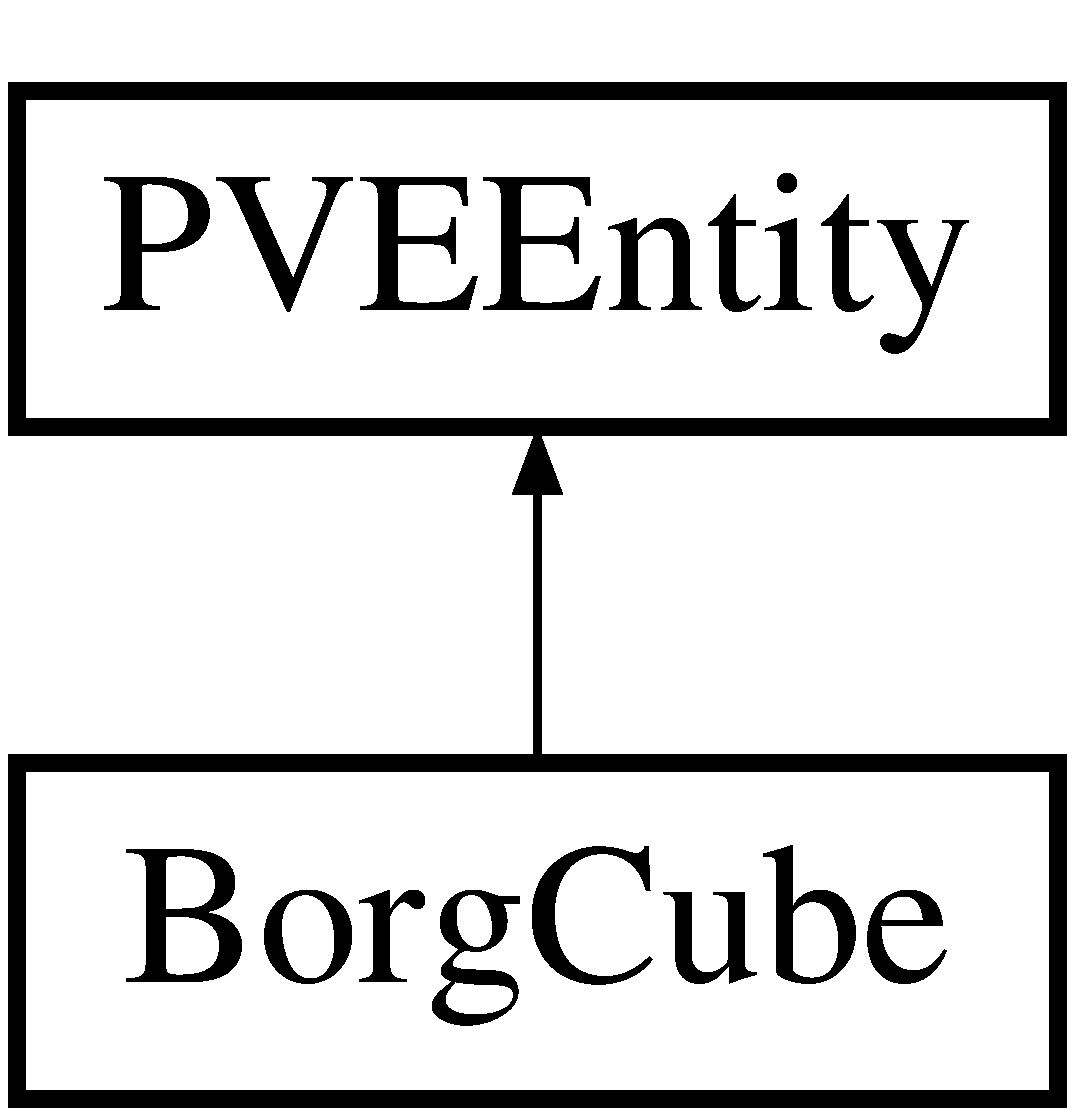
\includegraphics[height=2cm]{d2/d93/classBorgCube}
\end{center}
\end{figure}
\subsection*{Public Member Functions}
\begin{DoxyCompactItemize}
\item 
\hyperlink{classBorgCube_a55a4e4bb838f002a5d83e99519ad22df}{BorgCube} ()
\item 
\hyperlink{classBorgCube_ac714320be9e02beb96853f7143a71486}{$\sim$BorgCube} ()
\item 
string \hyperlink{classBorgCube_a55fa0b12833f3df64b8157c2c05a2bfe}{getName} ()
\item 
int \hyperlink{classBorgCube_a7a6144a9e194eaccdf5d24965b12903c}{getShieldStrenght} ()
\item 
int \hyperlink{classBorgCube_a81acc970f271200df76d98f963c2de75}{getShieldRegenerativeRate} ()
\item 
int \hyperlink{classBorgCube_ab69b67f5b39c837efedad33fb7d21c73}{getRegenerativeAdaptivePlating} ()
\item 
bool \hyperlink{classBorgCube_abd8457ff37b980ca21e58dee957046cb}{getHasRegenerativeAdaptivePlating} ()
\item 
int \hyperlink{classBorgCube_a07417d4ed25e0d0efce29f3b5796dbc3}{getTransPhasicTorpedos} ()
\item 
bool \hyperlink{classBorgCube_a043284f5d42efc224320284a74270836}{getHasTransphasicTorpedos} ()
\item 
int \hyperlink{classBorgCube_a46efbcd3dfc7483c0373bf23d94179ba}{getChronitonTorpedos} ()
\item 
bool \hyperlink{classBorgCube_aea74a439176f217e25c9fb37015b9088}{getHasChronitonTorpedos} ()
\item 
int \hyperlink{classBorgCube_adf64a078b71330e27fe3074c5a278428}{getGravimetricTorpedos} ()
\item 
bool \hyperlink{classBorgCube_abb0288f7ec08d8acb2aa0f3be2e4ada4}{getHasGravimetricTorpedos} ()
\item 
int \hyperlink{classBorgCube_aad53d42f485e62d282e3607ce7c33007}{getSpatialTorpedos} ()
\item 
bool \hyperlink{classBorgCube_afdc5573e2b59fd647f4b2ddb67913c43}{getHasSpatialTorpedos} ()
\item 
bool \hyperlink{classBorgCube_a780ad07deecda3bb7a97ed62365b926f}{getHasLasers} ()
\item 
bool \hyperlink{classBorgCube_af7010edc4afc7ab22fe8bc8294156478}{getHasPhasedIonCannon} ()
\item 
bool \hyperlink{classBorgCube_aff18909b84ec3efb8aa26b6a3aa6cba0}{getHasPulseWeapon} ()
\item 
int \hyperlink{classBorgCube_a971df059540d40c2fbf69116c6ea991f}{getBorgComplement} ()
\item 
bool \hyperlink{classBorgCube_a9090916676b96c967245603216470be6}{getHasTractorLock} ()
\item 
bool \hyperlink{classBorgCube_ad1da81322c189f42505e3ee135be7289}{getIsWreckPVE} ()
\item 
void \hyperlink{classBorgCube_a4590ecc3b6fa8c5f4051a7d1f58c81a2}{setShieldStrenghtPVE} (int strenght)
\item 
void \hyperlink{classBorgCube_ac7dd191ef58188f716cce88130225e19}{setShieldRegenerativeRatePVE} (int rate)
\item 
void \hyperlink{classBorgCube_acf52ecf22eced30bb13babcf67834c6a}{setArmourPVE} (int armour)
\item 
void \hyperlink{classBorgCube_a57d56e4d39de504354dd318a23f7dab7}{setTransPhasicTorpedosPVE} (int num)
\item 
void \hyperlink{classBorgCube_a1a4a73eb1b38f0d8b79445d8e4be691f}{setChronitonTorpedosPVE} (int num)
\item 
void \hyperlink{classBorgCube_a58c2c36486db382f82ab33fcd3c16937}{setGravimetricTorpedosPVE} (int num)
\item 
void \hyperlink{classBorgCube_a98ae970219c8449220e3fac00456775d}{setSpatialTorpedosPVE} (int num)
\item 
void \hyperlink{classBorgCube_ada98eeae90c300a04e787209bb8611df}{setHasTractorLockPVE} (bool has)
\item 
void \hyperlink{classBorgCube_ad764e3b9b70804c7cb2f292628fcf7fd}{setWreckPVE} ()
\end{DoxyCompactItemize}


\subsection{Constructor \& Destructor Documentation}
\hypertarget{classBorgCube_a55a4e4bb838f002a5d83e99519ad22df}{
\index{BorgCube@{BorgCube}!BorgCube@{BorgCube}}
\index{BorgCube@{BorgCube}!BorgCube@{BorgCube}}
\subsubsection[{BorgCube}]{\setlength{\rightskip}{0pt plus 5cm}BorgCube::BorgCube ()}}
\label{d2/d93/classBorgCube_a55a4e4bb838f002a5d83e99519ad22df}
Constructor for pve entity sets up data embers based on preloaded variables arrays usning random index \hypertarget{classBorgCube_ac714320be9e02beb96853f7143a71486}{
\index{BorgCube@{BorgCube}!$\sim$BorgCube@{$\sim$BorgCube}}
\index{$\sim$BorgCube@{$\sim$BorgCube}!BorgCube@{BorgCube}}
\subsubsection[{$\sim$BorgCube}]{\setlength{\rightskip}{0pt plus 5cm}BorgCube::$\sim$BorgCube ()}}
\label{d2/d93/classBorgCube_ac714320be9e02beb96853f7143a71486}
Destructor for the enemy 

\subsection{Member Function Documentation}
\hypertarget{classBorgCube_a971df059540d40c2fbf69116c6ea991f}{
\index{BorgCube@{BorgCube}!getBorgComplement@{getBorgComplement}}
\index{getBorgComplement@{getBorgComplement}!BorgCube@{BorgCube}}
\subsubsection[{getBorgComplement}]{\setlength{\rightskip}{0pt plus 5cm}int BorgCube::getBorgComplement ()\hspace{0.3cm}{\ttfamily  \mbox{[}virtual\mbox{]}}}}
\label{d2/d93/classBorgCube_a971df059540d40c2fbf69116c6ea991f}
accessor for the enemies borg complement

\begin{DoxyReturn}{Returns}
int the borg complement data member 
\end{DoxyReturn}


Implements \hyperlink{classPVEEntity}{PVEEntity}.

\hypertarget{classBorgCube_a46efbcd3dfc7483c0373bf23d94179ba}{
\index{BorgCube@{BorgCube}!getChronitonTorpedos@{getChronitonTorpedos}}
\index{getChronitonTorpedos@{getChronitonTorpedos}!BorgCube@{BorgCube}}
\subsubsection[{getChronitonTorpedos}]{\setlength{\rightskip}{0pt plus 5cm}int BorgCube::getChronitonTorpedos ()\hspace{0.3cm}{\ttfamily  \mbox{[}virtual\mbox{]}}}}
\label{d2/d93/classBorgCube_a46efbcd3dfc7483c0373bf23d94179ba}
accessor for the enemies chroniton torps

\begin{DoxyReturn}{Returns}
int the chroniton torps data member 
\end{DoxyReturn}


Implements \hyperlink{classPVEEntity}{PVEEntity}.

\hypertarget{classBorgCube_adf64a078b71330e27fe3074c5a278428}{
\index{BorgCube@{BorgCube}!getGravimetricTorpedos@{getGravimetricTorpedos}}
\index{getGravimetricTorpedos@{getGravimetricTorpedos}!BorgCube@{BorgCube}}
\subsubsection[{getGravimetricTorpedos}]{\setlength{\rightskip}{0pt plus 5cm}int BorgCube::getGravimetricTorpedos ()\hspace{0.3cm}{\ttfamily  \mbox{[}virtual\mbox{]}}}}
\label{d2/d93/classBorgCube_adf64a078b71330e27fe3074c5a278428}
accessor for the enemies gravimetric torps

\begin{DoxyReturn}{Returns}
int the chroniton torps data member 
\end{DoxyReturn}


Implements \hyperlink{classPVEEntity}{PVEEntity}.

\hypertarget{classBorgCube_aea74a439176f217e25c9fb37015b9088}{
\index{BorgCube@{BorgCube}!getHasChronitonTorpedos@{getHasChronitonTorpedos}}
\index{getHasChronitonTorpedos@{getHasChronitonTorpedos}!BorgCube@{BorgCube}}
\subsubsection[{getHasChronitonTorpedos}]{\setlength{\rightskip}{0pt plus 5cm}bool BorgCube::getHasChronitonTorpedos ()\hspace{0.3cm}{\ttfamily  \mbox{[}virtual\mbox{]}}}}
\label{d2/d93/classBorgCube_aea74a439176f217e25c9fb37015b9088}
accessor for the enemies has chroniton torps

\begin{DoxyReturn}{Returns}
bool the has chroniton torps data member 
\end{DoxyReturn}


Implements \hyperlink{classPVEEntity}{PVEEntity}.

\hypertarget{classBorgCube_abb0288f7ec08d8acb2aa0f3be2e4ada4}{
\index{BorgCube@{BorgCube}!getHasGravimetricTorpedos@{getHasGravimetricTorpedos}}
\index{getHasGravimetricTorpedos@{getHasGravimetricTorpedos}!BorgCube@{BorgCube}}
\subsubsection[{getHasGravimetricTorpedos}]{\setlength{\rightskip}{0pt plus 5cm}bool BorgCube::getHasGravimetricTorpedos ()\hspace{0.3cm}{\ttfamily  \mbox{[}virtual\mbox{]}}}}
\label{d2/d93/classBorgCube_abb0288f7ec08d8acb2aa0f3be2e4ada4}
accessor for the enemies has gravimetric torps

\begin{DoxyReturn}{Returns}
bool the has chroniton torps data member 
\end{DoxyReturn}


Implements \hyperlink{classPVEEntity}{PVEEntity}.

\hypertarget{classBorgCube_a780ad07deecda3bb7a97ed62365b926f}{
\index{BorgCube@{BorgCube}!getHasLasers@{getHasLasers}}
\index{getHasLasers@{getHasLasers}!BorgCube@{BorgCube}}
\subsubsection[{getHasLasers}]{\setlength{\rightskip}{0pt plus 5cm}bool BorgCube::getHasLasers ()\hspace{0.3cm}{\ttfamily  \mbox{[}virtual\mbox{]}}}}
\label{d2/d93/classBorgCube_a780ad07deecda3bb7a97ed62365b926f}
accessor for the enemies has lasers

\begin{DoxyReturn}{Returns}
bool the has lasers data member 
\end{DoxyReturn}


Implements \hyperlink{classPVEEntity}{PVEEntity}.

\hypertarget{classBorgCube_af7010edc4afc7ab22fe8bc8294156478}{
\index{BorgCube@{BorgCube}!getHasPhasedIonCannon@{getHasPhasedIonCannon}}
\index{getHasPhasedIonCannon@{getHasPhasedIonCannon}!BorgCube@{BorgCube}}
\subsubsection[{getHasPhasedIonCannon}]{\setlength{\rightskip}{0pt plus 5cm}bool BorgCube::getHasPhasedIonCannon ()\hspace{0.3cm}{\ttfamily  \mbox{[}virtual\mbox{]}}}}
\label{d2/d93/classBorgCube_af7010edc4afc7ab22fe8bc8294156478}
accessor for the enemies has phased ion cannon

\begin{DoxyReturn}{Returns}
bool the has phased ion cannon data member 
\end{DoxyReturn}


Implements \hyperlink{classPVEEntity}{PVEEntity}.

\hypertarget{classBorgCube_aff18909b84ec3efb8aa26b6a3aa6cba0}{
\index{BorgCube@{BorgCube}!getHasPulseWeapon@{getHasPulseWeapon}}
\index{getHasPulseWeapon@{getHasPulseWeapon}!BorgCube@{BorgCube}}
\subsubsection[{getHasPulseWeapon}]{\setlength{\rightskip}{0pt plus 5cm}bool BorgCube::getHasPulseWeapon ()\hspace{0.3cm}{\ttfamily  \mbox{[}virtual\mbox{]}}}}
\label{d2/d93/classBorgCube_aff18909b84ec3efb8aa26b6a3aa6cba0}
accessor for the enemies has pulse weapons

\begin{DoxyReturn}{Returns}
bool the has pulse weapons data member 
\end{DoxyReturn}


Implements \hyperlink{classPVEEntity}{PVEEntity}.

\hypertarget{classBorgCube_abd8457ff37b980ca21e58dee957046cb}{
\index{BorgCube@{BorgCube}!getHasRegenerativeAdaptivePlating@{getHasRegenerativeAdaptivePlating}}
\index{getHasRegenerativeAdaptivePlating@{getHasRegenerativeAdaptivePlating}!BorgCube@{BorgCube}}
\subsubsection[{getHasRegenerativeAdaptivePlating}]{\setlength{\rightskip}{0pt plus 5cm}bool BorgCube::getHasRegenerativeAdaptivePlating ()\hspace{0.3cm}{\ttfamily  \mbox{[}virtual\mbox{]}}}}
\label{d2/d93/classBorgCube_abd8457ff37b980ca21e58dee957046cb}
accessor for the enemies has regenerative adaptive plating

\begin{DoxyReturn}{Returns}
bool the has regenerative adaptive plating data member 
\end{DoxyReturn}


Implements \hyperlink{classPVEEntity}{PVEEntity}.

\hypertarget{classBorgCube_afdc5573e2b59fd647f4b2ddb67913c43}{
\index{BorgCube@{BorgCube}!getHasSpatialTorpedos@{getHasSpatialTorpedos}}
\index{getHasSpatialTorpedos@{getHasSpatialTorpedos}!BorgCube@{BorgCube}}
\subsubsection[{getHasSpatialTorpedos}]{\setlength{\rightskip}{0pt plus 5cm}bool BorgCube::getHasSpatialTorpedos ()\hspace{0.3cm}{\ttfamily  \mbox{[}virtual\mbox{]}}}}
\label{d2/d93/classBorgCube_afdc5573e2b59fd647f4b2ddb67913c43}
accessor for the enemies has spatial torps

\begin{DoxyReturn}{Returns}
bool the has spatial torps data member 
\end{DoxyReturn}


Implements \hyperlink{classPVEEntity}{PVEEntity}.

\hypertarget{classBorgCube_a9090916676b96c967245603216470be6}{
\index{BorgCube@{BorgCube}!getHasTractorLock@{getHasTractorLock}}
\index{getHasTractorLock@{getHasTractorLock}!BorgCube@{BorgCube}}
\subsubsection[{getHasTractorLock}]{\setlength{\rightskip}{0pt plus 5cm}bool BorgCube::getHasTractorLock ()\hspace{0.3cm}{\ttfamily  \mbox{[}virtual\mbox{]}}}}
\label{d2/d93/classBorgCube_a9090916676b96c967245603216470be6}
accessor for the enemies tractor lock

\begin{DoxyReturn}{Returns}
bool the tractor lock data member 
\end{DoxyReturn}


Implements \hyperlink{classPVEEntity}{PVEEntity}.

\hypertarget{classBorgCube_a043284f5d42efc224320284a74270836}{
\index{BorgCube@{BorgCube}!getHasTransphasicTorpedos@{getHasTransphasicTorpedos}}
\index{getHasTransphasicTorpedos@{getHasTransphasicTorpedos}!BorgCube@{BorgCube}}
\subsubsection[{getHasTransphasicTorpedos}]{\setlength{\rightskip}{0pt plus 5cm}bool BorgCube::getHasTransphasicTorpedos ()\hspace{0.3cm}{\ttfamily  \mbox{[}virtual\mbox{]}}}}
\label{d2/d93/classBorgCube_a043284f5d42efc224320284a74270836}
accessor for the enemies has transphasic torps

\begin{DoxyReturn}{Returns}
bool the has transphasic torps data member 
\end{DoxyReturn}


Implements \hyperlink{classPVEEntity}{PVEEntity}.

\hypertarget{classBorgCube_ad1da81322c189f42505e3ee135be7289}{
\index{BorgCube@{BorgCube}!getIsWreckPVE@{getIsWreckPVE}}
\index{getIsWreckPVE@{getIsWreckPVE}!BorgCube@{BorgCube}}
\subsubsection[{getIsWreckPVE}]{\setlength{\rightskip}{0pt plus 5cm}bool BorgCube::getIsWreckPVE ()\hspace{0.3cm}{\ttfamily  \mbox{[}virtual\mbox{]}}}}
\label{d2/d93/classBorgCube_ad1da81322c189f42505e3ee135be7289}
accessor for the enemies wreck status

\begin{DoxyReturn}{Returns}
bool the wreck status data member 
\end{DoxyReturn}


Implements \hyperlink{classPVEEntity}{PVEEntity}.

\hypertarget{classBorgCube_a55fa0b12833f3df64b8157c2c05a2bfe}{
\index{BorgCube@{BorgCube}!getName@{getName}}
\index{getName@{getName}!BorgCube@{BorgCube}}
\subsubsection[{getName}]{\setlength{\rightskip}{0pt plus 5cm}string BorgCube::getName ()\hspace{0.3cm}{\ttfamily  \mbox{[}virtual\mbox{]}}}}
\label{d2/d93/classBorgCube_a55fa0b12833f3df64b8157c2c05a2bfe}
accessor for the enemies name

\begin{DoxyReturn}{Returns}
string the enemies name 
\end{DoxyReturn}


Implements \hyperlink{classPVEEntity}{PVEEntity}.

\hypertarget{classBorgCube_ab69b67f5b39c837efedad33fb7d21c73}{
\index{BorgCube@{BorgCube}!getRegenerativeAdaptivePlating@{getRegenerativeAdaptivePlating}}
\index{getRegenerativeAdaptivePlating@{getRegenerativeAdaptivePlating}!BorgCube@{BorgCube}}
\subsubsection[{getRegenerativeAdaptivePlating}]{\setlength{\rightskip}{0pt plus 5cm}int BorgCube::getRegenerativeAdaptivePlating ()\hspace{0.3cm}{\ttfamily  \mbox{[}virtual\mbox{]}}}}
\label{d2/d93/classBorgCube_ab69b67f5b39c837efedad33fb7d21c73}
accessor for the enemies regenerative adaptive plating

\begin{DoxyReturn}{Returns}
int the regenerative adaptive plating data member 
\end{DoxyReturn}


Implements \hyperlink{classPVEEntity}{PVEEntity}.

\hypertarget{classBorgCube_a81acc970f271200df76d98f963c2de75}{
\index{BorgCube@{BorgCube}!getShieldRegenerativeRate@{getShieldRegenerativeRate}}
\index{getShieldRegenerativeRate@{getShieldRegenerativeRate}!BorgCube@{BorgCube}}
\subsubsection[{getShieldRegenerativeRate}]{\setlength{\rightskip}{0pt plus 5cm}int BorgCube::getShieldRegenerativeRate ()\hspace{0.3cm}{\ttfamily  \mbox{[}virtual\mbox{]}}}}
\label{d2/d93/classBorgCube_a81acc970f271200df76d98f963c2de75}
accessor for the enemies shield regenerative rate

\begin{DoxyReturn}{Returns}
int the shield regenerative rate data member 
\end{DoxyReturn}


Implements \hyperlink{classPVEEntity}{PVEEntity}.

\hypertarget{classBorgCube_a7a6144a9e194eaccdf5d24965b12903c}{
\index{BorgCube@{BorgCube}!getShieldStrenght@{getShieldStrenght}}
\index{getShieldStrenght@{getShieldStrenght}!BorgCube@{BorgCube}}
\subsubsection[{getShieldStrenght}]{\setlength{\rightskip}{0pt plus 5cm}int BorgCube::getShieldStrenght ()\hspace{0.3cm}{\ttfamily  \mbox{[}virtual\mbox{]}}}}
\label{d2/d93/classBorgCube_a7a6144a9e194eaccdf5d24965b12903c}
accessor for the enemies shield strength

\begin{DoxyReturn}{Returns}
int the shield strength data member 
\end{DoxyReturn}


Implements \hyperlink{classPVEEntity}{PVEEntity}.

\hypertarget{classBorgCube_aad53d42f485e62d282e3607ce7c33007}{
\index{BorgCube@{BorgCube}!getSpatialTorpedos@{getSpatialTorpedos}}
\index{getSpatialTorpedos@{getSpatialTorpedos}!BorgCube@{BorgCube}}
\subsubsection[{getSpatialTorpedos}]{\setlength{\rightskip}{0pt plus 5cm}int BorgCube::getSpatialTorpedos ()\hspace{0.3cm}{\ttfamily  \mbox{[}virtual\mbox{]}}}}
\label{d2/d93/classBorgCube_aad53d42f485e62d282e3607ce7c33007}
accessor for the enemies spatial torps

\begin{DoxyReturn}{Returns}
int the spatial torps data member 
\end{DoxyReturn}


Implements \hyperlink{classPVEEntity}{PVEEntity}.

\hypertarget{classBorgCube_a07417d4ed25e0d0efce29f3b5796dbc3}{
\index{BorgCube@{BorgCube}!getTransPhasicTorpedos@{getTransPhasicTorpedos}}
\index{getTransPhasicTorpedos@{getTransPhasicTorpedos}!BorgCube@{BorgCube}}
\subsubsection[{getTransPhasicTorpedos}]{\setlength{\rightskip}{0pt plus 5cm}int BorgCube::getTransPhasicTorpedos ()\hspace{0.3cm}{\ttfamily  \mbox{[}virtual\mbox{]}}}}
\label{d2/d93/classBorgCube_a07417d4ed25e0d0efce29f3b5796dbc3}
accessor for the enemies has regenerative adaptive plating

\begin{DoxyReturn}{Returns}
bool the has regenerative adaptive plating data member 
\end{DoxyReturn}


Implements \hyperlink{classPVEEntity}{PVEEntity}.

\hypertarget{classBorgCube_acf52ecf22eced30bb13babcf67834c6a}{
\index{BorgCube@{BorgCube}!setArmourPVE@{setArmourPVE}}
\index{setArmourPVE@{setArmourPVE}!BorgCube@{BorgCube}}
\subsubsection[{setArmourPVE}]{\setlength{\rightskip}{0pt plus 5cm}void BorgCube::setArmourPVE (int {\em armour})\hspace{0.3cm}{\ttfamily  \mbox{[}virtual\mbox{]}}}}
\label{d2/d93/classBorgCube_acf52ecf22eced30bb13babcf67834c6a}
mutator for the enemies armour


\begin{DoxyParams}{Parameters}
\item[{\em armour}]the value to set the data member\end{DoxyParams}
\begin{DoxyReturn}{Returns}
void 
\end{DoxyReturn}


Implements \hyperlink{classPVEEntity}{PVEEntity}.

\hypertarget{classBorgCube_a1a4a73eb1b38f0d8b79445d8e4be691f}{
\index{BorgCube@{BorgCube}!setChronitonTorpedosPVE@{setChronitonTorpedosPVE}}
\index{setChronitonTorpedosPVE@{setChronitonTorpedosPVE}!BorgCube@{BorgCube}}
\subsubsection[{setChronitonTorpedosPVE}]{\setlength{\rightskip}{0pt plus 5cm}void BorgCube::setChronitonTorpedosPVE (int {\em num})\hspace{0.3cm}{\ttfamily  \mbox{[}virtual\mbox{]}}}}
\label{d2/d93/classBorgCube_a1a4a73eb1b38f0d8b79445d8e4be691f}
mutator for the enemies chroniton torps


\begin{DoxyParams}{Parameters}
\item[{\em num}]the value to set the data member\end{DoxyParams}
\begin{DoxyReturn}{Returns}
void 
\end{DoxyReturn}


Implements \hyperlink{classPVEEntity}{PVEEntity}.

\hypertarget{classBorgCube_a58c2c36486db382f82ab33fcd3c16937}{
\index{BorgCube@{BorgCube}!setGravimetricTorpedosPVE@{setGravimetricTorpedosPVE}}
\index{setGravimetricTorpedosPVE@{setGravimetricTorpedosPVE}!BorgCube@{BorgCube}}
\subsubsection[{setGravimetricTorpedosPVE}]{\setlength{\rightskip}{0pt plus 5cm}void BorgCube::setGravimetricTorpedosPVE (int {\em num})\hspace{0.3cm}{\ttfamily  \mbox{[}virtual\mbox{]}}}}
\label{d2/d93/classBorgCube_a58c2c36486db382f82ab33fcd3c16937}
mutator for the enemies gravimetric torps


\begin{DoxyParams}{Parameters}
\item[{\em num}]the value to set the data member\end{DoxyParams}
\begin{DoxyReturn}{Returns}
void 
\end{DoxyReturn}


Implements \hyperlink{classPVEEntity}{PVEEntity}.

\hypertarget{classBorgCube_ada98eeae90c300a04e787209bb8611df}{
\index{BorgCube@{BorgCube}!setHasTractorLockPVE@{setHasTractorLockPVE}}
\index{setHasTractorLockPVE@{setHasTractorLockPVE}!BorgCube@{BorgCube}}
\subsubsection[{setHasTractorLockPVE}]{\setlength{\rightskip}{0pt plus 5cm}void BorgCube::setHasTractorLockPVE (bool {\em has})\hspace{0.3cm}{\ttfamily  \mbox{[}virtual\mbox{]}}}}
\label{d2/d93/classBorgCube_ada98eeae90c300a04e787209bb8611df}
mutator for the enemies tractor beam


\begin{DoxyParams}{Parameters}
\item[{\em has}]the bool value to set the data member\end{DoxyParams}
\begin{DoxyReturn}{Returns}
void 
\end{DoxyReturn}


Implements \hyperlink{classPVEEntity}{PVEEntity}.

\hypertarget{classBorgCube_ac7dd191ef58188f716cce88130225e19}{
\index{BorgCube@{BorgCube}!setShieldRegenerativeRatePVE@{setShieldRegenerativeRatePVE}}
\index{setShieldRegenerativeRatePVE@{setShieldRegenerativeRatePVE}!BorgCube@{BorgCube}}
\subsubsection[{setShieldRegenerativeRatePVE}]{\setlength{\rightskip}{0pt plus 5cm}void BorgCube::setShieldRegenerativeRatePVE (int {\em rate})\hspace{0.3cm}{\ttfamily  \mbox{[}virtual\mbox{]}}}}
\label{d2/d93/classBorgCube_ac7dd191ef58188f716cce88130225e19}
mutator for the enemies regenerative rate


\begin{DoxyParams}{Parameters}
\item[{\em rate}]the value to set the data member\end{DoxyParams}
\begin{DoxyReturn}{Returns}
void 
\end{DoxyReturn}


Implements \hyperlink{classPVEEntity}{PVEEntity}.

\hypertarget{classBorgCube_a4590ecc3b6fa8c5f4051a7d1f58c81a2}{
\index{BorgCube@{BorgCube}!setShieldStrenghtPVE@{setShieldStrenghtPVE}}
\index{setShieldStrenghtPVE@{setShieldStrenghtPVE}!BorgCube@{BorgCube}}
\subsubsection[{setShieldStrenghtPVE}]{\setlength{\rightskip}{0pt plus 5cm}void BorgCube::setShieldStrenghtPVE (int {\em strenght})\hspace{0.3cm}{\ttfamily  \mbox{[}virtual\mbox{]}}}}
\label{d2/d93/classBorgCube_a4590ecc3b6fa8c5f4051a7d1f58c81a2}
mutator for the enemies shield strength


\begin{DoxyParams}{Parameters}
\item[{\em strenght}]the value to set the data member\end{DoxyParams}
\begin{DoxyReturn}{Returns}
void 
\end{DoxyReturn}


Implements \hyperlink{classPVEEntity}{PVEEntity}.

\hypertarget{classBorgCube_a98ae970219c8449220e3fac00456775d}{
\index{BorgCube@{BorgCube}!setSpatialTorpedosPVE@{setSpatialTorpedosPVE}}
\index{setSpatialTorpedosPVE@{setSpatialTorpedosPVE}!BorgCube@{BorgCube}}
\subsubsection[{setSpatialTorpedosPVE}]{\setlength{\rightskip}{0pt plus 5cm}void BorgCube::setSpatialTorpedosPVE (int {\em num})\hspace{0.3cm}{\ttfamily  \mbox{[}virtual\mbox{]}}}}
\label{d2/d93/classBorgCube_a98ae970219c8449220e3fac00456775d}
mutator for the enemies spatial torps


\begin{DoxyParams}{Parameters}
\item[{\em num}]the value to set the data member\end{DoxyParams}
\begin{DoxyReturn}{Returns}
void 
\end{DoxyReturn}


Implements \hyperlink{classPVEEntity}{PVEEntity}.

\hypertarget{classBorgCube_a57d56e4d39de504354dd318a23f7dab7}{
\index{BorgCube@{BorgCube}!setTransPhasicTorpedosPVE@{setTransPhasicTorpedosPVE}}
\index{setTransPhasicTorpedosPVE@{setTransPhasicTorpedosPVE}!BorgCube@{BorgCube}}
\subsubsection[{setTransPhasicTorpedosPVE}]{\setlength{\rightskip}{0pt plus 5cm}void BorgCube::setTransPhasicTorpedosPVE (int {\em num})\hspace{0.3cm}{\ttfamily  \mbox{[}virtual\mbox{]}}}}
\label{d2/d93/classBorgCube_a57d56e4d39de504354dd318a23f7dab7}
mutator for the enemies trans phasic torps


\begin{DoxyParams}{Parameters}
\item[{\em num}]the value to set the data member\end{DoxyParams}
\begin{DoxyReturn}{Returns}
void 
\end{DoxyReturn}


Implements \hyperlink{classPVEEntity}{PVEEntity}.

\hypertarget{classBorgCube_ad764e3b9b70804c7cb2f292628fcf7fd}{
\index{BorgCube@{BorgCube}!setWreckPVE@{setWreckPVE}}
\index{setWreckPVE@{setWreckPVE}!BorgCube@{BorgCube}}
\subsubsection[{setWreckPVE}]{\setlength{\rightskip}{0pt plus 5cm}void BorgCube::setWreckPVE ()\hspace{0.3cm}{\ttfamily  \mbox{[}virtual\mbox{]}}}}
\label{d2/d93/classBorgCube_ad764e3b9b70804c7cb2f292628fcf7fd}
mutator for the enemies wreck state

\begin{DoxyReturn}{Returns}
void 
\end{DoxyReturn}


Implements \hyperlink{classPVEEntity}{PVEEntity}.



The documentation for this class was generated from the following files:\begin{DoxyCompactItemize}
\item 
source/header/BorgCube.h\item 
source/source/BorgCube.cpp\end{DoxyCompactItemize}

\hypertarget{classBorgProbe}{
\section{BorgProbe Class Reference}
\label{db/deb/classBorgProbe}\index{BorgProbe@{BorgProbe}}
}
Inheritance diagram for BorgProbe:\begin{figure}[H]
\begin{center}
\leavevmode
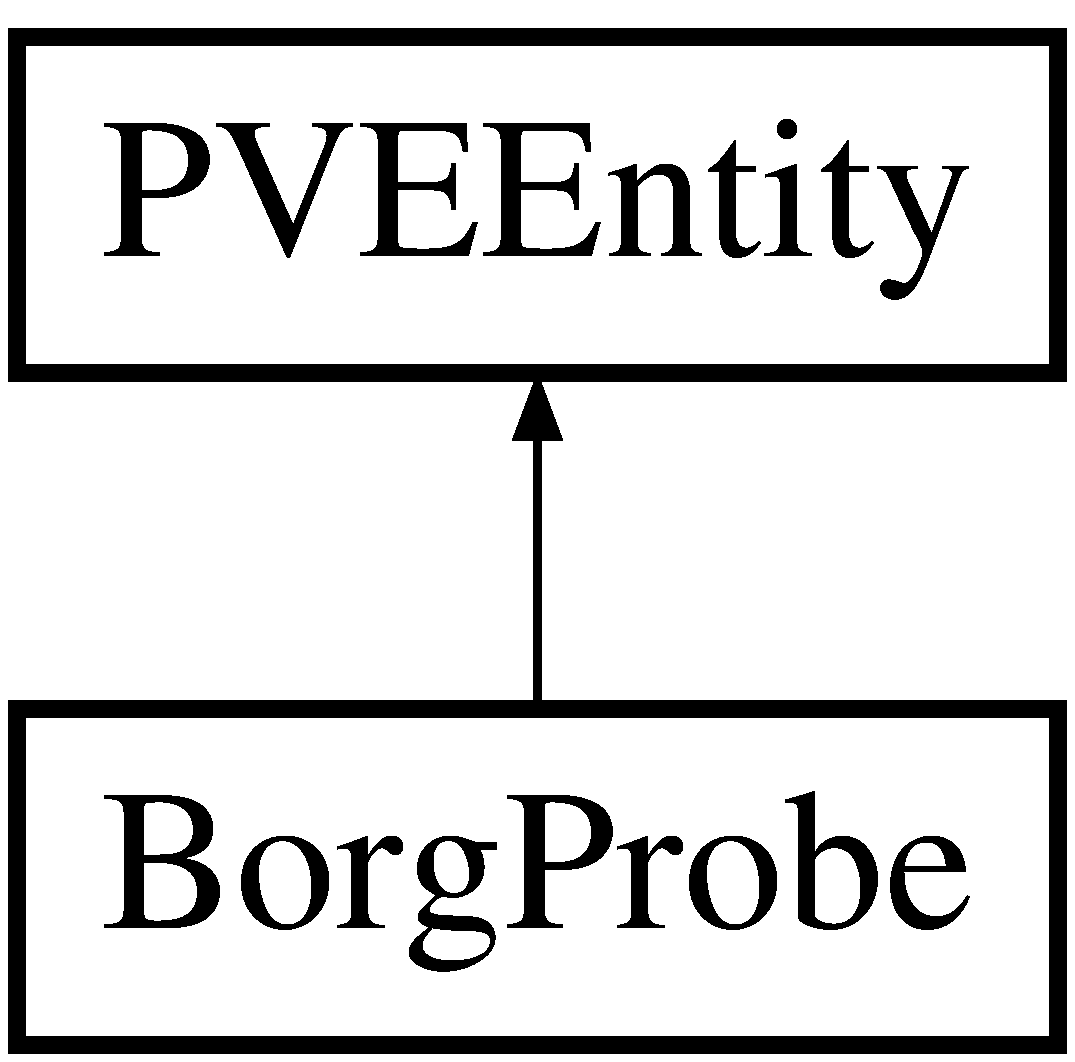
\includegraphics[height=2cm]{db/deb/classBorgProbe}
\end{center}
\end{figure}
\subsection*{Public Member Functions}
\begin{DoxyCompactItemize}
\item 
\hyperlink{classBorgProbe_a3af24a2d8ca19a3770f15a1c873709cb}{BorgProbe} ()
\item 
\hyperlink{classBorgProbe_a4d58be5de785e9816f5c9bbda8625951}{$\sim$BorgProbe} ()
\item 
string \hyperlink{classBorgProbe_a93662b939b7b3565c72445f75c56c101}{getName} ()
\item 
int \hyperlink{classBorgProbe_a06fb45579883333083eda36335ef7349}{getShieldStrenght} ()
\item 
int \hyperlink{classBorgProbe_a0bd8db46345776e54af6c198fb4a5c3b}{getShieldRegenerativeRate} ()
\item 
int \hyperlink{classBorgProbe_ab2bd1c4edaae54e53ebec17b4680b11b}{getRegenerativeAdaptivePlating} ()
\item 
bool \hyperlink{classBorgProbe_a5c21dac867e41d71305cce22f6519586}{getHasRegenerativeAdaptivePlating} ()
\item 
int \hyperlink{classBorgProbe_a1879936ef2e6dec0df73dc2628055be7}{getTransPhasicTorpedos} ()
\item 
bool \hyperlink{classBorgProbe_a304d8f8cc7fb8f1d47ab5edf6fe02ba6}{getHasTransphasicTorpedos} ()
\item 
int \hyperlink{classBorgProbe_a4eec0f21a2a68a57498aef50d4d7c544}{getChronitonTorpedos} ()
\item 
bool \hyperlink{classBorgProbe_a6edb033d9ace089d17c1495447e76b1d}{getHasChronitonTorpedos} ()
\item 
int \hyperlink{classBorgProbe_aba5ca1bcf4d4f3f37d80b46bb6b40492}{getGravimetricTorpedos} ()
\item 
bool \hyperlink{classBorgProbe_a882991a84e51a0fd78de0320d4bec53a}{getHasGravimetricTorpedos} ()
\item 
int \hyperlink{classBorgProbe_aaa3c141850bd6d15e6d8eab68d75583c}{getSpatialTorpedos} ()
\item 
bool \hyperlink{classBorgProbe_afefc3c2911ff75c7d02a8fd4390a9bfd}{getHasSpatialTorpedos} ()
\item 
bool \hyperlink{classBorgProbe_a1a77fe640dd80aa9dd6ceb3b8e9555bf}{getHasLasers} ()
\item 
bool \hyperlink{classBorgProbe_a45245995e7fe90e03f64f63c999339b5}{getHasPhasedIonCannon} ()
\item 
bool \hyperlink{classBorgProbe_a60085d6bf6d31b28bfb60eeedca1c711}{getHasPulseWeapon} ()
\item 
int \hyperlink{classBorgProbe_a4a9d5108f208dcaa28b3f182436fd6e1}{getBorgComplement} ()
\item 
bool \hyperlink{classBorgProbe_a3e0cfde0db3e63c1405afe14699b3122}{getHasTractorLock} ()
\item 
bool \hyperlink{classBorgProbe_ab3a53f7518386129055fa678d75f99a5}{getIsWreckPVE} ()
\item 
void \hyperlink{classBorgProbe_a1866290e2fb1a65e12d4448bcba5d932}{setShieldStrenghtPVE} (int strenght)
\item 
void \hyperlink{classBorgProbe_a6cdeb57ba40d96381f4178d01e3d4cae}{setShieldRegenerativeRatePVE} (int rate)
\item 
void \hyperlink{classBorgProbe_aa823f6c8ba0b31727124e104f2e9956b}{setArmourPVE} (int armour)
\item 
void \hyperlink{classBorgProbe_ade7cc51b7c80a763a1f6c28e0770266e}{setTransPhasicTorpedosPVE} (int num)
\item 
void \hyperlink{classBorgProbe_a8c289005635315de539283a12f96d03e}{setChronitonTorpedosPVE} (int num)
\item 
void \hyperlink{classBorgProbe_a992e10da14904a7ab14bc34ac9ec63ee}{setGravimetricTorpedosPVE} (int num)
\item 
void \hyperlink{classBorgProbe_a69c828eb05d8d652d66b57e12caa96fd}{setSpatialTorpedosPVE} (int num)
\item 
void \hyperlink{classBorgProbe_ab38152299b9d34950bf4acd740544328}{setHasTractorLockPVE} (bool has)
\item 
void \hyperlink{classBorgProbe_a6b4c0d1bdfc717349fd1e74ac710a7da}{setWreckPVE} ()
\end{DoxyCompactItemize}


\subsection{Constructor \& Destructor Documentation}
\hypertarget{classBorgProbe_a3af24a2d8ca19a3770f15a1c873709cb}{
\index{BorgProbe@{BorgProbe}!BorgProbe@{BorgProbe}}
\index{BorgProbe@{BorgProbe}!BorgProbe@{BorgProbe}}
\subsubsection[{BorgProbe}]{\setlength{\rightskip}{0pt plus 5cm}BorgProbe::BorgProbe ()}}
\label{db/deb/classBorgProbe_a3af24a2d8ca19a3770f15a1c873709cb}
Constructor for pve entity sets up data embers based on preloaded variables arrays usning random index \hypertarget{classBorgProbe_a4d58be5de785e9816f5c9bbda8625951}{
\index{BorgProbe@{BorgProbe}!$\sim$BorgProbe@{$\sim$BorgProbe}}
\index{$\sim$BorgProbe@{$\sim$BorgProbe}!BorgProbe@{BorgProbe}}
\subsubsection[{$\sim$BorgProbe}]{\setlength{\rightskip}{0pt plus 5cm}BorgProbe::$\sim$BorgProbe ()}}
\label{db/deb/classBorgProbe_a4d58be5de785e9816f5c9bbda8625951}
Destructor for the enemy 

\subsection{Member Function Documentation}
\hypertarget{classBorgProbe_a4a9d5108f208dcaa28b3f182436fd6e1}{
\index{BorgProbe@{BorgProbe}!getBorgComplement@{getBorgComplement}}
\index{getBorgComplement@{getBorgComplement}!BorgProbe@{BorgProbe}}
\subsubsection[{getBorgComplement}]{\setlength{\rightskip}{0pt plus 5cm}int BorgProbe::getBorgComplement ()\hspace{0.3cm}{\ttfamily  \mbox{[}virtual\mbox{]}}}}
\label{db/deb/classBorgProbe_a4a9d5108f208dcaa28b3f182436fd6e1}
accessor for the enemies borg complement

\begin{DoxyReturn}{Returns}
int the borg complement data member 
\end{DoxyReturn}


Implements \hyperlink{classPVEEntity}{PVEEntity}.

\hypertarget{classBorgProbe_a4eec0f21a2a68a57498aef50d4d7c544}{
\index{BorgProbe@{BorgProbe}!getChronitonTorpedos@{getChronitonTorpedos}}
\index{getChronitonTorpedos@{getChronitonTorpedos}!BorgProbe@{BorgProbe}}
\subsubsection[{getChronitonTorpedos}]{\setlength{\rightskip}{0pt plus 5cm}int BorgProbe::getChronitonTorpedos ()\hspace{0.3cm}{\ttfamily  \mbox{[}virtual\mbox{]}}}}
\label{db/deb/classBorgProbe_a4eec0f21a2a68a57498aef50d4d7c544}
accessor for the enemies chroniton torps

\begin{DoxyReturn}{Returns}
int the chroniton torps data member 
\end{DoxyReturn}


Implements \hyperlink{classPVEEntity}{PVEEntity}.

\hypertarget{classBorgProbe_aba5ca1bcf4d4f3f37d80b46bb6b40492}{
\index{BorgProbe@{BorgProbe}!getGravimetricTorpedos@{getGravimetricTorpedos}}
\index{getGravimetricTorpedos@{getGravimetricTorpedos}!BorgProbe@{BorgProbe}}
\subsubsection[{getGravimetricTorpedos}]{\setlength{\rightskip}{0pt plus 5cm}int BorgProbe::getGravimetricTorpedos ()\hspace{0.3cm}{\ttfamily  \mbox{[}virtual\mbox{]}}}}
\label{db/deb/classBorgProbe_aba5ca1bcf4d4f3f37d80b46bb6b40492}
accessor for the enemies gravimetric torps

\begin{DoxyReturn}{Returns}
int the chroniton torps data member 
\end{DoxyReturn}


Implements \hyperlink{classPVEEntity}{PVEEntity}.

\hypertarget{classBorgProbe_a6edb033d9ace089d17c1495447e76b1d}{
\index{BorgProbe@{BorgProbe}!getHasChronitonTorpedos@{getHasChronitonTorpedos}}
\index{getHasChronitonTorpedos@{getHasChronitonTorpedos}!BorgProbe@{BorgProbe}}
\subsubsection[{getHasChronitonTorpedos}]{\setlength{\rightskip}{0pt plus 5cm}bool BorgProbe::getHasChronitonTorpedos ()\hspace{0.3cm}{\ttfamily  \mbox{[}virtual\mbox{]}}}}
\label{db/deb/classBorgProbe_a6edb033d9ace089d17c1495447e76b1d}
accessor for the enemies has chroniton torps

\begin{DoxyReturn}{Returns}
bool the has chroniton torps data member 
\end{DoxyReturn}


Implements \hyperlink{classPVEEntity}{PVEEntity}.

\hypertarget{classBorgProbe_a882991a84e51a0fd78de0320d4bec53a}{
\index{BorgProbe@{BorgProbe}!getHasGravimetricTorpedos@{getHasGravimetricTorpedos}}
\index{getHasGravimetricTorpedos@{getHasGravimetricTorpedos}!BorgProbe@{BorgProbe}}
\subsubsection[{getHasGravimetricTorpedos}]{\setlength{\rightskip}{0pt plus 5cm}bool BorgProbe::getHasGravimetricTorpedos ()\hspace{0.3cm}{\ttfamily  \mbox{[}virtual\mbox{]}}}}
\label{db/deb/classBorgProbe_a882991a84e51a0fd78de0320d4bec53a}
accessor for the enemies has gravimetric torps

\begin{DoxyReturn}{Returns}
bool the has chroniton torps data member 
\end{DoxyReturn}


Implements \hyperlink{classPVEEntity}{PVEEntity}.

\hypertarget{classBorgProbe_a1a77fe640dd80aa9dd6ceb3b8e9555bf}{
\index{BorgProbe@{BorgProbe}!getHasLasers@{getHasLasers}}
\index{getHasLasers@{getHasLasers}!BorgProbe@{BorgProbe}}
\subsubsection[{getHasLasers}]{\setlength{\rightskip}{0pt plus 5cm}bool BorgProbe::getHasLasers ()\hspace{0.3cm}{\ttfamily  \mbox{[}virtual\mbox{]}}}}
\label{db/deb/classBorgProbe_a1a77fe640dd80aa9dd6ceb3b8e9555bf}
accessor for the enemies has lasers

\begin{DoxyReturn}{Returns}
bool the has lasers data member 
\end{DoxyReturn}


Implements \hyperlink{classPVEEntity}{PVEEntity}.

\hypertarget{classBorgProbe_a45245995e7fe90e03f64f63c999339b5}{
\index{BorgProbe@{BorgProbe}!getHasPhasedIonCannon@{getHasPhasedIonCannon}}
\index{getHasPhasedIonCannon@{getHasPhasedIonCannon}!BorgProbe@{BorgProbe}}
\subsubsection[{getHasPhasedIonCannon}]{\setlength{\rightskip}{0pt plus 5cm}bool BorgProbe::getHasPhasedIonCannon ()\hspace{0.3cm}{\ttfamily  \mbox{[}virtual\mbox{]}}}}
\label{db/deb/classBorgProbe_a45245995e7fe90e03f64f63c999339b5}
accessor for the enemies has phased ion cannon

\begin{DoxyReturn}{Returns}
bool the has phased ion cannon data member 
\end{DoxyReturn}


Implements \hyperlink{classPVEEntity}{PVEEntity}.

\hypertarget{classBorgProbe_a60085d6bf6d31b28bfb60eeedca1c711}{
\index{BorgProbe@{BorgProbe}!getHasPulseWeapon@{getHasPulseWeapon}}
\index{getHasPulseWeapon@{getHasPulseWeapon}!BorgProbe@{BorgProbe}}
\subsubsection[{getHasPulseWeapon}]{\setlength{\rightskip}{0pt plus 5cm}bool BorgProbe::getHasPulseWeapon ()\hspace{0.3cm}{\ttfamily  \mbox{[}virtual\mbox{]}}}}
\label{db/deb/classBorgProbe_a60085d6bf6d31b28bfb60eeedca1c711}
accessor for the enemies has pulse weapons

\begin{DoxyReturn}{Returns}
bool the has pulse weapons data member 
\end{DoxyReturn}


Implements \hyperlink{classPVEEntity}{PVEEntity}.

\hypertarget{classBorgProbe_a5c21dac867e41d71305cce22f6519586}{
\index{BorgProbe@{BorgProbe}!getHasRegenerativeAdaptivePlating@{getHasRegenerativeAdaptivePlating}}
\index{getHasRegenerativeAdaptivePlating@{getHasRegenerativeAdaptivePlating}!BorgProbe@{BorgProbe}}
\subsubsection[{getHasRegenerativeAdaptivePlating}]{\setlength{\rightskip}{0pt plus 5cm}bool BorgProbe::getHasRegenerativeAdaptivePlating ()\hspace{0.3cm}{\ttfamily  \mbox{[}virtual\mbox{]}}}}
\label{db/deb/classBorgProbe_a5c21dac867e41d71305cce22f6519586}
accessor for the enemies has regenerative adaptive plating

\begin{DoxyReturn}{Returns}
bool the has regenerative adaptive plating data member 
\end{DoxyReturn}


Implements \hyperlink{classPVEEntity}{PVEEntity}.

\hypertarget{classBorgProbe_afefc3c2911ff75c7d02a8fd4390a9bfd}{
\index{BorgProbe@{BorgProbe}!getHasSpatialTorpedos@{getHasSpatialTorpedos}}
\index{getHasSpatialTorpedos@{getHasSpatialTorpedos}!BorgProbe@{BorgProbe}}
\subsubsection[{getHasSpatialTorpedos}]{\setlength{\rightskip}{0pt plus 5cm}bool BorgProbe::getHasSpatialTorpedos ()\hspace{0.3cm}{\ttfamily  \mbox{[}virtual\mbox{]}}}}
\label{db/deb/classBorgProbe_afefc3c2911ff75c7d02a8fd4390a9bfd}
accessor for the enemies has spatial torps

\begin{DoxyReturn}{Returns}
bool the has spatial torps data member 
\end{DoxyReturn}


Implements \hyperlink{classPVEEntity}{PVEEntity}.

\hypertarget{classBorgProbe_a3e0cfde0db3e63c1405afe14699b3122}{
\index{BorgProbe@{BorgProbe}!getHasTractorLock@{getHasTractorLock}}
\index{getHasTractorLock@{getHasTractorLock}!BorgProbe@{BorgProbe}}
\subsubsection[{getHasTractorLock}]{\setlength{\rightskip}{0pt plus 5cm}bool BorgProbe::getHasTractorLock ()\hspace{0.3cm}{\ttfamily  \mbox{[}virtual\mbox{]}}}}
\label{db/deb/classBorgProbe_a3e0cfde0db3e63c1405afe14699b3122}
accessor for the enemies tractor lock

\begin{DoxyReturn}{Returns}
bool the tractor lock data member 
\end{DoxyReturn}


Implements \hyperlink{classPVEEntity}{PVEEntity}.

\hypertarget{classBorgProbe_a304d8f8cc7fb8f1d47ab5edf6fe02ba6}{
\index{BorgProbe@{BorgProbe}!getHasTransphasicTorpedos@{getHasTransphasicTorpedos}}
\index{getHasTransphasicTorpedos@{getHasTransphasicTorpedos}!BorgProbe@{BorgProbe}}
\subsubsection[{getHasTransphasicTorpedos}]{\setlength{\rightskip}{0pt plus 5cm}bool BorgProbe::getHasTransphasicTorpedos ()\hspace{0.3cm}{\ttfamily  \mbox{[}virtual\mbox{]}}}}
\label{db/deb/classBorgProbe_a304d8f8cc7fb8f1d47ab5edf6fe02ba6}
accessor for the enemies has transphasic torps

\begin{DoxyReturn}{Returns}
bool the has transphasic torps data member 
\end{DoxyReturn}


Implements \hyperlink{classPVEEntity}{PVEEntity}.

\hypertarget{classBorgProbe_ab3a53f7518386129055fa678d75f99a5}{
\index{BorgProbe@{BorgProbe}!getIsWreckPVE@{getIsWreckPVE}}
\index{getIsWreckPVE@{getIsWreckPVE}!BorgProbe@{BorgProbe}}
\subsubsection[{getIsWreckPVE}]{\setlength{\rightskip}{0pt plus 5cm}bool BorgProbe::getIsWreckPVE ()\hspace{0.3cm}{\ttfamily  \mbox{[}virtual\mbox{]}}}}
\label{db/deb/classBorgProbe_ab3a53f7518386129055fa678d75f99a5}
accessor for the enemies wreck status

\begin{DoxyReturn}{Returns}
bool the wreck status data member 
\end{DoxyReturn}


Implements \hyperlink{classPVEEntity}{PVEEntity}.

\hypertarget{classBorgProbe_a93662b939b7b3565c72445f75c56c101}{
\index{BorgProbe@{BorgProbe}!getName@{getName}}
\index{getName@{getName}!BorgProbe@{BorgProbe}}
\subsubsection[{getName}]{\setlength{\rightskip}{0pt plus 5cm}string BorgProbe::getName ()\hspace{0.3cm}{\ttfamily  \mbox{[}virtual\mbox{]}}}}
\label{db/deb/classBorgProbe_a93662b939b7b3565c72445f75c56c101}
accessor for the enemies name

\begin{DoxyReturn}{Returns}
string the enemies name 
\end{DoxyReturn}


Implements \hyperlink{classPVEEntity}{PVEEntity}.

\hypertarget{classBorgProbe_ab2bd1c4edaae54e53ebec17b4680b11b}{
\index{BorgProbe@{BorgProbe}!getRegenerativeAdaptivePlating@{getRegenerativeAdaptivePlating}}
\index{getRegenerativeAdaptivePlating@{getRegenerativeAdaptivePlating}!BorgProbe@{BorgProbe}}
\subsubsection[{getRegenerativeAdaptivePlating}]{\setlength{\rightskip}{0pt plus 5cm}int BorgProbe::getRegenerativeAdaptivePlating ()\hspace{0.3cm}{\ttfamily  \mbox{[}virtual\mbox{]}}}}
\label{db/deb/classBorgProbe_ab2bd1c4edaae54e53ebec17b4680b11b}
accessor for the enemies regenerative adaptive plating

\begin{DoxyReturn}{Returns}
int the regenerative adaptive plating data member 
\end{DoxyReturn}


Implements \hyperlink{classPVEEntity}{PVEEntity}.

\hypertarget{classBorgProbe_a0bd8db46345776e54af6c198fb4a5c3b}{
\index{BorgProbe@{BorgProbe}!getShieldRegenerativeRate@{getShieldRegenerativeRate}}
\index{getShieldRegenerativeRate@{getShieldRegenerativeRate}!BorgProbe@{BorgProbe}}
\subsubsection[{getShieldRegenerativeRate}]{\setlength{\rightskip}{0pt plus 5cm}int BorgProbe::getShieldRegenerativeRate ()\hspace{0.3cm}{\ttfamily  \mbox{[}virtual\mbox{]}}}}
\label{db/deb/classBorgProbe_a0bd8db46345776e54af6c198fb4a5c3b}
accessor for the enemies shield regenerative rate

\begin{DoxyReturn}{Returns}
int the shield regenerative rate data member 
\end{DoxyReturn}


Implements \hyperlink{classPVEEntity}{PVEEntity}.

\hypertarget{classBorgProbe_a06fb45579883333083eda36335ef7349}{
\index{BorgProbe@{BorgProbe}!getShieldStrenght@{getShieldStrenght}}
\index{getShieldStrenght@{getShieldStrenght}!BorgProbe@{BorgProbe}}
\subsubsection[{getShieldStrenght}]{\setlength{\rightskip}{0pt plus 5cm}int BorgProbe::getShieldStrenght ()\hspace{0.3cm}{\ttfamily  \mbox{[}virtual\mbox{]}}}}
\label{db/deb/classBorgProbe_a06fb45579883333083eda36335ef7349}
accessor for the enemies shield strength

\begin{DoxyReturn}{Returns}
int the shield strength data member 
\end{DoxyReturn}


Implements \hyperlink{classPVEEntity}{PVEEntity}.

\hypertarget{classBorgProbe_aaa3c141850bd6d15e6d8eab68d75583c}{
\index{BorgProbe@{BorgProbe}!getSpatialTorpedos@{getSpatialTorpedos}}
\index{getSpatialTorpedos@{getSpatialTorpedos}!BorgProbe@{BorgProbe}}
\subsubsection[{getSpatialTorpedos}]{\setlength{\rightskip}{0pt plus 5cm}int BorgProbe::getSpatialTorpedos ()\hspace{0.3cm}{\ttfamily  \mbox{[}virtual\mbox{]}}}}
\label{db/deb/classBorgProbe_aaa3c141850bd6d15e6d8eab68d75583c}
accessor for the enemies spatial torps

\begin{DoxyReturn}{Returns}
int the spatial torps data member 
\end{DoxyReturn}


Implements \hyperlink{classPVEEntity}{PVEEntity}.

\hypertarget{classBorgProbe_a1879936ef2e6dec0df73dc2628055be7}{
\index{BorgProbe@{BorgProbe}!getTransPhasicTorpedos@{getTransPhasicTorpedos}}
\index{getTransPhasicTorpedos@{getTransPhasicTorpedos}!BorgProbe@{BorgProbe}}
\subsubsection[{getTransPhasicTorpedos}]{\setlength{\rightskip}{0pt plus 5cm}int BorgProbe::getTransPhasicTorpedos ()\hspace{0.3cm}{\ttfamily  \mbox{[}virtual\mbox{]}}}}
\label{db/deb/classBorgProbe_a1879936ef2e6dec0df73dc2628055be7}
accessor for the enemies has regenerative adaptive plating

\begin{DoxyReturn}{Returns}
bool the has regenerative adaptive plating data member 
\end{DoxyReturn}


Implements \hyperlink{classPVEEntity}{PVEEntity}.

\hypertarget{classBorgProbe_aa823f6c8ba0b31727124e104f2e9956b}{
\index{BorgProbe@{BorgProbe}!setArmourPVE@{setArmourPVE}}
\index{setArmourPVE@{setArmourPVE}!BorgProbe@{BorgProbe}}
\subsubsection[{setArmourPVE}]{\setlength{\rightskip}{0pt plus 5cm}void BorgProbe::setArmourPVE (int {\em armour})\hspace{0.3cm}{\ttfamily  \mbox{[}virtual\mbox{]}}}}
\label{db/deb/classBorgProbe_aa823f6c8ba0b31727124e104f2e9956b}
mutator for the enemies armour


\begin{DoxyParams}{Parameters}
\item[{\em armour}]the value to set the data member\end{DoxyParams}
\begin{DoxyReturn}{Returns}
void 
\end{DoxyReturn}


Implements \hyperlink{classPVEEntity}{PVEEntity}.

\hypertarget{classBorgProbe_a8c289005635315de539283a12f96d03e}{
\index{BorgProbe@{BorgProbe}!setChronitonTorpedosPVE@{setChronitonTorpedosPVE}}
\index{setChronitonTorpedosPVE@{setChronitonTorpedosPVE}!BorgProbe@{BorgProbe}}
\subsubsection[{setChronitonTorpedosPVE}]{\setlength{\rightskip}{0pt plus 5cm}void BorgProbe::setChronitonTorpedosPVE (int {\em num})\hspace{0.3cm}{\ttfamily  \mbox{[}virtual\mbox{]}}}}
\label{db/deb/classBorgProbe_a8c289005635315de539283a12f96d03e}
mutator for the enemies chroniton torps


\begin{DoxyParams}{Parameters}
\item[{\em num}]the value to set the data member\end{DoxyParams}
\begin{DoxyReturn}{Returns}
void 
\end{DoxyReturn}


Implements \hyperlink{classPVEEntity}{PVEEntity}.

\hypertarget{classBorgProbe_a992e10da14904a7ab14bc34ac9ec63ee}{
\index{BorgProbe@{BorgProbe}!setGravimetricTorpedosPVE@{setGravimetricTorpedosPVE}}
\index{setGravimetricTorpedosPVE@{setGravimetricTorpedosPVE}!BorgProbe@{BorgProbe}}
\subsubsection[{setGravimetricTorpedosPVE}]{\setlength{\rightskip}{0pt plus 5cm}void BorgProbe::setGravimetricTorpedosPVE (int {\em num})\hspace{0.3cm}{\ttfamily  \mbox{[}virtual\mbox{]}}}}
\label{db/deb/classBorgProbe_a992e10da14904a7ab14bc34ac9ec63ee}
mutator for the enemies gravimetric torps


\begin{DoxyParams}{Parameters}
\item[{\em num}]the value to set the data member\end{DoxyParams}
\begin{DoxyReturn}{Returns}
void 
\end{DoxyReturn}


Implements \hyperlink{classPVEEntity}{PVEEntity}.

\hypertarget{classBorgProbe_ab38152299b9d34950bf4acd740544328}{
\index{BorgProbe@{BorgProbe}!setHasTractorLockPVE@{setHasTractorLockPVE}}
\index{setHasTractorLockPVE@{setHasTractorLockPVE}!BorgProbe@{BorgProbe}}
\subsubsection[{setHasTractorLockPVE}]{\setlength{\rightskip}{0pt plus 5cm}void BorgProbe::setHasTractorLockPVE (bool {\em has})\hspace{0.3cm}{\ttfamily  \mbox{[}virtual\mbox{]}}}}
\label{db/deb/classBorgProbe_ab38152299b9d34950bf4acd740544328}
mutator for the enemies tractor beam


\begin{DoxyParams}{Parameters}
\item[{\em has}]the bool value to set the data member\end{DoxyParams}
\begin{DoxyReturn}{Returns}
void 
\end{DoxyReturn}


Implements \hyperlink{classPVEEntity}{PVEEntity}.

\hypertarget{classBorgProbe_a6cdeb57ba40d96381f4178d01e3d4cae}{
\index{BorgProbe@{BorgProbe}!setShieldRegenerativeRatePVE@{setShieldRegenerativeRatePVE}}
\index{setShieldRegenerativeRatePVE@{setShieldRegenerativeRatePVE}!BorgProbe@{BorgProbe}}
\subsubsection[{setShieldRegenerativeRatePVE}]{\setlength{\rightskip}{0pt plus 5cm}void BorgProbe::setShieldRegenerativeRatePVE (int {\em rate})\hspace{0.3cm}{\ttfamily  \mbox{[}virtual\mbox{]}}}}
\label{db/deb/classBorgProbe_a6cdeb57ba40d96381f4178d01e3d4cae}
mutator for the enemies regenerative rate


\begin{DoxyParams}{Parameters}
\item[{\em rate}]the value to set the data member\end{DoxyParams}
\begin{DoxyReturn}{Returns}
void 
\end{DoxyReturn}


Implements \hyperlink{classPVEEntity}{PVEEntity}.

\hypertarget{classBorgProbe_a1866290e2fb1a65e12d4448bcba5d932}{
\index{BorgProbe@{BorgProbe}!setShieldStrenghtPVE@{setShieldStrenghtPVE}}
\index{setShieldStrenghtPVE@{setShieldStrenghtPVE}!BorgProbe@{BorgProbe}}
\subsubsection[{setShieldStrenghtPVE}]{\setlength{\rightskip}{0pt plus 5cm}void BorgProbe::setShieldStrenghtPVE (int {\em strenght})\hspace{0.3cm}{\ttfamily  \mbox{[}virtual\mbox{]}}}}
\label{db/deb/classBorgProbe_a1866290e2fb1a65e12d4448bcba5d932}
mutator for the enemies shield strength


\begin{DoxyParams}{Parameters}
\item[{\em strenght}]the value to set the data member\end{DoxyParams}
\begin{DoxyReturn}{Returns}
void 
\end{DoxyReturn}


Implements \hyperlink{classPVEEntity}{PVEEntity}.

\hypertarget{classBorgProbe_a69c828eb05d8d652d66b57e12caa96fd}{
\index{BorgProbe@{BorgProbe}!setSpatialTorpedosPVE@{setSpatialTorpedosPVE}}
\index{setSpatialTorpedosPVE@{setSpatialTorpedosPVE}!BorgProbe@{BorgProbe}}
\subsubsection[{setSpatialTorpedosPVE}]{\setlength{\rightskip}{0pt plus 5cm}void BorgProbe::setSpatialTorpedosPVE (int {\em num})\hspace{0.3cm}{\ttfamily  \mbox{[}virtual\mbox{]}}}}
\label{db/deb/classBorgProbe_a69c828eb05d8d652d66b57e12caa96fd}
mutator for the enemies spatial torps


\begin{DoxyParams}{Parameters}
\item[{\em num}]the value to set the data member\end{DoxyParams}
\begin{DoxyReturn}{Returns}
void 
\end{DoxyReturn}


Implements \hyperlink{classPVEEntity}{PVEEntity}.

\hypertarget{classBorgProbe_ade7cc51b7c80a763a1f6c28e0770266e}{
\index{BorgProbe@{BorgProbe}!setTransPhasicTorpedosPVE@{setTransPhasicTorpedosPVE}}
\index{setTransPhasicTorpedosPVE@{setTransPhasicTorpedosPVE}!BorgProbe@{BorgProbe}}
\subsubsection[{setTransPhasicTorpedosPVE}]{\setlength{\rightskip}{0pt plus 5cm}void BorgProbe::setTransPhasicTorpedosPVE (int {\em num})\hspace{0.3cm}{\ttfamily  \mbox{[}virtual\mbox{]}}}}
\label{db/deb/classBorgProbe_ade7cc51b7c80a763a1f6c28e0770266e}
mutator for the enemies trans phasic torps


\begin{DoxyParams}{Parameters}
\item[{\em num}]the value to set the data member\end{DoxyParams}
\begin{DoxyReturn}{Returns}
void 
\end{DoxyReturn}


Implements \hyperlink{classPVEEntity}{PVEEntity}.

\hypertarget{classBorgProbe_a6b4c0d1bdfc717349fd1e74ac710a7da}{
\index{BorgProbe@{BorgProbe}!setWreckPVE@{setWreckPVE}}
\index{setWreckPVE@{setWreckPVE}!BorgProbe@{BorgProbe}}
\subsubsection[{setWreckPVE}]{\setlength{\rightskip}{0pt plus 5cm}void BorgProbe::setWreckPVE ()\hspace{0.3cm}{\ttfamily  \mbox{[}virtual\mbox{]}}}}
\label{db/deb/classBorgProbe_a6b4c0d1bdfc717349fd1e74ac710a7da}
mutator for the enemies wreck state

\begin{DoxyReturn}{Returns}
void 
\end{DoxyReturn}


Implements \hyperlink{classPVEEntity}{PVEEntity}.



The documentation for this class was generated from the following files:\begin{DoxyCompactItemize}
\item 
source/header/BorgProbe.h\item 
source/source/BorgProbe.cpp\end{DoxyCompactItemize}

\hypertarget{classBorgQueen}{
\section{BorgQueen Class Reference}
\label{d6/d8d/classBorgQueen}\index{BorgQueen@{BorgQueen}}
}
Inheritance diagram for BorgQueen:\begin{figure}[H]
\begin{center}
\leavevmode
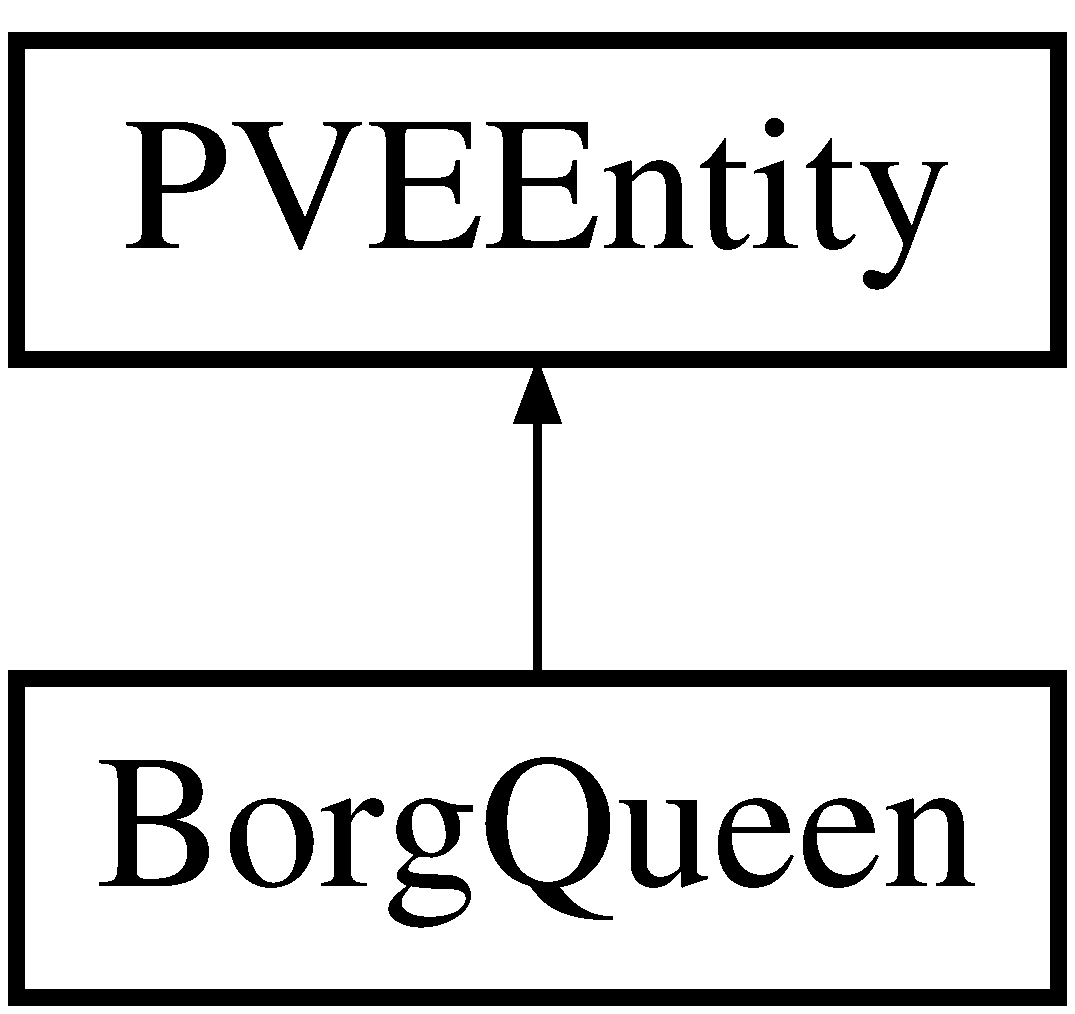
\includegraphics[height=2cm]{d6/d8d/classBorgQueen}
\end{center}
\end{figure}
\subsection*{Public Member Functions}
\begin{DoxyCompactItemize}
\item 
\hyperlink{classBorgQueen_a76607d47c521568462adcc3c3b65cbce}{BorgQueen} ()
\item 
\hyperlink{classBorgQueen_a5e2d0c2a5b5c3b00088776e2272c17f0}{$\sim$BorgQueen} ()
\item 
string \hyperlink{classBorgQueen_a51bd430d9b7b50605622d489bae898cb}{getName} ()
\item 
int \hyperlink{classBorgQueen_aa36f69293ff2c3cb5df255fee9b2d9e8}{getShieldStrenght} ()
\item 
int \hyperlink{classBorgQueen_ab7c7d1068ca9e031ab4c742d44150784}{getShieldRegenerativeRate} ()
\item 
int \hyperlink{classBorgQueen_a9f280ccd7ae93b4cf90a638189059b5b}{getRegenerativeAdaptivePlating} ()
\item 
bool \hyperlink{classBorgQueen_a269dea27e5cccc2cef605153bef654bd}{getHasRegenerativeAdaptivePlating} ()
\item 
int \hyperlink{classBorgQueen_a1d23b2f941324cb88de797090a40a406}{getTransPhasicTorpedos} ()
\item 
bool \hyperlink{classBorgQueen_a934f3c7e409e8e07fc716c53af7027ed}{getHasTransphasicTorpedos} ()
\item 
int \hyperlink{classBorgQueen_ac533d0fde52c0119abb63862b1c9b01e}{getChronitonTorpedos} ()
\item 
bool \hyperlink{classBorgQueen_a22291a2f8d58dbb517975f490ea6bad2}{getHasChronitonTorpedos} ()
\item 
int \hyperlink{classBorgQueen_ac4e4aff8c051083941bcb7d9c8ae4525}{getGravimetricTorpedos} ()
\item 
bool \hyperlink{classBorgQueen_ade43bf6397423dd698087c19ecd28707}{getHasGravimetricTorpedos} ()
\item 
int \hyperlink{classBorgQueen_a9f7a18df2032943b5211d6fa6b5a78d9}{getSpatialTorpedos} ()
\item 
bool \hyperlink{classBorgQueen_a45bff6005961ed11202666df5ad0ea5e}{getHasSpatialTorpedos} ()
\item 
bool \hyperlink{classBorgQueen_a66488c3adb0ae7603d97acd1cae540d5}{getHasLasers} ()
\item 
bool \hyperlink{classBorgQueen_ad443100edc3438d13c2125ada2e813b5}{getHasPhasedIonCannon} ()
\item 
bool \hyperlink{classBorgQueen_afff65fc18c7fca051258a34e44e1c56a}{getHasPulseWeapon} ()
\item 
int \hyperlink{classBorgQueen_aaceb90436d0f878f38346fcc6cfc846c}{getBorgComplement} ()
\item 
bool \hyperlink{classBorgQueen_a81cff66b42f357056b5eba4517b1651a}{getHasTractorLock} ()
\item 
bool \hyperlink{classBorgQueen_a52250f09cbd95239db7ea68174ad2c83}{getIsWreckPVE} ()
\item 
void \hyperlink{classBorgQueen_a28ca84d583ef28a844f420188a575d74}{setShieldStrenghtPVE} (int strenght)
\item 
void \hyperlink{classBorgQueen_adb0b4021391f1268f39c9ee5b9a0305b}{setShieldRegenerativeRatePVE} (int rate)
\item 
void \hyperlink{classBorgQueen_a0aa26287b343e1b26179d1ffd903c2f5}{setArmourPVE} (int armour)
\item 
void \hyperlink{classBorgQueen_a7533de67e36cdd6ed501c71f0ce1867f}{setTransPhasicTorpedosPVE} (int num)
\item 
void \hyperlink{classBorgQueen_a5fa2745710ae1da9d884066b8d248b9a}{setChronitonTorpedosPVE} (int num)
\item 
void \hyperlink{classBorgQueen_aff5f63cf6299acc846a40d6653dad809}{setGravimetricTorpedosPVE} (int num)
\item 
void \hyperlink{classBorgQueen_a702e59cd2edc9823b54e9db4c7edf174}{setSpatialTorpedosPVE} (int num)
\item 
void \hyperlink{classBorgQueen_af00311c06f2c000c32dc8f6837bfe945}{setHasTractorLockPVE} (bool has)
\item 
void \hyperlink{classBorgQueen_a9f508246423f214a0c585ee914d4fb96}{setWreckPVE} ()
\end{DoxyCompactItemize}


\subsection{Constructor \& Destructor Documentation}
\hypertarget{classBorgQueen_a76607d47c521568462adcc3c3b65cbce}{
\index{BorgQueen@{BorgQueen}!BorgQueen@{BorgQueen}}
\index{BorgQueen@{BorgQueen}!BorgQueen@{BorgQueen}}
\subsubsection[{BorgQueen}]{\setlength{\rightskip}{0pt plus 5cm}BorgQueen::BorgQueen ()}}
\label{d6/d8d/classBorgQueen_a76607d47c521568462adcc3c3b65cbce}
Constructor for pve entity sets up data embers based on preloaded variables arrays usning random index \hypertarget{classBorgQueen_a5e2d0c2a5b5c3b00088776e2272c17f0}{
\index{BorgQueen@{BorgQueen}!$\sim$BorgQueen@{$\sim$BorgQueen}}
\index{$\sim$BorgQueen@{$\sim$BorgQueen}!BorgQueen@{BorgQueen}}
\subsubsection[{$\sim$BorgQueen}]{\setlength{\rightskip}{0pt plus 5cm}BorgQueen::$\sim$BorgQueen ()}}
\label{d6/d8d/classBorgQueen_a5e2d0c2a5b5c3b00088776e2272c17f0}
Destructor for the enemy 

\subsection{Member Function Documentation}
\hypertarget{classBorgQueen_aaceb90436d0f878f38346fcc6cfc846c}{
\index{BorgQueen@{BorgQueen}!getBorgComplement@{getBorgComplement}}
\index{getBorgComplement@{getBorgComplement}!BorgQueen@{BorgQueen}}
\subsubsection[{getBorgComplement}]{\setlength{\rightskip}{0pt plus 5cm}int BorgQueen::getBorgComplement ()\hspace{0.3cm}{\ttfamily  \mbox{[}virtual\mbox{]}}}}
\label{d6/d8d/classBorgQueen_aaceb90436d0f878f38346fcc6cfc846c}
accessor for the enemies borg complement

\begin{DoxyReturn}{Returns}
int the borg complement data member 
\end{DoxyReturn}


Implements \hyperlink{classPVEEntity}{PVEEntity}.

\hypertarget{classBorgQueen_ac533d0fde52c0119abb63862b1c9b01e}{
\index{BorgQueen@{BorgQueen}!getChronitonTorpedos@{getChronitonTorpedos}}
\index{getChronitonTorpedos@{getChronitonTorpedos}!BorgQueen@{BorgQueen}}
\subsubsection[{getChronitonTorpedos}]{\setlength{\rightskip}{0pt plus 5cm}int BorgQueen::getChronitonTorpedos ()\hspace{0.3cm}{\ttfamily  \mbox{[}virtual\mbox{]}}}}
\label{d6/d8d/classBorgQueen_ac533d0fde52c0119abb63862b1c9b01e}
accessor for the enemies chroniton torps

\begin{DoxyReturn}{Returns}
int the chroniton torps data member 
\end{DoxyReturn}


Implements \hyperlink{classPVEEntity}{PVEEntity}.

\hypertarget{classBorgQueen_ac4e4aff8c051083941bcb7d9c8ae4525}{
\index{BorgQueen@{BorgQueen}!getGravimetricTorpedos@{getGravimetricTorpedos}}
\index{getGravimetricTorpedos@{getGravimetricTorpedos}!BorgQueen@{BorgQueen}}
\subsubsection[{getGravimetricTorpedos}]{\setlength{\rightskip}{0pt plus 5cm}int BorgQueen::getGravimetricTorpedos ()\hspace{0.3cm}{\ttfamily  \mbox{[}virtual\mbox{]}}}}
\label{d6/d8d/classBorgQueen_ac4e4aff8c051083941bcb7d9c8ae4525}
accessor for the enemies gravimetric torps

\begin{DoxyReturn}{Returns}
int the chroniton torps data member 
\end{DoxyReturn}


Implements \hyperlink{classPVEEntity}{PVEEntity}.

\hypertarget{classBorgQueen_a22291a2f8d58dbb517975f490ea6bad2}{
\index{BorgQueen@{BorgQueen}!getHasChronitonTorpedos@{getHasChronitonTorpedos}}
\index{getHasChronitonTorpedos@{getHasChronitonTorpedos}!BorgQueen@{BorgQueen}}
\subsubsection[{getHasChronitonTorpedos}]{\setlength{\rightskip}{0pt plus 5cm}bool BorgQueen::getHasChronitonTorpedos ()\hspace{0.3cm}{\ttfamily  \mbox{[}virtual\mbox{]}}}}
\label{d6/d8d/classBorgQueen_a22291a2f8d58dbb517975f490ea6bad2}
accessor for the enemies has chroniton torps

\begin{DoxyReturn}{Returns}
bool the has chroniton torps data member 
\end{DoxyReturn}


Implements \hyperlink{classPVEEntity}{PVEEntity}.

\hypertarget{classBorgQueen_ade43bf6397423dd698087c19ecd28707}{
\index{BorgQueen@{BorgQueen}!getHasGravimetricTorpedos@{getHasGravimetricTorpedos}}
\index{getHasGravimetricTorpedos@{getHasGravimetricTorpedos}!BorgQueen@{BorgQueen}}
\subsubsection[{getHasGravimetricTorpedos}]{\setlength{\rightskip}{0pt plus 5cm}bool BorgQueen::getHasGravimetricTorpedos ()\hspace{0.3cm}{\ttfamily  \mbox{[}virtual\mbox{]}}}}
\label{d6/d8d/classBorgQueen_ade43bf6397423dd698087c19ecd28707}
accessor for the enemies has gravimetric torps

\begin{DoxyReturn}{Returns}
bool the has chroniton torps data member 
\end{DoxyReturn}


Implements \hyperlink{classPVEEntity}{PVEEntity}.

\hypertarget{classBorgQueen_a66488c3adb0ae7603d97acd1cae540d5}{
\index{BorgQueen@{BorgQueen}!getHasLasers@{getHasLasers}}
\index{getHasLasers@{getHasLasers}!BorgQueen@{BorgQueen}}
\subsubsection[{getHasLasers}]{\setlength{\rightskip}{0pt plus 5cm}bool BorgQueen::getHasLasers ()\hspace{0.3cm}{\ttfamily  \mbox{[}virtual\mbox{]}}}}
\label{d6/d8d/classBorgQueen_a66488c3adb0ae7603d97acd1cae540d5}
accessor for the enemies has lasers

\begin{DoxyReturn}{Returns}
bool the has lasers data member 
\end{DoxyReturn}


Implements \hyperlink{classPVEEntity}{PVEEntity}.

\hypertarget{classBorgQueen_ad443100edc3438d13c2125ada2e813b5}{
\index{BorgQueen@{BorgQueen}!getHasPhasedIonCannon@{getHasPhasedIonCannon}}
\index{getHasPhasedIonCannon@{getHasPhasedIonCannon}!BorgQueen@{BorgQueen}}
\subsubsection[{getHasPhasedIonCannon}]{\setlength{\rightskip}{0pt plus 5cm}bool BorgQueen::getHasPhasedIonCannon ()\hspace{0.3cm}{\ttfamily  \mbox{[}virtual\mbox{]}}}}
\label{d6/d8d/classBorgQueen_ad443100edc3438d13c2125ada2e813b5}
accessor for the enemies has phased ion cannon

\begin{DoxyReturn}{Returns}
bool the has phased ion cannon data member 
\end{DoxyReturn}


Implements \hyperlink{classPVEEntity}{PVEEntity}.

\hypertarget{classBorgQueen_afff65fc18c7fca051258a34e44e1c56a}{
\index{BorgQueen@{BorgQueen}!getHasPulseWeapon@{getHasPulseWeapon}}
\index{getHasPulseWeapon@{getHasPulseWeapon}!BorgQueen@{BorgQueen}}
\subsubsection[{getHasPulseWeapon}]{\setlength{\rightskip}{0pt plus 5cm}bool BorgQueen::getHasPulseWeapon ()\hspace{0.3cm}{\ttfamily  \mbox{[}virtual\mbox{]}}}}
\label{d6/d8d/classBorgQueen_afff65fc18c7fca051258a34e44e1c56a}
accessor for the enemies has pulse weapons

\begin{DoxyReturn}{Returns}
bool the has pulse weapons data member 
\end{DoxyReturn}


Implements \hyperlink{classPVEEntity}{PVEEntity}.

\hypertarget{classBorgQueen_a269dea27e5cccc2cef605153bef654bd}{
\index{BorgQueen@{BorgQueen}!getHasRegenerativeAdaptivePlating@{getHasRegenerativeAdaptivePlating}}
\index{getHasRegenerativeAdaptivePlating@{getHasRegenerativeAdaptivePlating}!BorgQueen@{BorgQueen}}
\subsubsection[{getHasRegenerativeAdaptivePlating}]{\setlength{\rightskip}{0pt plus 5cm}bool BorgQueen::getHasRegenerativeAdaptivePlating ()\hspace{0.3cm}{\ttfamily  \mbox{[}virtual\mbox{]}}}}
\label{d6/d8d/classBorgQueen_a269dea27e5cccc2cef605153bef654bd}
accessor for the enemies has regenerative adaptive plating

\begin{DoxyReturn}{Returns}
bool the has regenerative adaptive plating data member 
\end{DoxyReturn}


Implements \hyperlink{classPVEEntity}{PVEEntity}.

\hypertarget{classBorgQueen_a45bff6005961ed11202666df5ad0ea5e}{
\index{BorgQueen@{BorgQueen}!getHasSpatialTorpedos@{getHasSpatialTorpedos}}
\index{getHasSpatialTorpedos@{getHasSpatialTorpedos}!BorgQueen@{BorgQueen}}
\subsubsection[{getHasSpatialTorpedos}]{\setlength{\rightskip}{0pt plus 5cm}bool BorgQueen::getHasSpatialTorpedos ()\hspace{0.3cm}{\ttfamily  \mbox{[}virtual\mbox{]}}}}
\label{d6/d8d/classBorgQueen_a45bff6005961ed11202666df5ad0ea5e}
accessor for the enemies has spatial torps

\begin{DoxyReturn}{Returns}
bool the has spatial torps data member 
\end{DoxyReturn}


Implements \hyperlink{classPVEEntity}{PVEEntity}.

\hypertarget{classBorgQueen_a81cff66b42f357056b5eba4517b1651a}{
\index{BorgQueen@{BorgQueen}!getHasTractorLock@{getHasTractorLock}}
\index{getHasTractorLock@{getHasTractorLock}!BorgQueen@{BorgQueen}}
\subsubsection[{getHasTractorLock}]{\setlength{\rightskip}{0pt plus 5cm}bool BorgQueen::getHasTractorLock ()\hspace{0.3cm}{\ttfamily  \mbox{[}virtual\mbox{]}}}}
\label{d6/d8d/classBorgQueen_a81cff66b42f357056b5eba4517b1651a}
accessor for the enemies tractor lock

\begin{DoxyReturn}{Returns}
bool the tractor lock data member 
\end{DoxyReturn}


Implements \hyperlink{classPVEEntity}{PVEEntity}.

\hypertarget{classBorgQueen_a934f3c7e409e8e07fc716c53af7027ed}{
\index{BorgQueen@{BorgQueen}!getHasTransphasicTorpedos@{getHasTransphasicTorpedos}}
\index{getHasTransphasicTorpedos@{getHasTransphasicTorpedos}!BorgQueen@{BorgQueen}}
\subsubsection[{getHasTransphasicTorpedos}]{\setlength{\rightskip}{0pt plus 5cm}bool BorgQueen::getHasTransphasicTorpedos ()\hspace{0.3cm}{\ttfamily  \mbox{[}virtual\mbox{]}}}}
\label{d6/d8d/classBorgQueen_a934f3c7e409e8e07fc716c53af7027ed}
accessor for the enemies has transphasic torps

\begin{DoxyReturn}{Returns}
bool the has transphasic torps data member 
\end{DoxyReturn}


Implements \hyperlink{classPVEEntity}{PVEEntity}.

\hypertarget{classBorgQueen_a52250f09cbd95239db7ea68174ad2c83}{
\index{BorgQueen@{BorgQueen}!getIsWreckPVE@{getIsWreckPVE}}
\index{getIsWreckPVE@{getIsWreckPVE}!BorgQueen@{BorgQueen}}
\subsubsection[{getIsWreckPVE}]{\setlength{\rightskip}{0pt plus 5cm}bool BorgQueen::getIsWreckPVE ()\hspace{0.3cm}{\ttfamily  \mbox{[}virtual\mbox{]}}}}
\label{d6/d8d/classBorgQueen_a52250f09cbd95239db7ea68174ad2c83}
accessor for the enemies wreck status

\begin{DoxyReturn}{Returns}
bool the wreck status data member 
\end{DoxyReturn}


Implements \hyperlink{classPVEEntity}{PVEEntity}.

\hypertarget{classBorgQueen_a51bd430d9b7b50605622d489bae898cb}{
\index{BorgQueen@{BorgQueen}!getName@{getName}}
\index{getName@{getName}!BorgQueen@{BorgQueen}}
\subsubsection[{getName}]{\setlength{\rightskip}{0pt plus 5cm}string BorgQueen::getName ()\hspace{0.3cm}{\ttfamily  \mbox{[}virtual\mbox{]}}}}
\label{d6/d8d/classBorgQueen_a51bd430d9b7b50605622d489bae898cb}
accessor for the enemies name

\begin{DoxyReturn}{Returns}
string the enemies name 
\end{DoxyReturn}


Implements \hyperlink{classPVEEntity}{PVEEntity}.

\hypertarget{classBorgQueen_a9f280ccd7ae93b4cf90a638189059b5b}{
\index{BorgQueen@{BorgQueen}!getRegenerativeAdaptivePlating@{getRegenerativeAdaptivePlating}}
\index{getRegenerativeAdaptivePlating@{getRegenerativeAdaptivePlating}!BorgQueen@{BorgQueen}}
\subsubsection[{getRegenerativeAdaptivePlating}]{\setlength{\rightskip}{0pt plus 5cm}int BorgQueen::getRegenerativeAdaptivePlating ()\hspace{0.3cm}{\ttfamily  \mbox{[}virtual\mbox{]}}}}
\label{d6/d8d/classBorgQueen_a9f280ccd7ae93b4cf90a638189059b5b}
accessor for the enemies regenerative adaptive plating

\begin{DoxyReturn}{Returns}
int the regenerative adaptive plating data member 
\end{DoxyReturn}


Implements \hyperlink{classPVEEntity}{PVEEntity}.

\hypertarget{classBorgQueen_ab7c7d1068ca9e031ab4c742d44150784}{
\index{BorgQueen@{BorgQueen}!getShieldRegenerativeRate@{getShieldRegenerativeRate}}
\index{getShieldRegenerativeRate@{getShieldRegenerativeRate}!BorgQueen@{BorgQueen}}
\subsubsection[{getShieldRegenerativeRate}]{\setlength{\rightskip}{0pt plus 5cm}int BorgQueen::getShieldRegenerativeRate ()\hspace{0.3cm}{\ttfamily  \mbox{[}virtual\mbox{]}}}}
\label{d6/d8d/classBorgQueen_ab7c7d1068ca9e031ab4c742d44150784}
accessor for the enemies shield regenerative rate

\begin{DoxyReturn}{Returns}
int the shield regenerative rate data member 
\end{DoxyReturn}


Implements \hyperlink{classPVEEntity}{PVEEntity}.

\hypertarget{classBorgQueen_aa36f69293ff2c3cb5df255fee9b2d9e8}{
\index{BorgQueen@{BorgQueen}!getShieldStrenght@{getShieldStrenght}}
\index{getShieldStrenght@{getShieldStrenght}!BorgQueen@{BorgQueen}}
\subsubsection[{getShieldStrenght}]{\setlength{\rightskip}{0pt plus 5cm}int BorgQueen::getShieldStrenght ()\hspace{0.3cm}{\ttfamily  \mbox{[}virtual\mbox{]}}}}
\label{d6/d8d/classBorgQueen_aa36f69293ff2c3cb5df255fee9b2d9e8}
accessor for the enemies shield strength

\begin{DoxyReturn}{Returns}
int the shield strength data member 
\end{DoxyReturn}


Implements \hyperlink{classPVEEntity}{PVEEntity}.

\hypertarget{classBorgQueen_a9f7a18df2032943b5211d6fa6b5a78d9}{
\index{BorgQueen@{BorgQueen}!getSpatialTorpedos@{getSpatialTorpedos}}
\index{getSpatialTorpedos@{getSpatialTorpedos}!BorgQueen@{BorgQueen}}
\subsubsection[{getSpatialTorpedos}]{\setlength{\rightskip}{0pt plus 5cm}int BorgQueen::getSpatialTorpedos ()\hspace{0.3cm}{\ttfamily  \mbox{[}virtual\mbox{]}}}}
\label{d6/d8d/classBorgQueen_a9f7a18df2032943b5211d6fa6b5a78d9}
accessor for the enemies spatial torps

\begin{DoxyReturn}{Returns}
int the spatial torps data member 
\end{DoxyReturn}


Implements \hyperlink{classPVEEntity}{PVEEntity}.

\hypertarget{classBorgQueen_a1d23b2f941324cb88de797090a40a406}{
\index{BorgQueen@{BorgQueen}!getTransPhasicTorpedos@{getTransPhasicTorpedos}}
\index{getTransPhasicTorpedos@{getTransPhasicTorpedos}!BorgQueen@{BorgQueen}}
\subsubsection[{getTransPhasicTorpedos}]{\setlength{\rightskip}{0pt plus 5cm}int BorgQueen::getTransPhasicTorpedos ()\hspace{0.3cm}{\ttfamily  \mbox{[}virtual\mbox{]}}}}
\label{d6/d8d/classBorgQueen_a1d23b2f941324cb88de797090a40a406}
accessor for the enemies has regenerative adaptive plating

\begin{DoxyReturn}{Returns}
bool the has regenerative adaptive plating data member 
\end{DoxyReturn}


Implements \hyperlink{classPVEEntity}{PVEEntity}.

\hypertarget{classBorgQueen_a0aa26287b343e1b26179d1ffd903c2f5}{
\index{BorgQueen@{BorgQueen}!setArmourPVE@{setArmourPVE}}
\index{setArmourPVE@{setArmourPVE}!BorgQueen@{BorgQueen}}
\subsubsection[{setArmourPVE}]{\setlength{\rightskip}{0pt plus 5cm}void BorgQueen::setArmourPVE (int {\em armour})\hspace{0.3cm}{\ttfamily  \mbox{[}virtual\mbox{]}}}}
\label{d6/d8d/classBorgQueen_a0aa26287b343e1b26179d1ffd903c2f5}
mutator for the enemies armour


\begin{DoxyParams}{Parameters}
\item[{\em armour}]the value to set the data member\end{DoxyParams}
\begin{DoxyReturn}{Returns}
void 
\end{DoxyReturn}


Implements \hyperlink{classPVEEntity}{PVEEntity}.

\hypertarget{classBorgQueen_a5fa2745710ae1da9d884066b8d248b9a}{
\index{BorgQueen@{BorgQueen}!setChronitonTorpedosPVE@{setChronitonTorpedosPVE}}
\index{setChronitonTorpedosPVE@{setChronitonTorpedosPVE}!BorgQueen@{BorgQueen}}
\subsubsection[{setChronitonTorpedosPVE}]{\setlength{\rightskip}{0pt plus 5cm}void BorgQueen::setChronitonTorpedosPVE (int {\em num})\hspace{0.3cm}{\ttfamily  \mbox{[}virtual\mbox{]}}}}
\label{d6/d8d/classBorgQueen_a5fa2745710ae1da9d884066b8d248b9a}
mutator for the enemies chroniton torps


\begin{DoxyParams}{Parameters}
\item[{\em num}]the value to set the data member\end{DoxyParams}
\begin{DoxyReturn}{Returns}
void 
\end{DoxyReturn}


Implements \hyperlink{classPVEEntity}{PVEEntity}.

\hypertarget{classBorgQueen_aff5f63cf6299acc846a40d6653dad809}{
\index{BorgQueen@{BorgQueen}!setGravimetricTorpedosPVE@{setGravimetricTorpedosPVE}}
\index{setGravimetricTorpedosPVE@{setGravimetricTorpedosPVE}!BorgQueen@{BorgQueen}}
\subsubsection[{setGravimetricTorpedosPVE}]{\setlength{\rightskip}{0pt plus 5cm}void BorgQueen::setGravimetricTorpedosPVE (int {\em num})\hspace{0.3cm}{\ttfamily  \mbox{[}virtual\mbox{]}}}}
\label{d6/d8d/classBorgQueen_aff5f63cf6299acc846a40d6653dad809}
mutator for the enemies gravimetric torps


\begin{DoxyParams}{Parameters}
\item[{\em num}]the value to set the data member\end{DoxyParams}
\begin{DoxyReturn}{Returns}
void 
\end{DoxyReturn}


Implements \hyperlink{classPVEEntity}{PVEEntity}.

\hypertarget{classBorgQueen_af00311c06f2c000c32dc8f6837bfe945}{
\index{BorgQueen@{BorgQueen}!setHasTractorLockPVE@{setHasTractorLockPVE}}
\index{setHasTractorLockPVE@{setHasTractorLockPVE}!BorgQueen@{BorgQueen}}
\subsubsection[{setHasTractorLockPVE}]{\setlength{\rightskip}{0pt plus 5cm}void BorgQueen::setHasTractorLockPVE (bool {\em has})\hspace{0.3cm}{\ttfamily  \mbox{[}virtual\mbox{]}}}}
\label{d6/d8d/classBorgQueen_af00311c06f2c000c32dc8f6837bfe945}
mutator for the enemies tractor beam


\begin{DoxyParams}{Parameters}
\item[{\em has}]the bool value to set the data member\end{DoxyParams}
\begin{DoxyReturn}{Returns}
void 
\end{DoxyReturn}


Implements \hyperlink{classPVEEntity}{PVEEntity}.

\hypertarget{classBorgQueen_adb0b4021391f1268f39c9ee5b9a0305b}{
\index{BorgQueen@{BorgQueen}!setShieldRegenerativeRatePVE@{setShieldRegenerativeRatePVE}}
\index{setShieldRegenerativeRatePVE@{setShieldRegenerativeRatePVE}!BorgQueen@{BorgQueen}}
\subsubsection[{setShieldRegenerativeRatePVE}]{\setlength{\rightskip}{0pt plus 5cm}void BorgQueen::setShieldRegenerativeRatePVE (int {\em rate})\hspace{0.3cm}{\ttfamily  \mbox{[}virtual\mbox{]}}}}
\label{d6/d8d/classBorgQueen_adb0b4021391f1268f39c9ee5b9a0305b}
mutator for the enemies regenerative rate


\begin{DoxyParams}{Parameters}
\item[{\em rate}]the value to set the data member\end{DoxyParams}
\begin{DoxyReturn}{Returns}
void 
\end{DoxyReturn}


Implements \hyperlink{classPVEEntity}{PVEEntity}.

\hypertarget{classBorgQueen_a28ca84d583ef28a844f420188a575d74}{
\index{BorgQueen@{BorgQueen}!setShieldStrenghtPVE@{setShieldStrenghtPVE}}
\index{setShieldStrenghtPVE@{setShieldStrenghtPVE}!BorgQueen@{BorgQueen}}
\subsubsection[{setShieldStrenghtPVE}]{\setlength{\rightskip}{0pt plus 5cm}void BorgQueen::setShieldStrenghtPVE (int {\em strenght})\hspace{0.3cm}{\ttfamily  \mbox{[}virtual\mbox{]}}}}
\label{d6/d8d/classBorgQueen_a28ca84d583ef28a844f420188a575d74}
mutator for the enemies shield strength


\begin{DoxyParams}{Parameters}
\item[{\em strenght}]the value to set the data member\end{DoxyParams}
\begin{DoxyReturn}{Returns}
void 
\end{DoxyReturn}


Implements \hyperlink{classPVEEntity}{PVEEntity}.

\hypertarget{classBorgQueen_a702e59cd2edc9823b54e9db4c7edf174}{
\index{BorgQueen@{BorgQueen}!setSpatialTorpedosPVE@{setSpatialTorpedosPVE}}
\index{setSpatialTorpedosPVE@{setSpatialTorpedosPVE}!BorgQueen@{BorgQueen}}
\subsubsection[{setSpatialTorpedosPVE}]{\setlength{\rightskip}{0pt plus 5cm}void BorgQueen::setSpatialTorpedosPVE (int {\em num})\hspace{0.3cm}{\ttfamily  \mbox{[}virtual\mbox{]}}}}
\label{d6/d8d/classBorgQueen_a702e59cd2edc9823b54e9db4c7edf174}
mutator for the enemies spatial torps


\begin{DoxyParams}{Parameters}
\item[{\em num}]the value to set the data member\end{DoxyParams}
\begin{DoxyReturn}{Returns}
void 
\end{DoxyReturn}


Implements \hyperlink{classPVEEntity}{PVEEntity}.

\hypertarget{classBorgQueen_a7533de67e36cdd6ed501c71f0ce1867f}{
\index{BorgQueen@{BorgQueen}!setTransPhasicTorpedosPVE@{setTransPhasicTorpedosPVE}}
\index{setTransPhasicTorpedosPVE@{setTransPhasicTorpedosPVE}!BorgQueen@{BorgQueen}}
\subsubsection[{setTransPhasicTorpedosPVE}]{\setlength{\rightskip}{0pt plus 5cm}void BorgQueen::setTransPhasicTorpedosPVE (int {\em num})\hspace{0.3cm}{\ttfamily  \mbox{[}virtual\mbox{]}}}}
\label{d6/d8d/classBorgQueen_a7533de67e36cdd6ed501c71f0ce1867f}
mutator for the enemies trans phasic torps


\begin{DoxyParams}{Parameters}
\item[{\em num}]the value to set the data member\end{DoxyParams}
\begin{DoxyReturn}{Returns}
void 
\end{DoxyReturn}


Implements \hyperlink{classPVEEntity}{PVEEntity}.

\hypertarget{classBorgQueen_a9f508246423f214a0c585ee914d4fb96}{
\index{BorgQueen@{BorgQueen}!setWreckPVE@{setWreckPVE}}
\index{setWreckPVE@{setWreckPVE}!BorgQueen@{BorgQueen}}
\subsubsection[{setWreckPVE}]{\setlength{\rightskip}{0pt plus 5cm}void BorgQueen::setWreckPVE ()\hspace{0.3cm}{\ttfamily  \mbox{[}virtual\mbox{]}}}}
\label{d6/d8d/classBorgQueen_a9f508246423f214a0c585ee914d4fb96}
mutator for the enemies wreck state

\begin{DoxyReturn}{Returns}
void 
\end{DoxyReturn}


Implements \hyperlink{classPVEEntity}{PVEEntity}.



The documentation for this class was generated from the following files:\begin{DoxyCompactItemize}
\item 
source/header/BorgQueen.h\item 
source/source/BorgQueen.cpp\end{DoxyCompactItemize}

\hypertarget{classBorgRogue}{
\section{BorgRogue Class Reference}
\label{db/d4f/classBorgRogue}\index{BorgRogue@{BorgRogue}}
}
Inheritance diagram for BorgRogue:\begin{figure}[H]
\begin{center}
\leavevmode
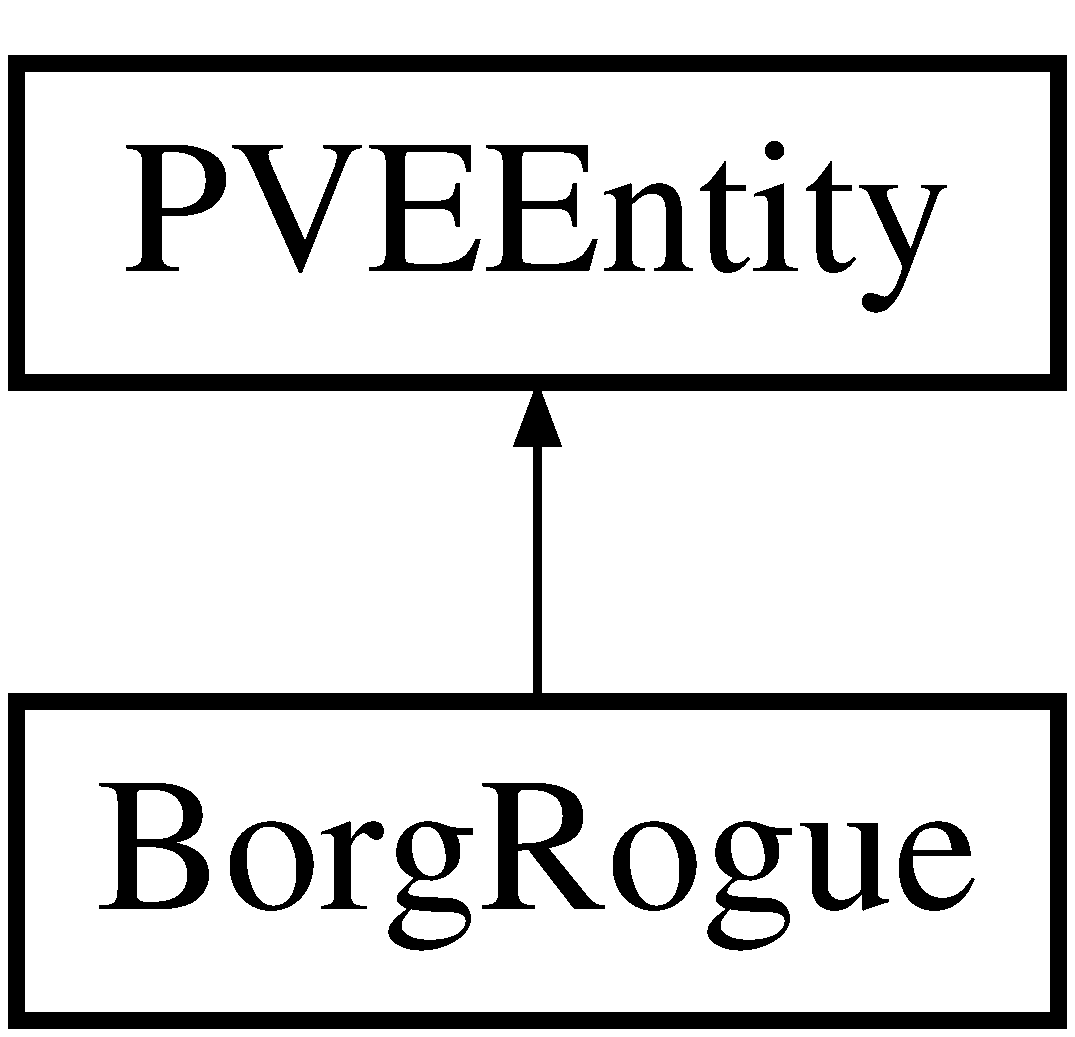
\includegraphics[height=2cm]{db/d4f/classBorgRogue}
\end{center}
\end{figure}
\subsection*{Public Member Functions}
\begin{DoxyCompactItemize}
\item 
\hyperlink{classBorgRogue_ac7a4f4b617206d1b2ef3489a533f69e9}{BorgRogue} ()
\item 
\hyperlink{classBorgRogue_a1afdc1a65a85e59f0e598a4877f173b7}{$\sim$BorgRogue} ()
\item 
string \hyperlink{classBorgRogue_ac4b4cf44886438d6e4cd6933ac46ae0e}{getName} ()
\item 
int \hyperlink{classBorgRogue_a8d64c0f319f734e69aa9592cbaf29892}{getShieldStrenght} ()
\item 
int \hyperlink{classBorgRogue_a055c08424838cd6defd5d264b9d55532}{getShieldRegenerativeRate} ()
\item 
int \hyperlink{classBorgRogue_ac5d9f8c62b43fefdc61fe672a8510fa0}{getRegenerativeAdaptivePlating} ()
\item 
bool \hyperlink{classBorgRogue_aff3dbb33470200cc97860ca2d4b22ca5}{getHasRegenerativeAdaptivePlating} ()
\item 
int \hyperlink{classBorgRogue_ab8d59b4fb9983b55896a0790e701ff7a}{getTransPhasicTorpedos} ()
\item 
bool \hyperlink{classBorgRogue_a2b62489036e3bd2e1ce51fbb06f90ec2}{getHasTransphasicTorpedos} ()
\item 
int \hyperlink{classBorgRogue_a6403ee1ec00f94a9607a35b77b539e78}{getChronitonTorpedos} ()
\item 
bool \hyperlink{classBorgRogue_a8e4728091fa86cc8cf1122975f4fd9e4}{getHasChronitonTorpedos} ()
\item 
int \hyperlink{classBorgRogue_af1d6b12ee69cdc85a2417c1b25d36f19}{getGravimetricTorpedos} ()
\item 
bool \hyperlink{classBorgRogue_a1f4fd1ce4d664b532c7095513f530241}{getHasGravimetricTorpedos} ()
\item 
int \hyperlink{classBorgRogue_ad79dc4b3ce9c83724fc250cb918bcb8f}{getSpatialTorpedos} ()
\item 
bool \hyperlink{classBorgRogue_ae3dc5dcd0f872f8960799795882231de}{getHasSpatialTorpedos} ()
\item 
bool \hyperlink{classBorgRogue_a9a32c764b84654af68bfcc3fc934460c}{getHasLasers} ()
\item 
bool \hyperlink{classBorgRogue_af2c0c7885c76c080c2e255069672c13b}{getHasPhasedIonCannon} ()
\item 
bool \hyperlink{classBorgRogue_acfd7c55d67ff89410eed4270c88f0e2f}{getHasPulseWeapon} ()
\item 
int \hyperlink{classBorgRogue_ab48a76b7a43d96a9b7f63f5b7cdc01d7}{getBorgComplement} ()
\item 
bool \hyperlink{classBorgRogue_aece2200d14e0f1e3056ea52290a39f27}{getHasTractorLock} ()
\item 
bool \hyperlink{classBorgRogue_ac51cbf466e2db63dc9dd895cea4e1977}{getIsWreckPVE} ()
\item 
void \hyperlink{classBorgRogue_a99ce619718648684b12ffdbaa7fd983f}{setShieldStrenghtPVE} (int strenght)
\item 
void \hyperlink{classBorgRogue_afaa9f67e6e5536b0aa63ce8120c0247f}{setShieldRegenerativeRatePVE} (int rate)
\item 
void \hyperlink{classBorgRogue_af34a5a35c56e8a4758fa69e6937405d1}{setArmourPVE} (int armour)
\item 
void \hyperlink{classBorgRogue_aa758dd218dae6a330f53ec54e904831b}{setTransPhasicTorpedosPVE} (int num)
\item 
void \hyperlink{classBorgRogue_a1cf5168c6189366bd40bae7ec414b17f}{setChronitonTorpedosPVE} (int num)
\item 
void \hyperlink{classBorgRogue_a73ff2f1ab55d607fa9a39cfda5c22a8d}{setGravimetricTorpedosPVE} (int num)
\item 
void \hyperlink{classBorgRogue_ad983f34e403f754d256527f784465ba5}{setSpatialTorpedosPVE} (int num)
\item 
void \hyperlink{classBorgRogue_a81779a2a3027c82452c17fd0503f7d2c}{setHasTractorLockPVE} (bool has)
\item 
void \hyperlink{classBorgRogue_a534229bde2f85076dc13d0b5a7b7afb1}{setWreckPVE} ()
\end{DoxyCompactItemize}


\subsection{Constructor \& Destructor Documentation}
\hypertarget{classBorgRogue_ac7a4f4b617206d1b2ef3489a533f69e9}{
\index{BorgRogue@{BorgRogue}!BorgRogue@{BorgRogue}}
\index{BorgRogue@{BorgRogue}!BorgRogue@{BorgRogue}}
\subsubsection[{BorgRogue}]{\setlength{\rightskip}{0pt plus 5cm}BorgRogue::BorgRogue ()}}
\label{db/d4f/classBorgRogue_ac7a4f4b617206d1b2ef3489a533f69e9}
Constructor for pve entity sets up data embers based on preloaded variables arrays usning random index \hypertarget{classBorgRogue_a1afdc1a65a85e59f0e598a4877f173b7}{
\index{BorgRogue@{BorgRogue}!$\sim$BorgRogue@{$\sim$BorgRogue}}
\index{$\sim$BorgRogue@{$\sim$BorgRogue}!BorgRogue@{BorgRogue}}
\subsubsection[{$\sim$BorgRogue}]{\setlength{\rightskip}{0pt plus 5cm}BorgRogue::$\sim$BorgRogue ()}}
\label{db/d4f/classBorgRogue_a1afdc1a65a85e59f0e598a4877f173b7}
Destructor for the enemy 

\subsection{Member Function Documentation}
\hypertarget{classBorgRogue_ab48a76b7a43d96a9b7f63f5b7cdc01d7}{
\index{BorgRogue@{BorgRogue}!getBorgComplement@{getBorgComplement}}
\index{getBorgComplement@{getBorgComplement}!BorgRogue@{BorgRogue}}
\subsubsection[{getBorgComplement}]{\setlength{\rightskip}{0pt plus 5cm}int BorgRogue::getBorgComplement ()\hspace{0.3cm}{\ttfamily  \mbox{[}virtual\mbox{]}}}}
\label{db/d4f/classBorgRogue_ab48a76b7a43d96a9b7f63f5b7cdc01d7}
accessor for the enemies borg complement

\begin{DoxyReturn}{Returns}
int the borg complement data member 
\end{DoxyReturn}


Implements \hyperlink{classPVEEntity}{PVEEntity}.

\hypertarget{classBorgRogue_a6403ee1ec00f94a9607a35b77b539e78}{
\index{BorgRogue@{BorgRogue}!getChronitonTorpedos@{getChronitonTorpedos}}
\index{getChronitonTorpedos@{getChronitonTorpedos}!BorgRogue@{BorgRogue}}
\subsubsection[{getChronitonTorpedos}]{\setlength{\rightskip}{0pt plus 5cm}int BorgRogue::getChronitonTorpedos ()\hspace{0.3cm}{\ttfamily  \mbox{[}virtual\mbox{]}}}}
\label{db/d4f/classBorgRogue_a6403ee1ec00f94a9607a35b77b539e78}
accessor for the enemies chroniton torps

\begin{DoxyReturn}{Returns}
int the chroniton torps data member 
\end{DoxyReturn}


Implements \hyperlink{classPVEEntity}{PVEEntity}.

\hypertarget{classBorgRogue_af1d6b12ee69cdc85a2417c1b25d36f19}{
\index{BorgRogue@{BorgRogue}!getGravimetricTorpedos@{getGravimetricTorpedos}}
\index{getGravimetricTorpedos@{getGravimetricTorpedos}!BorgRogue@{BorgRogue}}
\subsubsection[{getGravimetricTorpedos}]{\setlength{\rightskip}{0pt plus 5cm}int BorgRogue::getGravimetricTorpedos ()\hspace{0.3cm}{\ttfamily  \mbox{[}virtual\mbox{]}}}}
\label{db/d4f/classBorgRogue_af1d6b12ee69cdc85a2417c1b25d36f19}
accessor for the enemies gravimetric torps

\begin{DoxyReturn}{Returns}
int the chroniton torps data member 
\end{DoxyReturn}


Implements \hyperlink{classPVEEntity}{PVEEntity}.

\hypertarget{classBorgRogue_a8e4728091fa86cc8cf1122975f4fd9e4}{
\index{BorgRogue@{BorgRogue}!getHasChronitonTorpedos@{getHasChronitonTorpedos}}
\index{getHasChronitonTorpedos@{getHasChronitonTorpedos}!BorgRogue@{BorgRogue}}
\subsubsection[{getHasChronitonTorpedos}]{\setlength{\rightskip}{0pt plus 5cm}bool BorgRogue::getHasChronitonTorpedos ()\hspace{0.3cm}{\ttfamily  \mbox{[}virtual\mbox{]}}}}
\label{db/d4f/classBorgRogue_a8e4728091fa86cc8cf1122975f4fd9e4}
accessor for the enemies has chroniton torps

\begin{DoxyReturn}{Returns}
bool the has chroniton torps data member 
\end{DoxyReturn}


Implements \hyperlink{classPVEEntity}{PVEEntity}.

\hypertarget{classBorgRogue_a1f4fd1ce4d664b532c7095513f530241}{
\index{BorgRogue@{BorgRogue}!getHasGravimetricTorpedos@{getHasGravimetricTorpedos}}
\index{getHasGravimetricTorpedos@{getHasGravimetricTorpedos}!BorgRogue@{BorgRogue}}
\subsubsection[{getHasGravimetricTorpedos}]{\setlength{\rightskip}{0pt plus 5cm}bool BorgRogue::getHasGravimetricTorpedos ()\hspace{0.3cm}{\ttfamily  \mbox{[}virtual\mbox{]}}}}
\label{db/d4f/classBorgRogue_a1f4fd1ce4d664b532c7095513f530241}
accessor for the enemies has gravimetric torps

\begin{DoxyReturn}{Returns}
bool the has chroniton torps data member 
\end{DoxyReturn}


Implements \hyperlink{classPVEEntity}{PVEEntity}.

\hypertarget{classBorgRogue_a9a32c764b84654af68bfcc3fc934460c}{
\index{BorgRogue@{BorgRogue}!getHasLasers@{getHasLasers}}
\index{getHasLasers@{getHasLasers}!BorgRogue@{BorgRogue}}
\subsubsection[{getHasLasers}]{\setlength{\rightskip}{0pt plus 5cm}bool BorgRogue::getHasLasers ()\hspace{0.3cm}{\ttfamily  \mbox{[}virtual\mbox{]}}}}
\label{db/d4f/classBorgRogue_a9a32c764b84654af68bfcc3fc934460c}
accessor for the enemies has lasers

\begin{DoxyReturn}{Returns}
bool the has lasers data member 
\end{DoxyReturn}


Implements \hyperlink{classPVEEntity}{PVEEntity}.

\hypertarget{classBorgRogue_af2c0c7885c76c080c2e255069672c13b}{
\index{BorgRogue@{BorgRogue}!getHasPhasedIonCannon@{getHasPhasedIonCannon}}
\index{getHasPhasedIonCannon@{getHasPhasedIonCannon}!BorgRogue@{BorgRogue}}
\subsubsection[{getHasPhasedIonCannon}]{\setlength{\rightskip}{0pt plus 5cm}bool BorgRogue::getHasPhasedIonCannon ()\hspace{0.3cm}{\ttfamily  \mbox{[}virtual\mbox{]}}}}
\label{db/d4f/classBorgRogue_af2c0c7885c76c080c2e255069672c13b}
accessor for the enemies has phased ion cannon

\begin{DoxyReturn}{Returns}
bool the has phased ion cannon data member 
\end{DoxyReturn}


Implements \hyperlink{classPVEEntity}{PVEEntity}.

\hypertarget{classBorgRogue_acfd7c55d67ff89410eed4270c88f0e2f}{
\index{BorgRogue@{BorgRogue}!getHasPulseWeapon@{getHasPulseWeapon}}
\index{getHasPulseWeapon@{getHasPulseWeapon}!BorgRogue@{BorgRogue}}
\subsubsection[{getHasPulseWeapon}]{\setlength{\rightskip}{0pt plus 5cm}bool BorgRogue::getHasPulseWeapon ()\hspace{0.3cm}{\ttfamily  \mbox{[}virtual\mbox{]}}}}
\label{db/d4f/classBorgRogue_acfd7c55d67ff89410eed4270c88f0e2f}
accessor for the enemies has pulse weapons

\begin{DoxyReturn}{Returns}
bool the has pulse weapons data member 
\end{DoxyReturn}


Implements \hyperlink{classPVEEntity}{PVEEntity}.

\hypertarget{classBorgRogue_aff3dbb33470200cc97860ca2d4b22ca5}{
\index{BorgRogue@{BorgRogue}!getHasRegenerativeAdaptivePlating@{getHasRegenerativeAdaptivePlating}}
\index{getHasRegenerativeAdaptivePlating@{getHasRegenerativeAdaptivePlating}!BorgRogue@{BorgRogue}}
\subsubsection[{getHasRegenerativeAdaptivePlating}]{\setlength{\rightskip}{0pt plus 5cm}bool BorgRogue::getHasRegenerativeAdaptivePlating ()\hspace{0.3cm}{\ttfamily  \mbox{[}virtual\mbox{]}}}}
\label{db/d4f/classBorgRogue_aff3dbb33470200cc97860ca2d4b22ca5}
accessor for the enemies has regenerative adaptive plating

\begin{DoxyReturn}{Returns}
bool the has regenerative adaptive plating data member 
\end{DoxyReturn}


Implements \hyperlink{classPVEEntity}{PVEEntity}.

\hypertarget{classBorgRogue_ae3dc5dcd0f872f8960799795882231de}{
\index{BorgRogue@{BorgRogue}!getHasSpatialTorpedos@{getHasSpatialTorpedos}}
\index{getHasSpatialTorpedos@{getHasSpatialTorpedos}!BorgRogue@{BorgRogue}}
\subsubsection[{getHasSpatialTorpedos}]{\setlength{\rightskip}{0pt plus 5cm}bool BorgRogue::getHasSpatialTorpedos ()\hspace{0.3cm}{\ttfamily  \mbox{[}virtual\mbox{]}}}}
\label{db/d4f/classBorgRogue_ae3dc5dcd0f872f8960799795882231de}
accessor for the enemies has spatial torps

\begin{DoxyReturn}{Returns}
bool the has spatial torps data member 
\end{DoxyReturn}


Implements \hyperlink{classPVEEntity}{PVEEntity}.

\hypertarget{classBorgRogue_aece2200d14e0f1e3056ea52290a39f27}{
\index{BorgRogue@{BorgRogue}!getHasTractorLock@{getHasTractorLock}}
\index{getHasTractorLock@{getHasTractorLock}!BorgRogue@{BorgRogue}}
\subsubsection[{getHasTractorLock}]{\setlength{\rightskip}{0pt plus 5cm}bool BorgRogue::getHasTractorLock ()\hspace{0.3cm}{\ttfamily  \mbox{[}virtual\mbox{]}}}}
\label{db/d4f/classBorgRogue_aece2200d14e0f1e3056ea52290a39f27}
accessor for the enemies tractor lock

\begin{DoxyReturn}{Returns}
bool the tractor lock data member 
\end{DoxyReturn}


Implements \hyperlink{classPVEEntity}{PVEEntity}.

\hypertarget{classBorgRogue_a2b62489036e3bd2e1ce51fbb06f90ec2}{
\index{BorgRogue@{BorgRogue}!getHasTransphasicTorpedos@{getHasTransphasicTorpedos}}
\index{getHasTransphasicTorpedos@{getHasTransphasicTorpedos}!BorgRogue@{BorgRogue}}
\subsubsection[{getHasTransphasicTorpedos}]{\setlength{\rightskip}{0pt plus 5cm}bool BorgRogue::getHasTransphasicTorpedos ()\hspace{0.3cm}{\ttfamily  \mbox{[}virtual\mbox{]}}}}
\label{db/d4f/classBorgRogue_a2b62489036e3bd2e1ce51fbb06f90ec2}
accessor for the enemies has transphasic torps

\begin{DoxyReturn}{Returns}
bool the has transphasic torps data member 
\end{DoxyReturn}


Implements \hyperlink{classPVEEntity}{PVEEntity}.

\hypertarget{classBorgRogue_ac51cbf466e2db63dc9dd895cea4e1977}{
\index{BorgRogue@{BorgRogue}!getIsWreckPVE@{getIsWreckPVE}}
\index{getIsWreckPVE@{getIsWreckPVE}!BorgRogue@{BorgRogue}}
\subsubsection[{getIsWreckPVE}]{\setlength{\rightskip}{0pt plus 5cm}bool BorgRogue::getIsWreckPVE ()\hspace{0.3cm}{\ttfamily  \mbox{[}virtual\mbox{]}}}}
\label{db/d4f/classBorgRogue_ac51cbf466e2db63dc9dd895cea4e1977}
accessor for the enemies wreck status

\begin{DoxyReturn}{Returns}
bool the wreck status data member 
\end{DoxyReturn}


Implements \hyperlink{classPVEEntity}{PVEEntity}.

\hypertarget{classBorgRogue_ac4b4cf44886438d6e4cd6933ac46ae0e}{
\index{BorgRogue@{BorgRogue}!getName@{getName}}
\index{getName@{getName}!BorgRogue@{BorgRogue}}
\subsubsection[{getName}]{\setlength{\rightskip}{0pt plus 5cm}string BorgRogue::getName ()\hspace{0.3cm}{\ttfamily  \mbox{[}virtual\mbox{]}}}}
\label{db/d4f/classBorgRogue_ac4b4cf44886438d6e4cd6933ac46ae0e}
accessor for the enemies name

\begin{DoxyReturn}{Returns}
string the enemies name 
\end{DoxyReturn}


Implements \hyperlink{classPVEEntity}{PVEEntity}.

\hypertarget{classBorgRogue_ac5d9f8c62b43fefdc61fe672a8510fa0}{
\index{BorgRogue@{BorgRogue}!getRegenerativeAdaptivePlating@{getRegenerativeAdaptivePlating}}
\index{getRegenerativeAdaptivePlating@{getRegenerativeAdaptivePlating}!BorgRogue@{BorgRogue}}
\subsubsection[{getRegenerativeAdaptivePlating}]{\setlength{\rightskip}{0pt plus 5cm}int BorgRogue::getRegenerativeAdaptivePlating ()\hspace{0.3cm}{\ttfamily  \mbox{[}virtual\mbox{]}}}}
\label{db/d4f/classBorgRogue_ac5d9f8c62b43fefdc61fe672a8510fa0}
accessor for the enemies regenerative adaptive plating

\begin{DoxyReturn}{Returns}
int the regenerative adaptive plating data member 
\end{DoxyReturn}


Implements \hyperlink{classPVEEntity}{PVEEntity}.

\hypertarget{classBorgRogue_a055c08424838cd6defd5d264b9d55532}{
\index{BorgRogue@{BorgRogue}!getShieldRegenerativeRate@{getShieldRegenerativeRate}}
\index{getShieldRegenerativeRate@{getShieldRegenerativeRate}!BorgRogue@{BorgRogue}}
\subsubsection[{getShieldRegenerativeRate}]{\setlength{\rightskip}{0pt plus 5cm}int BorgRogue::getShieldRegenerativeRate ()\hspace{0.3cm}{\ttfamily  \mbox{[}virtual\mbox{]}}}}
\label{db/d4f/classBorgRogue_a055c08424838cd6defd5d264b9d55532}
accessor for the enemies shield regenerative rate

\begin{DoxyReturn}{Returns}
int the shield regenerative rate data member 
\end{DoxyReturn}


Implements \hyperlink{classPVEEntity}{PVEEntity}.

\hypertarget{classBorgRogue_a8d64c0f319f734e69aa9592cbaf29892}{
\index{BorgRogue@{BorgRogue}!getShieldStrenght@{getShieldStrenght}}
\index{getShieldStrenght@{getShieldStrenght}!BorgRogue@{BorgRogue}}
\subsubsection[{getShieldStrenght}]{\setlength{\rightskip}{0pt plus 5cm}int BorgRogue::getShieldStrenght ()\hspace{0.3cm}{\ttfamily  \mbox{[}virtual\mbox{]}}}}
\label{db/d4f/classBorgRogue_a8d64c0f319f734e69aa9592cbaf29892}
accessor for the enemies shield strength

\begin{DoxyReturn}{Returns}
int the shield strength data member 
\end{DoxyReturn}


Implements \hyperlink{classPVEEntity}{PVEEntity}.

\hypertarget{classBorgRogue_ad79dc4b3ce9c83724fc250cb918bcb8f}{
\index{BorgRogue@{BorgRogue}!getSpatialTorpedos@{getSpatialTorpedos}}
\index{getSpatialTorpedos@{getSpatialTorpedos}!BorgRogue@{BorgRogue}}
\subsubsection[{getSpatialTorpedos}]{\setlength{\rightskip}{0pt plus 5cm}int BorgRogue::getSpatialTorpedos ()\hspace{0.3cm}{\ttfamily  \mbox{[}virtual\mbox{]}}}}
\label{db/d4f/classBorgRogue_ad79dc4b3ce9c83724fc250cb918bcb8f}
accessor for the enemies spatial torps

\begin{DoxyReturn}{Returns}
int the spatial torps data member 
\end{DoxyReturn}


Implements \hyperlink{classPVEEntity}{PVEEntity}.

\hypertarget{classBorgRogue_ab8d59b4fb9983b55896a0790e701ff7a}{
\index{BorgRogue@{BorgRogue}!getTransPhasicTorpedos@{getTransPhasicTorpedos}}
\index{getTransPhasicTorpedos@{getTransPhasicTorpedos}!BorgRogue@{BorgRogue}}
\subsubsection[{getTransPhasicTorpedos}]{\setlength{\rightskip}{0pt plus 5cm}int BorgRogue::getTransPhasicTorpedos ()\hspace{0.3cm}{\ttfamily  \mbox{[}virtual\mbox{]}}}}
\label{db/d4f/classBorgRogue_ab8d59b4fb9983b55896a0790e701ff7a}
accessor for the enemies has regenerative adaptive plating

\begin{DoxyReturn}{Returns}
bool the has regenerative adaptive plating data member 
\end{DoxyReturn}


Implements \hyperlink{classPVEEntity}{PVEEntity}.

\hypertarget{classBorgRogue_af34a5a35c56e8a4758fa69e6937405d1}{
\index{BorgRogue@{BorgRogue}!setArmourPVE@{setArmourPVE}}
\index{setArmourPVE@{setArmourPVE}!BorgRogue@{BorgRogue}}
\subsubsection[{setArmourPVE}]{\setlength{\rightskip}{0pt plus 5cm}void BorgRogue::setArmourPVE (int {\em armour})\hspace{0.3cm}{\ttfamily  \mbox{[}virtual\mbox{]}}}}
\label{db/d4f/classBorgRogue_af34a5a35c56e8a4758fa69e6937405d1}
mutator for the enemies armour


\begin{DoxyParams}{Parameters}
\item[{\em armour}]the value to set the data member\end{DoxyParams}
\begin{DoxyReturn}{Returns}
void 
\end{DoxyReturn}


Implements \hyperlink{classPVEEntity}{PVEEntity}.

\hypertarget{classBorgRogue_a1cf5168c6189366bd40bae7ec414b17f}{
\index{BorgRogue@{BorgRogue}!setChronitonTorpedosPVE@{setChronitonTorpedosPVE}}
\index{setChronitonTorpedosPVE@{setChronitonTorpedosPVE}!BorgRogue@{BorgRogue}}
\subsubsection[{setChronitonTorpedosPVE}]{\setlength{\rightskip}{0pt plus 5cm}void BorgRogue::setChronitonTorpedosPVE (int {\em num})\hspace{0.3cm}{\ttfamily  \mbox{[}virtual\mbox{]}}}}
\label{db/d4f/classBorgRogue_a1cf5168c6189366bd40bae7ec414b17f}
mutator for the enemies chroniton torps


\begin{DoxyParams}{Parameters}
\item[{\em num}]the value to set the data member\end{DoxyParams}
\begin{DoxyReturn}{Returns}
void 
\end{DoxyReturn}


Implements \hyperlink{classPVEEntity}{PVEEntity}.

\hypertarget{classBorgRogue_a73ff2f1ab55d607fa9a39cfda5c22a8d}{
\index{BorgRogue@{BorgRogue}!setGravimetricTorpedosPVE@{setGravimetricTorpedosPVE}}
\index{setGravimetricTorpedosPVE@{setGravimetricTorpedosPVE}!BorgRogue@{BorgRogue}}
\subsubsection[{setGravimetricTorpedosPVE}]{\setlength{\rightskip}{0pt plus 5cm}void BorgRogue::setGravimetricTorpedosPVE (int {\em num})\hspace{0.3cm}{\ttfamily  \mbox{[}virtual\mbox{]}}}}
\label{db/d4f/classBorgRogue_a73ff2f1ab55d607fa9a39cfda5c22a8d}
mutator for the enemies gravimetric torps


\begin{DoxyParams}{Parameters}
\item[{\em num}]the value to set the data member\end{DoxyParams}
\begin{DoxyReturn}{Returns}
void 
\end{DoxyReturn}


Implements \hyperlink{classPVEEntity}{PVEEntity}.

\hypertarget{classBorgRogue_a81779a2a3027c82452c17fd0503f7d2c}{
\index{BorgRogue@{BorgRogue}!setHasTractorLockPVE@{setHasTractorLockPVE}}
\index{setHasTractorLockPVE@{setHasTractorLockPVE}!BorgRogue@{BorgRogue}}
\subsubsection[{setHasTractorLockPVE}]{\setlength{\rightskip}{0pt plus 5cm}void BorgRogue::setHasTractorLockPVE (bool {\em has})\hspace{0.3cm}{\ttfamily  \mbox{[}virtual\mbox{]}}}}
\label{db/d4f/classBorgRogue_a81779a2a3027c82452c17fd0503f7d2c}
mutator for the enemies tractor beam


\begin{DoxyParams}{Parameters}
\item[{\em has}]the bool value to set the data member\end{DoxyParams}
\begin{DoxyReturn}{Returns}
void 
\end{DoxyReturn}


Implements \hyperlink{classPVEEntity}{PVEEntity}.

\hypertarget{classBorgRogue_afaa9f67e6e5536b0aa63ce8120c0247f}{
\index{BorgRogue@{BorgRogue}!setShieldRegenerativeRatePVE@{setShieldRegenerativeRatePVE}}
\index{setShieldRegenerativeRatePVE@{setShieldRegenerativeRatePVE}!BorgRogue@{BorgRogue}}
\subsubsection[{setShieldRegenerativeRatePVE}]{\setlength{\rightskip}{0pt plus 5cm}void BorgRogue::setShieldRegenerativeRatePVE (int {\em rate})\hspace{0.3cm}{\ttfamily  \mbox{[}virtual\mbox{]}}}}
\label{db/d4f/classBorgRogue_afaa9f67e6e5536b0aa63ce8120c0247f}
mutator for the enemies regenerative rate


\begin{DoxyParams}{Parameters}
\item[{\em rate}]the value to set the data member\end{DoxyParams}
\begin{DoxyReturn}{Returns}
void 
\end{DoxyReturn}


Implements \hyperlink{classPVEEntity}{PVEEntity}.

\hypertarget{classBorgRogue_a99ce619718648684b12ffdbaa7fd983f}{
\index{BorgRogue@{BorgRogue}!setShieldStrenghtPVE@{setShieldStrenghtPVE}}
\index{setShieldStrenghtPVE@{setShieldStrenghtPVE}!BorgRogue@{BorgRogue}}
\subsubsection[{setShieldStrenghtPVE}]{\setlength{\rightskip}{0pt plus 5cm}void BorgRogue::setShieldStrenghtPVE (int {\em strenght})\hspace{0.3cm}{\ttfamily  \mbox{[}virtual\mbox{]}}}}
\label{db/d4f/classBorgRogue_a99ce619718648684b12ffdbaa7fd983f}
mutator for the enemies shield strength


\begin{DoxyParams}{Parameters}
\item[{\em strenght}]the value to set the data member\end{DoxyParams}
\begin{DoxyReturn}{Returns}
void 
\end{DoxyReturn}


Implements \hyperlink{classPVEEntity}{PVEEntity}.

\hypertarget{classBorgRogue_ad983f34e403f754d256527f784465ba5}{
\index{BorgRogue@{BorgRogue}!setSpatialTorpedosPVE@{setSpatialTorpedosPVE}}
\index{setSpatialTorpedosPVE@{setSpatialTorpedosPVE}!BorgRogue@{BorgRogue}}
\subsubsection[{setSpatialTorpedosPVE}]{\setlength{\rightskip}{0pt plus 5cm}void BorgRogue::setSpatialTorpedosPVE (int {\em num})\hspace{0.3cm}{\ttfamily  \mbox{[}virtual\mbox{]}}}}
\label{db/d4f/classBorgRogue_ad983f34e403f754d256527f784465ba5}
mutator for the enemies spatial torps


\begin{DoxyParams}{Parameters}
\item[{\em num}]the value to set the data member\end{DoxyParams}
\begin{DoxyReturn}{Returns}
void 
\end{DoxyReturn}


Implements \hyperlink{classPVEEntity}{PVEEntity}.

\hypertarget{classBorgRogue_aa758dd218dae6a330f53ec54e904831b}{
\index{BorgRogue@{BorgRogue}!setTransPhasicTorpedosPVE@{setTransPhasicTorpedosPVE}}
\index{setTransPhasicTorpedosPVE@{setTransPhasicTorpedosPVE}!BorgRogue@{BorgRogue}}
\subsubsection[{setTransPhasicTorpedosPVE}]{\setlength{\rightskip}{0pt plus 5cm}void BorgRogue::setTransPhasicTorpedosPVE (int {\em num})\hspace{0.3cm}{\ttfamily  \mbox{[}virtual\mbox{]}}}}
\label{db/d4f/classBorgRogue_aa758dd218dae6a330f53ec54e904831b}
mutator for the enemies trans phasic torps


\begin{DoxyParams}{Parameters}
\item[{\em num}]the value to set the data member\end{DoxyParams}
\begin{DoxyReturn}{Returns}
void 
\end{DoxyReturn}


Implements \hyperlink{classPVEEntity}{PVEEntity}.

\hypertarget{classBorgRogue_a534229bde2f85076dc13d0b5a7b7afb1}{
\index{BorgRogue@{BorgRogue}!setWreckPVE@{setWreckPVE}}
\index{setWreckPVE@{setWreckPVE}!BorgRogue@{BorgRogue}}
\subsubsection[{setWreckPVE}]{\setlength{\rightskip}{0pt plus 5cm}void BorgRogue::setWreckPVE ()\hspace{0.3cm}{\ttfamily  \mbox{[}virtual\mbox{]}}}}
\label{db/d4f/classBorgRogue_a534229bde2f85076dc13d0b5a7b7afb1}
mutator for the enemies wreck state

\begin{DoxyReturn}{Returns}
void 
\end{DoxyReturn}


Implements \hyperlink{classPVEEntity}{PVEEntity}.



The documentation for this class was generated from the following files:\begin{DoxyCompactItemize}
\item 
source/header/BorgRogue.h\item 
source/source/BorgRogue.cpp\end{DoxyCompactItemize}

\hypertarget{classBorgScout}{
\section{BorgScout Class Reference}
\label{d5/d8c/classBorgScout}\index{BorgScout@{BorgScout}}
}
Inheritance diagram for BorgScout:\begin{figure}[H]
\begin{center}
\leavevmode
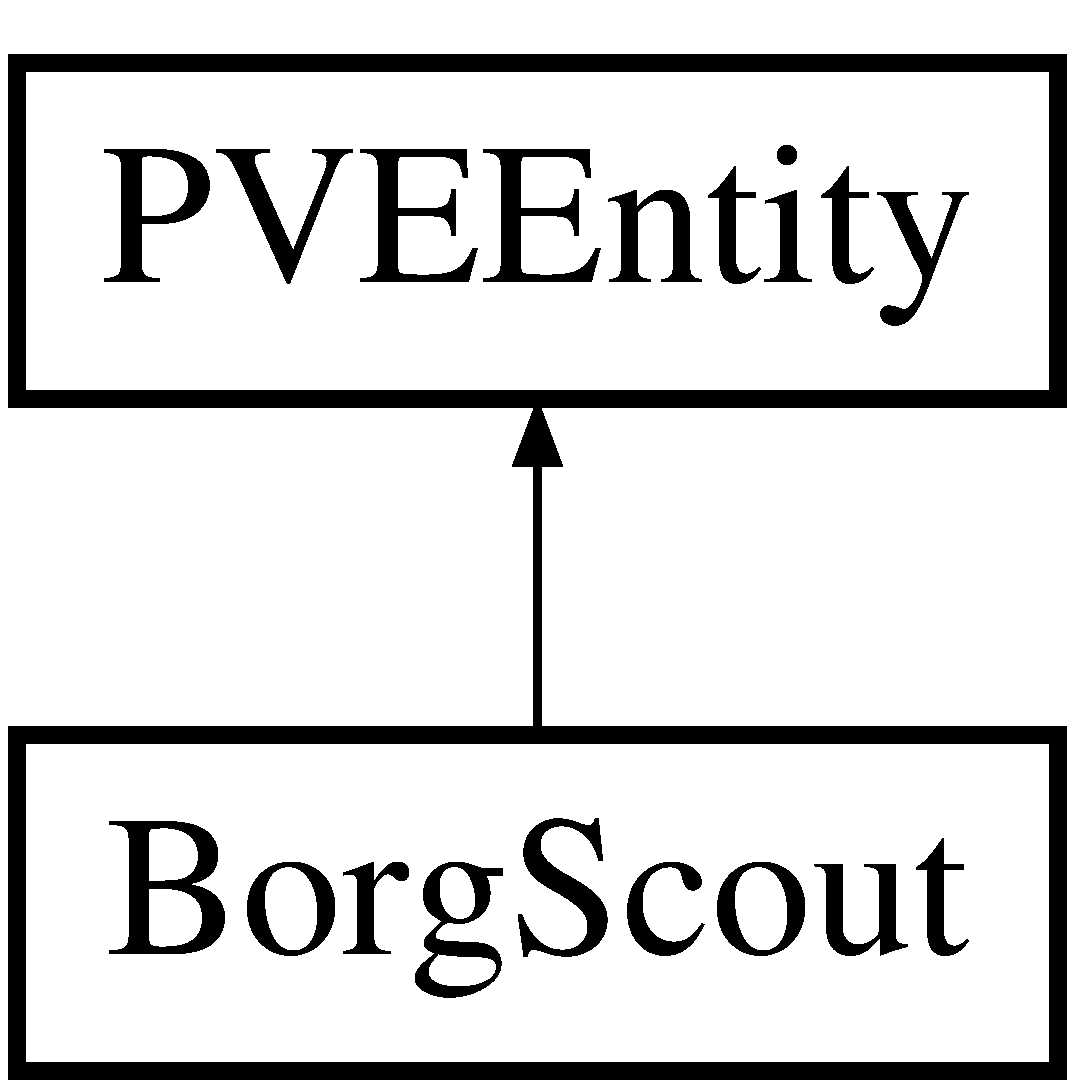
\includegraphics[height=2cm]{d5/d8c/classBorgScout}
\end{center}
\end{figure}
\subsection*{Public Member Functions}
\begin{DoxyCompactItemize}
\item 
\hyperlink{classBorgScout_a4867f3f56ad3f67850e66d89682318a1}{BorgScout} ()
\item 
\hyperlink{classBorgScout_a40f473098c9948cc5bc8df98c1ad58d8}{$\sim$BorgScout} ()
\item 
string \hyperlink{classBorgScout_a59bfebc7126c503bb8f83a5572149e23}{getName} ()
\item 
int \hyperlink{classBorgScout_a083b7b41ca27d5b3f4fa1772f95413e3}{getShieldStrenght} ()
\item 
int \hyperlink{classBorgScout_a7fdb9eda7cced87acb05f9984742da47}{getShieldRegenerativeRate} ()
\item 
int \hyperlink{classBorgScout_af4ab31bd4edc30c887b4a36f9a0f5a62}{getRegenerativeAdaptivePlating} ()
\item 
bool \hyperlink{classBorgScout_a13a50a9d314581a10f232cee3612ce55}{getHasRegenerativeAdaptivePlating} ()
\item 
int \hyperlink{classBorgScout_a88484687d5bbe7616fd2b8f6a705eb34}{getTransPhasicTorpedos} ()
\item 
bool \hyperlink{classBorgScout_a3504b9ab7146069cdda109582f177329}{getHasTransphasicTorpedos} ()
\item 
int \hyperlink{classBorgScout_af4946e931ed104ab99739fb33ca15303}{getChronitonTorpedos} ()
\item 
bool \hyperlink{classBorgScout_a2fe05bd1706ab0f55a8bb3075ab97ca0}{getHasChronitonTorpedos} ()
\item 
int \hyperlink{classBorgScout_a5b025086c5d5f8175df3f9e581a1948e}{getGravimetricTorpedos} ()
\item 
bool \hyperlink{classBorgScout_af9589d7333a7f56aadcd49ebfdb63453}{getHasGravimetricTorpedos} ()
\item 
int \hyperlink{classBorgScout_a7fb32f9bc92f36e05bfb3db42b4b3d91}{getSpatialTorpedos} ()
\item 
bool \hyperlink{classBorgScout_aed0c2eadce9f7ecc0278ccbd139fc795}{getHasSpatialTorpedos} ()
\item 
bool \hyperlink{classBorgScout_a685ff7acbc0f6987cb62a617853f96f7}{getHasLasers} ()
\item 
bool \hyperlink{classBorgScout_a1ee127e8654d327c6ee34b5077c8ea1d}{getHasPhasedIonCannon} ()
\item 
bool \hyperlink{classBorgScout_a4a2dda4639a9f5f53d673cf82d7ff416}{getHasPulseWeapon} ()
\item 
int \hyperlink{classBorgScout_af60afb5ab8fa330ab09a841fe3cc0ae6}{getBorgComplement} ()
\item 
bool \hyperlink{classBorgScout_ac6bc77f2e7232631646afb05b9f706ea}{getHasTractorLock} ()
\item 
bool \hyperlink{classBorgScout_ad904fc2d7473517dc3e9f9a896b1b870}{getIsWreckPVE} ()
\item 
void \hyperlink{classBorgScout_a281c1d904ce2a40d6441b43cafb207c9}{setShieldStrenghtPVE} (int strenght)
\item 
void \hyperlink{classBorgScout_a500ce15b9d01c79a8f7ebefe060b0d6a}{setShieldRegenerativeRatePVE} (int rate)
\item 
void \hyperlink{classBorgScout_ab4cfe88166b8473ec3901afc1f05b462}{setArmourPVE} (int armour)
\item 
void \hyperlink{classBorgScout_aee2837e76125a16bdd56ff967902e99f}{setTransPhasicTorpedosPVE} (int num)
\item 
void \hyperlink{classBorgScout_a82eb31f8b1d94b9ea57cadb97bd276f3}{setChronitonTorpedosPVE} (int num)
\item 
void \hyperlink{classBorgScout_aeb73af88f67173bff2f37138ef8b4b59}{setGravimetricTorpedosPVE} (int num)
\item 
void \hyperlink{classBorgScout_ac911250166eb1fa47f602ead65f7b834}{setSpatialTorpedosPVE} (int num)
\item 
void \hyperlink{classBorgScout_a1d6f8704e2832ef1878d00a2cff6b288}{setHasTractorLockPVE} (bool has)
\item 
void \hyperlink{classBorgScout_ad387c5b9ea86f8e53f6f5ab4cf83bb42}{setWreckPVE} ()
\end{DoxyCompactItemize}


\subsection{Constructor \& Destructor Documentation}
\hypertarget{classBorgScout_a4867f3f56ad3f67850e66d89682318a1}{
\index{BorgScout@{BorgScout}!BorgScout@{BorgScout}}
\index{BorgScout@{BorgScout}!BorgScout@{BorgScout}}
\subsubsection[{BorgScout}]{\setlength{\rightskip}{0pt plus 5cm}BorgScout::BorgScout ()}}
\label{d5/d8c/classBorgScout_a4867f3f56ad3f67850e66d89682318a1}
Constructor for pve entity sets up data embers based on preloaded variables arrays usning random index \hypertarget{classBorgScout_a40f473098c9948cc5bc8df98c1ad58d8}{
\index{BorgScout@{BorgScout}!$\sim$BorgScout@{$\sim$BorgScout}}
\index{$\sim$BorgScout@{$\sim$BorgScout}!BorgScout@{BorgScout}}
\subsubsection[{$\sim$BorgScout}]{\setlength{\rightskip}{0pt plus 5cm}BorgScout::$\sim$BorgScout ()}}
\label{d5/d8c/classBorgScout_a40f473098c9948cc5bc8df98c1ad58d8}
Destructor for the enemy 

\subsection{Member Function Documentation}
\hypertarget{classBorgScout_af60afb5ab8fa330ab09a841fe3cc0ae6}{
\index{BorgScout@{BorgScout}!getBorgComplement@{getBorgComplement}}
\index{getBorgComplement@{getBorgComplement}!BorgScout@{BorgScout}}
\subsubsection[{getBorgComplement}]{\setlength{\rightskip}{0pt plus 5cm}int BorgScout::getBorgComplement ()\hspace{0.3cm}{\ttfamily  \mbox{[}virtual\mbox{]}}}}
\label{d5/d8c/classBorgScout_af60afb5ab8fa330ab09a841fe3cc0ae6}
accessor for the enemies borg complement

\begin{DoxyReturn}{Returns}
int the borg complement data member 
\end{DoxyReturn}


Implements \hyperlink{classPVEEntity}{PVEEntity}.

\hypertarget{classBorgScout_af4946e931ed104ab99739fb33ca15303}{
\index{BorgScout@{BorgScout}!getChronitonTorpedos@{getChronitonTorpedos}}
\index{getChronitonTorpedos@{getChronitonTorpedos}!BorgScout@{BorgScout}}
\subsubsection[{getChronitonTorpedos}]{\setlength{\rightskip}{0pt plus 5cm}int BorgScout::getChronitonTorpedos ()\hspace{0.3cm}{\ttfamily  \mbox{[}virtual\mbox{]}}}}
\label{d5/d8c/classBorgScout_af4946e931ed104ab99739fb33ca15303}
accessor for the enemies chroniton torps

\begin{DoxyReturn}{Returns}
int the chroniton torps data member 
\end{DoxyReturn}


Implements \hyperlink{classPVEEntity}{PVEEntity}.

\hypertarget{classBorgScout_a5b025086c5d5f8175df3f9e581a1948e}{
\index{BorgScout@{BorgScout}!getGravimetricTorpedos@{getGravimetricTorpedos}}
\index{getGravimetricTorpedos@{getGravimetricTorpedos}!BorgScout@{BorgScout}}
\subsubsection[{getGravimetricTorpedos}]{\setlength{\rightskip}{0pt plus 5cm}int BorgScout::getGravimetricTorpedos ()\hspace{0.3cm}{\ttfamily  \mbox{[}virtual\mbox{]}}}}
\label{d5/d8c/classBorgScout_a5b025086c5d5f8175df3f9e581a1948e}
accessor for the enemies gravimetric torps

\begin{DoxyReturn}{Returns}
int the chroniton torps data member 
\end{DoxyReturn}


Implements \hyperlink{classPVEEntity}{PVEEntity}.

\hypertarget{classBorgScout_a2fe05bd1706ab0f55a8bb3075ab97ca0}{
\index{BorgScout@{BorgScout}!getHasChronitonTorpedos@{getHasChronitonTorpedos}}
\index{getHasChronitonTorpedos@{getHasChronitonTorpedos}!BorgScout@{BorgScout}}
\subsubsection[{getHasChronitonTorpedos}]{\setlength{\rightskip}{0pt plus 5cm}bool BorgScout::getHasChronitonTorpedos ()\hspace{0.3cm}{\ttfamily  \mbox{[}virtual\mbox{]}}}}
\label{d5/d8c/classBorgScout_a2fe05bd1706ab0f55a8bb3075ab97ca0}
accessor for the enemies has chroniton torps

\begin{DoxyReturn}{Returns}
bool the has chroniton torps data member 
\end{DoxyReturn}


Implements \hyperlink{classPVEEntity}{PVEEntity}.

\hypertarget{classBorgScout_af9589d7333a7f56aadcd49ebfdb63453}{
\index{BorgScout@{BorgScout}!getHasGravimetricTorpedos@{getHasGravimetricTorpedos}}
\index{getHasGravimetricTorpedos@{getHasGravimetricTorpedos}!BorgScout@{BorgScout}}
\subsubsection[{getHasGravimetricTorpedos}]{\setlength{\rightskip}{0pt plus 5cm}bool BorgScout::getHasGravimetricTorpedos ()\hspace{0.3cm}{\ttfamily  \mbox{[}virtual\mbox{]}}}}
\label{d5/d8c/classBorgScout_af9589d7333a7f56aadcd49ebfdb63453}
accessor for the enemies has gravimetric torps

\begin{DoxyReturn}{Returns}
bool the has chroniton torps data member 
\end{DoxyReturn}


Implements \hyperlink{classPVEEntity}{PVEEntity}.

\hypertarget{classBorgScout_a685ff7acbc0f6987cb62a617853f96f7}{
\index{BorgScout@{BorgScout}!getHasLasers@{getHasLasers}}
\index{getHasLasers@{getHasLasers}!BorgScout@{BorgScout}}
\subsubsection[{getHasLasers}]{\setlength{\rightskip}{0pt plus 5cm}bool BorgScout::getHasLasers ()\hspace{0.3cm}{\ttfamily  \mbox{[}virtual\mbox{]}}}}
\label{d5/d8c/classBorgScout_a685ff7acbc0f6987cb62a617853f96f7}
accessor for the enemies has lasers

\begin{DoxyReturn}{Returns}
bool the has lasers data member 
\end{DoxyReturn}


Implements \hyperlink{classPVEEntity}{PVEEntity}.

\hypertarget{classBorgScout_a1ee127e8654d327c6ee34b5077c8ea1d}{
\index{BorgScout@{BorgScout}!getHasPhasedIonCannon@{getHasPhasedIonCannon}}
\index{getHasPhasedIonCannon@{getHasPhasedIonCannon}!BorgScout@{BorgScout}}
\subsubsection[{getHasPhasedIonCannon}]{\setlength{\rightskip}{0pt plus 5cm}bool BorgScout::getHasPhasedIonCannon ()\hspace{0.3cm}{\ttfamily  \mbox{[}virtual\mbox{]}}}}
\label{d5/d8c/classBorgScout_a1ee127e8654d327c6ee34b5077c8ea1d}
accessor for the enemies has phased ion cannon

\begin{DoxyReturn}{Returns}
bool the has phased ion cannon data member 
\end{DoxyReturn}


Implements \hyperlink{classPVEEntity}{PVEEntity}.

\hypertarget{classBorgScout_a4a2dda4639a9f5f53d673cf82d7ff416}{
\index{BorgScout@{BorgScout}!getHasPulseWeapon@{getHasPulseWeapon}}
\index{getHasPulseWeapon@{getHasPulseWeapon}!BorgScout@{BorgScout}}
\subsubsection[{getHasPulseWeapon}]{\setlength{\rightskip}{0pt plus 5cm}bool BorgScout::getHasPulseWeapon ()\hspace{0.3cm}{\ttfamily  \mbox{[}virtual\mbox{]}}}}
\label{d5/d8c/classBorgScout_a4a2dda4639a9f5f53d673cf82d7ff416}
accessor for the enemies has pulse weapons

\begin{DoxyReturn}{Returns}
bool the has pulse weapons data member 
\end{DoxyReturn}


Implements \hyperlink{classPVEEntity}{PVEEntity}.

\hypertarget{classBorgScout_a13a50a9d314581a10f232cee3612ce55}{
\index{BorgScout@{BorgScout}!getHasRegenerativeAdaptivePlating@{getHasRegenerativeAdaptivePlating}}
\index{getHasRegenerativeAdaptivePlating@{getHasRegenerativeAdaptivePlating}!BorgScout@{BorgScout}}
\subsubsection[{getHasRegenerativeAdaptivePlating}]{\setlength{\rightskip}{0pt plus 5cm}bool BorgScout::getHasRegenerativeAdaptivePlating ()\hspace{0.3cm}{\ttfamily  \mbox{[}virtual\mbox{]}}}}
\label{d5/d8c/classBorgScout_a13a50a9d314581a10f232cee3612ce55}
accessor for the enemies has regenerative adaptive plating

\begin{DoxyReturn}{Returns}
bool the has regenerative adaptive plating data member 
\end{DoxyReturn}


Implements \hyperlink{classPVEEntity}{PVEEntity}.

\hypertarget{classBorgScout_aed0c2eadce9f7ecc0278ccbd139fc795}{
\index{BorgScout@{BorgScout}!getHasSpatialTorpedos@{getHasSpatialTorpedos}}
\index{getHasSpatialTorpedos@{getHasSpatialTorpedos}!BorgScout@{BorgScout}}
\subsubsection[{getHasSpatialTorpedos}]{\setlength{\rightskip}{0pt plus 5cm}bool BorgScout::getHasSpatialTorpedos ()\hspace{0.3cm}{\ttfamily  \mbox{[}virtual\mbox{]}}}}
\label{d5/d8c/classBorgScout_aed0c2eadce9f7ecc0278ccbd139fc795}
accessor for the enemies has spatial torps

\begin{DoxyReturn}{Returns}
bool the has spatial torps data member 
\end{DoxyReturn}


Implements \hyperlink{classPVEEntity}{PVEEntity}.

\hypertarget{classBorgScout_ac6bc77f2e7232631646afb05b9f706ea}{
\index{BorgScout@{BorgScout}!getHasTractorLock@{getHasTractorLock}}
\index{getHasTractorLock@{getHasTractorLock}!BorgScout@{BorgScout}}
\subsubsection[{getHasTractorLock}]{\setlength{\rightskip}{0pt plus 5cm}bool BorgScout::getHasTractorLock ()\hspace{0.3cm}{\ttfamily  \mbox{[}virtual\mbox{]}}}}
\label{d5/d8c/classBorgScout_ac6bc77f2e7232631646afb05b9f706ea}
accessor for the enemies tractor lock

\begin{DoxyReturn}{Returns}
bool the tractor lock data member 
\end{DoxyReturn}


Implements \hyperlink{classPVEEntity}{PVEEntity}.

\hypertarget{classBorgScout_a3504b9ab7146069cdda109582f177329}{
\index{BorgScout@{BorgScout}!getHasTransphasicTorpedos@{getHasTransphasicTorpedos}}
\index{getHasTransphasicTorpedos@{getHasTransphasicTorpedos}!BorgScout@{BorgScout}}
\subsubsection[{getHasTransphasicTorpedos}]{\setlength{\rightskip}{0pt plus 5cm}bool BorgScout::getHasTransphasicTorpedos ()\hspace{0.3cm}{\ttfamily  \mbox{[}virtual\mbox{]}}}}
\label{d5/d8c/classBorgScout_a3504b9ab7146069cdda109582f177329}
accessor for the enemies has transphasic torps

\begin{DoxyReturn}{Returns}
bool the has transphasic torps data member 
\end{DoxyReturn}


Implements \hyperlink{classPVEEntity}{PVEEntity}.

\hypertarget{classBorgScout_ad904fc2d7473517dc3e9f9a896b1b870}{
\index{BorgScout@{BorgScout}!getIsWreckPVE@{getIsWreckPVE}}
\index{getIsWreckPVE@{getIsWreckPVE}!BorgScout@{BorgScout}}
\subsubsection[{getIsWreckPVE}]{\setlength{\rightskip}{0pt plus 5cm}bool BorgScout::getIsWreckPVE ()\hspace{0.3cm}{\ttfamily  \mbox{[}virtual\mbox{]}}}}
\label{d5/d8c/classBorgScout_ad904fc2d7473517dc3e9f9a896b1b870}
accessor for the enemies wreck status

\begin{DoxyReturn}{Returns}
bool the wreck status data member 
\end{DoxyReturn}


Implements \hyperlink{classPVEEntity}{PVEEntity}.

\hypertarget{classBorgScout_a59bfebc7126c503bb8f83a5572149e23}{
\index{BorgScout@{BorgScout}!getName@{getName}}
\index{getName@{getName}!BorgScout@{BorgScout}}
\subsubsection[{getName}]{\setlength{\rightskip}{0pt plus 5cm}string BorgScout::getName ()\hspace{0.3cm}{\ttfamily  \mbox{[}virtual\mbox{]}}}}
\label{d5/d8c/classBorgScout_a59bfebc7126c503bb8f83a5572149e23}
accessor for the enemies name

\begin{DoxyReturn}{Returns}
string the enemies name 
\end{DoxyReturn}


Implements \hyperlink{classPVEEntity}{PVEEntity}.

\hypertarget{classBorgScout_af4ab31bd4edc30c887b4a36f9a0f5a62}{
\index{BorgScout@{BorgScout}!getRegenerativeAdaptivePlating@{getRegenerativeAdaptivePlating}}
\index{getRegenerativeAdaptivePlating@{getRegenerativeAdaptivePlating}!BorgScout@{BorgScout}}
\subsubsection[{getRegenerativeAdaptivePlating}]{\setlength{\rightskip}{0pt plus 5cm}int BorgScout::getRegenerativeAdaptivePlating ()\hspace{0.3cm}{\ttfamily  \mbox{[}virtual\mbox{]}}}}
\label{d5/d8c/classBorgScout_af4ab31bd4edc30c887b4a36f9a0f5a62}
accessor for the enemies regenerative adaptive plating

\begin{DoxyReturn}{Returns}
int the regenerative adaptive plating data member 
\end{DoxyReturn}


Implements \hyperlink{classPVEEntity}{PVEEntity}.

\hypertarget{classBorgScout_a7fdb9eda7cced87acb05f9984742da47}{
\index{BorgScout@{BorgScout}!getShieldRegenerativeRate@{getShieldRegenerativeRate}}
\index{getShieldRegenerativeRate@{getShieldRegenerativeRate}!BorgScout@{BorgScout}}
\subsubsection[{getShieldRegenerativeRate}]{\setlength{\rightskip}{0pt plus 5cm}int BorgScout::getShieldRegenerativeRate ()\hspace{0.3cm}{\ttfamily  \mbox{[}virtual\mbox{]}}}}
\label{d5/d8c/classBorgScout_a7fdb9eda7cced87acb05f9984742da47}
accessor for the enemies shield regenerative rate

\begin{DoxyReturn}{Returns}
int the shield regenerative rate data member 
\end{DoxyReturn}


Implements \hyperlink{classPVEEntity}{PVEEntity}.

\hypertarget{classBorgScout_a083b7b41ca27d5b3f4fa1772f95413e3}{
\index{BorgScout@{BorgScout}!getShieldStrenght@{getShieldStrenght}}
\index{getShieldStrenght@{getShieldStrenght}!BorgScout@{BorgScout}}
\subsubsection[{getShieldStrenght}]{\setlength{\rightskip}{0pt plus 5cm}int BorgScout::getShieldStrenght ()\hspace{0.3cm}{\ttfamily  \mbox{[}virtual\mbox{]}}}}
\label{d5/d8c/classBorgScout_a083b7b41ca27d5b3f4fa1772f95413e3}
accessor for the enemies shield strength

\begin{DoxyReturn}{Returns}
int the shield strength data member 
\end{DoxyReturn}


Implements \hyperlink{classPVEEntity}{PVEEntity}.

\hypertarget{classBorgScout_a7fb32f9bc92f36e05bfb3db42b4b3d91}{
\index{BorgScout@{BorgScout}!getSpatialTorpedos@{getSpatialTorpedos}}
\index{getSpatialTorpedos@{getSpatialTorpedos}!BorgScout@{BorgScout}}
\subsubsection[{getSpatialTorpedos}]{\setlength{\rightskip}{0pt plus 5cm}int BorgScout::getSpatialTorpedos ()\hspace{0.3cm}{\ttfamily  \mbox{[}virtual\mbox{]}}}}
\label{d5/d8c/classBorgScout_a7fb32f9bc92f36e05bfb3db42b4b3d91}
accessor for the enemies spatial torps

\begin{DoxyReturn}{Returns}
int the spatial torps data member 
\end{DoxyReturn}


Implements \hyperlink{classPVEEntity}{PVEEntity}.

\hypertarget{classBorgScout_a88484687d5bbe7616fd2b8f6a705eb34}{
\index{BorgScout@{BorgScout}!getTransPhasicTorpedos@{getTransPhasicTorpedos}}
\index{getTransPhasicTorpedos@{getTransPhasicTorpedos}!BorgScout@{BorgScout}}
\subsubsection[{getTransPhasicTorpedos}]{\setlength{\rightskip}{0pt plus 5cm}int BorgScout::getTransPhasicTorpedos ()\hspace{0.3cm}{\ttfamily  \mbox{[}virtual\mbox{]}}}}
\label{d5/d8c/classBorgScout_a88484687d5bbe7616fd2b8f6a705eb34}
accessor for the enemies has regenerative adaptive plating

\begin{DoxyReturn}{Returns}
bool the has regenerative adaptive plating data member 
\end{DoxyReturn}


Implements \hyperlink{classPVEEntity}{PVEEntity}.

\hypertarget{classBorgScout_ab4cfe88166b8473ec3901afc1f05b462}{
\index{BorgScout@{BorgScout}!setArmourPVE@{setArmourPVE}}
\index{setArmourPVE@{setArmourPVE}!BorgScout@{BorgScout}}
\subsubsection[{setArmourPVE}]{\setlength{\rightskip}{0pt plus 5cm}void BorgScout::setArmourPVE (int {\em armour})\hspace{0.3cm}{\ttfamily  \mbox{[}virtual\mbox{]}}}}
\label{d5/d8c/classBorgScout_ab4cfe88166b8473ec3901afc1f05b462}
mutator for the enemies armour


\begin{DoxyParams}{Parameters}
\item[{\em armour}]the value to set the data member\end{DoxyParams}
\begin{DoxyReturn}{Returns}
void 
\end{DoxyReturn}


Implements \hyperlink{classPVEEntity}{PVEEntity}.

\hypertarget{classBorgScout_a82eb31f8b1d94b9ea57cadb97bd276f3}{
\index{BorgScout@{BorgScout}!setChronitonTorpedosPVE@{setChronitonTorpedosPVE}}
\index{setChronitonTorpedosPVE@{setChronitonTorpedosPVE}!BorgScout@{BorgScout}}
\subsubsection[{setChronitonTorpedosPVE}]{\setlength{\rightskip}{0pt plus 5cm}void BorgScout::setChronitonTorpedosPVE (int {\em num})\hspace{0.3cm}{\ttfamily  \mbox{[}virtual\mbox{]}}}}
\label{d5/d8c/classBorgScout_a82eb31f8b1d94b9ea57cadb97bd276f3}
mutator for the enemies chroniton torps


\begin{DoxyParams}{Parameters}
\item[{\em num}]the value to set the data member\end{DoxyParams}
\begin{DoxyReturn}{Returns}
void 
\end{DoxyReturn}


Implements \hyperlink{classPVEEntity}{PVEEntity}.

\hypertarget{classBorgScout_aeb73af88f67173bff2f37138ef8b4b59}{
\index{BorgScout@{BorgScout}!setGravimetricTorpedosPVE@{setGravimetricTorpedosPVE}}
\index{setGravimetricTorpedosPVE@{setGravimetricTorpedosPVE}!BorgScout@{BorgScout}}
\subsubsection[{setGravimetricTorpedosPVE}]{\setlength{\rightskip}{0pt plus 5cm}void BorgScout::setGravimetricTorpedosPVE (int {\em num})\hspace{0.3cm}{\ttfamily  \mbox{[}virtual\mbox{]}}}}
\label{d5/d8c/classBorgScout_aeb73af88f67173bff2f37138ef8b4b59}
mutator for the enemies gravimetric torps


\begin{DoxyParams}{Parameters}
\item[{\em num}]the value to set the data member\end{DoxyParams}
\begin{DoxyReturn}{Returns}
void 
\end{DoxyReturn}


Implements \hyperlink{classPVEEntity}{PVEEntity}.

\hypertarget{classBorgScout_a1d6f8704e2832ef1878d00a2cff6b288}{
\index{BorgScout@{BorgScout}!setHasTractorLockPVE@{setHasTractorLockPVE}}
\index{setHasTractorLockPVE@{setHasTractorLockPVE}!BorgScout@{BorgScout}}
\subsubsection[{setHasTractorLockPVE}]{\setlength{\rightskip}{0pt plus 5cm}void BorgScout::setHasTractorLockPVE (bool {\em has})\hspace{0.3cm}{\ttfamily  \mbox{[}virtual\mbox{]}}}}
\label{d5/d8c/classBorgScout_a1d6f8704e2832ef1878d00a2cff6b288}
mutator for the enemies tractor beam


\begin{DoxyParams}{Parameters}
\item[{\em has}]the bool value to set the data member\end{DoxyParams}
\begin{DoxyReturn}{Returns}
void 
\end{DoxyReturn}


Implements \hyperlink{classPVEEntity}{PVEEntity}.

\hypertarget{classBorgScout_a500ce15b9d01c79a8f7ebefe060b0d6a}{
\index{BorgScout@{BorgScout}!setShieldRegenerativeRatePVE@{setShieldRegenerativeRatePVE}}
\index{setShieldRegenerativeRatePVE@{setShieldRegenerativeRatePVE}!BorgScout@{BorgScout}}
\subsubsection[{setShieldRegenerativeRatePVE}]{\setlength{\rightskip}{0pt plus 5cm}void BorgScout::setShieldRegenerativeRatePVE (int {\em rate})\hspace{0.3cm}{\ttfamily  \mbox{[}virtual\mbox{]}}}}
\label{d5/d8c/classBorgScout_a500ce15b9d01c79a8f7ebefe060b0d6a}
mutator for the enemies regenerative rate


\begin{DoxyParams}{Parameters}
\item[{\em rate}]the value to set the data member\end{DoxyParams}
\begin{DoxyReturn}{Returns}
void 
\end{DoxyReturn}


Implements \hyperlink{classPVEEntity}{PVEEntity}.

\hypertarget{classBorgScout_a281c1d904ce2a40d6441b43cafb207c9}{
\index{BorgScout@{BorgScout}!setShieldStrenghtPVE@{setShieldStrenghtPVE}}
\index{setShieldStrenghtPVE@{setShieldStrenghtPVE}!BorgScout@{BorgScout}}
\subsubsection[{setShieldStrenghtPVE}]{\setlength{\rightskip}{0pt plus 5cm}void BorgScout::setShieldStrenghtPVE (int {\em strenght})\hspace{0.3cm}{\ttfamily  \mbox{[}virtual\mbox{]}}}}
\label{d5/d8c/classBorgScout_a281c1d904ce2a40d6441b43cafb207c9}
mutator for the enemies shield strength


\begin{DoxyParams}{Parameters}
\item[{\em strenght}]the value to set the data member\end{DoxyParams}
\begin{DoxyReturn}{Returns}
void 
\end{DoxyReturn}


Implements \hyperlink{classPVEEntity}{PVEEntity}.

\hypertarget{classBorgScout_ac911250166eb1fa47f602ead65f7b834}{
\index{BorgScout@{BorgScout}!setSpatialTorpedosPVE@{setSpatialTorpedosPVE}}
\index{setSpatialTorpedosPVE@{setSpatialTorpedosPVE}!BorgScout@{BorgScout}}
\subsubsection[{setSpatialTorpedosPVE}]{\setlength{\rightskip}{0pt plus 5cm}void BorgScout::setSpatialTorpedosPVE (int {\em num})\hspace{0.3cm}{\ttfamily  \mbox{[}virtual\mbox{]}}}}
\label{d5/d8c/classBorgScout_ac911250166eb1fa47f602ead65f7b834}
mutator for the enemies spatial torps


\begin{DoxyParams}{Parameters}
\item[{\em num}]the value to set the data member\end{DoxyParams}
\begin{DoxyReturn}{Returns}
void 
\end{DoxyReturn}


Implements \hyperlink{classPVEEntity}{PVEEntity}.

\hypertarget{classBorgScout_aee2837e76125a16bdd56ff967902e99f}{
\index{BorgScout@{BorgScout}!setTransPhasicTorpedosPVE@{setTransPhasicTorpedosPVE}}
\index{setTransPhasicTorpedosPVE@{setTransPhasicTorpedosPVE}!BorgScout@{BorgScout}}
\subsubsection[{setTransPhasicTorpedosPVE}]{\setlength{\rightskip}{0pt plus 5cm}void BorgScout::setTransPhasicTorpedosPVE (int {\em num})\hspace{0.3cm}{\ttfamily  \mbox{[}virtual\mbox{]}}}}
\label{d5/d8c/classBorgScout_aee2837e76125a16bdd56ff967902e99f}
mutator for the enemies trans phasic torps


\begin{DoxyParams}{Parameters}
\item[{\em num}]the value to set the data member\end{DoxyParams}
\begin{DoxyReturn}{Returns}
void 
\end{DoxyReturn}


Implements \hyperlink{classPVEEntity}{PVEEntity}.

\hypertarget{classBorgScout_ad387c5b9ea86f8e53f6f5ab4cf83bb42}{
\index{BorgScout@{BorgScout}!setWreckPVE@{setWreckPVE}}
\index{setWreckPVE@{setWreckPVE}!BorgScout@{BorgScout}}
\subsubsection[{setWreckPVE}]{\setlength{\rightskip}{0pt plus 5cm}void BorgScout::setWreckPVE ()\hspace{0.3cm}{\ttfamily  \mbox{[}virtual\mbox{]}}}}
\label{d5/d8c/classBorgScout_ad387c5b9ea86f8e53f6f5ab4cf83bb42}
mutator for the enemies wreck state

\begin{DoxyReturn}{Returns}
void 
\end{DoxyReturn}


Implements \hyperlink{classPVEEntity}{PVEEntity}.



The documentation for this class was generated from the following files:\begin{DoxyCompactItemize}
\item 
source/header/BorgScout.h\item 
source/source/BorgScout.cpp\end{DoxyCompactItemize}

\hypertarget{classBorgSphere}{
\section{BorgSphere Class Reference}
\label{d6/ddd/classBorgSphere}\index{BorgSphere@{BorgSphere}}
}
Inheritance diagram for BorgSphere:\begin{figure}[H]
\begin{center}
\leavevmode
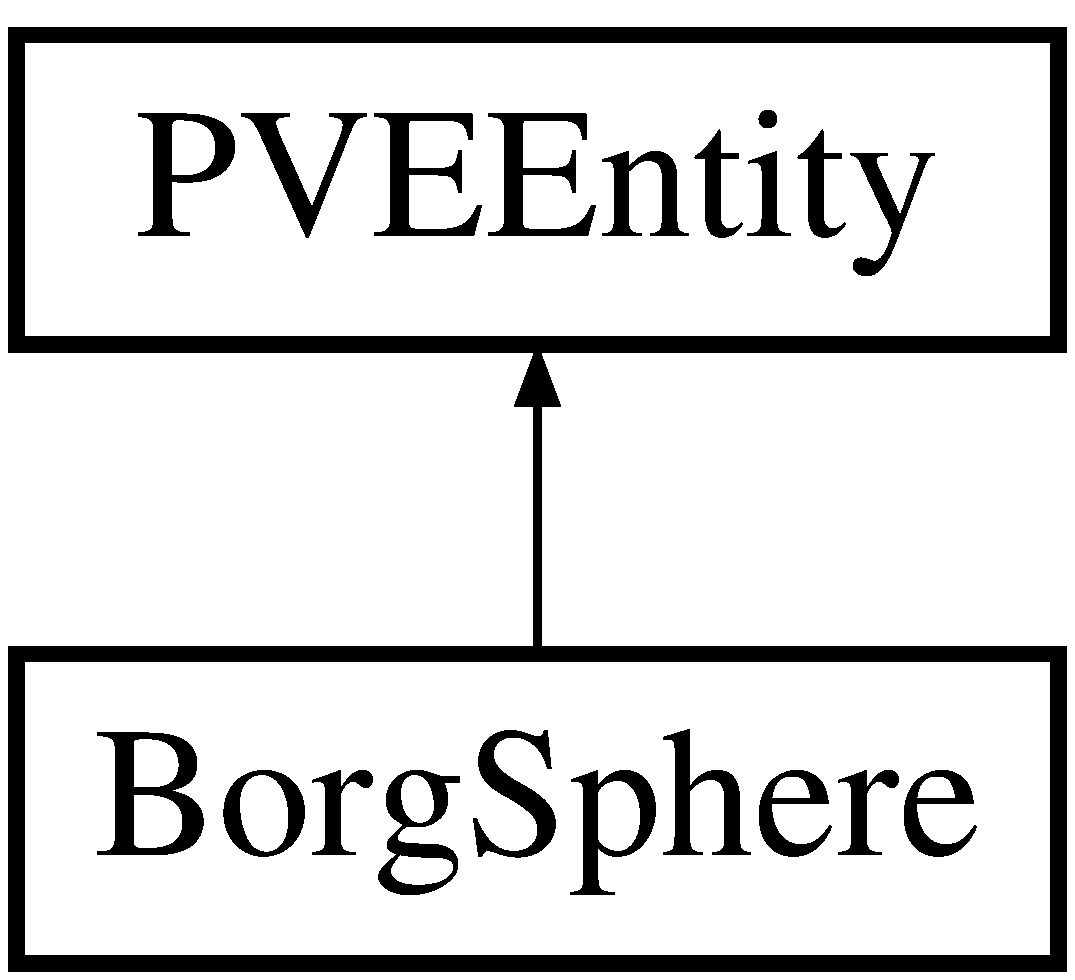
\includegraphics[height=2cm]{d6/ddd/classBorgSphere}
\end{center}
\end{figure}
\subsection*{Public Member Functions}
\begin{DoxyCompactItemize}
\item 
\hyperlink{classBorgSphere_a78ccec8f5d5f1da244b25bec7daebf3a}{BorgSphere} ()
\item 
\hyperlink{classBorgSphere_aa858deaede825f3c2baeddb1cd9fe6a4}{$\sim$BorgSphere} ()
\item 
string \hyperlink{classBorgSphere_a8ff1212f630e7aeb10a6c5249ddd2855}{getName} ()
\item 
int \hyperlink{classBorgSphere_ac67f18e6aa38cf24087411603c3b981f}{getShieldStrenght} ()
\item 
int \hyperlink{classBorgSphere_ac8e9c5b8d9cc105baaa8590171758f9c}{getShieldRegenerativeRate} ()
\item 
int \hyperlink{classBorgSphere_af697ff58376c915ff2bdebad34762296}{getRegenerativeAdaptivePlating} ()
\item 
bool \hyperlink{classBorgSphere_aaf7c47b6913205611bd393345e6264fc}{getHasRegenerativeAdaptivePlating} ()
\item 
int \hyperlink{classBorgSphere_a39fcff670b0233e6ee9eb8b25b723e36}{getTransPhasicTorpedos} ()
\item 
bool \hyperlink{classBorgSphere_a30ef04ddddf5cea157cd73decad5f1c3}{getHasTransphasicTorpedos} ()
\item 
int \hyperlink{classBorgSphere_a2db684357bc18ffcefcb122e70b1034e}{getChronitonTorpedos} ()
\item 
bool \hyperlink{classBorgSphere_a810ef64404ee9a78f8842ef49d998019}{getHasChronitonTorpedos} ()
\item 
int \hyperlink{classBorgSphere_ab6be228e635612baa31385b5f9b7b4f6}{getGravimetricTorpedos} ()
\item 
bool \hyperlink{classBorgSphere_a5c829167ede9b93d7712feed42ebc25c}{getHasGravimetricTorpedos} ()
\item 
int \hyperlink{classBorgSphere_a7cdfa2bc35a23ff6030b2f0071aa0fef}{getSpatialTorpedos} ()
\item 
bool \hyperlink{classBorgSphere_a164d0b9916b378571c2ecf4e2cca604a}{getHasSpatialTorpedos} ()
\item 
bool \hyperlink{classBorgSphere_a1330e8f6c05c6eaf44b601be57d6689a}{getHasLasers} ()
\item 
bool \hyperlink{classBorgSphere_a4fa0c397f2591be8dd30a26fdbf1aa8c}{getHasPhasedIonCannon} ()
\item 
bool \hyperlink{classBorgSphere_a664d07854cf4ccbc82794634946af59f}{getHasPulseWeapon} ()
\item 
int \hyperlink{classBorgSphere_a93dea9d86166e31a47bcce6f57d31b22}{getBorgComplement} ()
\item 
bool \hyperlink{classBorgSphere_aa9ba40319ff0a585222a290e57409891}{getHasTractorLock} ()
\item 
bool \hyperlink{classBorgSphere_a325c849451f5f67ba32d07f93a49a0b0}{getIsWreckPVE} ()
\item 
void \hyperlink{classBorgSphere_a579ab6dc3cb1118ed07a6deb42aa6efa}{setShieldStrenghtPVE} (int strenght)
\item 
void \hyperlink{classBorgSphere_aab1b504e0fd34caae8e74cbe5bddc4dc}{setShieldRegenerativeRatePVE} (int rate)
\item 
void \hyperlink{classBorgSphere_a05cb3b566bae945876f16ba41720746e}{setArmourPVE} (int armour)
\item 
void \hyperlink{classBorgSphere_aabcf70cfb1cb902c44206c6cfb20b159}{setTransPhasicTorpedosPVE} (int num)
\item 
void \hyperlink{classBorgSphere_a46e2416080d4e546645ae88c3a6c47d3}{setChronitonTorpedosPVE} (int num)
\item 
void \hyperlink{classBorgSphere_a9f2faa73e4f5ffee824ac4fa2e66670d}{setGravimetricTorpedosPVE} (int num)
\item 
void \hyperlink{classBorgSphere_a6d1e29d992a4afc48f125e7fff1d89f8}{setSpatialTorpedosPVE} (int num)
\item 
void \hyperlink{classBorgSphere_af53789c3cd02dfb98bfb23e3f91a3822}{setHasTractorLockPVE} (bool has)
\item 
void \hyperlink{classBorgSphere_add9fba918808e2183004ece0a488c854}{setWreckPVE} ()
\end{DoxyCompactItemize}


\subsection{Constructor \& Destructor Documentation}
\hypertarget{classBorgSphere_a78ccec8f5d5f1da244b25bec7daebf3a}{
\index{BorgSphere@{BorgSphere}!BorgSphere@{BorgSphere}}
\index{BorgSphere@{BorgSphere}!BorgSphere@{BorgSphere}}
\subsubsection[{BorgSphere}]{\setlength{\rightskip}{0pt plus 5cm}BorgSphere::BorgSphere ()}}
\label{d6/ddd/classBorgSphere_a78ccec8f5d5f1da244b25bec7daebf3a}
Constructor for pve entity sets up data embers based on preloaded variables arrays usning random index \hypertarget{classBorgSphere_aa858deaede825f3c2baeddb1cd9fe6a4}{
\index{BorgSphere@{BorgSphere}!$\sim$BorgSphere@{$\sim$BorgSphere}}
\index{$\sim$BorgSphere@{$\sim$BorgSphere}!BorgSphere@{BorgSphere}}
\subsubsection[{$\sim$BorgSphere}]{\setlength{\rightskip}{0pt plus 5cm}BorgSphere::$\sim$BorgSphere ()}}
\label{d6/ddd/classBorgSphere_aa858deaede825f3c2baeddb1cd9fe6a4}
Destructor for the enemy 

\subsection{Member Function Documentation}
\hypertarget{classBorgSphere_a93dea9d86166e31a47bcce6f57d31b22}{
\index{BorgSphere@{BorgSphere}!getBorgComplement@{getBorgComplement}}
\index{getBorgComplement@{getBorgComplement}!BorgSphere@{BorgSphere}}
\subsubsection[{getBorgComplement}]{\setlength{\rightskip}{0pt plus 5cm}int BorgSphere::getBorgComplement ()\hspace{0.3cm}{\ttfamily  \mbox{[}virtual\mbox{]}}}}
\label{d6/ddd/classBorgSphere_a93dea9d86166e31a47bcce6f57d31b22}
accessor for the enemies borg complement

\begin{DoxyReturn}{Returns}
int the borg complement data member 
\end{DoxyReturn}


Implements \hyperlink{classPVEEntity}{PVEEntity}.

\hypertarget{classBorgSphere_a2db684357bc18ffcefcb122e70b1034e}{
\index{BorgSphere@{BorgSphere}!getChronitonTorpedos@{getChronitonTorpedos}}
\index{getChronitonTorpedos@{getChronitonTorpedos}!BorgSphere@{BorgSphere}}
\subsubsection[{getChronitonTorpedos}]{\setlength{\rightskip}{0pt plus 5cm}int BorgSphere::getChronitonTorpedos ()\hspace{0.3cm}{\ttfamily  \mbox{[}virtual\mbox{]}}}}
\label{d6/ddd/classBorgSphere_a2db684357bc18ffcefcb122e70b1034e}
accessor for the enemies chroniton torps

\begin{DoxyReturn}{Returns}
int the chroniton torps data member 
\end{DoxyReturn}


Implements \hyperlink{classPVEEntity}{PVEEntity}.

\hypertarget{classBorgSphere_ab6be228e635612baa31385b5f9b7b4f6}{
\index{BorgSphere@{BorgSphere}!getGravimetricTorpedos@{getGravimetricTorpedos}}
\index{getGravimetricTorpedos@{getGravimetricTorpedos}!BorgSphere@{BorgSphere}}
\subsubsection[{getGravimetricTorpedos}]{\setlength{\rightskip}{0pt plus 5cm}int BorgSphere::getGravimetricTorpedos ()\hspace{0.3cm}{\ttfamily  \mbox{[}virtual\mbox{]}}}}
\label{d6/ddd/classBorgSphere_ab6be228e635612baa31385b5f9b7b4f6}
accessor for the enemies gravimetric torps

\begin{DoxyReturn}{Returns}
int the chroniton torps data member 
\end{DoxyReturn}


Implements \hyperlink{classPVEEntity}{PVEEntity}.

\hypertarget{classBorgSphere_a810ef64404ee9a78f8842ef49d998019}{
\index{BorgSphere@{BorgSphere}!getHasChronitonTorpedos@{getHasChronitonTorpedos}}
\index{getHasChronitonTorpedos@{getHasChronitonTorpedos}!BorgSphere@{BorgSphere}}
\subsubsection[{getHasChronitonTorpedos}]{\setlength{\rightskip}{0pt plus 5cm}bool BorgSphere::getHasChronitonTorpedos ()\hspace{0.3cm}{\ttfamily  \mbox{[}virtual\mbox{]}}}}
\label{d6/ddd/classBorgSphere_a810ef64404ee9a78f8842ef49d998019}
accessor for the enemies has chroniton torps

\begin{DoxyReturn}{Returns}
bool the has chroniton torps data member 
\end{DoxyReturn}


Implements \hyperlink{classPVEEntity}{PVEEntity}.

\hypertarget{classBorgSphere_a5c829167ede9b93d7712feed42ebc25c}{
\index{BorgSphere@{BorgSphere}!getHasGravimetricTorpedos@{getHasGravimetricTorpedos}}
\index{getHasGravimetricTorpedos@{getHasGravimetricTorpedos}!BorgSphere@{BorgSphere}}
\subsubsection[{getHasGravimetricTorpedos}]{\setlength{\rightskip}{0pt plus 5cm}bool BorgSphere::getHasGravimetricTorpedos ()\hspace{0.3cm}{\ttfamily  \mbox{[}virtual\mbox{]}}}}
\label{d6/ddd/classBorgSphere_a5c829167ede9b93d7712feed42ebc25c}
accessor for the enemies has gravimetric torps

\begin{DoxyReturn}{Returns}
bool the has chroniton torps data member 
\end{DoxyReturn}


Implements \hyperlink{classPVEEntity}{PVEEntity}.

\hypertarget{classBorgSphere_a1330e8f6c05c6eaf44b601be57d6689a}{
\index{BorgSphere@{BorgSphere}!getHasLasers@{getHasLasers}}
\index{getHasLasers@{getHasLasers}!BorgSphere@{BorgSphere}}
\subsubsection[{getHasLasers}]{\setlength{\rightskip}{0pt plus 5cm}bool BorgSphere::getHasLasers ()\hspace{0.3cm}{\ttfamily  \mbox{[}virtual\mbox{]}}}}
\label{d6/ddd/classBorgSphere_a1330e8f6c05c6eaf44b601be57d6689a}
accessor for the enemies has lasers

\begin{DoxyReturn}{Returns}
bool the has lasers data member 
\end{DoxyReturn}


Implements \hyperlink{classPVEEntity}{PVEEntity}.

\hypertarget{classBorgSphere_a4fa0c397f2591be8dd30a26fdbf1aa8c}{
\index{BorgSphere@{BorgSphere}!getHasPhasedIonCannon@{getHasPhasedIonCannon}}
\index{getHasPhasedIonCannon@{getHasPhasedIonCannon}!BorgSphere@{BorgSphere}}
\subsubsection[{getHasPhasedIonCannon}]{\setlength{\rightskip}{0pt plus 5cm}bool BorgSphere::getHasPhasedIonCannon ()\hspace{0.3cm}{\ttfamily  \mbox{[}virtual\mbox{]}}}}
\label{d6/ddd/classBorgSphere_a4fa0c397f2591be8dd30a26fdbf1aa8c}
accessor for the enemies has phased ion cannon

\begin{DoxyReturn}{Returns}
bool the has phased ion cannon data member 
\end{DoxyReturn}


Implements \hyperlink{classPVEEntity}{PVEEntity}.

\hypertarget{classBorgSphere_a664d07854cf4ccbc82794634946af59f}{
\index{BorgSphere@{BorgSphere}!getHasPulseWeapon@{getHasPulseWeapon}}
\index{getHasPulseWeapon@{getHasPulseWeapon}!BorgSphere@{BorgSphere}}
\subsubsection[{getHasPulseWeapon}]{\setlength{\rightskip}{0pt plus 5cm}bool BorgSphere::getHasPulseWeapon ()\hspace{0.3cm}{\ttfamily  \mbox{[}virtual\mbox{]}}}}
\label{d6/ddd/classBorgSphere_a664d07854cf4ccbc82794634946af59f}
accessor for the enemies has pulse weapons

\begin{DoxyReturn}{Returns}
bool the has pulse weapons data member 
\end{DoxyReturn}


Implements \hyperlink{classPVEEntity}{PVEEntity}.

\hypertarget{classBorgSphere_aaf7c47b6913205611bd393345e6264fc}{
\index{BorgSphere@{BorgSphere}!getHasRegenerativeAdaptivePlating@{getHasRegenerativeAdaptivePlating}}
\index{getHasRegenerativeAdaptivePlating@{getHasRegenerativeAdaptivePlating}!BorgSphere@{BorgSphere}}
\subsubsection[{getHasRegenerativeAdaptivePlating}]{\setlength{\rightskip}{0pt plus 5cm}bool BorgSphere::getHasRegenerativeAdaptivePlating ()\hspace{0.3cm}{\ttfamily  \mbox{[}virtual\mbox{]}}}}
\label{d6/ddd/classBorgSphere_aaf7c47b6913205611bd393345e6264fc}
accessor for the enemies has regenerative adaptive plating

\begin{DoxyReturn}{Returns}
bool the has regenerative adaptive plating data member 
\end{DoxyReturn}


Implements \hyperlink{classPVEEntity}{PVEEntity}.

\hypertarget{classBorgSphere_a164d0b9916b378571c2ecf4e2cca604a}{
\index{BorgSphere@{BorgSphere}!getHasSpatialTorpedos@{getHasSpatialTorpedos}}
\index{getHasSpatialTorpedos@{getHasSpatialTorpedos}!BorgSphere@{BorgSphere}}
\subsubsection[{getHasSpatialTorpedos}]{\setlength{\rightskip}{0pt plus 5cm}bool BorgSphere::getHasSpatialTorpedos ()\hspace{0.3cm}{\ttfamily  \mbox{[}virtual\mbox{]}}}}
\label{d6/ddd/classBorgSphere_a164d0b9916b378571c2ecf4e2cca604a}
accessor for the enemies has spatial torps

\begin{DoxyReturn}{Returns}
bool the has spatial torps data member 
\end{DoxyReturn}


Implements \hyperlink{classPVEEntity}{PVEEntity}.

\hypertarget{classBorgSphere_aa9ba40319ff0a585222a290e57409891}{
\index{BorgSphere@{BorgSphere}!getHasTractorLock@{getHasTractorLock}}
\index{getHasTractorLock@{getHasTractorLock}!BorgSphere@{BorgSphere}}
\subsubsection[{getHasTractorLock}]{\setlength{\rightskip}{0pt plus 5cm}bool BorgSphere::getHasTractorLock ()\hspace{0.3cm}{\ttfamily  \mbox{[}virtual\mbox{]}}}}
\label{d6/ddd/classBorgSphere_aa9ba40319ff0a585222a290e57409891}
accessor for the enemies tractor lock

\begin{DoxyReturn}{Returns}
bool the tractor lock data member 
\end{DoxyReturn}


Implements \hyperlink{classPVEEntity}{PVEEntity}.

\hypertarget{classBorgSphere_a30ef04ddddf5cea157cd73decad5f1c3}{
\index{BorgSphere@{BorgSphere}!getHasTransphasicTorpedos@{getHasTransphasicTorpedos}}
\index{getHasTransphasicTorpedos@{getHasTransphasicTorpedos}!BorgSphere@{BorgSphere}}
\subsubsection[{getHasTransphasicTorpedos}]{\setlength{\rightskip}{0pt plus 5cm}bool BorgSphere::getHasTransphasicTorpedos ()\hspace{0.3cm}{\ttfamily  \mbox{[}virtual\mbox{]}}}}
\label{d6/ddd/classBorgSphere_a30ef04ddddf5cea157cd73decad5f1c3}
accessor for the enemies has transphasic torps

\begin{DoxyReturn}{Returns}
bool the has transphasic torps data member 
\end{DoxyReturn}


Implements \hyperlink{classPVEEntity}{PVEEntity}.

\hypertarget{classBorgSphere_a325c849451f5f67ba32d07f93a49a0b0}{
\index{BorgSphere@{BorgSphere}!getIsWreckPVE@{getIsWreckPVE}}
\index{getIsWreckPVE@{getIsWreckPVE}!BorgSphere@{BorgSphere}}
\subsubsection[{getIsWreckPVE}]{\setlength{\rightskip}{0pt plus 5cm}bool BorgSphere::getIsWreckPVE ()\hspace{0.3cm}{\ttfamily  \mbox{[}virtual\mbox{]}}}}
\label{d6/ddd/classBorgSphere_a325c849451f5f67ba32d07f93a49a0b0}
accessor for the enemies wreck status

\begin{DoxyReturn}{Returns}
bool the wreck status data member 
\end{DoxyReturn}


Implements \hyperlink{classPVEEntity}{PVEEntity}.

\hypertarget{classBorgSphere_a8ff1212f630e7aeb10a6c5249ddd2855}{
\index{BorgSphere@{BorgSphere}!getName@{getName}}
\index{getName@{getName}!BorgSphere@{BorgSphere}}
\subsubsection[{getName}]{\setlength{\rightskip}{0pt plus 5cm}string BorgSphere::getName ()\hspace{0.3cm}{\ttfamily  \mbox{[}virtual\mbox{]}}}}
\label{d6/ddd/classBorgSphere_a8ff1212f630e7aeb10a6c5249ddd2855}
accessor for the enemies name

\begin{DoxyReturn}{Returns}
string the enemies name 
\end{DoxyReturn}


Implements \hyperlink{classPVEEntity}{PVEEntity}.

\hypertarget{classBorgSphere_af697ff58376c915ff2bdebad34762296}{
\index{BorgSphere@{BorgSphere}!getRegenerativeAdaptivePlating@{getRegenerativeAdaptivePlating}}
\index{getRegenerativeAdaptivePlating@{getRegenerativeAdaptivePlating}!BorgSphere@{BorgSphere}}
\subsubsection[{getRegenerativeAdaptivePlating}]{\setlength{\rightskip}{0pt plus 5cm}int BorgSphere::getRegenerativeAdaptivePlating ()\hspace{0.3cm}{\ttfamily  \mbox{[}virtual\mbox{]}}}}
\label{d6/ddd/classBorgSphere_af697ff58376c915ff2bdebad34762296}
accessor for the enemies regenerative adaptive plating

\begin{DoxyReturn}{Returns}
int the regenerative adaptive plating data member 
\end{DoxyReturn}


Implements \hyperlink{classPVEEntity}{PVEEntity}.

\hypertarget{classBorgSphere_ac8e9c5b8d9cc105baaa8590171758f9c}{
\index{BorgSphere@{BorgSphere}!getShieldRegenerativeRate@{getShieldRegenerativeRate}}
\index{getShieldRegenerativeRate@{getShieldRegenerativeRate}!BorgSphere@{BorgSphere}}
\subsubsection[{getShieldRegenerativeRate}]{\setlength{\rightskip}{0pt plus 5cm}int BorgSphere::getShieldRegenerativeRate ()\hspace{0.3cm}{\ttfamily  \mbox{[}virtual\mbox{]}}}}
\label{d6/ddd/classBorgSphere_ac8e9c5b8d9cc105baaa8590171758f9c}
accessor for the enemies shield regenerative rate

\begin{DoxyReturn}{Returns}
int the shield regenerative rate data member 
\end{DoxyReturn}


Implements \hyperlink{classPVEEntity}{PVEEntity}.

\hypertarget{classBorgSphere_ac67f18e6aa38cf24087411603c3b981f}{
\index{BorgSphere@{BorgSphere}!getShieldStrenght@{getShieldStrenght}}
\index{getShieldStrenght@{getShieldStrenght}!BorgSphere@{BorgSphere}}
\subsubsection[{getShieldStrenght}]{\setlength{\rightskip}{0pt plus 5cm}int BorgSphere::getShieldStrenght ()\hspace{0.3cm}{\ttfamily  \mbox{[}virtual\mbox{]}}}}
\label{d6/ddd/classBorgSphere_ac67f18e6aa38cf24087411603c3b981f}
accessor for the enemies shield strength

\begin{DoxyReturn}{Returns}
int the shield strength data member 
\end{DoxyReturn}


Implements \hyperlink{classPVEEntity}{PVEEntity}.

\hypertarget{classBorgSphere_a7cdfa2bc35a23ff6030b2f0071aa0fef}{
\index{BorgSphere@{BorgSphere}!getSpatialTorpedos@{getSpatialTorpedos}}
\index{getSpatialTorpedos@{getSpatialTorpedos}!BorgSphere@{BorgSphere}}
\subsubsection[{getSpatialTorpedos}]{\setlength{\rightskip}{0pt plus 5cm}int BorgSphere::getSpatialTorpedos ()\hspace{0.3cm}{\ttfamily  \mbox{[}virtual\mbox{]}}}}
\label{d6/ddd/classBorgSphere_a7cdfa2bc35a23ff6030b2f0071aa0fef}
accessor for the enemies spatial torps

\begin{DoxyReturn}{Returns}
int the spatial torps data member 
\end{DoxyReturn}


Implements \hyperlink{classPVEEntity}{PVEEntity}.

\hypertarget{classBorgSphere_a39fcff670b0233e6ee9eb8b25b723e36}{
\index{BorgSphere@{BorgSphere}!getTransPhasicTorpedos@{getTransPhasicTorpedos}}
\index{getTransPhasicTorpedos@{getTransPhasicTorpedos}!BorgSphere@{BorgSphere}}
\subsubsection[{getTransPhasicTorpedos}]{\setlength{\rightskip}{0pt plus 5cm}int BorgSphere::getTransPhasicTorpedos ()\hspace{0.3cm}{\ttfamily  \mbox{[}virtual\mbox{]}}}}
\label{d6/ddd/classBorgSphere_a39fcff670b0233e6ee9eb8b25b723e36}
accessor for the enemies has regenerative adaptive plating

\begin{DoxyReturn}{Returns}
bool the has regenerative adaptive plating data member 
\end{DoxyReturn}


Implements \hyperlink{classPVEEntity}{PVEEntity}.

\hypertarget{classBorgSphere_a05cb3b566bae945876f16ba41720746e}{
\index{BorgSphere@{BorgSphere}!setArmourPVE@{setArmourPVE}}
\index{setArmourPVE@{setArmourPVE}!BorgSphere@{BorgSphere}}
\subsubsection[{setArmourPVE}]{\setlength{\rightskip}{0pt plus 5cm}void BorgSphere::setArmourPVE (int {\em armour})\hspace{0.3cm}{\ttfamily  \mbox{[}virtual\mbox{]}}}}
\label{d6/ddd/classBorgSphere_a05cb3b566bae945876f16ba41720746e}
mutator for the enemies armour


\begin{DoxyParams}{Parameters}
\item[{\em armour}]the value to set the data member\end{DoxyParams}
\begin{DoxyReturn}{Returns}
void 
\end{DoxyReturn}


Implements \hyperlink{classPVEEntity}{PVEEntity}.

\hypertarget{classBorgSphere_a46e2416080d4e546645ae88c3a6c47d3}{
\index{BorgSphere@{BorgSphere}!setChronitonTorpedosPVE@{setChronitonTorpedosPVE}}
\index{setChronitonTorpedosPVE@{setChronitonTorpedosPVE}!BorgSphere@{BorgSphere}}
\subsubsection[{setChronitonTorpedosPVE}]{\setlength{\rightskip}{0pt plus 5cm}void BorgSphere::setChronitonTorpedosPVE (int {\em num})\hspace{0.3cm}{\ttfamily  \mbox{[}virtual\mbox{]}}}}
\label{d6/ddd/classBorgSphere_a46e2416080d4e546645ae88c3a6c47d3}
mutator for the enemies chroniton torps


\begin{DoxyParams}{Parameters}
\item[{\em num}]the value to set the data member\end{DoxyParams}
\begin{DoxyReturn}{Returns}
void 
\end{DoxyReturn}


Implements \hyperlink{classPVEEntity}{PVEEntity}.

\hypertarget{classBorgSphere_a9f2faa73e4f5ffee824ac4fa2e66670d}{
\index{BorgSphere@{BorgSphere}!setGravimetricTorpedosPVE@{setGravimetricTorpedosPVE}}
\index{setGravimetricTorpedosPVE@{setGravimetricTorpedosPVE}!BorgSphere@{BorgSphere}}
\subsubsection[{setGravimetricTorpedosPVE}]{\setlength{\rightskip}{0pt plus 5cm}void BorgSphere::setGravimetricTorpedosPVE (int {\em num})\hspace{0.3cm}{\ttfamily  \mbox{[}virtual\mbox{]}}}}
\label{d6/ddd/classBorgSphere_a9f2faa73e4f5ffee824ac4fa2e66670d}
mutator for the enemies gravimetric torps


\begin{DoxyParams}{Parameters}
\item[{\em num}]the value to set the data member\end{DoxyParams}
\begin{DoxyReturn}{Returns}
void 
\end{DoxyReturn}


Implements \hyperlink{classPVEEntity}{PVEEntity}.

\hypertarget{classBorgSphere_af53789c3cd02dfb98bfb23e3f91a3822}{
\index{BorgSphere@{BorgSphere}!setHasTractorLockPVE@{setHasTractorLockPVE}}
\index{setHasTractorLockPVE@{setHasTractorLockPVE}!BorgSphere@{BorgSphere}}
\subsubsection[{setHasTractorLockPVE}]{\setlength{\rightskip}{0pt plus 5cm}void BorgSphere::setHasTractorLockPVE (bool {\em has})\hspace{0.3cm}{\ttfamily  \mbox{[}virtual\mbox{]}}}}
\label{d6/ddd/classBorgSphere_af53789c3cd02dfb98bfb23e3f91a3822}
mutator for the enemies tractor beam


\begin{DoxyParams}{Parameters}
\item[{\em has}]the bool value to set the data member\end{DoxyParams}
\begin{DoxyReturn}{Returns}
void 
\end{DoxyReturn}


Implements \hyperlink{classPVEEntity}{PVEEntity}.

\hypertarget{classBorgSphere_aab1b504e0fd34caae8e74cbe5bddc4dc}{
\index{BorgSphere@{BorgSphere}!setShieldRegenerativeRatePVE@{setShieldRegenerativeRatePVE}}
\index{setShieldRegenerativeRatePVE@{setShieldRegenerativeRatePVE}!BorgSphere@{BorgSphere}}
\subsubsection[{setShieldRegenerativeRatePVE}]{\setlength{\rightskip}{0pt plus 5cm}void BorgSphere::setShieldRegenerativeRatePVE (int {\em rate})\hspace{0.3cm}{\ttfamily  \mbox{[}virtual\mbox{]}}}}
\label{d6/ddd/classBorgSphere_aab1b504e0fd34caae8e74cbe5bddc4dc}
mutator for the enemies regenerative rate


\begin{DoxyParams}{Parameters}
\item[{\em rate}]the value to set the data member\end{DoxyParams}
\begin{DoxyReturn}{Returns}
void 
\end{DoxyReturn}


Implements \hyperlink{classPVEEntity}{PVEEntity}.

\hypertarget{classBorgSphere_a579ab6dc3cb1118ed07a6deb42aa6efa}{
\index{BorgSphere@{BorgSphere}!setShieldStrenghtPVE@{setShieldStrenghtPVE}}
\index{setShieldStrenghtPVE@{setShieldStrenghtPVE}!BorgSphere@{BorgSphere}}
\subsubsection[{setShieldStrenghtPVE}]{\setlength{\rightskip}{0pt plus 5cm}void BorgSphere::setShieldStrenghtPVE (int {\em strenght})\hspace{0.3cm}{\ttfamily  \mbox{[}virtual\mbox{]}}}}
\label{d6/ddd/classBorgSphere_a579ab6dc3cb1118ed07a6deb42aa6efa}
mutator for the enemies shield strength


\begin{DoxyParams}{Parameters}
\item[{\em strenght}]the value to set the data member\end{DoxyParams}
\begin{DoxyReturn}{Returns}
void 
\end{DoxyReturn}


Implements \hyperlink{classPVEEntity}{PVEEntity}.

\hypertarget{classBorgSphere_a6d1e29d992a4afc48f125e7fff1d89f8}{
\index{BorgSphere@{BorgSphere}!setSpatialTorpedosPVE@{setSpatialTorpedosPVE}}
\index{setSpatialTorpedosPVE@{setSpatialTorpedosPVE}!BorgSphere@{BorgSphere}}
\subsubsection[{setSpatialTorpedosPVE}]{\setlength{\rightskip}{0pt plus 5cm}void BorgSphere::setSpatialTorpedosPVE (int {\em num})\hspace{0.3cm}{\ttfamily  \mbox{[}virtual\mbox{]}}}}
\label{d6/ddd/classBorgSphere_a6d1e29d992a4afc48f125e7fff1d89f8}
mutator for the enemies spatial torps


\begin{DoxyParams}{Parameters}
\item[{\em num}]the value to set the data member\end{DoxyParams}
\begin{DoxyReturn}{Returns}
void 
\end{DoxyReturn}


Implements \hyperlink{classPVEEntity}{PVEEntity}.

\hypertarget{classBorgSphere_aabcf70cfb1cb902c44206c6cfb20b159}{
\index{BorgSphere@{BorgSphere}!setTransPhasicTorpedosPVE@{setTransPhasicTorpedosPVE}}
\index{setTransPhasicTorpedosPVE@{setTransPhasicTorpedosPVE}!BorgSphere@{BorgSphere}}
\subsubsection[{setTransPhasicTorpedosPVE}]{\setlength{\rightskip}{0pt plus 5cm}void BorgSphere::setTransPhasicTorpedosPVE (int {\em num})\hspace{0.3cm}{\ttfamily  \mbox{[}virtual\mbox{]}}}}
\label{d6/ddd/classBorgSphere_aabcf70cfb1cb902c44206c6cfb20b159}
mutator for the enemies trans phasic torps


\begin{DoxyParams}{Parameters}
\item[{\em num}]the value to set the data member\end{DoxyParams}
\begin{DoxyReturn}{Returns}
void 
\end{DoxyReturn}


Implements \hyperlink{classPVEEntity}{PVEEntity}.

\hypertarget{classBorgSphere_add9fba918808e2183004ece0a488c854}{
\index{BorgSphere@{BorgSphere}!setWreckPVE@{setWreckPVE}}
\index{setWreckPVE@{setWreckPVE}!BorgSphere@{BorgSphere}}
\subsubsection[{setWreckPVE}]{\setlength{\rightskip}{0pt plus 5cm}void BorgSphere::setWreckPVE ()\hspace{0.3cm}{\ttfamily  \mbox{[}virtual\mbox{]}}}}
\label{d6/ddd/classBorgSphere_add9fba918808e2183004ece0a488c854}
mutator for the enemies wreck state

\begin{DoxyReturn}{Returns}
void 
\end{DoxyReturn}


Implements \hyperlink{classPVEEntity}{PVEEntity}.



The documentation for this class was generated from the following files:\begin{DoxyCompactItemize}
\item 
source/header/BorgSphere.h\item 
source/source/BorgSphere.cpp\end{DoxyCompactItemize}

\hypertarget{classBorgTactical}{
\section{BorgTactical Class Reference}
\label{d0/d4e/classBorgTactical}\index{BorgTactical@{BorgTactical}}
}
Inheritance diagram for BorgTactical:\begin{figure}[H]
\begin{center}
\leavevmode
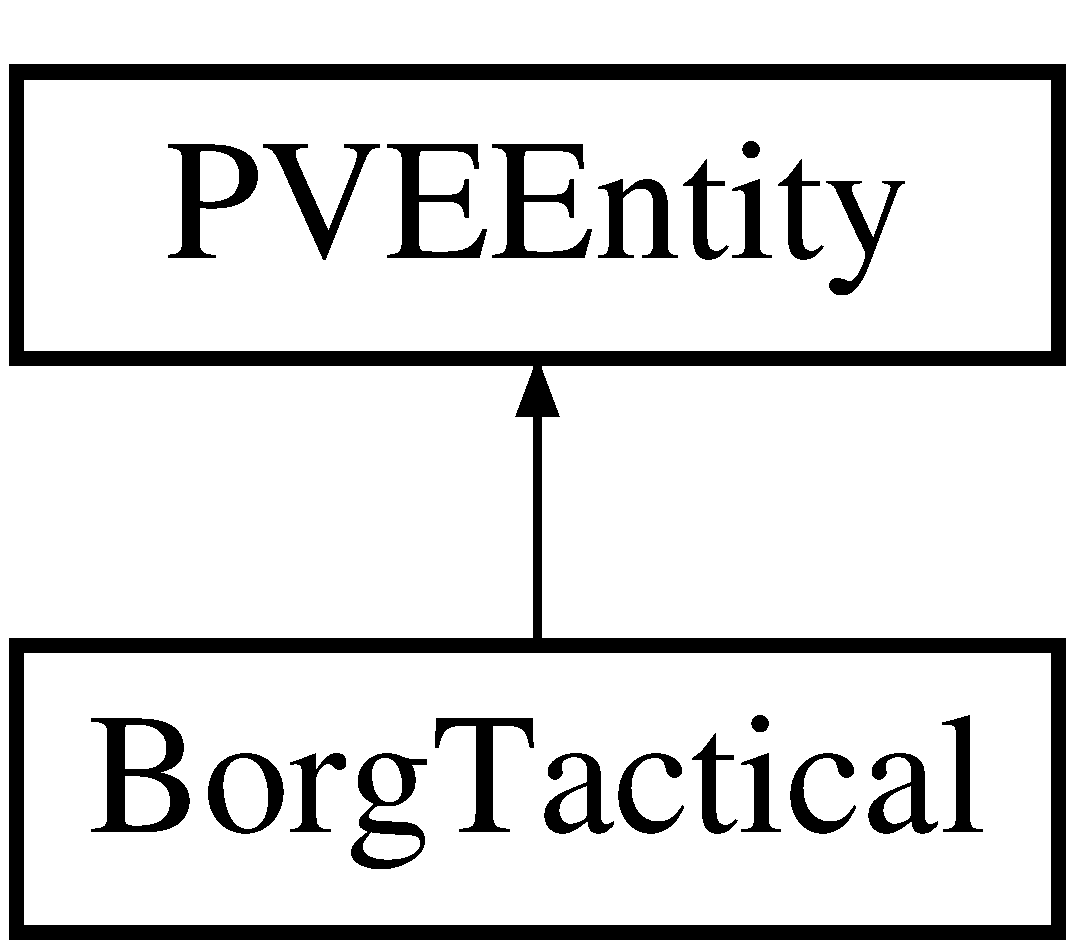
\includegraphics[height=2cm]{d0/d4e/classBorgTactical}
\end{center}
\end{figure}
\subsection*{Public Member Functions}
\begin{DoxyCompactItemize}
\item 
\hyperlink{classBorgTactical_ac4cf305eefa102b5a09ad6f8c12276c2}{BorgTactical} ()
\item 
\hyperlink{classBorgTactical_a33dadcd0fdae2e7342f37b932ac153e2}{$\sim$BorgTactical} ()
\item 
string \hyperlink{classBorgTactical_a456907d48bdd59c8300d9087ba99e1fb}{getName} ()
\item 
int \hyperlink{classBorgTactical_add906680b27f10814a90871df6b7a5bf}{getShieldStrenght} ()
\item 
int \hyperlink{classBorgTactical_a6695595b8993d01254cbe36676ddfb5a}{getShieldRegenerativeRate} ()
\item 
int \hyperlink{classBorgTactical_a2a2943c732727f0d80c63500b5ca527c}{getRegenerativeAdaptivePlating} ()
\item 
bool \hyperlink{classBorgTactical_ade29b0b43b95245653b98f2c0404e782}{getHasRegenerativeAdaptivePlating} ()
\item 
int \hyperlink{classBorgTactical_aa1b3f168acdd21317a4722a29f141bbd}{getTransPhasicTorpedos} ()
\item 
bool \hyperlink{classBorgTactical_a6e551bf387d323403ec3101a97f69501}{getHasTransphasicTorpedos} ()
\item 
int \hyperlink{classBorgTactical_a7ec4b30da34f8218af05f3b6f8edae7a}{getChronitonTorpedos} ()
\item 
bool \hyperlink{classBorgTactical_a8935e0a04c713ffe97bd2174cd07e378}{getHasChronitonTorpedos} ()
\item 
int \hyperlink{classBorgTactical_a8fe417f1c8ae45dbef3c47799c53ed67}{getGravimetricTorpedos} ()
\item 
bool \hyperlink{classBorgTactical_a9d6b52ebb37608db2a10fd7f690a1103}{getHasGravimetricTorpedos} ()
\item 
int \hyperlink{classBorgTactical_a2809be98aae522a10adffabe2a118001}{getSpatialTorpedos} ()
\item 
bool \hyperlink{classBorgTactical_a3bdb9af44e6b4e0f82786ea56ffb4886}{getHasSpatialTorpedos} ()
\item 
bool \hyperlink{classBorgTactical_a8259fa23b1207cd31564bfd1e30781e5}{getHasLasers} ()
\item 
bool \hyperlink{classBorgTactical_ab8ebb12c13c99f80d20fc829298fd05e}{getHasPhasedIonCannon} ()
\item 
bool \hyperlink{classBorgTactical_af5ccad2e38ebe5fded20b3a455bb88ce}{getHasPulseWeapon} ()
\item 
int \hyperlink{classBorgTactical_a71200942186755926d8314658eb06ad5}{getBorgComplement} ()
\item 
bool \hyperlink{classBorgTactical_aa9757380ba5e1f4968fd7a817c464bae}{getHasTractorLock} ()
\item 
bool \hyperlink{classBorgTactical_af53bed854ce027b8e657fa58f8cbda9a}{getIsWreckPVE} ()
\item 
void \hyperlink{classBorgTactical_a193a199b54952f5bdae9d567402a35ba}{setShieldStrenghtPVE} (int strenght)
\item 
void \hyperlink{classBorgTactical_a65e3232f49c6f8c3e318c4e3626f926c}{setShieldRegenerativeRatePVE} (int rate)
\item 
void \hyperlink{classBorgTactical_a1981835f6fd3b9f4cd8b98de13db73fd}{setArmourPVE} (int armour)
\item 
void \hyperlink{classBorgTactical_a4167123bef0b0fa986c180592cb6d729}{setTransPhasicTorpedosPVE} (int num)
\item 
void \hyperlink{classBorgTactical_ad96d089c1faa7171175621aaa2861dfa}{setChronitonTorpedosPVE} (int num)
\item 
void \hyperlink{classBorgTactical_ac2c1e7ad4fc13eb3ea9c47adf9532092}{setGravimetricTorpedosPVE} (int num)
\item 
void \hyperlink{classBorgTactical_a9266ebc1f9df7c6e970537928d2211db}{setSpatialTorpedosPVE} (int num)
\item 
void \hyperlink{classBorgTactical_a57b590444887110e9f09915413a62aaf}{setHasTractorLockPVE} (bool has)
\item 
void \hyperlink{classBorgTactical_a46369732b46f077b30b9c5616755e747}{setWreckPVE} ()
\end{DoxyCompactItemize}


\subsection{Constructor \& Destructor Documentation}
\hypertarget{classBorgTactical_ac4cf305eefa102b5a09ad6f8c12276c2}{
\index{BorgTactical@{BorgTactical}!BorgTactical@{BorgTactical}}
\index{BorgTactical@{BorgTactical}!BorgTactical@{BorgTactical}}
\subsubsection[{BorgTactical}]{\setlength{\rightskip}{0pt plus 5cm}BorgTactical::BorgTactical ()}}
\label{d0/d4e/classBorgTactical_ac4cf305eefa102b5a09ad6f8c12276c2}
Constructor for pve entity sets up data embers based on preloaded variables arrays usning random index \hypertarget{classBorgTactical_a33dadcd0fdae2e7342f37b932ac153e2}{
\index{BorgTactical@{BorgTactical}!$\sim$BorgTactical@{$\sim$BorgTactical}}
\index{$\sim$BorgTactical@{$\sim$BorgTactical}!BorgTactical@{BorgTactical}}
\subsubsection[{$\sim$BorgTactical}]{\setlength{\rightskip}{0pt plus 5cm}BorgTactical::$\sim$BorgTactical ()}}
\label{d0/d4e/classBorgTactical_a33dadcd0fdae2e7342f37b932ac153e2}
Destructor for the enemy 

\subsection{Member Function Documentation}
\hypertarget{classBorgTactical_a71200942186755926d8314658eb06ad5}{
\index{BorgTactical@{BorgTactical}!getBorgComplement@{getBorgComplement}}
\index{getBorgComplement@{getBorgComplement}!BorgTactical@{BorgTactical}}
\subsubsection[{getBorgComplement}]{\setlength{\rightskip}{0pt plus 5cm}int BorgTactical::getBorgComplement ()\hspace{0.3cm}{\ttfamily  \mbox{[}virtual\mbox{]}}}}
\label{d0/d4e/classBorgTactical_a71200942186755926d8314658eb06ad5}
accessor for the enemies borg complement

\begin{DoxyReturn}{Returns}
int the borg complement data member 
\end{DoxyReturn}


Implements \hyperlink{classPVEEntity}{PVEEntity}.

\hypertarget{classBorgTactical_a7ec4b30da34f8218af05f3b6f8edae7a}{
\index{BorgTactical@{BorgTactical}!getChronitonTorpedos@{getChronitonTorpedos}}
\index{getChronitonTorpedos@{getChronitonTorpedos}!BorgTactical@{BorgTactical}}
\subsubsection[{getChronitonTorpedos}]{\setlength{\rightskip}{0pt plus 5cm}int BorgTactical::getChronitonTorpedos ()\hspace{0.3cm}{\ttfamily  \mbox{[}virtual\mbox{]}}}}
\label{d0/d4e/classBorgTactical_a7ec4b30da34f8218af05f3b6f8edae7a}
accessor for the enemies chroniton torps

\begin{DoxyReturn}{Returns}
int the chroniton torps data member 
\end{DoxyReturn}


Implements \hyperlink{classPVEEntity}{PVEEntity}.

\hypertarget{classBorgTactical_a8fe417f1c8ae45dbef3c47799c53ed67}{
\index{BorgTactical@{BorgTactical}!getGravimetricTorpedos@{getGravimetricTorpedos}}
\index{getGravimetricTorpedos@{getGravimetricTorpedos}!BorgTactical@{BorgTactical}}
\subsubsection[{getGravimetricTorpedos}]{\setlength{\rightskip}{0pt plus 5cm}int BorgTactical::getGravimetricTorpedos ()\hspace{0.3cm}{\ttfamily  \mbox{[}virtual\mbox{]}}}}
\label{d0/d4e/classBorgTactical_a8fe417f1c8ae45dbef3c47799c53ed67}
accessor for the enemies gravimetric torps

\begin{DoxyReturn}{Returns}
int the chroniton torps data member 
\end{DoxyReturn}


Implements \hyperlink{classPVEEntity}{PVEEntity}.

\hypertarget{classBorgTactical_a8935e0a04c713ffe97bd2174cd07e378}{
\index{BorgTactical@{BorgTactical}!getHasChronitonTorpedos@{getHasChronitonTorpedos}}
\index{getHasChronitonTorpedos@{getHasChronitonTorpedos}!BorgTactical@{BorgTactical}}
\subsubsection[{getHasChronitonTorpedos}]{\setlength{\rightskip}{0pt plus 5cm}bool BorgTactical::getHasChronitonTorpedos ()\hspace{0.3cm}{\ttfamily  \mbox{[}virtual\mbox{]}}}}
\label{d0/d4e/classBorgTactical_a8935e0a04c713ffe97bd2174cd07e378}
accessor for the enemies has chroniton torps

\begin{DoxyReturn}{Returns}
bool the has chroniton torps data member 
\end{DoxyReturn}


Implements \hyperlink{classPVEEntity}{PVEEntity}.

\hypertarget{classBorgTactical_a9d6b52ebb37608db2a10fd7f690a1103}{
\index{BorgTactical@{BorgTactical}!getHasGravimetricTorpedos@{getHasGravimetricTorpedos}}
\index{getHasGravimetricTorpedos@{getHasGravimetricTorpedos}!BorgTactical@{BorgTactical}}
\subsubsection[{getHasGravimetricTorpedos}]{\setlength{\rightskip}{0pt plus 5cm}bool BorgTactical::getHasGravimetricTorpedos ()\hspace{0.3cm}{\ttfamily  \mbox{[}virtual\mbox{]}}}}
\label{d0/d4e/classBorgTactical_a9d6b52ebb37608db2a10fd7f690a1103}
accessor for the enemies has gravimetric torps

\begin{DoxyReturn}{Returns}
bool the has chroniton torps data member 
\end{DoxyReturn}


Implements \hyperlink{classPVEEntity}{PVEEntity}.

\hypertarget{classBorgTactical_a8259fa23b1207cd31564bfd1e30781e5}{
\index{BorgTactical@{BorgTactical}!getHasLasers@{getHasLasers}}
\index{getHasLasers@{getHasLasers}!BorgTactical@{BorgTactical}}
\subsubsection[{getHasLasers}]{\setlength{\rightskip}{0pt plus 5cm}bool BorgTactical::getHasLasers ()\hspace{0.3cm}{\ttfamily  \mbox{[}virtual\mbox{]}}}}
\label{d0/d4e/classBorgTactical_a8259fa23b1207cd31564bfd1e30781e5}
accessor for the enemies has lasers

\begin{DoxyReturn}{Returns}
bool the has lasers data member 
\end{DoxyReturn}


Implements \hyperlink{classPVEEntity}{PVEEntity}.

\hypertarget{classBorgTactical_ab8ebb12c13c99f80d20fc829298fd05e}{
\index{BorgTactical@{BorgTactical}!getHasPhasedIonCannon@{getHasPhasedIonCannon}}
\index{getHasPhasedIonCannon@{getHasPhasedIonCannon}!BorgTactical@{BorgTactical}}
\subsubsection[{getHasPhasedIonCannon}]{\setlength{\rightskip}{0pt plus 5cm}bool BorgTactical::getHasPhasedIonCannon ()\hspace{0.3cm}{\ttfamily  \mbox{[}virtual\mbox{]}}}}
\label{d0/d4e/classBorgTactical_ab8ebb12c13c99f80d20fc829298fd05e}
accessor for the enemies has phased ion cannon

\begin{DoxyReturn}{Returns}
bool the has phased ion cannon data member 
\end{DoxyReturn}


Implements \hyperlink{classPVEEntity}{PVEEntity}.

\hypertarget{classBorgTactical_af5ccad2e38ebe5fded20b3a455bb88ce}{
\index{BorgTactical@{BorgTactical}!getHasPulseWeapon@{getHasPulseWeapon}}
\index{getHasPulseWeapon@{getHasPulseWeapon}!BorgTactical@{BorgTactical}}
\subsubsection[{getHasPulseWeapon}]{\setlength{\rightskip}{0pt plus 5cm}bool BorgTactical::getHasPulseWeapon ()\hspace{0.3cm}{\ttfamily  \mbox{[}virtual\mbox{]}}}}
\label{d0/d4e/classBorgTactical_af5ccad2e38ebe5fded20b3a455bb88ce}
accessor for the enemies has pulse weapons

\begin{DoxyReturn}{Returns}
bool the has pulse weapons data member 
\end{DoxyReturn}


Implements \hyperlink{classPVEEntity}{PVEEntity}.

\hypertarget{classBorgTactical_ade29b0b43b95245653b98f2c0404e782}{
\index{BorgTactical@{BorgTactical}!getHasRegenerativeAdaptivePlating@{getHasRegenerativeAdaptivePlating}}
\index{getHasRegenerativeAdaptivePlating@{getHasRegenerativeAdaptivePlating}!BorgTactical@{BorgTactical}}
\subsubsection[{getHasRegenerativeAdaptivePlating}]{\setlength{\rightskip}{0pt plus 5cm}bool BorgTactical::getHasRegenerativeAdaptivePlating ()\hspace{0.3cm}{\ttfamily  \mbox{[}virtual\mbox{]}}}}
\label{d0/d4e/classBorgTactical_ade29b0b43b95245653b98f2c0404e782}
accessor for the enemies has regenerative adaptive plating

\begin{DoxyReturn}{Returns}
bool the has regenerative adaptive plating data member 
\end{DoxyReturn}


Implements \hyperlink{classPVEEntity}{PVEEntity}.

\hypertarget{classBorgTactical_a3bdb9af44e6b4e0f82786ea56ffb4886}{
\index{BorgTactical@{BorgTactical}!getHasSpatialTorpedos@{getHasSpatialTorpedos}}
\index{getHasSpatialTorpedos@{getHasSpatialTorpedos}!BorgTactical@{BorgTactical}}
\subsubsection[{getHasSpatialTorpedos}]{\setlength{\rightskip}{0pt plus 5cm}bool BorgTactical::getHasSpatialTorpedos ()\hspace{0.3cm}{\ttfamily  \mbox{[}virtual\mbox{]}}}}
\label{d0/d4e/classBorgTactical_a3bdb9af44e6b4e0f82786ea56ffb4886}
accessor for the enemies has spatial torps

\begin{DoxyReturn}{Returns}
bool the has spatial torps data member 
\end{DoxyReturn}


Implements \hyperlink{classPVEEntity}{PVEEntity}.

\hypertarget{classBorgTactical_aa9757380ba5e1f4968fd7a817c464bae}{
\index{BorgTactical@{BorgTactical}!getHasTractorLock@{getHasTractorLock}}
\index{getHasTractorLock@{getHasTractorLock}!BorgTactical@{BorgTactical}}
\subsubsection[{getHasTractorLock}]{\setlength{\rightskip}{0pt plus 5cm}bool BorgTactical::getHasTractorLock ()\hspace{0.3cm}{\ttfamily  \mbox{[}virtual\mbox{]}}}}
\label{d0/d4e/classBorgTactical_aa9757380ba5e1f4968fd7a817c464bae}
accessor for the enemies tractor lock

\begin{DoxyReturn}{Returns}
bool the tractor lock data member 
\end{DoxyReturn}


Implements \hyperlink{classPVEEntity}{PVEEntity}.

\hypertarget{classBorgTactical_a6e551bf387d323403ec3101a97f69501}{
\index{BorgTactical@{BorgTactical}!getHasTransphasicTorpedos@{getHasTransphasicTorpedos}}
\index{getHasTransphasicTorpedos@{getHasTransphasicTorpedos}!BorgTactical@{BorgTactical}}
\subsubsection[{getHasTransphasicTorpedos}]{\setlength{\rightskip}{0pt plus 5cm}bool BorgTactical::getHasTransphasicTorpedos ()\hspace{0.3cm}{\ttfamily  \mbox{[}virtual\mbox{]}}}}
\label{d0/d4e/classBorgTactical_a6e551bf387d323403ec3101a97f69501}
accessor for the enemies has transphasic torps

\begin{DoxyReturn}{Returns}
bool the has transphasic torps data member 
\end{DoxyReturn}


Implements \hyperlink{classPVEEntity}{PVEEntity}.

\hypertarget{classBorgTactical_af53bed854ce027b8e657fa58f8cbda9a}{
\index{BorgTactical@{BorgTactical}!getIsWreckPVE@{getIsWreckPVE}}
\index{getIsWreckPVE@{getIsWreckPVE}!BorgTactical@{BorgTactical}}
\subsubsection[{getIsWreckPVE}]{\setlength{\rightskip}{0pt plus 5cm}bool BorgTactical::getIsWreckPVE ()\hspace{0.3cm}{\ttfamily  \mbox{[}virtual\mbox{]}}}}
\label{d0/d4e/classBorgTactical_af53bed854ce027b8e657fa58f8cbda9a}
accessor for the enemies wreck status

\begin{DoxyReturn}{Returns}
bool the wreck status data member 
\end{DoxyReturn}


Implements \hyperlink{classPVEEntity}{PVEEntity}.

\hypertarget{classBorgTactical_a456907d48bdd59c8300d9087ba99e1fb}{
\index{BorgTactical@{BorgTactical}!getName@{getName}}
\index{getName@{getName}!BorgTactical@{BorgTactical}}
\subsubsection[{getName}]{\setlength{\rightskip}{0pt plus 5cm}string BorgTactical::getName ()\hspace{0.3cm}{\ttfamily  \mbox{[}virtual\mbox{]}}}}
\label{d0/d4e/classBorgTactical_a456907d48bdd59c8300d9087ba99e1fb}
accessor for the enemies name

\begin{DoxyReturn}{Returns}
string the enemies name 
\end{DoxyReturn}


Implements \hyperlink{classPVEEntity}{PVEEntity}.

\hypertarget{classBorgTactical_a2a2943c732727f0d80c63500b5ca527c}{
\index{BorgTactical@{BorgTactical}!getRegenerativeAdaptivePlating@{getRegenerativeAdaptivePlating}}
\index{getRegenerativeAdaptivePlating@{getRegenerativeAdaptivePlating}!BorgTactical@{BorgTactical}}
\subsubsection[{getRegenerativeAdaptivePlating}]{\setlength{\rightskip}{0pt plus 5cm}int BorgTactical::getRegenerativeAdaptivePlating ()\hspace{0.3cm}{\ttfamily  \mbox{[}virtual\mbox{]}}}}
\label{d0/d4e/classBorgTactical_a2a2943c732727f0d80c63500b5ca527c}
accessor for the enemies regenerative adaptive plating

\begin{DoxyReturn}{Returns}
int the regenerative adaptive plating data member 
\end{DoxyReturn}


Implements \hyperlink{classPVEEntity}{PVEEntity}.

\hypertarget{classBorgTactical_a6695595b8993d01254cbe36676ddfb5a}{
\index{BorgTactical@{BorgTactical}!getShieldRegenerativeRate@{getShieldRegenerativeRate}}
\index{getShieldRegenerativeRate@{getShieldRegenerativeRate}!BorgTactical@{BorgTactical}}
\subsubsection[{getShieldRegenerativeRate}]{\setlength{\rightskip}{0pt plus 5cm}int BorgTactical::getShieldRegenerativeRate ()\hspace{0.3cm}{\ttfamily  \mbox{[}virtual\mbox{]}}}}
\label{d0/d4e/classBorgTactical_a6695595b8993d01254cbe36676ddfb5a}
accessor for the enemies shield regenerative rate

\begin{DoxyReturn}{Returns}
int the shield regenerative rate data member 
\end{DoxyReturn}


Implements \hyperlink{classPVEEntity}{PVEEntity}.

\hypertarget{classBorgTactical_add906680b27f10814a90871df6b7a5bf}{
\index{BorgTactical@{BorgTactical}!getShieldStrenght@{getShieldStrenght}}
\index{getShieldStrenght@{getShieldStrenght}!BorgTactical@{BorgTactical}}
\subsubsection[{getShieldStrenght}]{\setlength{\rightskip}{0pt plus 5cm}int BorgTactical::getShieldStrenght ()\hspace{0.3cm}{\ttfamily  \mbox{[}virtual\mbox{]}}}}
\label{d0/d4e/classBorgTactical_add906680b27f10814a90871df6b7a5bf}
accessor for the enemies shield strength

\begin{DoxyReturn}{Returns}
int the shield strength data member 
\end{DoxyReturn}


Implements \hyperlink{classPVEEntity}{PVEEntity}.

\hypertarget{classBorgTactical_a2809be98aae522a10adffabe2a118001}{
\index{BorgTactical@{BorgTactical}!getSpatialTorpedos@{getSpatialTorpedos}}
\index{getSpatialTorpedos@{getSpatialTorpedos}!BorgTactical@{BorgTactical}}
\subsubsection[{getSpatialTorpedos}]{\setlength{\rightskip}{0pt plus 5cm}int BorgTactical::getSpatialTorpedos ()\hspace{0.3cm}{\ttfamily  \mbox{[}virtual\mbox{]}}}}
\label{d0/d4e/classBorgTactical_a2809be98aae522a10adffabe2a118001}
accessor for the enemies spatial torps

\begin{DoxyReturn}{Returns}
int the spatial torps data member 
\end{DoxyReturn}


Implements \hyperlink{classPVEEntity}{PVEEntity}.

\hypertarget{classBorgTactical_aa1b3f168acdd21317a4722a29f141bbd}{
\index{BorgTactical@{BorgTactical}!getTransPhasicTorpedos@{getTransPhasicTorpedos}}
\index{getTransPhasicTorpedos@{getTransPhasicTorpedos}!BorgTactical@{BorgTactical}}
\subsubsection[{getTransPhasicTorpedos}]{\setlength{\rightskip}{0pt plus 5cm}int BorgTactical::getTransPhasicTorpedos ()\hspace{0.3cm}{\ttfamily  \mbox{[}virtual\mbox{]}}}}
\label{d0/d4e/classBorgTactical_aa1b3f168acdd21317a4722a29f141bbd}
accessor for the enemies has regenerative adaptive plating

\begin{DoxyReturn}{Returns}
bool the has regenerative adaptive plating data member 
\end{DoxyReturn}


Implements \hyperlink{classPVEEntity}{PVEEntity}.

\hypertarget{classBorgTactical_a1981835f6fd3b9f4cd8b98de13db73fd}{
\index{BorgTactical@{BorgTactical}!setArmourPVE@{setArmourPVE}}
\index{setArmourPVE@{setArmourPVE}!BorgTactical@{BorgTactical}}
\subsubsection[{setArmourPVE}]{\setlength{\rightskip}{0pt plus 5cm}void BorgTactical::setArmourPVE (int {\em armour})\hspace{0.3cm}{\ttfamily  \mbox{[}virtual\mbox{]}}}}
\label{d0/d4e/classBorgTactical_a1981835f6fd3b9f4cd8b98de13db73fd}
mutator for the enemies armour


\begin{DoxyParams}{Parameters}
\item[{\em armour}]the value to set the data member\end{DoxyParams}
\begin{DoxyReturn}{Returns}
void 
\end{DoxyReturn}


Implements \hyperlink{classPVEEntity}{PVEEntity}.

\hypertarget{classBorgTactical_ad96d089c1faa7171175621aaa2861dfa}{
\index{BorgTactical@{BorgTactical}!setChronitonTorpedosPVE@{setChronitonTorpedosPVE}}
\index{setChronitonTorpedosPVE@{setChronitonTorpedosPVE}!BorgTactical@{BorgTactical}}
\subsubsection[{setChronitonTorpedosPVE}]{\setlength{\rightskip}{0pt plus 5cm}void BorgTactical::setChronitonTorpedosPVE (int {\em num})\hspace{0.3cm}{\ttfamily  \mbox{[}virtual\mbox{]}}}}
\label{d0/d4e/classBorgTactical_ad96d089c1faa7171175621aaa2861dfa}
mutator for the enemies chroniton torps


\begin{DoxyParams}{Parameters}
\item[{\em num}]the value to set the data member\end{DoxyParams}
\begin{DoxyReturn}{Returns}
void 
\end{DoxyReturn}


Implements \hyperlink{classPVEEntity}{PVEEntity}.

\hypertarget{classBorgTactical_ac2c1e7ad4fc13eb3ea9c47adf9532092}{
\index{BorgTactical@{BorgTactical}!setGravimetricTorpedosPVE@{setGravimetricTorpedosPVE}}
\index{setGravimetricTorpedosPVE@{setGravimetricTorpedosPVE}!BorgTactical@{BorgTactical}}
\subsubsection[{setGravimetricTorpedosPVE}]{\setlength{\rightskip}{0pt plus 5cm}void BorgTactical::setGravimetricTorpedosPVE (int {\em num})\hspace{0.3cm}{\ttfamily  \mbox{[}virtual\mbox{]}}}}
\label{d0/d4e/classBorgTactical_ac2c1e7ad4fc13eb3ea9c47adf9532092}
mutator for the enemies gravimetric torps


\begin{DoxyParams}{Parameters}
\item[{\em num}]the value to set the data member\end{DoxyParams}
\begin{DoxyReturn}{Returns}
void 
\end{DoxyReturn}


Implements \hyperlink{classPVEEntity}{PVEEntity}.

\hypertarget{classBorgTactical_a57b590444887110e9f09915413a62aaf}{
\index{BorgTactical@{BorgTactical}!setHasTractorLockPVE@{setHasTractorLockPVE}}
\index{setHasTractorLockPVE@{setHasTractorLockPVE}!BorgTactical@{BorgTactical}}
\subsubsection[{setHasTractorLockPVE}]{\setlength{\rightskip}{0pt plus 5cm}void BorgTactical::setHasTractorLockPVE (bool {\em has})\hspace{0.3cm}{\ttfamily  \mbox{[}virtual\mbox{]}}}}
\label{d0/d4e/classBorgTactical_a57b590444887110e9f09915413a62aaf}
mutator for the enemies tractor beam


\begin{DoxyParams}{Parameters}
\item[{\em has}]the bool value to set the data member\end{DoxyParams}
\begin{DoxyReturn}{Returns}
void 
\end{DoxyReturn}


Implements \hyperlink{classPVEEntity}{PVEEntity}.

\hypertarget{classBorgTactical_a65e3232f49c6f8c3e318c4e3626f926c}{
\index{BorgTactical@{BorgTactical}!setShieldRegenerativeRatePVE@{setShieldRegenerativeRatePVE}}
\index{setShieldRegenerativeRatePVE@{setShieldRegenerativeRatePVE}!BorgTactical@{BorgTactical}}
\subsubsection[{setShieldRegenerativeRatePVE}]{\setlength{\rightskip}{0pt plus 5cm}void BorgTactical::setShieldRegenerativeRatePVE (int {\em rate})\hspace{0.3cm}{\ttfamily  \mbox{[}virtual\mbox{]}}}}
\label{d0/d4e/classBorgTactical_a65e3232f49c6f8c3e318c4e3626f926c}
mutator for the enemies regenerative rate


\begin{DoxyParams}{Parameters}
\item[{\em rate}]the value to set the data member\end{DoxyParams}
\begin{DoxyReturn}{Returns}
void 
\end{DoxyReturn}


Implements \hyperlink{classPVEEntity}{PVEEntity}.

\hypertarget{classBorgTactical_a193a199b54952f5bdae9d567402a35ba}{
\index{BorgTactical@{BorgTactical}!setShieldStrenghtPVE@{setShieldStrenghtPVE}}
\index{setShieldStrenghtPVE@{setShieldStrenghtPVE}!BorgTactical@{BorgTactical}}
\subsubsection[{setShieldStrenghtPVE}]{\setlength{\rightskip}{0pt plus 5cm}void BorgTactical::setShieldStrenghtPVE (int {\em strenght})\hspace{0.3cm}{\ttfamily  \mbox{[}virtual\mbox{]}}}}
\label{d0/d4e/classBorgTactical_a193a199b54952f5bdae9d567402a35ba}
mutator for the enemies shield strength


\begin{DoxyParams}{Parameters}
\item[{\em strenght}]the value to set the data member\end{DoxyParams}
\begin{DoxyReturn}{Returns}
void 
\end{DoxyReturn}


Implements \hyperlink{classPVEEntity}{PVEEntity}.

\hypertarget{classBorgTactical_a9266ebc1f9df7c6e970537928d2211db}{
\index{BorgTactical@{BorgTactical}!setSpatialTorpedosPVE@{setSpatialTorpedosPVE}}
\index{setSpatialTorpedosPVE@{setSpatialTorpedosPVE}!BorgTactical@{BorgTactical}}
\subsubsection[{setSpatialTorpedosPVE}]{\setlength{\rightskip}{0pt plus 5cm}void BorgTactical::setSpatialTorpedosPVE (int {\em num})\hspace{0.3cm}{\ttfamily  \mbox{[}virtual\mbox{]}}}}
\label{d0/d4e/classBorgTactical_a9266ebc1f9df7c6e970537928d2211db}
mutator for the enemies spatial torps


\begin{DoxyParams}{Parameters}
\item[{\em num}]the value to set the data member\end{DoxyParams}
\begin{DoxyReturn}{Returns}
void 
\end{DoxyReturn}


Implements \hyperlink{classPVEEntity}{PVEEntity}.

\hypertarget{classBorgTactical_a4167123bef0b0fa986c180592cb6d729}{
\index{BorgTactical@{BorgTactical}!setTransPhasicTorpedosPVE@{setTransPhasicTorpedosPVE}}
\index{setTransPhasicTorpedosPVE@{setTransPhasicTorpedosPVE}!BorgTactical@{BorgTactical}}
\subsubsection[{setTransPhasicTorpedosPVE}]{\setlength{\rightskip}{0pt plus 5cm}void BorgTactical::setTransPhasicTorpedosPVE (int {\em num})\hspace{0.3cm}{\ttfamily  \mbox{[}virtual\mbox{]}}}}
\label{d0/d4e/classBorgTactical_a4167123bef0b0fa986c180592cb6d729}
mutator for the enemies trans phasic torps


\begin{DoxyParams}{Parameters}
\item[{\em num}]the value to set the data member\end{DoxyParams}
\begin{DoxyReturn}{Returns}
void 
\end{DoxyReturn}


Implements \hyperlink{classPVEEntity}{PVEEntity}.

\hypertarget{classBorgTactical_a46369732b46f077b30b9c5616755e747}{
\index{BorgTactical@{BorgTactical}!setWreckPVE@{setWreckPVE}}
\index{setWreckPVE@{setWreckPVE}!BorgTactical@{BorgTactical}}
\subsubsection[{setWreckPVE}]{\setlength{\rightskip}{0pt plus 5cm}void BorgTactical::setWreckPVE ()\hspace{0.3cm}{\ttfamily  \mbox{[}virtual\mbox{]}}}}
\label{d0/d4e/classBorgTactical_a46369732b46f077b30b9c5616755e747}
mutator for the enemies wreck state

\begin{DoxyReturn}{Returns}
void 
\end{DoxyReturn}


Implements \hyperlink{classPVEEntity}{PVEEntity}.



The documentation for this class was generated from the following files:\begin{DoxyCompactItemize}
\item 
source/header/BorgTactical.h\item 
source/source/BorgTactical.cpp\end{DoxyCompactItemize}

\hypertarget{classCelestialBody}{
\section{CelestialBody Class Reference}
\label{d4/d0b/classCelestialBody}\index{CelestialBody@{CelestialBody}}
}
Inheritance diagram for CelestialBody:\begin{figure}[H]
\begin{center}
\leavevmode
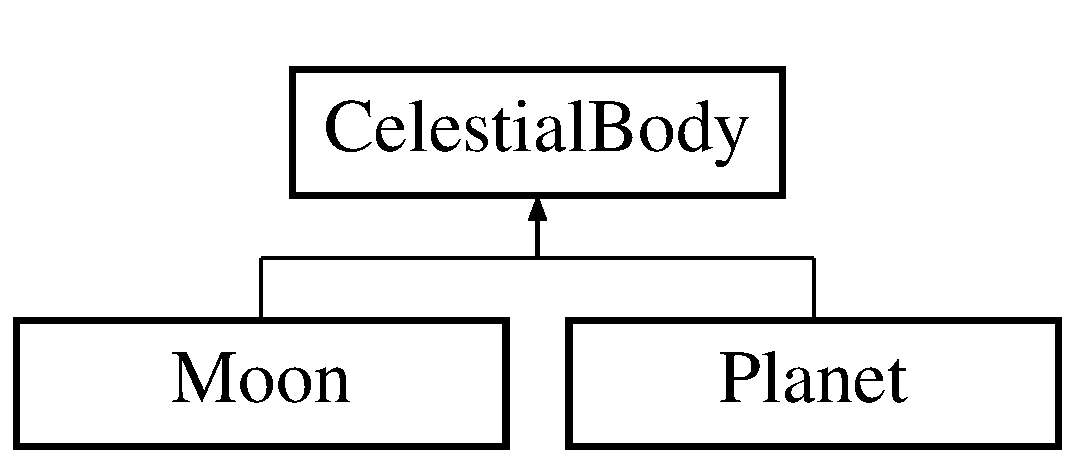
\includegraphics[height=2cm]{d4/d0b/classCelestialBody}
\end{center}
\end{figure}
\subsection*{Public Member Functions}
\begin{DoxyCompactItemize}
\item 
\hypertarget{classCelestialBody_adc6fec6a37c5ca24cd3c960e234d459b}{
virtual string {\bfseries getName} ()=0}
\label{d4/d0b/classCelestialBody_adc6fec6a37c5ca24cd3c960e234d459b}

\item 
\hypertarget{classCelestialBody_a0d582688d7873dd1ab37deea6d9e6f75}{
virtual int {\bfseries getTrianium} ()=0}
\label{d4/d0b/classCelestialBody_a0d582688d7873dd1ab37deea6d9e6f75}

\item 
\hypertarget{classCelestialBody_a91905e3d314dcb8546fefe5afe608ecf}{
virtual int {\bfseries getDilithium} ()=0}
\label{d4/d0b/classCelestialBody_a91905e3d314dcb8546fefe5afe608ecf}

\item 
\hypertarget{classCelestialBody_a9fb597600b74df80c8db04db4245b51f}{
virtual int {\bfseries getFood} ()=0}
\label{d4/d0b/classCelestialBody_a9fb597600b74df80c8db04db4245b51f}

\item 
\hypertarget{classCelestialBody_adf2ba9c0831a125d023513cc25639142}{
virtual int {\bfseries getWater} ()=0}
\label{d4/d0b/classCelestialBody_adf2ba9c0831a125d023513cc25639142}

\item 
\hypertarget{classCelestialBody_aae61fa7b39d4c23d1b831058bac186a0}{
virtual int {\bfseries getHealth} ()=0}
\label{d4/d0b/classCelestialBody_aae61fa7b39d4c23d1b831058bac186a0}

\item 
\hypertarget{classCelestialBody_a702fdc8427e6823fae9f3b10e77e59a7}{
virtual int {\bfseries getAthmosphericInterference} ()=0}
\label{d4/d0b/classCelestialBody_a702fdc8427e6823fae9f3b10e77e59a7}

\item 
\hypertarget{classCelestialBody_a19a84a9719569f12f74cc44174e27b67}{
virtual int {\bfseries getPlasma} ()=0}
\label{d4/d0b/classCelestialBody_a19a84a9719569f12f74cc44174e27b67}

\item 
\hypertarget{classCelestialBody_ab6797f9d41fefe5c77c7e08b32ec6787}{
virtual void {\bfseries setTrianium} (int val)=0}
\label{d4/d0b/classCelestialBody_ab6797f9d41fefe5c77c7e08b32ec6787}

\item 
\hypertarget{classCelestialBody_a8cd8dbd4e5a4d3caba0027d53a793495}{
virtual void {\bfseries setDilithium} (int val)=0}
\label{d4/d0b/classCelestialBody_a8cd8dbd4e5a4d3caba0027d53a793495}

\item 
\hypertarget{classCelestialBody_a8e56861f9b6e875aa48f15f37caeabc2}{
virtual void {\bfseries setFood} (int val)=0}
\label{d4/d0b/classCelestialBody_a8e56861f9b6e875aa48f15f37caeabc2}

\item 
\hypertarget{classCelestialBody_a762065cd0a5690bc94107b6a90bab584}{
virtual void {\bfseries setWater} (int val)=0}
\label{d4/d0b/classCelestialBody_a762065cd0a5690bc94107b6a90bab584}

\item 
\hypertarget{classCelestialBody_ab45bbf0a8775c538e2a0ee21b67fdac9}{
virtual void {\bfseries setHealth} (int val)=0}
\label{d4/d0b/classCelestialBody_ab45bbf0a8775c538e2a0ee21b67fdac9}

\item 
\hypertarget{classCelestialBody_a5b74f1050aeb75f9031e965c491c884d}{
virtual void {\bfseries setAthmosphericInterference} (int val)=0}
\label{d4/d0b/classCelestialBody_a5b74f1050aeb75f9031e965c491c884d}

\item 
\hypertarget{classCelestialBody_ab5806c7f2a6f1feeeaceb88eb5685ab0}{
virtual void {\bfseries setPlasma} (int val)=0}
\label{d4/d0b/classCelestialBody_ab5806c7f2a6f1feeeaceb88eb5685ab0}

\item 
\hypertarget{classCelestialBody_af729a04451951829bf586148f1c29d95}{
virtual bool {\bfseries getGas} ()=0}
\label{d4/d0b/classCelestialBody_af729a04451951829bf586148f1c29d95}

\item 
virtual vector$<$ \hyperlink{classCelestialBody}{CelestialBody} $\ast$ $>$ \hyperlink{classCelestialBody_a6c9db5c520596bc85a2e2a461db4b2c8}{getMoons} ()
\item 
virtual int \hyperlink{classCelestialBody_ae41a354c4b3345c7558c9691bc7c239e}{getNumMoons} ()
\item 
virtual void \hyperlink{classCelestialBody_a6e7b86fa71d74ad29e2434c4715b5608}{scanMoon} (unsigned int i)
\item 
virtual \hyperlink{classCelestialBody}{CelestialBody} $\ast$ \hyperlink{classCelestialBody_a7919f1dba305a225978fa901a34daf25}{targetMoon} (unsigned int i)
\end{DoxyCompactItemize}
\subsection*{Protected Attributes}
\begin{DoxyCompactItemize}
\item 
\hypertarget{classCelestialBody_a2feb5c10ef03fbe9491cb9b5cc33892f}{
string {\bfseries name}}
\label{d4/d0b/classCelestialBody_a2feb5c10ef03fbe9491cb9b5cc33892f}

\item 
\hypertarget{classCelestialBody_ae8c5da8051d418f78376a8a3d5ea4c47}{
int {\bfseries trianium}}
\label{d4/d0b/classCelestialBody_ae8c5da8051d418f78376a8a3d5ea4c47}

\item 
\hypertarget{classCelestialBody_af37a320affe85527f97581dae06189e8}{
int {\bfseries dilithium}}
\label{d4/d0b/classCelestialBody_af37a320affe85527f97581dae06189e8}

\item 
\hypertarget{classCelestialBody_acb0433e627eb4d204b0646157e247b94}{
int {\bfseries foodSupply}}
\label{d4/d0b/classCelestialBody_acb0433e627eb4d204b0646157e247b94}

\item 
\hypertarget{classCelestialBody_a90a3e2f3a52854a126cab26c32730d72}{
int {\bfseries waterSupply}}
\label{d4/d0b/classCelestialBody_a90a3e2f3a52854a126cab26c32730d72}

\item 
\hypertarget{classCelestialBody_aaeb14d0b014a7ddfde1bb15d92401085}{
int {\bfseries health}}
\label{d4/d0b/classCelestialBody_aaeb14d0b014a7ddfde1bb15d92401085}

\item 
\hypertarget{classCelestialBody_ab34e28203a9d135b3c3215d533af43a0}{
int {\bfseries athmosphericInterference}}
\label{d4/d0b/classCelestialBody_ab34e28203a9d135b3c3215d533af43a0}

\item 
\hypertarget{classCelestialBody_ad3153751e1714cc2bff3c5e624419eeb}{
int {\bfseries plasma}}
\label{d4/d0b/classCelestialBody_ad3153751e1714cc2bff3c5e624419eeb}

\item 
\hypertarget{classCelestialBody_af3b8f214ebaf09314fe723143e4b14f9}{
bool {\bfseries gasGiant}}
\label{d4/d0b/classCelestialBody_af3b8f214ebaf09314fe723143e4b14f9}

\item 
\hypertarget{classCelestialBody_a83e149bb1da99a9ee406d23ab6742812}{
vector$<$ \hyperlink{classCelestialBody}{CelestialBody} $\ast$ $>$ {\bfseries moons}}
\label{d4/d0b/classCelestialBody_a83e149bb1da99a9ee406d23ab6742812}

\item 
\hypertarget{classCelestialBody_aaccb8752c02fb47718d76343d34d8225}{
int {\bfseries numMoons}}
\label{d4/d0b/classCelestialBody_aaccb8752c02fb47718d76343d34d8225}

\end{DoxyCompactItemize}


\subsection{Member Function Documentation}
\hypertarget{classCelestialBody_a6c9db5c520596bc85a2e2a461db4b2c8}{
\index{CelestialBody@{CelestialBody}!getMoons@{getMoons}}
\index{getMoons@{getMoons}!CelestialBody@{CelestialBody}}
\subsubsection[{getMoons}]{\setlength{\rightskip}{0pt plus 5cm}vector$<$ {\bf CelestialBody} $\ast$ $>$ CelestialBody::getMoons ()\hspace{0.3cm}{\ttfamily  \mbox{[}virtual\mbox{]}}}}
\label{d4/d0b/classCelestialBody_a6c9db5c520596bc85a2e2a461db4b2c8}
To be overridden by the sub class returns a copy of the moons vector

\begin{DoxyReturn}{Returns}
vector$<$CelestialBody$\ast$$>$ 
\end{DoxyReturn}


Reimplemented in \hyperlink{classPlanet_ac003f70ce4149dc5d87423dace7de0b1}{Planet}.

\hypertarget{classCelestialBody_ae41a354c4b3345c7558c9691bc7c239e}{
\index{CelestialBody@{CelestialBody}!getNumMoons@{getNumMoons}}
\index{getNumMoons@{getNumMoons}!CelestialBody@{CelestialBody}}
\subsubsection[{getNumMoons}]{\setlength{\rightskip}{0pt plus 5cm}int CelestialBody::getNumMoons ()\hspace{0.3cm}{\ttfamily  \mbox{[}virtual\mbox{]}}}}
\label{d4/d0b/classCelestialBody_ae41a354c4b3345c7558c9691bc7c239e}
To be overridden by the sub class gets the amount of celestialbody moons

\begin{DoxyReturn}{Returns}
int number of moons 
\end{DoxyReturn}


Reimplemented in \hyperlink{classPlanet_a4c5cc040f92ec9fde52a4cccd04b69ff}{Planet}.

\hypertarget{classCelestialBody_a6e7b86fa71d74ad29e2434c4715b5608}{
\index{CelestialBody@{CelestialBody}!scanMoon@{scanMoon}}
\index{scanMoon@{scanMoon}!CelestialBody@{CelestialBody}}
\subsubsection[{scanMoon}]{\setlength{\rightskip}{0pt plus 5cm}void CelestialBody::scanMoon (unsigned int {\em i})\hspace{0.3cm}{\ttfamily  \mbox{[}virtual\mbox{]}}}}
\label{d4/d0b/classCelestialBody_a6e7b86fa71d74ad29e2434c4715b5608}
To be overridden by the sub class scans a celestialbody (moon) in he vector


\begin{DoxyParams}{Parameters}
\item[{\em i}]the moon index in the vector\end{DoxyParams}
\begin{DoxyReturn}{Returns}
void 
\end{DoxyReturn}


Reimplemented in \hyperlink{classPlanet_ad039e19380947fbf2695d78d4059f1db}{Planet}.

\hypertarget{classCelestialBody_a7919f1dba305a225978fa901a34daf25}{
\index{CelestialBody@{CelestialBody}!targetMoon@{targetMoon}}
\index{targetMoon@{targetMoon}!CelestialBody@{CelestialBody}}
\subsubsection[{targetMoon}]{\setlength{\rightskip}{0pt plus 5cm}{\bf CelestialBody} $\ast$ CelestialBody::targetMoon (unsigned int {\em i})\hspace{0.3cm}{\ttfamily  \mbox{[}virtual\mbox{]}}}}
\label{d4/d0b/classCelestialBody_a7919f1dba305a225978fa901a34daf25}
To be overridden by the sub class gets a pointer to a moon


\begin{DoxyParams}{Parameters}
\item[{\em i}]the index in the moons vector\end{DoxyParams}
\begin{DoxyReturn}{Returns}
CelestialBody$\ast$ a pointer to a moon 
\end{DoxyReturn}


Reimplemented in \hyperlink{classPlanet_a86eb8c5701ace894c2ca47b80ae776e9}{Planet}.



The documentation for this class was generated from the following files:\begin{DoxyCompactItemize}
\item 
source/header/CelestialBody.h\item 
source/source/CelestialBody.cpp\end{DoxyCompactItemize}

\hypertarget{structcell__t}{
\section{cell\_\-t Struct Reference}
\label{d9/d8a/structcell__t}\index{cell\_\-t@{cell\_\-t}}
}
\subsection*{Public Attributes}
\begin{DoxyCompactItemize}
\item 
\hypertarget{structcell__t_aca4a99c0cb9afa972a7d0b21211a03ab}{
unsigned int {\bfseries up}: 1}
\label{d9/d8a/structcell__t_aca4a99c0cb9afa972a7d0b21211a03ab}

\item 
\hypertarget{structcell__t_a4316cad340f54a20c1551742054ce38f}{
unsigned int {\bfseries right}: 1}
\label{d9/d8a/structcell__t_a4316cad340f54a20c1551742054ce38f}

\item 
\hypertarget{structcell__t_a3e0b733a05da0b1181e4a433670f8a81}{
unsigned int {\bfseries down}: 1}
\label{d9/d8a/structcell__t_a3e0b733a05da0b1181e4a433670f8a81}

\item 
\hypertarget{structcell__t_adce82b9aef49dbafa817eabc4541769c}{
unsigned int {\bfseries left}: 1}
\label{d9/d8a/structcell__t_adce82b9aef49dbafa817eabc4541769c}

\item 
\hypertarget{structcell__t_a87ea82717113f9ea45077a11fbb3f5c5}{
unsigned int {\bfseries path}: 1}
\label{d9/d8a/structcell__t_a87ea82717113f9ea45077a11fbb3f5c5}

\item 
\hypertarget{structcell__t_a4efaf27751f0ecc83a49c3cb1a17e1f1}{
unsigned int {\bfseries visited}: 1}
\label{d9/d8a/structcell__t_a4efaf27751f0ecc83a49c3cb1a17e1f1}

\end{DoxyCompactItemize}


The documentation for this struct was generated from the following file:\begin{DoxyCompactItemize}
\item 
source/header/Maze.h\end{DoxyCompactItemize}

\hypertarget{classCommand}{
\section{Command Class Reference}
\label{d9/d71/classCommand}\index{Command@{Command}}
}
\subsection*{Public Member Functions}
\begin{DoxyCompactItemize}
\item 
\hyperlink{classCommand_a42ecf6585cb454ebb1c7422993c636b3}{Command} (string firstWord, string secondWord, string thirdWord)
\item 
\hyperlink{classCommand_ab552bb3a07fdd1acbfd8ea76e69b2278}{$\sim$Command} ()
\item 
string \hyperlink{classCommand_a03a9986a1e2adc85ef1aaf02a3387216}{getCommandWord} ()
\item 
string \hyperlink{classCommand_a977ac7e151122d5174d74f8663725ea0}{getSecondWord} ()
\item 
string \hyperlink{classCommand_adb921b62cb34feb6dd522e7b9c4f23dd}{getThirdWord} ()
\item 
bool \hyperlink{classCommand_a15fba440e0eb3df75bea367448f52a1a}{isUnknown} ()
\item 
bool \hyperlink{classCommand_a6a71c6f60df54f00671fd993a267d6fc}{hasSecondWord} ()
\item 
bool \hyperlink{classCommand_a6c94c33f7e5fae0a4ce604bf998603e6}{hasThirdWord} ()
\end{DoxyCompactItemize}


\subsection{Constructor \& Destructor Documentation}
\hypertarget{classCommand_a42ecf6585cb454ebb1c7422993c636b3}{
\index{Command@{Command}!Command@{Command}}
\index{Command@{Command}!Command@{Command}}
\subsubsection[{Command}]{\setlength{\rightskip}{0pt plus 5cm}Command::Command (string {\em firstWord}, \/  string {\em secondWord}, \/  string {\em thirdWord})}}
\label{d9/d71/classCommand_a42ecf6585cb454ebb1c7422993c636b3}
Constructor 
\begin{DoxyParams}{Parameters}
\item[{\em firstWord}](command word) \item[{\em secondWord}]\item[{\em thirdWord}]\end{DoxyParams}
\hypertarget{classCommand_ab552bb3a07fdd1acbfd8ea76e69b2278}{
\index{Command@{Command}!$\sim$Command@{$\sim$Command}}
\index{$\sim$Command@{$\sim$Command}!Command@{Command}}
\subsubsection[{$\sim$Command}]{\setlength{\rightskip}{0pt plus 5cm}Command::$\sim$Command ()}}
\label{d9/d71/classCommand_ab552bb3a07fdd1acbfd8ea76e69b2278}
Destructor for the command word object 

\subsection{Member Function Documentation}
\hypertarget{classCommand_a03a9986a1e2adc85ef1aaf02a3387216}{
\index{Command@{Command}!getCommandWord@{getCommandWord}}
\index{getCommandWord@{getCommandWord}!Command@{Command}}
\subsubsection[{getCommandWord}]{\setlength{\rightskip}{0pt plus 5cm}string Command::getCommandWord ()}}
\label{d9/d71/classCommand_a03a9986a1e2adc85ef1aaf02a3387216}
returns the command word of the command

\begin{DoxyReturn}{Returns}
string 
\end{DoxyReturn}
\hypertarget{classCommand_a977ac7e151122d5174d74f8663725ea0}{
\index{Command@{Command}!getSecondWord@{getSecondWord}}
\index{getSecondWord@{getSecondWord}!Command@{Command}}
\subsubsection[{getSecondWord}]{\setlength{\rightskip}{0pt plus 5cm}string Command::getSecondWord ()}}
\label{d9/d71/classCommand_a977ac7e151122d5174d74f8663725ea0}
returns the second word of the command

\begin{DoxyReturn}{Returns}
string 
\end{DoxyReturn}
\hypertarget{classCommand_adb921b62cb34feb6dd522e7b9c4f23dd}{
\index{Command@{Command}!getThirdWord@{getThirdWord}}
\index{getThirdWord@{getThirdWord}!Command@{Command}}
\subsubsection[{getThirdWord}]{\setlength{\rightskip}{0pt plus 5cm}string Command::getThirdWord ()}}
\label{d9/d71/classCommand_adb921b62cb34feb6dd522e7b9c4f23dd}
returns the third word of the command

\begin{DoxyReturn}{Returns}
string 
\end{DoxyReturn}
\hypertarget{classCommand_a6a71c6f60df54f00671fd993a267d6fc}{
\index{Command@{Command}!hasSecondWord@{hasSecondWord}}
\index{hasSecondWord@{hasSecondWord}!Command@{Command}}
\subsubsection[{hasSecondWord}]{\setlength{\rightskip}{0pt plus 5cm}bool Command::hasSecondWord ()}}
\label{d9/d71/classCommand_a6a71c6f60df54f00671fd993a267d6fc}
returns true of the command has a second word

\begin{DoxyReturn}{Returns}
bool 
\end{DoxyReturn}
\hypertarget{classCommand_a6c94c33f7e5fae0a4ce604bf998603e6}{
\index{Command@{Command}!hasThirdWord@{hasThirdWord}}
\index{hasThirdWord@{hasThirdWord}!Command@{Command}}
\subsubsection[{hasThirdWord}]{\setlength{\rightskip}{0pt plus 5cm}bool Command::hasThirdWord ()}}
\label{d9/d71/classCommand_a6c94c33f7e5fae0a4ce604bf998603e6}
returns true of the command has a third word

\begin{DoxyReturn}{Returns}
bool 
\end{DoxyReturn}
\hypertarget{classCommand_a15fba440e0eb3df75bea367448f52a1a}{
\index{Command@{Command}!isUnknown@{isUnknown}}
\index{isUnknown@{isUnknown}!Command@{Command}}
\subsubsection[{isUnknown}]{\setlength{\rightskip}{0pt plus 5cm}bool Command::isUnknown ()}}
\label{d9/d71/classCommand_a15fba440e0eb3df75bea367448f52a1a}
returns true i the command word exists in the vector

\begin{DoxyReturn}{Returns}
bool 
\end{DoxyReturn}


The documentation for this class was generated from the following files:\begin{DoxyCompactItemize}
\item 
source/header/Command.h\item 
source/source/Command.cpp\end{DoxyCompactItemize}

\hypertarget{classCommandWords}{
\section{CommandWords Class Reference}
\label{d0/dda/classCommandWords}\index{CommandWords@{CommandWords}}
}
\subsection*{Public Member Functions}
\begin{DoxyCompactItemize}
\item 
\hyperlink{classCommandWords_a778ed5312468a58785c55e4df67fe8c2}{CommandWords} ()
\item 
\hyperlink{classCommandWords_a9802c2d1589170dde629f70015848253}{$\sim$CommandWords} ()
\item 
bool \hyperlink{classCommandWords_a462e98022a37c1699c14d45ab59c3f3f}{isCommand} (string aString)
\item 
void \hyperlink{classCommandWords_aa449001a267676b74f1aacd89a6f84a4}{showAll} ()
\end{DoxyCompactItemize}


\subsection{Constructor \& Destructor Documentation}
\hypertarget{classCommandWords_a778ed5312468a58785c55e4df67fe8c2}{
\index{CommandWords@{CommandWords}!CommandWords@{CommandWords}}
\index{CommandWords@{CommandWords}!CommandWords@{CommandWords}}
\subsubsection[{CommandWords}]{\setlength{\rightskip}{0pt plus 5cm}CommandWords::CommandWords ()}}
\label{d0/dda/classCommandWords_a778ed5312468a58785c55e4df67fe8c2}
Constructor adds valid commands and descriptions to the vectors \hypertarget{classCommandWords_a9802c2d1589170dde629f70015848253}{
\index{CommandWords@{CommandWords}!$\sim$CommandWords@{$\sim$CommandWords}}
\index{$\sim$CommandWords@{$\sim$CommandWords}!CommandWords@{CommandWords}}
\subsubsection[{$\sim$CommandWords}]{\setlength{\rightskip}{0pt plus 5cm}CommandWords::$\sim$CommandWords ()}}
\label{d0/dda/classCommandWords_a9802c2d1589170dde629f70015848253}
Destructor for commands 

\subsection{Member Function Documentation}
\hypertarget{classCommandWords_a462e98022a37c1699c14d45ab59c3f3f}{
\index{CommandWords@{CommandWords}!isCommand@{isCommand}}
\index{isCommand@{isCommand}!CommandWords@{CommandWords}}
\subsubsection[{isCommand}]{\setlength{\rightskip}{0pt plus 5cm}bool CommandWords::isCommand (string {\em aString})}}
\label{d0/dda/classCommandWords_a462e98022a37c1699c14d45ab59c3f3f}
Returns true if it is a valid command


\begin{DoxyParams}{Parameters}
\item[{\em aString}]the command word to test against the valid commands\end{DoxyParams}
\begin{DoxyReturn}{Returns}
bool is valid command 
\end{DoxyReturn}
\hypertarget{classCommandWords_aa449001a267676b74f1aacd89a6f84a4}{
\index{CommandWords@{CommandWords}!showAll@{showAll}}
\index{showAll@{showAll}!CommandWords@{CommandWords}}
\subsubsection[{showAll}]{\setlength{\rightskip}{0pt plus 5cm}void CommandWords::showAll ()}}
\label{d0/dda/classCommandWords_aa449001a267676b74f1aacd89a6f84a4}
Shows all the commands and their descriptions to the user

\begin{DoxyReturn}{Returns}
void 
\end{DoxyReturn}


The documentation for this class was generated from the following files:\begin{DoxyCompactItemize}
\item 
source/header/CommandWords.h\item 
source/source/CommandWords.cpp\end{DoxyCompactItemize}

\hypertarget{classMoon}{
\section{Moon Class Reference}
\label{d8/d6f/classMoon}\index{Moon@{Moon}}
}
Inheritance diagram for Moon:\begin{figure}[H]
\begin{center}
\leavevmode
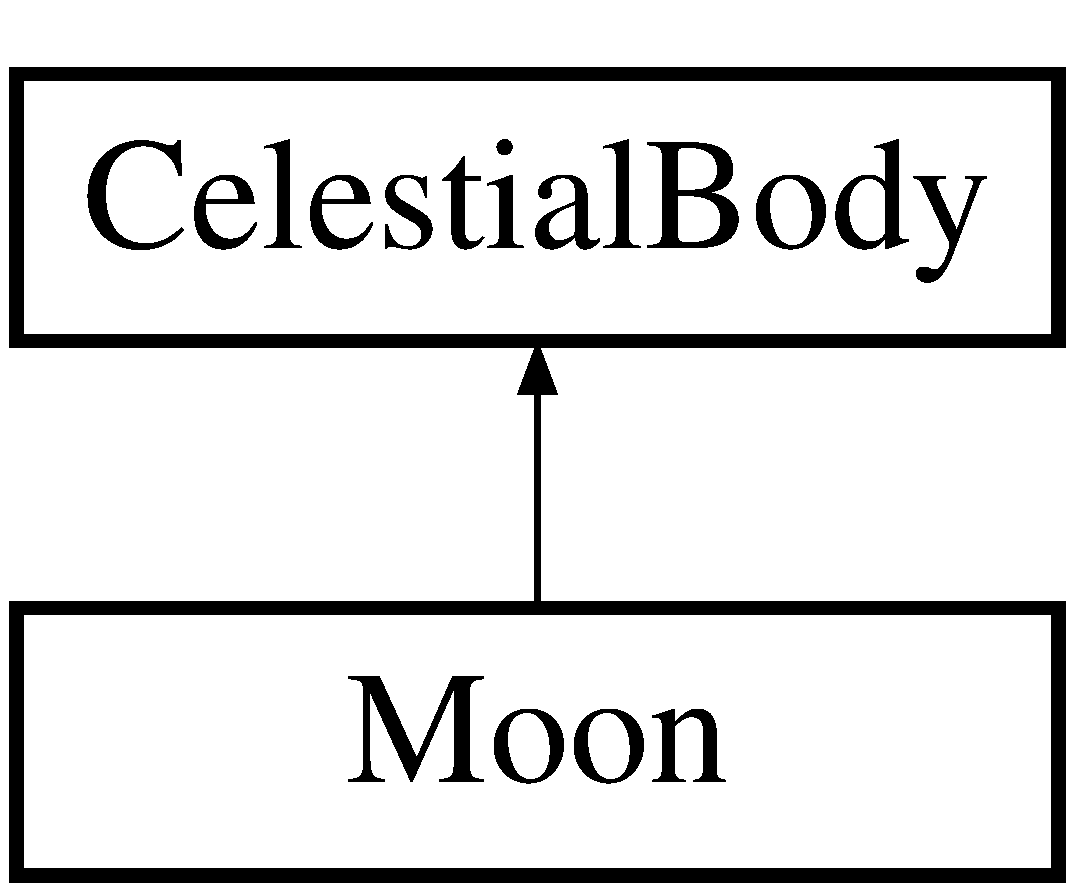
\includegraphics[height=2cm]{d8/d6f/classMoon}
\end{center}
\end{figure}
\subsection*{Public Member Functions}
\begin{DoxyCompactItemize}
\item 
\hyperlink{classMoon_a5215a61100839fba014a10816182c601}{Moon} (string name)
\item 
string \hyperlink{classMoon_a7015a95bbb104f0fc3b46ece7a427655}{getName} ()
\item 
int \hyperlink{classMoon_afa9d20396dcd4a5501fe1ee9c0a23397}{getTrianium} ()
\item 
int \hyperlink{classMoon_ac79186e5684da6bebfd9821ff655bc71}{getDilithium} ()
\item 
int \hyperlink{classMoon_a790c4ae16bde7df44f608c98a535afec}{getFood} ()
\item 
int \hyperlink{classMoon_a6d687ec0a5f6437b0af4615241afe94f}{getWater} ()
\item 
int \hyperlink{classMoon_a70626fe26dfa798f21791cc182a829f4}{getHealth} ()
\item 
int \hyperlink{classMoon_af15b50721bac099545c7a0be97d04483}{getAthmosphericInterference} ()
\item 
int \hyperlink{classMoon_acc0fef605a7fd18d16aff7e827e9bf9a}{getPlasma} ()
\item 
void \hyperlink{classMoon_a76c433c77c0efca8fd093630b1767f13}{setTrianium} (int val)
\item 
void \hyperlink{classMoon_ab73d920601c3f398cb23b2d78f816f49}{setDilithium} (int val)
\item 
void \hyperlink{classMoon_a525d52c5f9c8582d2e81dfc30f97dd1c}{setFood} (int val)
\item 
void \hyperlink{classMoon_a489d140b5ff38114cd0f5f15512a99d4}{setWater} (int val)
\item 
void \hyperlink{classMoon_ae6ba20c5d4f9b6ac33d35d2e31452089}{setHealth} (int val)
\item 
void \hyperlink{classMoon_a1088a8f3e7198b38d9ce498f9f6243a9}{setAthmosphericInterference} (int val)
\item 
void \hyperlink{classMoon_a3bff2a5c897c5c66b6e16b16077ba1cc}{setPlasma} (int val)
\item 
bool \hyperlink{classMoon_ad7881084092664bd2bd72a12552fb4a0}{getGas} ()
\end{DoxyCompactItemize}


\subsection{Constructor \& Destructor Documentation}
\hypertarget{classMoon_a5215a61100839fba014a10816182c601}{
\index{Moon@{Moon}!Moon@{Moon}}
\index{Moon@{Moon}!Moon@{Moon}}
\subsubsection[{Moon}]{\setlength{\rightskip}{0pt plus 5cm}Moon::Moon (string {\em name})}}
\label{d8/d6f/classMoon_a5215a61100839fba014a10816182c601}
Constructor


\begin{DoxyParams}{Parameters}
\item[{\em string}]the name of the moon \end{DoxyParams}


\subsection{Member Function Documentation}
\hypertarget{classMoon_af15b50721bac099545c7a0be97d04483}{
\index{Moon@{Moon}!getAthmosphericInterference@{getAthmosphericInterference}}
\index{getAthmosphericInterference@{getAthmosphericInterference}!Moon@{Moon}}
\subsubsection[{getAthmosphericInterference}]{\setlength{\rightskip}{0pt plus 5cm}int Moon::getAthmosphericInterference ()\hspace{0.3cm}{\ttfamily  \mbox{[}virtual\mbox{]}}}}
\label{d8/d6f/classMoon_af15b50721bac099545c7a0be97d04483}
Accessor for the celestial body data member athmospheric interferance

\begin{DoxyReturn}{Returns}
int 
\end{DoxyReturn}


Implements \hyperlink{classCelestialBody}{CelestialBody}.

\hypertarget{classMoon_ac79186e5684da6bebfd9821ff655bc71}{
\index{Moon@{Moon}!getDilithium@{getDilithium}}
\index{getDilithium@{getDilithium}!Moon@{Moon}}
\subsubsection[{getDilithium}]{\setlength{\rightskip}{0pt plus 5cm}int Moon::getDilithium ()\hspace{0.3cm}{\ttfamily  \mbox{[}virtual\mbox{]}}}}
\label{d8/d6f/classMoon_ac79186e5684da6bebfd9821ff655bc71}
Accessor for the celestial body data member dilthium

\begin{DoxyReturn}{Returns}
int 
\end{DoxyReturn}


Implements \hyperlink{classCelestialBody}{CelestialBody}.

\hypertarget{classMoon_a790c4ae16bde7df44f608c98a535afec}{
\index{Moon@{Moon}!getFood@{getFood}}
\index{getFood@{getFood}!Moon@{Moon}}
\subsubsection[{getFood}]{\setlength{\rightskip}{0pt plus 5cm}int Moon::getFood ()\hspace{0.3cm}{\ttfamily  \mbox{[}virtual\mbox{]}}}}
\label{d8/d6f/classMoon_a790c4ae16bde7df44f608c98a535afec}
Accessor for the celestial body data member food

\begin{DoxyReturn}{Returns}
int 
\end{DoxyReturn}


Implements \hyperlink{classCelestialBody}{CelestialBody}.

\hypertarget{classMoon_ad7881084092664bd2bd72a12552fb4a0}{
\index{Moon@{Moon}!getGas@{getGas}}
\index{getGas@{getGas}!Moon@{Moon}}
\subsubsection[{getGas}]{\setlength{\rightskip}{0pt plus 5cm}bool Moon::getGas ()\hspace{0.3cm}{\ttfamily  \mbox{[}virtual\mbox{]}}}}
\label{d8/d6f/classMoon_ad7881084092664bd2bd72a12552fb4a0}
Accessor for the celestial body data member gasgiant

\begin{DoxyReturn}{Returns}
int 
\end{DoxyReturn}


Implements \hyperlink{classCelestialBody}{CelestialBody}.

\hypertarget{classMoon_a70626fe26dfa798f21791cc182a829f4}{
\index{Moon@{Moon}!getHealth@{getHealth}}
\index{getHealth@{getHealth}!Moon@{Moon}}
\subsubsection[{getHealth}]{\setlength{\rightskip}{0pt plus 5cm}int Moon::getHealth ()\hspace{0.3cm}{\ttfamily  \mbox{[}virtual\mbox{]}}}}
\label{d8/d6f/classMoon_a70626fe26dfa798f21791cc182a829f4}
Accessor for the celestial body data member health

\begin{DoxyReturn}{Returns}
int 
\end{DoxyReturn}


Implements \hyperlink{classCelestialBody}{CelestialBody}.

\hypertarget{classMoon_a7015a95bbb104f0fc3b46ece7a427655}{
\index{Moon@{Moon}!getName@{getName}}
\index{getName@{getName}!Moon@{Moon}}
\subsubsection[{getName}]{\setlength{\rightskip}{0pt plus 5cm}string Moon::getName ()\hspace{0.3cm}{\ttfamily  \mbox{[}virtual\mbox{]}}}}
\label{d8/d6f/classMoon_a7015a95bbb104f0fc3b46ece7a427655}
Returns the name of this CelestialObject (moon)

\begin{DoxyReturn}{Returns}
string 
\end{DoxyReturn}


Implements \hyperlink{classCelestialBody}{CelestialBody}.

\hypertarget{classMoon_acc0fef605a7fd18d16aff7e827e9bf9a}{
\index{Moon@{Moon}!getPlasma@{getPlasma}}
\index{getPlasma@{getPlasma}!Moon@{Moon}}
\subsubsection[{getPlasma}]{\setlength{\rightskip}{0pt plus 5cm}int Moon::getPlasma ()\hspace{0.3cm}{\ttfamily  \mbox{[}virtual\mbox{]}}}}
\label{d8/d6f/classMoon_acc0fef605a7fd18d16aff7e827e9bf9a}
Accessor for the celestial body data member plasma

\begin{DoxyReturn}{Returns}
int 
\end{DoxyReturn}


Implements \hyperlink{classCelestialBody}{CelestialBody}.

\hypertarget{classMoon_afa9d20396dcd4a5501fe1ee9c0a23397}{
\index{Moon@{Moon}!getTrianium@{getTrianium}}
\index{getTrianium@{getTrianium}!Moon@{Moon}}
\subsubsection[{getTrianium}]{\setlength{\rightskip}{0pt plus 5cm}int Moon::getTrianium ()\hspace{0.3cm}{\ttfamily  \mbox{[}virtual\mbox{]}}}}
\label{d8/d6f/classMoon_afa9d20396dcd4a5501fe1ee9c0a23397}
Accessor for the celestial body data member trianium

\begin{DoxyReturn}{Returns}
int 
\end{DoxyReturn}


Implements \hyperlink{classCelestialBody}{CelestialBody}.

\hypertarget{classMoon_a6d687ec0a5f6437b0af4615241afe94f}{
\index{Moon@{Moon}!getWater@{getWater}}
\index{getWater@{getWater}!Moon@{Moon}}
\subsubsection[{getWater}]{\setlength{\rightskip}{0pt plus 5cm}int Moon::getWater ()\hspace{0.3cm}{\ttfamily  \mbox{[}virtual\mbox{]}}}}
\label{d8/d6f/classMoon_a6d687ec0a5f6437b0af4615241afe94f}
Accessor for the celestial body data member water

\begin{DoxyReturn}{Returns}
int 
\end{DoxyReturn}


Implements \hyperlink{classCelestialBody}{CelestialBody}.

\hypertarget{classMoon_a1088a8f3e7198b38d9ce498f9f6243a9}{
\index{Moon@{Moon}!setAthmosphericInterference@{setAthmosphericInterference}}
\index{setAthmosphericInterference@{setAthmosphericInterference}!Moon@{Moon}}
\subsubsection[{setAthmosphericInterference}]{\setlength{\rightskip}{0pt plus 5cm}void Moon::setAthmosphericInterference (int {\em val})\hspace{0.3cm}{\ttfamily  \mbox{[}virtual\mbox{]}}}}
\label{d8/d6f/classMoon_a1088a8f3e7198b38d9ce498f9f6243a9}
Mutator for the celestial body data member athmospheric interferance


\begin{DoxyParams}{Parameters}
\item[{\em int}]\end{DoxyParams}
\begin{DoxyReturn}{Returns}
void 
\end{DoxyReturn}


Implements \hyperlink{classCelestialBody}{CelestialBody}.

\hypertarget{classMoon_ab73d920601c3f398cb23b2d78f816f49}{
\index{Moon@{Moon}!setDilithium@{setDilithium}}
\index{setDilithium@{setDilithium}!Moon@{Moon}}
\subsubsection[{setDilithium}]{\setlength{\rightskip}{0pt plus 5cm}void Moon::setDilithium (int {\em val})\hspace{0.3cm}{\ttfamily  \mbox{[}virtual\mbox{]}}}}
\label{d8/d6f/classMoon_ab73d920601c3f398cb23b2d78f816f49}
Mutator for the celestial body data member dilithium


\begin{DoxyParams}{Parameters}
\item[{\em int}]\end{DoxyParams}
\begin{DoxyReturn}{Returns}
void 
\end{DoxyReturn}


Implements \hyperlink{classCelestialBody}{CelestialBody}.

\hypertarget{classMoon_a525d52c5f9c8582d2e81dfc30f97dd1c}{
\index{Moon@{Moon}!setFood@{setFood}}
\index{setFood@{setFood}!Moon@{Moon}}
\subsubsection[{setFood}]{\setlength{\rightskip}{0pt plus 5cm}void Moon::setFood (int {\em val})\hspace{0.3cm}{\ttfamily  \mbox{[}virtual\mbox{]}}}}
\label{d8/d6f/classMoon_a525d52c5f9c8582d2e81dfc30f97dd1c}
Mutator for the celestial body data member food


\begin{DoxyParams}{Parameters}
\item[{\em int}]\end{DoxyParams}
\begin{DoxyReturn}{Returns}
void 
\end{DoxyReturn}


Implements \hyperlink{classCelestialBody}{CelestialBody}.

\hypertarget{classMoon_ae6ba20c5d4f9b6ac33d35d2e31452089}{
\index{Moon@{Moon}!setHealth@{setHealth}}
\index{setHealth@{setHealth}!Moon@{Moon}}
\subsubsection[{setHealth}]{\setlength{\rightskip}{0pt plus 5cm}void Moon::setHealth (int {\em val})\hspace{0.3cm}{\ttfamily  \mbox{[}virtual\mbox{]}}}}
\label{d8/d6f/classMoon_ae6ba20c5d4f9b6ac33d35d2e31452089}
Mutator for the celestial body data member health


\begin{DoxyParams}{Parameters}
\item[{\em int}]\end{DoxyParams}
\begin{DoxyReturn}{Returns}
void 
\end{DoxyReturn}


Implements \hyperlink{classCelestialBody}{CelestialBody}.

\hypertarget{classMoon_a3bff2a5c897c5c66b6e16b16077ba1cc}{
\index{Moon@{Moon}!setPlasma@{setPlasma}}
\index{setPlasma@{setPlasma}!Moon@{Moon}}
\subsubsection[{setPlasma}]{\setlength{\rightskip}{0pt plus 5cm}void Moon::setPlasma (int {\em val})\hspace{0.3cm}{\ttfamily  \mbox{[}virtual\mbox{]}}}}
\label{d8/d6f/classMoon_a3bff2a5c897c5c66b6e16b16077ba1cc}
Mutator for the celestial body data member plasma


\begin{DoxyParams}{Parameters}
\item[{\em int}]\end{DoxyParams}
\begin{DoxyReturn}{Returns}
void 
\end{DoxyReturn}


Implements \hyperlink{classCelestialBody}{CelestialBody}.

\hypertarget{classMoon_a76c433c77c0efca8fd093630b1767f13}{
\index{Moon@{Moon}!setTrianium@{setTrianium}}
\index{setTrianium@{setTrianium}!Moon@{Moon}}
\subsubsection[{setTrianium}]{\setlength{\rightskip}{0pt plus 5cm}void Moon::setTrianium (int {\em val})\hspace{0.3cm}{\ttfamily  \mbox{[}virtual\mbox{]}}}}
\label{d8/d6f/classMoon_a76c433c77c0efca8fd093630b1767f13}
Mutator for the celestial body data member trianium


\begin{DoxyParams}{Parameters}
\item[{\em int}]\end{DoxyParams}
\begin{DoxyReturn}{Returns}
void 
\end{DoxyReturn}


Implements \hyperlink{classCelestialBody}{CelestialBody}.

\hypertarget{classMoon_a489d140b5ff38114cd0f5f15512a99d4}{
\index{Moon@{Moon}!setWater@{setWater}}
\index{setWater@{setWater}!Moon@{Moon}}
\subsubsection[{setWater}]{\setlength{\rightskip}{0pt plus 5cm}void Moon::setWater (int {\em val})\hspace{0.3cm}{\ttfamily  \mbox{[}virtual\mbox{]}}}}
\label{d8/d6f/classMoon_a489d140b5ff38114cd0f5f15512a99d4}
Mutator for the celestial body data member water


\begin{DoxyParams}{Parameters}
\item[{\em int}]\end{DoxyParams}
\begin{DoxyReturn}{Returns}
void 
\end{DoxyReturn}


Implements \hyperlink{classCelestialBody}{CelestialBody}.



The documentation for this class was generated from the following files:\begin{DoxyCompactItemize}
\item 
source/header/Moon.h\item 
source/source/Moon.cpp\end{DoxyCompactItemize}

\hypertarget{classParser}{
\section{Parser Class Reference}
\label{d0/d40/classParser}\index{Parser@{Parser}}
}
\subsection*{Public Member Functions}
\begin{DoxyCompactItemize}
\item 
\hyperlink{classParser_a12234f6cd36b61af4b50c94a179422c1}{Parser} ()
\item 
\hyperlink{classParser_a3e658b5917a93a3ef648050d060e3a93}{$\sim$Parser} ()
\item 
\hyperlink{classCommand}{Command} $\ast$ \hyperlink{classParser_a76b5f7778dd0272abee80ab848a43960}{getCommand} (string prefix)
\item 
void \hyperlink{classParser_ab893322079a7bc6e6b2153da7d9468bd}{showCommands} ()
\end{DoxyCompactItemize}


\subsection{Constructor \& Destructor Documentation}
\hypertarget{classParser_a12234f6cd36b61af4b50c94a179422c1}{
\index{Parser@{Parser}!Parser@{Parser}}
\index{Parser@{Parser}!Parser@{Parser}}
\subsubsection[{Parser}]{\setlength{\rightskip}{0pt plus 5cm}Parser::Parser ()}}
\label{d0/d40/classParser_a12234f6cd36b61af4b50c94a179422c1}
constructor \hypertarget{classParser_a3e658b5917a93a3ef648050d060e3a93}{
\index{Parser@{Parser}!$\sim$Parser@{$\sim$Parser}}
\index{$\sim$Parser@{$\sim$Parser}!Parser@{Parser}}
\subsubsection[{$\sim$Parser}]{\setlength{\rightskip}{0pt plus 5cm}Parser::$\sim$Parser ()}}
\label{d0/d40/classParser_a3e658b5917a93a3ef648050d060e3a93}
destructor cleans up commands 

\subsection{Member Function Documentation}
\hypertarget{classParser_a76b5f7778dd0272abee80ab848a43960}{
\index{Parser@{Parser}!getCommand@{getCommand}}
\index{getCommand@{getCommand}!Parser@{Parser}}
\subsubsection[{getCommand}]{\setlength{\rightskip}{0pt plus 5cm}{\bf Command} $\ast$ Parser::getCommand (string {\em prefix})}}
\label{d0/d40/classParser_a76b5f7778dd0272abee80ab848a43960}
Creates a new copy of command for use in the main loop


\begin{DoxyParams}{Parameters}
\item[{\em string}]prefix to be added to the line at the user input\end{DoxyParams}
\begin{DoxyReturn}{Returns}
command 
\end{DoxyReturn}
\hypertarget{classParser_ab893322079a7bc6e6b2153da7d9468bd}{
\index{Parser@{Parser}!showCommands@{showCommands}}
\index{showCommands@{showCommands}!Parser@{Parser}}
\subsubsection[{showCommands}]{\setlength{\rightskip}{0pt plus 5cm}void Parser::showCommands ()}}
\label{d0/d40/classParser_ab893322079a7bc6e6b2153da7d9468bd}
Shows all the commands

\begin{DoxyReturn}{Returns}
void 
\end{DoxyReturn}


The documentation for this class was generated from the following files:\begin{DoxyCompactItemize}
\item 
source/header/Parser.h\item 
source/source/Parser.cpp\end{DoxyCompactItemize}

\hypertarget{classPlanet}{
\section{Planet Class Reference}
\label{d5/dec/classPlanet}\index{Planet@{Planet}}
}
Inheritance diagram for Planet:\begin{figure}[H]
\begin{center}
\leavevmode
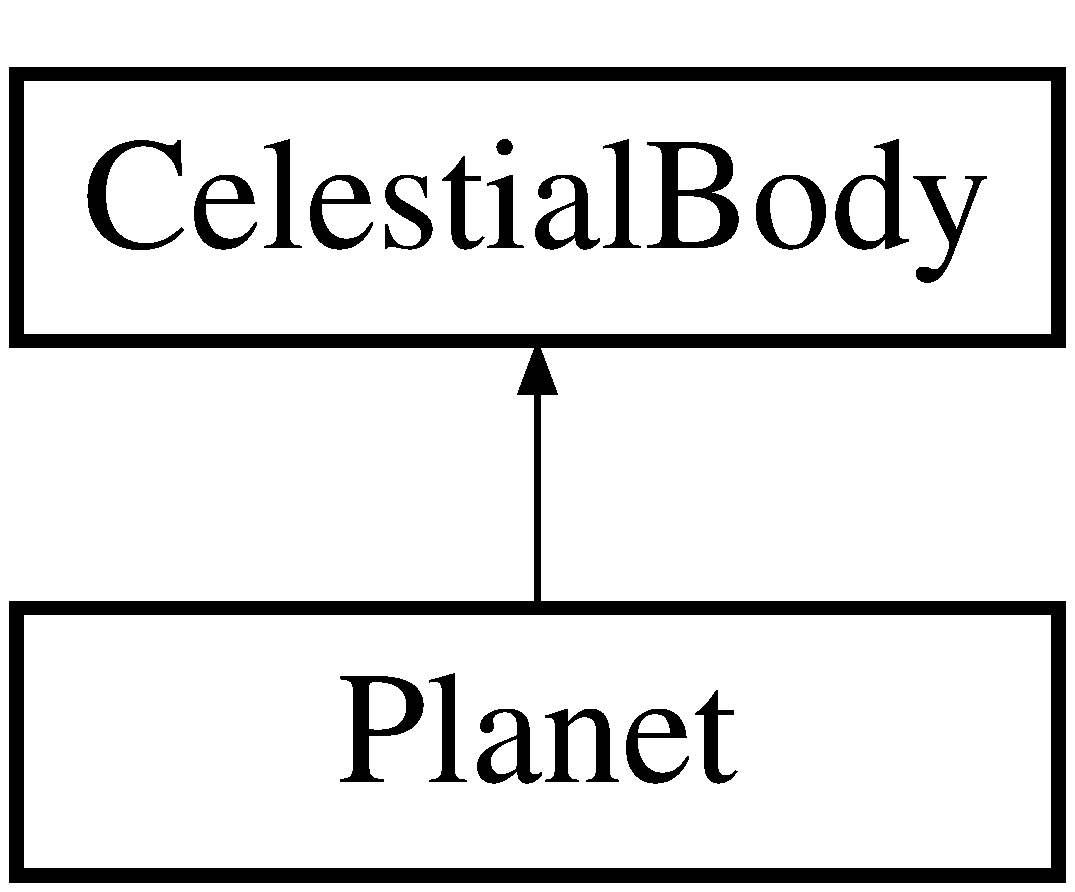
\includegraphics[height=2cm]{d5/dec/classPlanet}
\end{center}
\end{figure}
\subsection*{Public Member Functions}
\begin{DoxyCompactItemize}
\item 
\hyperlink{classPlanet_ac5a904c9d24bd4244ad72bb7ae3689f8}{Planet} (string name, \hyperlink{classStarTrekEntities}{StarTrekEntities} $\ast$stePointer)
\item 
\hyperlink{classPlanet_aaa1aaed9d4ef90b4836531edb7b18e0a}{$\sim$Planet} ()
\item 
string \hyperlink{classPlanet_a645b3d987a3001bac59a772b944607d2}{getName} ()
\item 
int \hyperlink{classPlanet_a37f64a787c17b5dd4471c8ad54fd9df0}{getTrianium} ()
\item 
int \hyperlink{classPlanet_a272240452921331e7220108df452a37d}{getDilithium} ()
\item 
int \hyperlink{classPlanet_a2b85fd628db9831d7ab5c7149b80cde3}{getFood} ()
\item 
int \hyperlink{classPlanet_af5bc4d184fcb72bd37f70119af5ecd89}{getWater} ()
\item 
int \hyperlink{classPlanet_a4499676225d09b0249cf225e795ce3cb}{getHealth} ()
\item 
int \hyperlink{classPlanet_a802c105bafd608a0ac57e8f03d2d2465}{getAthmosphericInterference} ()
\item 
int \hyperlink{classPlanet_ad7c07f51f9a447bf4aba45875e5f8e44}{getPlasma} ()
\item 
void \hyperlink{classPlanet_a298ae0e6344b5e83b4c53e5377b0531f}{setTrianium} (int val)
\item 
void \hyperlink{classPlanet_a780868e3c6275c2f8026bf7f7b910be1}{setDilithium} (int val)
\item 
void \hyperlink{classPlanet_a2f73c4ce9e4e4eb204b50413ea81d0cc}{setFood} (int val)
\item 
void \hyperlink{classPlanet_afbc0d813ae0d2a958487cfc2a06fd9d1}{setWater} (int val)
\item 
void \hyperlink{classPlanet_aa3ade00566dc836084395a25adc2cdb8}{setHealth} (int val)
\item 
void \hyperlink{classPlanet_a8f00e39da016ecdca4d1f0e7e8a76f5d}{setAthmosphericInterference} (int val)
\item 
void \hyperlink{classPlanet_a227e20f2716a12afddf50eddcd7c10c5}{setPlasma} (int val)
\item 
bool \hyperlink{classPlanet_a1b79060982d564661119fbae3d4a1726}{getGas} ()
\item 
void \hyperlink{classPlanet_ad039e19380947fbf2695d78d4059f1db}{scanMoon} (unsigned int i)
\item 
\hyperlink{classCelestialBody}{CelestialBody} $\ast$ \hyperlink{classPlanet_a86eb8c5701ace894c2ca47b80ae776e9}{targetMoon} (unsigned int i)
\item 
vector$<$ \hyperlink{classCelestialBody}{CelestialBody} $\ast$ $>$ \hyperlink{classPlanet_ac003f70ce4149dc5d87423dace7de0b1}{getMoons} ()
\item 
int \hyperlink{classPlanet_a4c5cc040f92ec9fde52a4cccd04b69ff}{getNumMoons} ()
\end{DoxyCompactItemize}


\subsection{Constructor \& Destructor Documentation}
\hypertarget{classPlanet_ac5a904c9d24bd4244ad72bb7ae3689f8}{
\index{Planet@{Planet}!Planet@{Planet}}
\index{Planet@{Planet}!Planet@{Planet}}
\subsubsection[{Planet}]{\setlength{\rightskip}{0pt plus 5cm}Planet::Planet (string {\em name}, \/  {\bf StarTrekEntities} $\ast$ {\em stePointer})}}
\label{d5/dec/classPlanet_ac5a904c9d24bd4244ad72bb7ae3689f8}
Constructor for planet


\begin{DoxyParams}{Parameters}
\item[{\em name}]the name of the planet \item[{\em stePointer$\ast$}]the pointer to the startrekenties object \end{DoxyParams}
\hypertarget{classPlanet_aaa1aaed9d4ef90b4836531edb7b18e0a}{
\index{Planet@{Planet}!$\sim$Planet@{$\sim$Planet}}
\index{$\sim$Planet@{$\sim$Planet}!Planet@{Planet}}
\subsubsection[{$\sim$Planet}]{\setlength{\rightskip}{0pt plus 5cm}Planet::$\sim$Planet ()}}
\label{d5/dec/classPlanet_aaa1aaed9d4ef90b4836531edb7b18e0a}
destructs the planets moons 

\subsection{Member Function Documentation}
\hypertarget{classPlanet_a802c105bafd608a0ac57e8f03d2d2465}{
\index{Planet@{Planet}!getAthmosphericInterference@{getAthmosphericInterference}}
\index{getAthmosphericInterference@{getAthmosphericInterference}!Planet@{Planet}}
\subsubsection[{getAthmosphericInterference}]{\setlength{\rightskip}{0pt plus 5cm}int Planet::getAthmosphericInterference ()\hspace{0.3cm}{\ttfamily  \mbox{[}virtual\mbox{]}}}}
\label{d5/dec/classPlanet_a802c105bafd608a0ac57e8f03d2d2465}
Accessor for the celestial body data member athmospheric interferance

\begin{DoxyReturn}{Returns}
int 
\end{DoxyReturn}


Implements \hyperlink{classCelestialBody}{CelestialBody}.

\hypertarget{classPlanet_a272240452921331e7220108df452a37d}{
\index{Planet@{Planet}!getDilithium@{getDilithium}}
\index{getDilithium@{getDilithium}!Planet@{Planet}}
\subsubsection[{getDilithium}]{\setlength{\rightskip}{0pt plus 5cm}int Planet::getDilithium ()\hspace{0.3cm}{\ttfamily  \mbox{[}virtual\mbox{]}}}}
\label{d5/dec/classPlanet_a272240452921331e7220108df452a37d}
Accessor for the celestial body data member dilthium

\begin{DoxyReturn}{Returns}
int 
\end{DoxyReturn}


Implements \hyperlink{classCelestialBody}{CelestialBody}.

\hypertarget{classPlanet_a2b85fd628db9831d7ab5c7149b80cde3}{
\index{Planet@{Planet}!getFood@{getFood}}
\index{getFood@{getFood}!Planet@{Planet}}
\subsubsection[{getFood}]{\setlength{\rightskip}{0pt plus 5cm}int Planet::getFood ()\hspace{0.3cm}{\ttfamily  \mbox{[}virtual\mbox{]}}}}
\label{d5/dec/classPlanet_a2b85fd628db9831d7ab5c7149b80cde3}
Accessor for the celestial body data member food

\begin{DoxyReturn}{Returns}
int 
\end{DoxyReturn}


Implements \hyperlink{classCelestialBody}{CelestialBody}.

\hypertarget{classPlanet_a1b79060982d564661119fbae3d4a1726}{
\index{Planet@{Planet}!getGas@{getGas}}
\index{getGas@{getGas}!Planet@{Planet}}
\subsubsection[{getGas}]{\setlength{\rightskip}{0pt plus 5cm}bool Planet::getGas ()\hspace{0.3cm}{\ttfamily  \mbox{[}virtual\mbox{]}}}}
\label{d5/dec/classPlanet_a1b79060982d564661119fbae3d4a1726}
Accessor for the celestial body data member gasgiant

\begin{DoxyReturn}{Returns}
int 
\end{DoxyReturn}


Implements \hyperlink{classCelestialBody}{CelestialBody}.

\hypertarget{classPlanet_a4499676225d09b0249cf225e795ce3cb}{
\index{Planet@{Planet}!getHealth@{getHealth}}
\index{getHealth@{getHealth}!Planet@{Planet}}
\subsubsection[{getHealth}]{\setlength{\rightskip}{0pt plus 5cm}int Planet::getHealth ()\hspace{0.3cm}{\ttfamily  \mbox{[}virtual\mbox{]}}}}
\label{d5/dec/classPlanet_a4499676225d09b0249cf225e795ce3cb}
Accessor for the celestial body data member health

\begin{DoxyReturn}{Returns}
int 
\end{DoxyReturn}


Implements \hyperlink{classCelestialBody}{CelestialBody}.

\hypertarget{classPlanet_ac003f70ce4149dc5d87423dace7de0b1}{
\index{Planet@{Planet}!getMoons@{getMoons}}
\index{getMoons@{getMoons}!Planet@{Planet}}
\subsubsection[{getMoons}]{\setlength{\rightskip}{0pt plus 5cm}vector$<$ {\bf CelestialBody} $\ast$ $>$ Planet::getMoons ()\hspace{0.3cm}{\ttfamily  \mbox{[}virtual\mbox{]}}}}
\label{d5/dec/classPlanet_ac003f70ce4149dc5d87423dace7de0b1}
returns a copy of this planets moon vector

\begin{DoxyReturn}{Returns}
vector$<$CelestialBody$\ast$$>$ 
\end{DoxyReturn}


Reimplemented from \hyperlink{classCelestialBody_a6c9db5c520596bc85a2e2a461db4b2c8}{CelestialBody}.

\hypertarget{classPlanet_a645b3d987a3001bac59a772b944607d2}{
\index{Planet@{Planet}!getName@{getName}}
\index{getName@{getName}!Planet@{Planet}}
\subsubsection[{getName}]{\setlength{\rightskip}{0pt plus 5cm}string Planet::getName ()\hspace{0.3cm}{\ttfamily  \mbox{[}virtual\mbox{]}}}}
\label{d5/dec/classPlanet_a645b3d987a3001bac59a772b944607d2}
Returns the name of this CelestialObject (planet)

\begin{DoxyReturn}{Returns}
string 
\end{DoxyReturn}


Implements \hyperlink{classCelestialBody}{CelestialBody}.

\hypertarget{classPlanet_a4c5cc040f92ec9fde52a4cccd04b69ff}{
\index{Planet@{Planet}!getNumMoons@{getNumMoons}}
\index{getNumMoons@{getNumMoons}!Planet@{Planet}}
\subsubsection[{getNumMoons}]{\setlength{\rightskip}{0pt plus 5cm}int Planet::getNumMoons ()\hspace{0.3cm}{\ttfamily  \mbox{[}virtual\mbox{]}}}}
\label{d5/dec/classPlanet_a4c5cc040f92ec9fde52a4cccd04b69ff}
returns the amount of moons orbiting this planet

\begin{DoxyReturn}{Returns}
int 
\end{DoxyReturn}


Reimplemented from \hyperlink{classCelestialBody_ae41a354c4b3345c7558c9691bc7c239e}{CelestialBody}.

\hypertarget{classPlanet_ad7c07f51f9a447bf4aba45875e5f8e44}{
\index{Planet@{Planet}!getPlasma@{getPlasma}}
\index{getPlasma@{getPlasma}!Planet@{Planet}}
\subsubsection[{getPlasma}]{\setlength{\rightskip}{0pt plus 5cm}int Planet::getPlasma ()\hspace{0.3cm}{\ttfamily  \mbox{[}virtual\mbox{]}}}}
\label{d5/dec/classPlanet_ad7c07f51f9a447bf4aba45875e5f8e44}
Accessor for the celestial body data member plasma

\begin{DoxyReturn}{Returns}
int 
\end{DoxyReturn}


Implements \hyperlink{classCelestialBody}{CelestialBody}.

\hypertarget{classPlanet_a37f64a787c17b5dd4471c8ad54fd9df0}{
\index{Planet@{Planet}!getTrianium@{getTrianium}}
\index{getTrianium@{getTrianium}!Planet@{Planet}}
\subsubsection[{getTrianium}]{\setlength{\rightskip}{0pt plus 5cm}int Planet::getTrianium ()\hspace{0.3cm}{\ttfamily  \mbox{[}virtual\mbox{]}}}}
\label{d5/dec/classPlanet_a37f64a787c17b5dd4471c8ad54fd9df0}
Accessor for the celestial body data member trianium

\begin{DoxyReturn}{Returns}
int 
\end{DoxyReturn}


Implements \hyperlink{classCelestialBody}{CelestialBody}.

\hypertarget{classPlanet_af5bc4d184fcb72bd37f70119af5ecd89}{
\index{Planet@{Planet}!getWater@{getWater}}
\index{getWater@{getWater}!Planet@{Planet}}
\subsubsection[{getWater}]{\setlength{\rightskip}{0pt plus 5cm}int Planet::getWater ()\hspace{0.3cm}{\ttfamily  \mbox{[}virtual\mbox{]}}}}
\label{d5/dec/classPlanet_af5bc4d184fcb72bd37f70119af5ecd89}
Accessor for the celestial body data member water

\begin{DoxyReturn}{Returns}
int 
\end{DoxyReturn}


Implements \hyperlink{classCelestialBody}{CelestialBody}.

\hypertarget{classPlanet_ad039e19380947fbf2695d78d4059f1db}{
\index{Planet@{Planet}!scanMoon@{scanMoon}}
\index{scanMoon@{scanMoon}!Planet@{Planet}}
\subsubsection[{scanMoon}]{\setlength{\rightskip}{0pt plus 5cm}void Planet::scanMoon (unsigned int {\em i})\hspace{0.3cm}{\ttfamily  \mbox{[}virtual\mbox{]}}}}
\label{d5/dec/classPlanet_ad039e19380947fbf2695d78d4059f1db}
Scans a moon orbitting this planet


\begin{DoxyParams}{Parameters}
\item[{\em i}]the moon vector index\end{DoxyParams}
\begin{DoxyReturn}{Returns}
void 
\end{DoxyReturn}


Reimplemented from \hyperlink{classCelestialBody_a6e7b86fa71d74ad29e2434c4715b5608}{CelestialBody}.

\hypertarget{classPlanet_a8f00e39da016ecdca4d1f0e7e8a76f5d}{
\index{Planet@{Planet}!setAthmosphericInterference@{setAthmosphericInterference}}
\index{setAthmosphericInterference@{setAthmosphericInterference}!Planet@{Planet}}
\subsubsection[{setAthmosphericInterference}]{\setlength{\rightskip}{0pt plus 5cm}void Planet::setAthmosphericInterference (int {\em val})\hspace{0.3cm}{\ttfamily  \mbox{[}virtual\mbox{]}}}}
\label{d5/dec/classPlanet_a8f00e39da016ecdca4d1f0e7e8a76f5d}
Mutator for the celestial body data member athmospheric interferance


\begin{DoxyParams}{Parameters}
\item[{\em int}]\end{DoxyParams}
\begin{DoxyReturn}{Returns}
void 
\end{DoxyReturn}


Implements \hyperlink{classCelestialBody}{CelestialBody}.

\hypertarget{classPlanet_a780868e3c6275c2f8026bf7f7b910be1}{
\index{Planet@{Planet}!setDilithium@{setDilithium}}
\index{setDilithium@{setDilithium}!Planet@{Planet}}
\subsubsection[{setDilithium}]{\setlength{\rightskip}{0pt plus 5cm}void Planet::setDilithium (int {\em val})\hspace{0.3cm}{\ttfamily  \mbox{[}virtual\mbox{]}}}}
\label{d5/dec/classPlanet_a780868e3c6275c2f8026bf7f7b910be1}
Mutator for the celestial body data member dilithium


\begin{DoxyParams}{Parameters}
\item[{\em int}]\end{DoxyParams}
\begin{DoxyReturn}{Returns}
void 
\end{DoxyReturn}


Implements \hyperlink{classCelestialBody}{CelestialBody}.

\hypertarget{classPlanet_a2f73c4ce9e4e4eb204b50413ea81d0cc}{
\index{Planet@{Planet}!setFood@{setFood}}
\index{setFood@{setFood}!Planet@{Planet}}
\subsubsection[{setFood}]{\setlength{\rightskip}{0pt plus 5cm}void Planet::setFood (int {\em val})\hspace{0.3cm}{\ttfamily  \mbox{[}virtual\mbox{]}}}}
\label{d5/dec/classPlanet_a2f73c4ce9e4e4eb204b50413ea81d0cc}
Mutator for the celestial body data member food


\begin{DoxyParams}{Parameters}
\item[{\em int}]\end{DoxyParams}
\begin{DoxyReturn}{Returns}
void 
\end{DoxyReturn}


Implements \hyperlink{classCelestialBody}{CelestialBody}.

\hypertarget{classPlanet_aa3ade00566dc836084395a25adc2cdb8}{
\index{Planet@{Planet}!setHealth@{setHealth}}
\index{setHealth@{setHealth}!Planet@{Planet}}
\subsubsection[{setHealth}]{\setlength{\rightskip}{0pt plus 5cm}void Planet::setHealth (int {\em val})\hspace{0.3cm}{\ttfamily  \mbox{[}virtual\mbox{]}}}}
\label{d5/dec/classPlanet_aa3ade00566dc836084395a25adc2cdb8}
Mutator for the celestial body data member health


\begin{DoxyParams}{Parameters}
\item[{\em int}]\end{DoxyParams}
\begin{DoxyReturn}{Returns}
void 
\end{DoxyReturn}


Implements \hyperlink{classCelestialBody}{CelestialBody}.

\hypertarget{classPlanet_a227e20f2716a12afddf50eddcd7c10c5}{
\index{Planet@{Planet}!setPlasma@{setPlasma}}
\index{setPlasma@{setPlasma}!Planet@{Planet}}
\subsubsection[{setPlasma}]{\setlength{\rightskip}{0pt plus 5cm}void Planet::setPlasma (int {\em val})\hspace{0.3cm}{\ttfamily  \mbox{[}virtual\mbox{]}}}}
\label{d5/dec/classPlanet_a227e20f2716a12afddf50eddcd7c10c5}
Mutator for the celestial body data member plasma


\begin{DoxyParams}{Parameters}
\item[{\em int}]\end{DoxyParams}
\begin{DoxyReturn}{Returns}
void 
\end{DoxyReturn}


Implements \hyperlink{classCelestialBody}{CelestialBody}.

\hypertarget{classPlanet_a298ae0e6344b5e83b4c53e5377b0531f}{
\index{Planet@{Planet}!setTrianium@{setTrianium}}
\index{setTrianium@{setTrianium}!Planet@{Planet}}
\subsubsection[{setTrianium}]{\setlength{\rightskip}{0pt plus 5cm}void Planet::setTrianium (int {\em val})\hspace{0.3cm}{\ttfamily  \mbox{[}virtual\mbox{]}}}}
\label{d5/dec/classPlanet_a298ae0e6344b5e83b4c53e5377b0531f}
Mutator for the celestial body data member trianium


\begin{DoxyParams}{Parameters}
\item[{\em int}]\end{DoxyParams}
\begin{DoxyReturn}{Returns}
void 
\end{DoxyReturn}


Implements \hyperlink{classCelestialBody}{CelestialBody}.

\hypertarget{classPlanet_afbc0d813ae0d2a958487cfc2a06fd9d1}{
\index{Planet@{Planet}!setWater@{setWater}}
\index{setWater@{setWater}!Planet@{Planet}}
\subsubsection[{setWater}]{\setlength{\rightskip}{0pt plus 5cm}void Planet::setWater (int {\em val})\hspace{0.3cm}{\ttfamily  \mbox{[}virtual\mbox{]}}}}
\label{d5/dec/classPlanet_afbc0d813ae0d2a958487cfc2a06fd9d1}
Mutator for the celestial body data member water


\begin{DoxyParams}{Parameters}
\item[{\em int}]\end{DoxyParams}
\begin{DoxyReturn}{Returns}
void 
\end{DoxyReturn}


Implements \hyperlink{classCelestialBody}{CelestialBody}.

\hypertarget{classPlanet_a86eb8c5701ace894c2ca47b80ae776e9}{
\index{Planet@{Planet}!targetMoon@{targetMoon}}
\index{targetMoon@{targetMoon}!Planet@{Planet}}
\subsubsection[{targetMoon}]{\setlength{\rightskip}{0pt plus 5cm}{\bf CelestialBody} $\ast$ Planet::targetMoon (unsigned int {\em i})\hspace{0.3cm}{\ttfamily  \mbox{[}virtual\mbox{]}}}}
\label{d5/dec/classPlanet_a86eb8c5701ace894c2ca47b80ae776e9}
returns a pointer to a moon orbiting this planet


\begin{DoxyParams}{Parameters}
\item[{\em the}]moons vector index\end{DoxyParams}
\begin{DoxyReturn}{Returns}
CelestialBody$\ast$ 
\end{DoxyReturn}


Reimplemented from \hyperlink{classCelestialBody_a7919f1dba305a225978fa901a34daf25}{CelestialBody}.



The documentation for this class was generated from the following files:\begin{DoxyCompactItemize}
\item 
source/header/Planet.h\item 
source/source/Planet.cpp\end{DoxyCompactItemize}

\hypertarget{classPVEEntity}{
\section{PVEEntity Class Reference}
\label{df/dde/classPVEEntity}\index{PVEEntity@{PVEEntity}}
}
Inheritance diagram for PVEEntity:\begin{figure}[H]
\begin{center}
\leavevmode
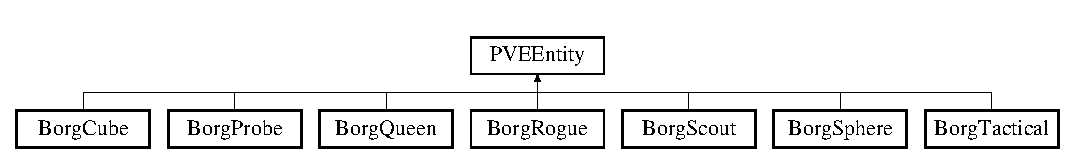
\includegraphics[height=1.75824cm]{df/dde/classPVEEntity}
\end{center}
\end{figure}
\subsection*{Public Member Functions}
\begin{DoxyCompactItemize}
\item 
\hyperlink{classPVEEntity_ab00e5efa6fb12a9661df9a1c74c72168}{PVEEntity} ()
\item 
virtual \hyperlink{classPVEEntity_aac5b1b2d4ecf705c32734907741d56d2}{$\sim$PVEEntity} ()
\item 
\hypertarget{classPVEEntity_abd5e859d332c2920f005ef8c97734dff}{
virtual string {\bfseries getName} ()=0}
\label{df/dde/classPVEEntity_abd5e859d332c2920f005ef8c97734dff}

\item 
\hypertarget{classPVEEntity_a352a032772da3a69481f382c85db0cf6}{
virtual int {\bfseries getShieldStrenght} ()=0}
\label{df/dde/classPVEEntity_a352a032772da3a69481f382c85db0cf6}

\item 
\hypertarget{classPVEEntity_a4652096367bb38b3635c39015b6be341}{
virtual int {\bfseries getShieldRegenerativeRate} ()=0}
\label{df/dde/classPVEEntity_a4652096367bb38b3635c39015b6be341}

\item 
\hypertarget{classPVEEntity_aa36eeaf1c2e0eabadd6d64e2a7ef4886}{
virtual int {\bfseries getRegenerativeAdaptivePlating} ()=0}
\label{df/dde/classPVEEntity_aa36eeaf1c2e0eabadd6d64e2a7ef4886}

\item 
\hypertarget{classPVEEntity_a411d1158d184f4912420fc49b6d03209}{
virtual bool {\bfseries getHasRegenerativeAdaptivePlating} ()=0}
\label{df/dde/classPVEEntity_a411d1158d184f4912420fc49b6d03209}

\item 
\hypertarget{classPVEEntity_a865254bdecac68ca01cb010c7ac22a03}{
virtual int {\bfseries getTransPhasicTorpedos} ()=0}
\label{df/dde/classPVEEntity_a865254bdecac68ca01cb010c7ac22a03}

\item 
\hypertarget{classPVEEntity_a95362dd29a50832c268f0a465fb0c3b7}{
virtual bool {\bfseries getHasTransphasicTorpedos} ()=0}
\label{df/dde/classPVEEntity_a95362dd29a50832c268f0a465fb0c3b7}

\item 
\hypertarget{classPVEEntity_a2231dfd422613018b41903197abe4098}{
virtual int {\bfseries getChronitonTorpedos} ()=0}
\label{df/dde/classPVEEntity_a2231dfd422613018b41903197abe4098}

\item 
\hypertarget{classPVEEntity_a34f008af67cfe98cf4db0f7e4e56aa8a}{
virtual bool {\bfseries getHasChronitonTorpedos} ()=0}
\label{df/dde/classPVEEntity_a34f008af67cfe98cf4db0f7e4e56aa8a}

\item 
\hypertarget{classPVEEntity_a699bdbd6f4f04f722cf463322924c3d7}{
virtual int {\bfseries getGravimetricTorpedos} ()=0}
\label{df/dde/classPVEEntity_a699bdbd6f4f04f722cf463322924c3d7}

\item 
\hypertarget{classPVEEntity_ac4ccef560d2f3116d25a991adcf29160}{
virtual bool {\bfseries getHasGravimetricTorpedos} ()=0}
\label{df/dde/classPVEEntity_ac4ccef560d2f3116d25a991adcf29160}

\item 
\hypertarget{classPVEEntity_a954f89529da48c1219d356003ea7bf9e}{
virtual int {\bfseries getSpatialTorpedos} ()=0}
\label{df/dde/classPVEEntity_a954f89529da48c1219d356003ea7bf9e}

\item 
\hypertarget{classPVEEntity_a0e6303e47a9989533246050d485a3269}{
virtual bool {\bfseries getHasSpatialTorpedos} ()=0}
\label{df/dde/classPVEEntity_a0e6303e47a9989533246050d485a3269}

\item 
\hypertarget{classPVEEntity_a70d57d0a3a2bf457b4773f15a32e3611}{
virtual bool {\bfseries getHasLasers} ()=0}
\label{df/dde/classPVEEntity_a70d57d0a3a2bf457b4773f15a32e3611}

\item 
\hypertarget{classPVEEntity_a3860cee61b565228e2ae06f46dc91ae0}{
virtual bool {\bfseries getHasPhasedIonCannon} ()=0}
\label{df/dde/classPVEEntity_a3860cee61b565228e2ae06f46dc91ae0}

\item 
\hypertarget{classPVEEntity_a84ba088b68a8405d7e77230b17133210}{
virtual bool {\bfseries getHasPulseWeapon} ()=0}
\label{df/dde/classPVEEntity_a84ba088b68a8405d7e77230b17133210}

\item 
\hypertarget{classPVEEntity_ae5222ad066788fccef43d5d18fd144ea}{
virtual int {\bfseries getBorgComplement} ()=0}
\label{df/dde/classPVEEntity_ae5222ad066788fccef43d5d18fd144ea}

\item 
\hypertarget{classPVEEntity_af2b571ab647e6442e8b1d51748ac8ac4}{
virtual bool {\bfseries getHasTractorLock} ()=0}
\label{df/dde/classPVEEntity_af2b571ab647e6442e8b1d51748ac8ac4}

\item 
\hypertarget{classPVEEntity_a8e8c12e80b764f737e26045ab55ba62f}{
virtual bool {\bfseries getIsWreckPVE} ()=0}
\label{df/dde/classPVEEntity_a8e8c12e80b764f737e26045ab55ba62f}

\item 
\hypertarget{classPVEEntity_a9ff78957a31e68087dda157baefaebdc}{
virtual void {\bfseries setShieldStrenghtPVE} (int strenght)=0}
\label{df/dde/classPVEEntity_a9ff78957a31e68087dda157baefaebdc}

\item 
\hypertarget{classPVEEntity_a6a17717e26c57959e66a628ecd9bcabf}{
virtual void {\bfseries setShieldRegenerativeRatePVE} (int rate)=0}
\label{df/dde/classPVEEntity_a6a17717e26c57959e66a628ecd9bcabf}

\item 
\hypertarget{classPVEEntity_af16d2b1fc5173c5f7d1e4756bc37d775}{
virtual void {\bfseries setArmourPVE} (int armour)=0}
\label{df/dde/classPVEEntity_af16d2b1fc5173c5f7d1e4756bc37d775}

\item 
\hypertarget{classPVEEntity_a4458ff9d27d95be5e4d8e7d237bc74b9}{
virtual void {\bfseries setTransPhasicTorpedosPVE} (int num)=0}
\label{df/dde/classPVEEntity_a4458ff9d27d95be5e4d8e7d237bc74b9}

\item 
\hypertarget{classPVEEntity_acc7496844abcbb993e84ca115f910fc1}{
virtual void {\bfseries setChronitonTorpedosPVE} (int num)=0}
\label{df/dde/classPVEEntity_acc7496844abcbb993e84ca115f910fc1}

\item 
\hypertarget{classPVEEntity_aa1163c04929940d1127fc01d1933710a}{
virtual void {\bfseries setGravimetricTorpedosPVE} (int num)=0}
\label{df/dde/classPVEEntity_aa1163c04929940d1127fc01d1933710a}

\item 
\hypertarget{classPVEEntity_aa9dfb8aec3a3ebc3c7a9c7ff3935ef1b}{
virtual void {\bfseries setSpatialTorpedosPVE} (int num)=0}
\label{df/dde/classPVEEntity_aa9dfb8aec3a3ebc3c7a9c7ff3935ef1b}

\item 
\hypertarget{classPVEEntity_a9d84e2dfe23bfa674d729566a4dc8033}{
virtual void {\bfseries setHasTractorLockPVE} (bool has)=0}
\label{df/dde/classPVEEntity_a9d84e2dfe23bfa674d729566a4dc8033}

\item 
\hypertarget{classPVEEntity_a072bbcc0e8db91cc27a63d22aafd8904}{
virtual void {\bfseries setWreckPVE} ()=0}
\label{df/dde/classPVEEntity_a072bbcc0e8db91cc27a63d22aafd8904}

\end{DoxyCompactItemize}
\subsection*{Protected Attributes}
\begin{DoxyCompactItemize}
\item 
\hypertarget{classPVEEntity_a9350ded0194abfcd72d85abbfbecbd32}{
string {\bfseries type}}
\label{df/dde/classPVEEntity_a9350ded0194abfcd72d85abbfbecbd32}

\item 
\hypertarget{classPVEEntity_addcf75561353a6ef431d43885a151e1d}{
int {\bfseries regenerativeAdaptivePlating}}
\label{df/dde/classPVEEntity_addcf75561353a6ef431d43885a151e1d}

\item 
\hypertarget{classPVEEntity_ae3d2015f8baac0f8fc212161c1517446}{
bool {\bfseries hasRegenerativeAdaptivePlating}}
\label{df/dde/classPVEEntity_ae3d2015f8baac0f8fc212161c1517446}

\item 
\hypertarget{classPVEEntity_a396fed8d6238852b66352d695ed11883}{
int {\bfseries shieldStrenght}}
\label{df/dde/classPVEEntity_a396fed8d6238852b66352d695ed11883}

\item 
\hypertarget{classPVEEntity_a94f93d1a9277d988065f82343e93ba8e}{
int {\bfseries shieldRegenerativeRate}}
\label{df/dde/classPVEEntity_a94f93d1a9277d988065f82343e93ba8e}

\item 
\hypertarget{classPVEEntity_a973f8c6a700bf7cb6fb79c0a56605b07}{
int {\bfseries transPhasicTorpedos}}
\label{df/dde/classPVEEntity_a973f8c6a700bf7cb6fb79c0a56605b07}

\item 
\hypertarget{classPVEEntity_ae4a171aac4f61a935851caaf34b95a47}{
bool {\bfseries hasTransPhasicTorpedos}}
\label{df/dde/classPVEEntity_ae4a171aac4f61a935851caaf34b95a47}

\item 
\hypertarget{classPVEEntity_a2e5c5228cc55b72ab8b040f09633efd0}{
int {\bfseries chronitonTorpedos}}
\label{df/dde/classPVEEntity_a2e5c5228cc55b72ab8b040f09633efd0}

\item 
\hypertarget{classPVEEntity_a38f6e378fee4c59841aaeddab9aed149}{
bool {\bfseries hasChronitonTorpedos}}
\label{df/dde/classPVEEntity_a38f6e378fee4c59841aaeddab9aed149}

\item 
\hypertarget{classPVEEntity_a9b7aba9f178363860fa037a8b763360f}{
int {\bfseries gravimetricTorpedos}}
\label{df/dde/classPVEEntity_a9b7aba9f178363860fa037a8b763360f}

\item 
\hypertarget{classPVEEntity_a30c90638b1e57ef820bc49d399898e62}{
bool {\bfseries hasGravimetricTorpedos}}
\label{df/dde/classPVEEntity_a30c90638b1e57ef820bc49d399898e62}

\item 
\hypertarget{classPVEEntity_ab3a93dc87abe710c0454dab72e797501}{
int {\bfseries spatialTorpedos}}
\label{df/dde/classPVEEntity_ab3a93dc87abe710c0454dab72e797501}

\item 
\hypertarget{classPVEEntity_ad41be3eb468b1e319939725cef5150ad}{
bool {\bfseries hasSpatialTorpedos}}
\label{df/dde/classPVEEntity_ad41be3eb468b1e319939725cef5150ad}

\item 
\hypertarget{classPVEEntity_aee171ddedafdfb62b223fecccfedc2e4}{
bool {\bfseries hasLasers}}
\label{df/dde/classPVEEntity_aee171ddedafdfb62b223fecccfedc2e4}

\item 
\hypertarget{classPVEEntity_a25b855c72a189accf086eb49525b2a5f}{
bool {\bfseries hasPhasedIonCannon}}
\label{df/dde/classPVEEntity_a25b855c72a189accf086eb49525b2a5f}

\item 
\hypertarget{classPVEEntity_a8eadbf974fc1aa6618b39cf20d133198}{
bool {\bfseries hasPulseWeapon}}
\label{df/dde/classPVEEntity_a8eadbf974fc1aa6618b39cf20d133198}

\item 
\hypertarget{classPVEEntity_aa94b966b7af3165fd5e3282097702806}{
int {\bfseries borgDrones}}
\label{df/dde/classPVEEntity_aa94b966b7af3165fd5e3282097702806}

\item 
\hypertarget{classPVEEntity_a15fdb119f59dfd1cdc72692815f90e5b}{
bool {\bfseries hasTractorLock}}
\label{df/dde/classPVEEntity_a15fdb119f59dfd1cdc72692815f90e5b}

\item 
\hypertarget{classPVEEntity_a566abd3a5281d4924ed23979ae1b1af4}{
bool {\bfseries isWreck}}
\label{df/dde/classPVEEntity_a566abd3a5281d4924ed23979ae1b1af4}

\end{DoxyCompactItemize}


\subsection{Constructor \& Destructor Documentation}
\hypertarget{classPVEEntity_ab00e5efa6fb12a9661df9a1c74c72168}{
\index{PVEEntity@{PVEEntity}!PVEEntity@{PVEEntity}}
\index{PVEEntity@{PVEEntity}!PVEEntity@{PVEEntity}}
\subsubsection[{PVEEntity}]{\setlength{\rightskip}{0pt plus 5cm}PVEEntity::PVEEntity ()}}
\label{df/dde/classPVEEntity_ab00e5efa6fb12a9661df9a1c74c72168}
Constructor for pve entity sets up data embers based on preloaded variables arrays usning random index adds itself to the all game enemies vector \hypertarget{classPVEEntity_aac5b1b2d4ecf705c32734907741d56d2}{
\index{PVEEntity@{PVEEntity}!$\sim$PVEEntity@{$\sim$PVEEntity}}
\index{$\sim$PVEEntity@{$\sim$PVEEntity}!PVEEntity@{PVEEntity}}
\subsubsection[{$\sim$PVEEntity}]{\setlength{\rightskip}{0pt plus 5cm}PVEEntity::$\sim$PVEEntity ()\hspace{0.3cm}{\ttfamily  \mbox{[}virtual\mbox{]}}}}
\label{df/dde/classPVEEntity_aac5b1b2d4ecf705c32734907741d56d2}
Destructor for the enemy 

The documentation for this class was generated from the following files:\begin{DoxyCompactItemize}
\item 
source/header/PVEEntity.h\item 
source/source/PVEEntity.cpp\end{DoxyCompactItemize}

\hypertarget{classSdlGLMap}{
\section{SdlGLMap Class Reference}
\label{d9/d4a/classSdlGLMap}\index{SdlGLMap@{SdlGLMap}}
}
\subsection*{Public Member Functions}
\begin{DoxyCompactItemize}
\item 
\hyperlink{classSdlGLMap_a8f8c64f935f9604c1d4874bcc0c7ca0d}{SdlGLMap} ()
\item 
\hyperlink{classSdlGLMap_a772938300f573106c2a124487250b273}{$\sim$SdlGLMap} ()
\end{DoxyCompactItemize}


\subsection{Constructor \& Destructor Documentation}
\hypertarget{classSdlGLMap_a8f8c64f935f9604c1d4874bcc0c7ca0d}{
\index{SdlGLMap@{SdlGLMap}!SdlGLMap@{SdlGLMap}}
\index{SdlGLMap@{SdlGLMap}!SdlGLMap@{SdlGLMap}}
\subsubsection[{SdlGLMap}]{\setlength{\rightskip}{0pt plus 5cm}SdlGLMap::SdlGLMap ()}}
\label{d9/d4a/classSdlGLMap_a8f8c64f935f9604c1d4874bcc0c7ca0d}
Constructor

Loads Surface Bitmaps, Mix\_\-chunk Sounds \hypertarget{classSdlGLMap_a772938300f573106c2a124487250b273}{
\index{SdlGLMap@{SdlGLMap}!$\sim$SdlGLMap@{$\sim$SdlGLMap}}
\index{$\sim$SdlGLMap@{$\sim$SdlGLMap}!SdlGLMap@{SdlGLMap}}
\subsubsection[{$\sim$SdlGLMap}]{\setlength{\rightskip}{0pt plus 5cm}SdlGLMap::$\sim$SdlGLMap ()}}
\label{d9/d4a/classSdlGLMap_a772938300f573106c2a124487250b273}
Destructor

Releases Surfaces, Mix\_\-Chunks Releases Audio \& Video subsystem 

The documentation for this class was generated from the following files:\begin{DoxyCompactItemize}
\item 
source/header/SdlGLMap.h\item 
source/source/SdlGLMap.cpp\end{DoxyCompactItemize}

\hypertarget{classSolarSystem}{
\section{SolarSystem Class Reference}
\label{df/d5e/classSolarSystem}\index{SolarSystem@{SolarSystem}}
}
\subsection*{Public Member Functions}
\begin{DoxyCompactItemize}
\item 
\hyperlink{classSolarSystem_a459f5b68b920b9816788e76b6a821488}{SolarSystem} (string name, \hyperlink{classStarTrekEntities}{StarTrekEntities} $\ast$stePointer, unsigned int gameDifficulty)
\item 
\hyperlink{classSolarSystem_ac520dce0faa7df3755326fb2b6f7b51a}{$\sim$SolarSystem} ()
\item 
void \hyperlink{classSolarSystem_a1d7fdbf5b11c2f4cd9b8151390e268a7}{setExits} (\hyperlink{classSolarSystem}{SolarSystem} $\ast$ahead, \hyperlink{classSolarSystem}{SolarSystem} $\ast$port, \hyperlink{classSolarSystem}{SolarSystem} $\ast$back, \hyperlink{classSolarSystem}{SolarSystem} $\ast$starboard)
\item 
string \hyperlink{classSolarSystem_a8493fd255139bae07453818facfe52ce}{getName} ()
\item 
\hyperlink{classSolarSystem}{SolarSystem} $\ast$ \hyperlink{classSolarSystem_a65d3cebc039c25bc4427f72fb20c890c}{nextSolarSystem} (string direction)
\item 
\hyperlink{classCelestialBody}{CelestialBody} $\ast$ \hyperlink{classSolarSystem_a149b4356b3dd7da090b33dc699cc9b7c}{targetPlanet} (unsigned int i)
\item 
\hyperlink{classPVEEntity}{PVEEntity} $\ast$ \hyperlink{classSolarSystem_a92a2a0ae9e987e32e65c46d207a868d7}{targetPVEEntity} (unsigned int pve\_\-i)
\item 
\hyperlink{classCelestialBody}{CelestialBody} $\ast$ \hyperlink{classSolarSystem_af1511d3f14b0be819941f585fef039a0}{targetPlanetMoon} (unsigned int planet\_\-i, unsigned int moon\_\-i)
\item 
void \hyperlink{classSolarSystem_a7be656472d3867ed7eb416da51982463}{scanPlanet} (unsigned int i)
\item 
void \hyperlink{classSolarSystem_a7d9d47e7b7a987f4d2bad4ebe40ac911}{scanPlanetMoon} (unsigned int planet\_\-i, unsigned int moon\_\-i)
\item 
void \hyperlink{classSolarSystem_a92596df0b4af0f979c06f3de7685a74c}{scanPVEEntity} (unsigned int pve\_\-i)
\item 
vector$<$ \hyperlink{classPVEEntity}{PVEEntity} $\ast$ $>$ \hyperlink{classSolarSystem_a4743c88ee83ef7ae0ed3a308004179bb}{getPVEEntity} ()
\item 
vector$<$ \hyperlink{classCelestialBody}{CelestialBody} $\ast$ $>$ \hyperlink{classSolarSystem_a334394234a898ccb7b35ee0f2ab8e648}{getSystemPlanets} ()
\item 
\hyperlink{classPVEEntity}{PVEEntity} $\ast$ \hyperlink{classSolarSystem_a6f30ebe96f6ef56d967f3e6c368057d2}{randomAttack} (unsigned int difficulty)
\item 
void \hyperlink{classSolarSystem_a891417265b57aa785bd808fc7a2485c4}{scanSystem} ()
\item 
void \hyperlink{classSolarSystem_a1efb6ebd3741f3fce2f5cb7d1eeffc19}{moveEnemies} ()
\item 
void \hyperlink{classSolarSystem_a95839db98d8dbf297536fba1aae7f2a6}{addEnemy} (\hyperlink{classPVEEntity}{PVEEntity} $\ast$visitor)
\item 
void \hyperlink{classSolarSystem_a41f1cdf83a580bd2258d9233ef0cdb4f}{operator-\/-\/} ()
\end{DoxyCompactItemize}


\subsection{Constructor \& Destructor Documentation}
\hypertarget{classSolarSystem_a459f5b68b920b9816788e76b6a821488}{
\index{SolarSystem@{SolarSystem}!SolarSystem@{SolarSystem}}
\index{SolarSystem@{SolarSystem}!SolarSystem@{SolarSystem}}
\subsubsection[{SolarSystem}]{\setlength{\rightskip}{0pt plus 5cm}SolarSystem::SolarSystem (string {\em name}, \/  {\bf StarTrekEntities} $\ast$ {\em stePointer}, \/  unsigned int {\em gameDifficulty})}}
\label{df/d5e/classSolarSystem_a459f5b68b920b9816788e76b6a821488}
Constructor for Solarsystem


\begin{DoxyParams}{Parameters}
\item[{\em name}]the name of the solar system \item[{\em stePointer}]pointer to the \hyperlink{classStarTrekEntities}{StarTrekEntities} object names from file) \item[{\em gameDifficulty}]the game difficulty of the game \end{DoxyParams}
\hypertarget{classSolarSystem_ac520dce0faa7df3755326fb2b6f7b51a}{
\index{SolarSystem@{SolarSystem}!$\sim$SolarSystem@{$\sim$SolarSystem}}
\index{$\sim$SolarSystem@{$\sim$SolarSystem}!SolarSystem@{SolarSystem}}
\subsubsection[{$\sim$SolarSystem}]{\setlength{\rightskip}{0pt plus 5cm}SolarSystem::$\sim$SolarSystem ()}}
\label{df/d5e/classSolarSystem_ac520dce0faa7df3755326fb2b6f7b51a}
destructor for the solar system deletes the pointers to the planets and PVEentities 

\subsection{Member Function Documentation}
\hypertarget{classSolarSystem_a95839db98d8dbf297536fba1aae7f2a6}{
\index{SolarSystem@{SolarSystem}!addEnemy@{addEnemy}}
\index{addEnemy@{addEnemy}!SolarSystem@{SolarSystem}}
\subsubsection[{addEnemy}]{\setlength{\rightskip}{0pt plus 5cm}void SolarSystem::addEnemy ({\bf PVEEntity} $\ast$ {\em visitor})}}
\label{df/d5e/classSolarSystem_a95839db98d8dbf297536fba1aae7f2a6}
Takes an enemy pointer and adds it to this system Used in conjunction with enemy movement


\begin{DoxyParams}{Parameters}
\item[{\em visitor}]the enemy pointer \end{DoxyParams}
\hypertarget{classSolarSystem_a8493fd255139bae07453818facfe52ce}{
\index{SolarSystem@{SolarSystem}!getName@{getName}}
\index{getName@{getName}!SolarSystem@{SolarSystem}}
\subsubsection[{getName}]{\setlength{\rightskip}{0pt plus 5cm}string SolarSystem::getName ()}}
\label{df/d5e/classSolarSystem_a8493fd255139bae07453818facfe52ce}
gets the name of this solar system

\begin{DoxyReturn}{Returns}
string the name of the solarsystem 
\end{DoxyReturn}
\hypertarget{classSolarSystem_a4743c88ee83ef7ae0ed3a308004179bb}{
\index{SolarSystem@{SolarSystem}!getPVEEntity@{getPVEEntity}}
\index{getPVEEntity@{getPVEEntity}!SolarSystem@{SolarSystem}}
\subsubsection[{getPVEEntity}]{\setlength{\rightskip}{0pt plus 5cm}vector$<$ {\bf PVEEntity} $\ast$ $>$ SolarSystem::getPVEEntity ()}}
\label{df/d5e/classSolarSystem_a4743c88ee83ef7ae0ed3a308004179bb}
returns a copy of the PVE vector

\begin{DoxyReturn}{Returns}
vector$<$PVEEntity$\ast$$>$ 
\end{DoxyReturn}
\hypertarget{classSolarSystem_a334394234a898ccb7b35ee0f2ab8e648}{
\index{SolarSystem@{SolarSystem}!getSystemPlanets@{getSystemPlanets}}
\index{getSystemPlanets@{getSystemPlanets}!SolarSystem@{SolarSystem}}
\subsubsection[{getSystemPlanets}]{\setlength{\rightskip}{0pt plus 5cm}vector$<$ {\bf CelestialBody} $\ast$ $>$ SolarSystem::getSystemPlanets ()}}
\label{df/d5e/classSolarSystem_a334394234a898ccb7b35ee0f2ab8e648}
returns a copy of the planets vector

\begin{DoxyReturn}{Returns}
vector$<$CelestialBody$\ast$$>$ 
\end{DoxyReturn}
\hypertarget{classSolarSystem_a1efb6ebd3741f3fce2f5cb7d1eeffc19}{
\index{SolarSystem@{SolarSystem}!moveEnemies@{moveEnemies}}
\index{moveEnemies@{moveEnemies}!SolarSystem@{SolarSystem}}
\subsubsection[{moveEnemies}]{\setlength{\rightskip}{0pt plus 5cm}void SolarSystem::moveEnemies ()}}
\label{df/d5e/classSolarSystem_a1efb6ebd3741f3fce2f5cb7d1eeffc19}
Moves enemies form this solar system to another

\begin{DoxyReturn}{Returns}
void 
\end{DoxyReturn}
\hypertarget{classSolarSystem_a65d3cebc039c25bc4427f72fb20c890c}{
\index{SolarSystem@{SolarSystem}!nextSolarSystem@{nextSolarSystem}}
\index{nextSolarSystem@{nextSolarSystem}!SolarSystem@{SolarSystem}}
\subsubsection[{nextSolarSystem}]{\setlength{\rightskip}{0pt plus 5cm}{\bf SolarSystem} $\ast$ SolarSystem::nextSolarSystem (string {\em direction})}}
\label{df/d5e/classSolarSystem_a65d3cebc039c25bc4427f72fb20c890c}
returns the exit to the requested solar system or null if it does not have an exit in that direction


\begin{DoxyParams}{Parameters}
\item[{\em direction}]to travel\end{DoxyParams}
\begin{DoxyReturn}{Returns}
the pointer to the directed solarsystem or null 
\end{DoxyReturn}
\hypertarget{classSolarSystem_a41f1cdf83a580bd2258d9233ef0cdb4f}{
\index{SolarSystem@{SolarSystem}!operator-\/-\/@{operator-\/-\/}}
\index{operator-\/-\/@{operator-\/-\/}!SolarSystem@{SolarSystem}}
\subsubsection[{operator-\/-\/}]{\setlength{\rightskip}{0pt plus 5cm}void SolarSystem::operator-\/-\/ ()}}
\label{df/d5e/classSolarSystem_a41f1cdf83a580bd2258d9233ef0cdb4f}
Seriously bad example of operator overloading

\begin{DoxyReturn}{Returns}
void 
\end{DoxyReturn}
\hypertarget{classSolarSystem_a6f30ebe96f6ef56d967f3e6c368057d2}{
\index{SolarSystem@{SolarSystem}!randomAttack@{randomAttack}}
\index{randomAttack@{randomAttack}!SolarSystem@{SolarSystem}}
\subsubsection[{randomAttack}]{\setlength{\rightskip}{0pt plus 5cm}{\bf PVEEntity} $\ast$ SolarSystem::randomAttack (unsigned int {\em difficulty})}}
\label{df/d5e/classSolarSystem_a6f30ebe96f6ef56d967f3e6c368057d2}
once you enter into this solar system enemies will attack based upon the game difficulty


\begin{DoxyParams}{Parameters}
\item[{\em difficulty}]the game difficulty\end{DoxyParams}
\begin{DoxyReturn}{Returns}
a pointer to a \hyperlink{classPVEEntity}{PVEEntity} or null 
\end{DoxyReturn}
\hypertarget{classSolarSystem_a7be656472d3867ed7eb416da51982463}{
\index{SolarSystem@{SolarSystem}!scanPlanet@{scanPlanet}}
\index{scanPlanet@{scanPlanet}!SolarSystem@{SolarSystem}}
\subsubsection[{scanPlanet}]{\setlength{\rightskip}{0pt plus 5cm}void SolarSystem::scanPlanet (unsigned int {\em i})}}
\label{df/d5e/classSolarSystem_a7be656472d3867ed7eb416da51982463}
prints out information about a planet in this solar system


\begin{DoxyParams}{Parameters}
\item[{\em i}]the planet to scan\end{DoxyParams}
\begin{DoxyReturn}{Returns}
void 
\end{DoxyReturn}
\hypertarget{classSolarSystem_a7d9d47e7b7a987f4d2bad4ebe40ac911}{
\index{SolarSystem@{SolarSystem}!scanPlanetMoon@{scanPlanetMoon}}
\index{scanPlanetMoon@{scanPlanetMoon}!SolarSystem@{SolarSystem}}
\subsubsection[{scanPlanetMoon}]{\setlength{\rightskip}{0pt plus 5cm}void SolarSystem::scanPlanetMoon (unsigned int {\em planet\_\-i}, \/  unsigned int {\em moon\_\-i})}}
\label{df/d5e/classSolarSystem_a7d9d47e7b7a987f4d2bad4ebe40ac911}
calls a planets moon and pointer out information about it in the function called


\begin{DoxyParams}{Parameters}
\item[{\em planet\_\-i}]the planet that the moon belongs too \item[{\em moon\_\-i}]the moon belong to the planet\end{DoxyParams}
\begin{DoxyReturn}{Returns}
void 
\end{DoxyReturn}
\hypertarget{classSolarSystem_a92596df0b4af0f979c06f3de7685a74c}{
\index{SolarSystem@{SolarSystem}!scanPVEEntity@{scanPVEEntity}}
\index{scanPVEEntity@{scanPVEEntity}!SolarSystem@{SolarSystem}}
\subsubsection[{scanPVEEntity}]{\setlength{\rightskip}{0pt plus 5cm}void SolarSystem::scanPVEEntity (unsigned int {\em pve\_\-i})}}
\label{df/d5e/classSolarSystem_a92596df0b4af0f979c06f3de7685a74c}
prints out information about the selected pve in this solarsystem


\begin{DoxyParams}{Parameters}
\item[{\em pve\_\-i}]the pve in the vector to scan\end{DoxyParams}
\begin{DoxyReturn}{Returns}
void 
\end{DoxyReturn}
\hypertarget{classSolarSystem_a891417265b57aa785bd808fc7a2485c4}{
\index{SolarSystem@{SolarSystem}!scanSystem@{scanSystem}}
\index{scanSystem@{scanSystem}!SolarSystem@{SolarSystem}}
\subsubsection[{scanSystem}]{\setlength{\rightskip}{0pt plus 5cm}void SolarSystem::scanSystem ()}}
\label{df/d5e/classSolarSystem_a891417265b57aa785bd808fc7a2485c4}
prints out information about this solar system including enemies, planets \& their moons

\begin{DoxyReturn}{Returns}
void 
\end{DoxyReturn}
\hypertarget{classSolarSystem_a1d7fdbf5b11c2f4cd9b8151390e268a7}{
\index{SolarSystem@{SolarSystem}!setExits@{setExits}}
\index{setExits@{setExits}!SolarSystem@{SolarSystem}}
\subsubsection[{setExits}]{\setlength{\rightskip}{0pt plus 5cm}void SolarSystem::setExits ({\bf SolarSystem} $\ast$ {\em ahead}, \/  {\bf SolarSystem} $\ast$ {\em port}, \/  {\bf SolarSystem} $\ast$ {\em back}, \/  {\bf SolarSystem} $\ast$ {\em starboard})}}
\label{df/d5e/classSolarSystem_a1d7fdbf5b11c2f4cd9b8151390e268a7}
sets the exits for the solar system


\begin{DoxyParams}{Parameters}
\item[{\em ahead}]pointer to a solarsystem \item[{\em port}]pointer to a solarsystem \item[{\em back}]pointer to a solarsystem \item[{\em starboard}]pointer to a solarsystem\end{DoxyParams}
\begin{DoxyReturn}{Returns}
void 
\end{DoxyReturn}
\hypertarget{classSolarSystem_a149b4356b3dd7da090b33dc699cc9b7c}{
\index{SolarSystem@{SolarSystem}!targetPlanet@{targetPlanet}}
\index{targetPlanet@{targetPlanet}!SolarSystem@{SolarSystem}}
\subsubsection[{targetPlanet}]{\setlength{\rightskip}{0pt plus 5cm}{\bf CelestialBody} $\ast$ SolarSystem::targetPlanet (unsigned int {\em i})}}
\label{df/d5e/classSolarSystem_a149b4356b3dd7da090b33dc699cc9b7c}
if a target is request for this solar system planet, check to see if it exists first and return a pointer to the object


\begin{DoxyParams}{Parameters}
\item[{\em i}]the planet to target in the vector\end{DoxyParams}
\begin{DoxyReturn}{Returns}
pointer to CelestialBody(planet) or null 
\end{DoxyReturn}
\hypertarget{classSolarSystem_af1511d3f14b0be819941f585fef039a0}{
\index{SolarSystem@{SolarSystem}!targetPlanetMoon@{targetPlanetMoon}}
\index{targetPlanetMoon@{targetPlanetMoon}!SolarSystem@{SolarSystem}}
\subsubsection[{targetPlanetMoon}]{\setlength{\rightskip}{0pt plus 5cm}{\bf CelestialBody} $\ast$ SolarSystem::targetPlanetMoon (unsigned int {\em planet\_\-i}, \/  unsigned int {\em moon\_\-i})}}
\label{df/d5e/classSolarSystem_af1511d3f14b0be819941f585fef039a0}
if a target is request for this solar system moon, check to see if it exists first and return a pointer to the object


\begin{DoxyParams}{Parameters}
\item[{\em planet\_\-i}]the planet that the moon belongs too \item[{\em moon\_\-i}]the moon belong to the planet\end{DoxyParams}
\begin{DoxyReturn}{Returns}
a pointer to the \hyperlink{classCelestialBody}{CelestialBody} (moon) 
\end{DoxyReturn}
\hypertarget{classSolarSystem_a92a2a0ae9e987e32e65c46d207a868d7}{
\index{SolarSystem@{SolarSystem}!targetPVEEntity@{targetPVEEntity}}
\index{targetPVEEntity@{targetPVEEntity}!SolarSystem@{SolarSystem}}
\subsubsection[{targetPVEEntity}]{\setlength{\rightskip}{0pt plus 5cm}{\bf PVEEntity} $\ast$ SolarSystem::targetPVEEntity (unsigned int {\em pve\_\-i})}}
\label{df/d5e/classSolarSystem_a92a2a0ae9e987e32e65c46d207a868d7}
if a target is request for this solar system pve entity, check to see if it exists first and return a pointer to the object


\begin{DoxyParams}{Parameters}
\item[{\em pve\_\-i}]the pve entiry to target\end{DoxyParams}
\begin{DoxyReturn}{Returns}
a pointer to a \hyperlink{classPVEEntity}{PVEEntity} or null 
\end{DoxyReturn}


The documentation for this class was generated from the following files:\begin{DoxyCompactItemize}
\item 
source/header/SolarSystem.h\item 
source/source/SolarSystem.cpp\end{DoxyCompactItemize}

\hypertarget{classStarShip}{
\section{StarShip Class Reference}
\label{da/d97/classStarShip}\index{StarShip@{StarShip}}
}
\subsection*{Public Member Functions}
\begin{DoxyCompactItemize}
\item 
\hyperlink{classStarShip_a616271a6df7759753f1919e1e244744e}{StarShip} (string name, int gameDifficulty)
\item 
\hyperlink{classStarShip_a334de38a2a083eeaf2e509f403db3124}{$\sim$StarShip} ()
\item 
string \hyperlink{classStarShip_a822cba8f4276378a9c4cec72213e1e80}{getName} ()
\item 
int \hyperlink{classStarShip_a34a3514784bb0bdb7a7688c5ff6ad033}{getShieldStrenght} ()
\item 
int \hyperlink{classStarShip_a6c5cf11fb023e98a6e23d7be9d41a984}{getShieldRegenerativeRate} ()
\item 
int \hyperlink{classStarShip_aaa27c8e41243ff314a53aa7d1c625456}{getArmour} ()
\item 
int \hyperlink{classStarShip_a48df1266b1b5d8ed36ad91bc0ac8e53b}{getPhotons} ()
\item 
int \hyperlink{classStarShip_a5859482046dae7a0ac2ad18c5714f6eb}{getQuantums} ()
\item 
int \hyperlink{classStarShip_a3bdba9448b3c6096f6973abccf2eca0c}{getPower} ()
\item 
int \hyperlink{classStarShip_af770b4878c7b724d96c0ed4e7d13c0fa}{getFood} ()
\item 
int \hyperlink{classStarShip_a83cb2a208ff3e0925671ab853679c400}{getWater} ()
\item 
int \hyperlink{classStarShip_a9da23f7827b3f10fb22b3b0e4cea8e52}{getPlasma} ()
\item 
int \hyperlink{classStarShip_a2cc968a0cf44328b29d79e7d4c30c013}{getTrianium} ()
\item 
int \hyperlink{classStarShip_a3c371aaeccfab3f6e406a14d25daca18}{getDilithium} ()
\item 
int \hyperlink{classStarShip_ac166ff73eb10a460810bfe3c190a24e3}{getCargoWeight} ()
\item 
bool \hyperlink{classStarShip_af072da551eff3b24cce85dd5f33efba3}{getHasTractorLock} ()
\item 
bool \hyperlink{classStarShip_ac0a6b7de51c9b461ca186d1412f4208f}{getIsWreck} ()
\item 
void \hyperlink{classStarShip_abe926e5606f91d6ec80b6779fee16e39}{setShieldStrenght} (int strenght)
\item 
void \hyperlink{classStarShip_a9b41a780259b41ebec4b69de12ecc276}{setShieldRegenerativeRate} (int rate)
\item 
void \hyperlink{classStarShip_a599c3c86e50738951fc468544fa916e4}{setArmour} (int armour)
\item 
void \hyperlink{classStarShip_a207cd846544ef333a25b14d737fa934a}{setPhotons} (int num)
\item 
void \hyperlink{classStarShip_a54668a25efe99edc19892e3433008843}{setQuantums} (int num)
\item 
void \hyperlink{classStarShip_a3e690a6c422f5d863086536313d68bb9}{setPower} (int num)
\item 
void \hyperlink{classStarShip_a5c1681ff3b6d20aa7cbb6bce36ab74fe}{setFood} (int val)
\item 
void \hyperlink{classStarShip_a61a1341a3e3640eea186cedae52fbd0e}{setWater} (int val)
\item 
void \hyperlink{classStarShip_afb3ed2798519853ab293432604e4fb0c}{setPlasma} (int val, bool transporter)
\item 
void \hyperlink{classStarShip_a77b32c7f2290cafd2827b868c962d6e9}{setTrianium} (int val)
\item 
void \hyperlink{classStarShip_a99530aa5ae4093bc75d5df1efa5dbdde}{setDilithium} (int val)
\item 
void \hyperlink{classStarShip_ad1a29b9f7ee09f56a78b9994830241b6}{updateCargoWeight} ()
\item 
void \hyperlink{classStarShip_a44bc85e4cbd29a883d1068a08ab6b4b4}{setHasTractorLock} (bool has)
\item 
void \hyperlink{classStarShip_ae9dbbdaa20a964e2befe24475173651b}{setWreck} ()
\item 
\hypertarget{classStarShip_a4390093c0fee4786a46273f841376d3b}{
bool {\bfseries isRepaired} ()}
\label{da/d97/classStarShip_a4390093c0fee4786a46273f841376d3b}

\item 
void \hyperlink{classStarShip_a7206221c5678eca12784b38ee333292e}{repair} ()
\end{DoxyCompactItemize}


\subsection{Constructor \& Destructor Documentation}
\hypertarget{classStarShip_a616271a6df7759753f1919e1e244744e}{
\index{StarShip@{StarShip}!StarShip@{StarShip}}
\index{StarShip@{StarShip}!StarShip@{StarShip}}
\subsubsection[{StarShip}]{\setlength{\rightskip}{0pt plus 5cm}StarShip::StarShip (string {\em name}, \/  int {\em gameDifficulty})}}
\label{da/d97/classStarShip_a616271a6df7759753f1919e1e244744e}
Constructor


\begin{DoxyParams}{Parameters}
\item[{\em name}]the name of the starship \end{DoxyParams}


thread (Output) Pthread handle to the created thread attr (Input) The thread attributes object containing the attributes to be associated with the newly created thread. If NULL, the default thread attributes are used. start\_\-routine (Input) The function to be run as the new threads start routine arg $\ast$ (Input) An address for the argument for the threads start routine

\hypertarget{classStarShip_a334de38a2a083eeaf2e509f403db3124}{
\index{StarShip@{StarShip}!$\sim$StarShip@{$\sim$StarShip}}
\index{$\sim$StarShip@{$\sim$StarShip}!StarShip@{StarShip}}
\subsubsection[{$\sim$StarShip}]{\setlength{\rightskip}{0pt plus 5cm}StarShip::$\sim$StarShip ()}}
\label{da/d97/classStarShip_a334de38a2a083eeaf2e509f403db3124}
destructor 

\subsection{Member Function Documentation}
\hypertarget{classStarShip_aaa27c8e41243ff314a53aa7d1c625456}{
\index{StarShip@{StarShip}!getArmour@{getArmour}}
\index{getArmour@{getArmour}!StarShip@{StarShip}}
\subsubsection[{getArmour}]{\setlength{\rightskip}{0pt plus 5cm}int StarShip::getArmour ()}}
\label{da/d97/classStarShip_aaa27c8e41243ff314a53aa7d1c625456}
Accessor for the ships armour

\begin{DoxyReturn}{Returns}
int 
\end{DoxyReturn}
\hypertarget{classStarShip_ac166ff73eb10a460810bfe3c190a24e3}{
\index{StarShip@{StarShip}!getCargoWeight@{getCargoWeight}}
\index{getCargoWeight@{getCargoWeight}!StarShip@{StarShip}}
\subsubsection[{getCargoWeight}]{\setlength{\rightskip}{0pt plus 5cm}int StarShip::getCargoWeight ()}}
\label{da/d97/classStarShip_ac166ff73eb10a460810bfe3c190a24e3}
Accessor for the ships cargo max weight

\begin{DoxyReturn}{Returns}
int 
\end{DoxyReturn}
\hypertarget{classStarShip_a3c371aaeccfab3f6e406a14d25daca18}{
\index{StarShip@{StarShip}!getDilithium@{getDilithium}}
\index{getDilithium@{getDilithium}!StarShip@{StarShip}}
\subsubsection[{getDilithium}]{\setlength{\rightskip}{0pt plus 5cm}int StarShip::getDilithium ()}}
\label{da/d97/classStarShip_a3c371aaeccfab3f6e406a14d25daca18}
Accessor for the ships dilithium

\begin{DoxyReturn}{Returns}
int 
\end{DoxyReturn}
\hypertarget{classStarShip_af770b4878c7b724d96c0ed4e7d13c0fa}{
\index{StarShip@{StarShip}!getFood@{getFood}}
\index{getFood@{getFood}!StarShip@{StarShip}}
\subsubsection[{getFood}]{\setlength{\rightskip}{0pt plus 5cm}int StarShip::getFood ()}}
\label{da/d97/classStarShip_af770b4878c7b724d96c0ed4e7d13c0fa}
Accessor for the ships food

\begin{DoxyReturn}{Returns}
int 
\end{DoxyReturn}
\hypertarget{classStarShip_af072da551eff3b24cce85dd5f33efba3}{
\index{StarShip@{StarShip}!getHasTractorLock@{getHasTractorLock}}
\index{getHasTractorLock@{getHasTractorLock}!StarShip@{StarShip}}
\subsubsection[{getHasTractorLock}]{\setlength{\rightskip}{0pt plus 5cm}bool StarShip::getHasTractorLock ()}}
\label{da/d97/classStarShip_af072da551eff3b24cce85dd5f33efba3}
Accessor for the ships armour

\begin{DoxyReturn}{Returns}
int 
\end{DoxyReturn}
\hypertarget{classStarShip_ac0a6b7de51c9b461ca186d1412f4208f}{
\index{StarShip@{StarShip}!getIsWreck@{getIsWreck}}
\index{getIsWreck@{getIsWreck}!StarShip@{StarShip}}
\subsubsection[{getIsWreck}]{\setlength{\rightskip}{0pt plus 5cm}bool StarShip::getIsWreck ()}}
\label{da/d97/classStarShip_ac0a6b7de51c9b461ca186d1412f4208f}
Accessor for the ships state

\begin{DoxyReturn}{Returns}
bool 
\end{DoxyReturn}
\hypertarget{classStarShip_a822cba8f4276378a9c4cec72213e1e80}{
\index{StarShip@{StarShip}!getName@{getName}}
\index{getName@{getName}!StarShip@{StarShip}}
\subsubsection[{getName}]{\setlength{\rightskip}{0pt plus 5cm}string StarShip::getName ()}}
\label{da/d97/classStarShip_a822cba8f4276378a9c4cec72213e1e80}
Accessor for the name of the starship

\begin{DoxyReturn}{Returns}
string 
\end{DoxyReturn}
\hypertarget{classStarShip_a48df1266b1b5d8ed36ad91bc0ac8e53b}{
\index{StarShip@{StarShip}!getPhotons@{getPhotons}}
\index{getPhotons@{getPhotons}!StarShip@{StarShip}}
\subsubsection[{getPhotons}]{\setlength{\rightskip}{0pt plus 5cm}int StarShip::getPhotons ()}}
\label{da/d97/classStarShip_a48df1266b1b5d8ed36ad91bc0ac8e53b}
Accessor for the ships photons

\begin{DoxyReturn}{Returns}
int 
\end{DoxyReturn}
\hypertarget{classStarShip_a9da23f7827b3f10fb22b3b0e4cea8e52}{
\index{StarShip@{StarShip}!getPlasma@{getPlasma}}
\index{getPlasma@{getPlasma}!StarShip@{StarShip}}
\subsubsection[{getPlasma}]{\setlength{\rightskip}{0pt plus 5cm}int StarShip::getPlasma ()}}
\label{da/d97/classStarShip_a9da23f7827b3f10fb22b3b0e4cea8e52}
Accessor for the ships plasma

\begin{DoxyReturn}{Returns}
int 
\end{DoxyReturn}
\hypertarget{classStarShip_a3bdba9448b3c6096f6973abccf2eca0c}{
\index{StarShip@{StarShip}!getPower@{getPower}}
\index{getPower@{getPower}!StarShip@{StarShip}}
\subsubsection[{getPower}]{\setlength{\rightskip}{0pt plus 5cm}int StarShip::getPower ()}}
\label{da/d97/classStarShip_a3bdba9448b3c6096f6973abccf2eca0c}
Accessor for the ships power

\begin{DoxyReturn}{Returns}
int 
\end{DoxyReturn}
\hypertarget{classStarShip_a5859482046dae7a0ac2ad18c5714f6eb}{
\index{StarShip@{StarShip}!getQuantums@{getQuantums}}
\index{getQuantums@{getQuantums}!StarShip@{StarShip}}
\subsubsection[{getQuantums}]{\setlength{\rightskip}{0pt plus 5cm}int StarShip::getQuantums ()}}
\label{da/d97/classStarShip_a5859482046dae7a0ac2ad18c5714f6eb}
Accessor for the ships quantums

\begin{DoxyReturn}{Returns}
int 
\end{DoxyReturn}
\hypertarget{classStarShip_a6c5cf11fb023e98a6e23d7be9d41a984}{
\index{StarShip@{StarShip}!getShieldRegenerativeRate@{getShieldRegenerativeRate}}
\index{getShieldRegenerativeRate@{getShieldRegenerativeRate}!StarShip@{StarShip}}
\subsubsection[{getShieldRegenerativeRate}]{\setlength{\rightskip}{0pt plus 5cm}int StarShip::getShieldRegenerativeRate ()}}
\label{da/d97/classStarShip_a6c5cf11fb023e98a6e23d7be9d41a984}
Accessor for the regenerative rate of the ships shields

\begin{DoxyReturn}{Returns}
int 
\end{DoxyReturn}
\hypertarget{classStarShip_a34a3514784bb0bdb7a7688c5ff6ad033}{
\index{StarShip@{StarShip}!getShieldStrenght@{getShieldStrenght}}
\index{getShieldStrenght@{getShieldStrenght}!StarShip@{StarShip}}
\subsubsection[{getShieldStrenght}]{\setlength{\rightskip}{0pt plus 5cm}int StarShip::getShieldStrenght ()}}
\label{da/d97/classStarShip_a34a3514784bb0bdb7a7688c5ff6ad033}
Accessor for the ships shield strenght

\begin{DoxyReturn}{Returns}
int 
\end{DoxyReturn}
\hypertarget{classStarShip_a2cc968a0cf44328b29d79e7d4c30c013}{
\index{StarShip@{StarShip}!getTrianium@{getTrianium}}
\index{getTrianium@{getTrianium}!StarShip@{StarShip}}
\subsubsection[{getTrianium}]{\setlength{\rightskip}{0pt plus 5cm}int StarShip::getTrianium ()}}
\label{da/d97/classStarShip_a2cc968a0cf44328b29d79e7d4c30c013}
Accessor for the ships trianium

\begin{DoxyReturn}{Returns}
int 
\end{DoxyReturn}
\hypertarget{classStarShip_a83cb2a208ff3e0925671ab853679c400}{
\index{StarShip@{StarShip}!getWater@{getWater}}
\index{getWater@{getWater}!StarShip@{StarShip}}
\subsubsection[{getWater}]{\setlength{\rightskip}{0pt plus 5cm}int StarShip::getWater ()}}
\label{da/d97/classStarShip_a83cb2a208ff3e0925671ab853679c400}
Accessor for the ships water

\begin{DoxyReturn}{Returns}
int 
\end{DoxyReturn}
\hypertarget{classStarShip_a7206221c5678eca12784b38ee333292e}{
\index{StarShip@{StarShip}!repair@{repair}}
\index{repair@{repair}!StarShip@{StarShip}}
\subsubsection[{repair}]{\setlength{\rightskip}{0pt plus 5cm}void StarShip::repair ()}}
\label{da/d97/classStarShip_a7206221c5678eca12784b38ee333292e}
Repairs the ships engines if you have enough resources

\begin{DoxyReturn}{Returns}
void 
\end{DoxyReturn}
\hypertarget{classStarShip_a599c3c86e50738951fc468544fa916e4}{
\index{StarShip@{StarShip}!setArmour@{setArmour}}
\index{setArmour@{setArmour}!StarShip@{StarShip}}
\subsubsection[{setArmour}]{\setlength{\rightskip}{0pt plus 5cm}void StarShip::setArmour (int {\em armour})}}
\label{da/d97/classStarShip_a599c3c86e50738951fc468544fa916e4}
Mutator for the ships armour


\begin{DoxyParams}{Parameters}
\item[{\em armour}]\end{DoxyParams}
\begin{DoxyReturn}{Returns}
void 
\end{DoxyReturn}
\hypertarget{classStarShip_a99530aa5ae4093bc75d5df1efa5dbdde}{
\index{StarShip@{StarShip}!setDilithium@{setDilithium}}
\index{setDilithium@{setDilithium}!StarShip@{StarShip}}
\subsubsection[{setDilithium}]{\setlength{\rightskip}{0pt plus 5cm}void StarShip::setDilithium (int {\em val})}}
\label{da/d97/classStarShip_a99530aa5ae4093bc75d5df1efa5dbdde}
Mutator for the ships dilithium Wont allow more than the max cargo weight


\begin{DoxyParams}{Parameters}
\item[{\em val}]\end{DoxyParams}
\begin{DoxyReturn}{Returns}
void 
\end{DoxyReturn}
\hypertarget{classStarShip_a5c1681ff3b6d20aa7cbb6bce36ab74fe}{
\index{StarShip@{StarShip}!setFood@{setFood}}
\index{setFood@{setFood}!StarShip@{StarShip}}
\subsubsection[{setFood}]{\setlength{\rightskip}{0pt plus 5cm}void StarShip::setFood (int {\em val})}}
\label{da/d97/classStarShip_a5c1681ff3b6d20aa7cbb6bce36ab74fe}
Mutator for the ships food Wont allow more than the max cargo weight


\begin{DoxyParams}{Parameters}
\item[{\em val}]\end{DoxyParams}
\begin{DoxyReturn}{Returns}
void 
\end{DoxyReturn}
\hypertarget{classStarShip_a44bc85e4cbd29a883d1068a08ab6b4b4}{
\index{StarShip@{StarShip}!setHasTractorLock@{setHasTractorLock}}
\index{setHasTractorLock@{setHasTractorLock}!StarShip@{StarShip}}
\subsubsection[{setHasTractorLock}]{\setlength{\rightskip}{0pt plus 5cm}void StarShip::setHasTractorLock (bool {\em has})}}
\label{da/d97/classStarShip_a44bc85e4cbd29a883d1068a08ab6b4b4}
Mutator for the ships tractor lock


\begin{DoxyParams}{Parameters}
\item[{\em has}]\end{DoxyParams}
\begin{DoxyReturn}{Returns}
void 
\end{DoxyReturn}
\hypertarget{classStarShip_a207cd846544ef333a25b14d737fa934a}{
\index{StarShip@{StarShip}!setPhotons@{setPhotons}}
\index{setPhotons@{setPhotons}!StarShip@{StarShip}}
\subsubsection[{setPhotons}]{\setlength{\rightskip}{0pt plus 5cm}void StarShip::setPhotons (int {\em num})}}
\label{da/d97/classStarShip_a207cd846544ef333a25b14d737fa934a}
Mutator for the ships photons


\begin{DoxyParams}{Parameters}
\item[{\em num}]\end{DoxyParams}
\begin{DoxyReturn}{Returns}
void 
\end{DoxyReturn}
\hypertarget{classStarShip_afb3ed2798519853ab293432604e4fb0c}{
\index{StarShip@{StarShip}!setPlasma@{setPlasma}}
\index{setPlasma@{setPlasma}!StarShip@{StarShip}}
\subsubsection[{setPlasma}]{\setlength{\rightskip}{0pt plus 5cm}void StarShip::setPlasma (int {\em val}, \/  bool {\em transporter})}}
\label{da/d97/classStarShip_afb3ed2798519853ab293432604e4fb0c}
Mutator for the ships plasma Wont allow more than the max cargo weight


\begin{DoxyParams}{Parameters}
\item[{\em val}]\end{DoxyParams}
\begin{DoxyReturn}{Returns}
void 
\end{DoxyReturn}
\hypertarget{classStarShip_a3e690a6c422f5d863086536313d68bb9}{
\index{StarShip@{StarShip}!setPower@{setPower}}
\index{setPower@{setPower}!StarShip@{StarShip}}
\subsubsection[{setPower}]{\setlength{\rightskip}{0pt plus 5cm}void StarShip::setPower (int {\em num})}}
\label{da/d97/classStarShip_a3e690a6c422f5d863086536313d68bb9}
Mutator for the ships power


\begin{DoxyParams}{Parameters}
\item[{\em num}]\end{DoxyParams}
\begin{DoxyReturn}{Returns}
void 
\end{DoxyReturn}
\hypertarget{classStarShip_a54668a25efe99edc19892e3433008843}{
\index{StarShip@{StarShip}!setQuantums@{setQuantums}}
\index{setQuantums@{setQuantums}!StarShip@{StarShip}}
\subsubsection[{setQuantums}]{\setlength{\rightskip}{0pt plus 5cm}void StarShip::setQuantums (int {\em num})}}
\label{da/d97/classStarShip_a54668a25efe99edc19892e3433008843}
Mutator for the ships quantums


\begin{DoxyParams}{Parameters}
\item[{\em num}]\end{DoxyParams}
\begin{DoxyReturn}{Returns}
void 
\end{DoxyReturn}
\hypertarget{classStarShip_a9b41a780259b41ebec4b69de12ecc276}{
\index{StarShip@{StarShip}!setShieldRegenerativeRate@{setShieldRegenerativeRate}}
\index{setShieldRegenerativeRate@{setShieldRegenerativeRate}!StarShip@{StarShip}}
\subsubsection[{setShieldRegenerativeRate}]{\setlength{\rightskip}{0pt plus 5cm}void StarShip::setShieldRegenerativeRate (int {\em rate})}}
\label{da/d97/classStarShip_a9b41a780259b41ebec4b69de12ecc276}
Mutator for the ships shield regnerative rate


\begin{DoxyParams}{Parameters}
\item[{\em rate}]\end{DoxyParams}
\begin{DoxyReturn}{Returns}
void 
\end{DoxyReturn}
\hypertarget{classStarShip_abe926e5606f91d6ec80b6779fee16e39}{
\index{StarShip@{StarShip}!setShieldStrenght@{setShieldStrenght}}
\index{setShieldStrenght@{setShieldStrenght}!StarShip@{StarShip}}
\subsubsection[{setShieldStrenght}]{\setlength{\rightskip}{0pt plus 5cm}void StarShip::setShieldStrenght (int {\em strenght})}}
\label{da/d97/classStarShip_abe926e5606f91d6ec80b6779fee16e39}
Mutator for the ships armour


\begin{DoxyParams}{Parameters}
\item[{\em strength}]\end{DoxyParams}
\begin{DoxyReturn}{Returns}
void 
\end{DoxyReturn}
\hypertarget{classStarShip_a77b32c7f2290cafd2827b868c962d6e9}{
\index{StarShip@{StarShip}!setTrianium@{setTrianium}}
\index{setTrianium@{setTrianium}!StarShip@{StarShip}}
\subsubsection[{setTrianium}]{\setlength{\rightskip}{0pt plus 5cm}void StarShip::setTrianium (int {\em val})}}
\label{da/d97/classStarShip_a77b32c7f2290cafd2827b868c962d6e9}
Mutator for the ships trianium Wont allow more than the max cargo weight


\begin{DoxyParams}{Parameters}
\item[{\em val}]\end{DoxyParams}
\begin{DoxyReturn}{Returns}
void 
\end{DoxyReturn}
\hypertarget{classStarShip_a61a1341a3e3640eea186cedae52fbd0e}{
\index{StarShip@{StarShip}!setWater@{setWater}}
\index{setWater@{setWater}!StarShip@{StarShip}}
\subsubsection[{setWater}]{\setlength{\rightskip}{0pt plus 5cm}void StarShip::setWater (int {\em val})}}
\label{da/d97/classStarShip_a61a1341a3e3640eea186cedae52fbd0e}
Mutator for the ships water Wont allow more than the max cargo weight


\begin{DoxyParams}{Parameters}
\item[{\em val}]\end{DoxyParams}
\begin{DoxyReturn}{Returns}
void 
\end{DoxyReturn}
\hypertarget{classStarShip_ae9dbbdaa20a964e2befe24475173651b}{
\index{StarShip@{StarShip}!setWreck@{setWreck}}
\index{setWreck@{setWreck}!StarShip@{StarShip}}
\subsubsection[{setWreck}]{\setlength{\rightskip}{0pt plus 5cm}void StarShip::setWreck ()}}
\label{da/d97/classStarShip_ae9dbbdaa20a964e2befe24475173651b}
Mutator for the ships status

\begin{DoxyReturn}{Returns}
void 
\end{DoxyReturn}
\hypertarget{classStarShip_ad1a29b9f7ee09f56a78b9994830241b6}{
\index{StarShip@{StarShip}!updateCargoWeight@{updateCargoWeight}}
\index{updateCargoWeight@{updateCargoWeight}!StarShip@{StarShip}}
\subsubsection[{updateCargoWeight}]{\setlength{\rightskip}{0pt plus 5cm}void StarShip::updateCargoWeight ()}}
\label{da/d97/classStarShip_ad1a29b9f7ee09f56a78b9994830241b6}
Updates teh cargo weight based on the cargohold items

\begin{DoxyReturn}{Returns}
void 
\end{DoxyReturn}


The documentation for this class was generated from the following files:\begin{DoxyCompactItemize}
\item 
source/header/Starship.h\item 
source/source/Starship.cpp\end{DoxyCompactItemize}

\hypertarget{classStarTrekEntities}{
\section{StarTrekEntities Class Reference}
\label{d0/ddd/classStarTrekEntities}\index{StarTrekEntities@{StarTrekEntities}}
}
\subsection*{Public Member Functions}
\begin{DoxyCompactItemize}
\item 
\hyperlink{classStarTrekEntities_a4a3c862c9806b9e83320b081e0616c6c}{StarTrekEntities} ()
\item 
\hyperlink{classStarTrekEntities_aa4d1ff02e0102df2b73fc738fc90dab6}{$\sim$StarTrekEntities} ()
\item 
int \hyperlink{classStarTrekEntities_a937db9741fb8f38114688efd88afa9e5}{getNumSolarSystems} ()
\item 
int \hyperlink{classStarTrekEntities_afcb1218c877dba40bc716ea0166f2e59}{getNumPlanets} ()
\item 
int \hyperlink{classStarTrekEntities_ae468b9e190fc493ad359eb9617c36b3d}{getNumMoons} ()
\item 
string \hyperlink{classStarTrekEntities_a3c0cc386ad82f31b06067a11fd153d9b}{popSolarSystem} ()
\item 
string \hyperlink{classStarTrekEntities_ad620c5f963bc9206f7d234f7f7a318aa}{popPlanet} ()
\item 
string \hyperlink{classStarTrekEntities_a66715667564191e7c863422c78b18403}{popMoon} ()
\item 
int \hyperlink{classStarTrekEntities_aed82ad39e2c5376ff8c0b5ced385c664}{getGalaxyMatrixDimensions} ()
\end{DoxyCompactItemize}


\subsection{Constructor \& Destructor Documentation}
\hypertarget{classStarTrekEntities_a4a3c862c9806b9e83320b081e0616c6c}{
\index{StarTrekEntities@{StarTrekEntities}!StarTrekEntities@{StarTrekEntities}}
\index{StarTrekEntities@{StarTrekEntities}!StarTrekEntities@{StarTrekEntities}}
\subsubsection[{StarTrekEntities}]{\setlength{\rightskip}{0pt plus 5cm}StarTrekEntities::StarTrekEntities ()}}
\label{d0/ddd/classStarTrekEntities_a4a3c862c9806b9e83320b081e0616c6c}
constructor \hypertarget{classStarTrekEntities_aa4d1ff02e0102df2b73fc738fc90dab6}{
\index{StarTrekEntities@{StarTrekEntities}!$\sim$StarTrekEntities@{$\sim$StarTrekEntities}}
\index{$\sim$StarTrekEntities@{$\sim$StarTrekEntities}!StarTrekEntities@{StarTrekEntities}}
\subsubsection[{$\sim$StarTrekEntities}]{\setlength{\rightskip}{0pt plus 5cm}StarTrekEntities::$\sim$StarTrekEntities ()}}
\label{d0/ddd/classStarTrekEntities_aa4d1ff02e0102df2b73fc738fc90dab6}
destructor 

\subsection{Member Function Documentation}
\hypertarget{classStarTrekEntities_aed82ad39e2c5376ff8c0b5ced385c664}{
\index{StarTrekEntities@{StarTrekEntities}!getGalaxyMatrixDimensions@{getGalaxyMatrixDimensions}}
\index{getGalaxyMatrixDimensions@{getGalaxyMatrixDimensions}!StarTrekEntities@{StarTrekEntities}}
\subsubsection[{getGalaxyMatrixDimensions}]{\setlength{\rightskip}{0pt plus 5cm}int StarTrekEntities::getGalaxyMatrixDimensions ()}}
\label{d0/ddd/classStarTrekEntities_aed82ad39e2c5376ff8c0b5ced385c664}
returns the galaxy dimensions sqrt(lenght)

\begin{DoxyReturn}{Returns}
int 
\end{DoxyReturn}
\hypertarget{classStarTrekEntities_ae468b9e190fc493ad359eb9617c36b3d}{
\index{StarTrekEntities@{StarTrekEntities}!getNumMoons@{getNumMoons}}
\index{getNumMoons@{getNumMoons}!StarTrekEntities@{StarTrekEntities}}
\subsubsection[{getNumMoons}]{\setlength{\rightskip}{0pt plus 5cm}int StarTrekEntities::getNumMoons ()}}
\label{d0/ddd/classStarTrekEntities_ae468b9e190fc493ad359eb9617c36b3d}
Return the number of moon names in the vector

\begin{DoxyReturn}{Returns}
int 
\end{DoxyReturn}
\hypertarget{classStarTrekEntities_afcb1218c877dba40bc716ea0166f2e59}{
\index{StarTrekEntities@{StarTrekEntities}!getNumPlanets@{getNumPlanets}}
\index{getNumPlanets@{getNumPlanets}!StarTrekEntities@{StarTrekEntities}}
\subsubsection[{getNumPlanets}]{\setlength{\rightskip}{0pt plus 5cm}int StarTrekEntities::getNumPlanets ()}}
\label{d0/ddd/classStarTrekEntities_afcb1218c877dba40bc716ea0166f2e59}
Return the number of planet names in the vector

\begin{DoxyReturn}{Returns}
int 
\end{DoxyReturn}
\hypertarget{classStarTrekEntities_a937db9741fb8f38114688efd88afa9e5}{
\index{StarTrekEntities@{StarTrekEntities}!getNumSolarSystems@{getNumSolarSystems}}
\index{getNumSolarSystems@{getNumSolarSystems}!StarTrekEntities@{StarTrekEntities}}
\subsubsection[{getNumSolarSystems}]{\setlength{\rightskip}{0pt plus 5cm}int StarTrekEntities::getNumSolarSystems ()}}
\label{d0/ddd/classStarTrekEntities_a937db9741fb8f38114688efd88afa9e5}
Return the number of solar systems names in the vector

\begin{DoxyReturn}{Returns}
int 
\end{DoxyReturn}
\hypertarget{classStarTrekEntities_a66715667564191e7c863422c78b18403}{
\index{StarTrekEntities@{StarTrekEntities}!popMoon@{popMoon}}
\index{popMoon@{popMoon}!StarTrekEntities@{StarTrekEntities}}
\subsubsection[{popMoon}]{\setlength{\rightskip}{0pt plus 5cm}string StarTrekEntities::popMoon ()}}
\label{d0/ddd/classStarTrekEntities_a66715667564191e7c863422c78b18403}
Pop a moon name from the vector

\begin{DoxyReturn}{Returns}
string 
\end{DoxyReturn}
\hypertarget{classStarTrekEntities_ad620c5f963bc9206f7d234f7f7a318aa}{
\index{StarTrekEntities@{StarTrekEntities}!popPlanet@{popPlanet}}
\index{popPlanet@{popPlanet}!StarTrekEntities@{StarTrekEntities}}
\subsubsection[{popPlanet}]{\setlength{\rightskip}{0pt plus 5cm}string StarTrekEntities::popPlanet ()}}
\label{d0/ddd/classStarTrekEntities_ad620c5f963bc9206f7d234f7f7a318aa}
Pop a planet name from the vector

\begin{DoxyReturn}{Returns}
string 
\end{DoxyReturn}
\hypertarget{classStarTrekEntities_a3c0cc386ad82f31b06067a11fd153d9b}{
\index{StarTrekEntities@{StarTrekEntities}!popSolarSystem@{popSolarSystem}}
\index{popSolarSystem@{popSolarSystem}!StarTrekEntities@{StarTrekEntities}}
\subsubsection[{popSolarSystem}]{\setlength{\rightskip}{0pt plus 5cm}string StarTrekEntities::popSolarSystem ()}}
\label{d0/ddd/classStarTrekEntities_a3c0cc386ad82f31b06067a11fd153d9b}
Pop a solar system name from the vector

\begin{DoxyReturn}{Returns}
string 
\end{DoxyReturn}


The documentation for this class was generated from the following files:\begin{DoxyCompactItemize}
\item 
source/header/StarTrekEntities.h\item 
source/source/StarTrekEntities.cpp\end{DoxyCompactItemize}

\hypertarget{classZorkTrek}{
\section{ZorkTrek Class Reference}
\label{d6/df9/classZorkTrek}\index{ZorkTrek@{ZorkTrek}}
}
\subsection*{Public Member Functions}
\begin{DoxyCompactItemize}
\item 
\hyperlink{classZorkTrek_afe7f77cf684870f7264b15431aa9ca9d}{ZorkTrek} ()
\item 
\hyperlink{classZorkTrek_aea71d65cb3ca6c07ca6c7cc63995e089}{$\sim$ZorkTrek} ()
\item 
void \hyperlink{classZorkTrek_aee046c36289fb0c839b58f55f4b786d5}{play} ()
\item 
void \hyperlink{classZorkTrek_ae7119994598bbf87319c33e10a5762b4}{openGLwarpSolarSystem} (string direction)
\item 
void \hyperlink{classZorkTrek_a8f33cd71700aa48a7b173557d2922228}{openGLTargetShip} (unsigned int x)
\item 
void \hyperlink{classZorkTrek_abc6d826f529f4681211a4ca76112d007}{openGLTargetPlanet} (unsigned int x)
\item 
void \hyperlink{classZorkTrek_a1c9ef271699144b716a83ddc550c54b5}{openGLTargetMoon} (unsigned int x)
\item 
void \hyperlink{classZorkTrek_ae1396640eabe5971dfe3c2d5a1d747ca}{openGLScanShip} (unsigned int x)
\item 
void \hyperlink{classZorkTrek_a6801854e2674fcac922dd61e07f39e95}{openGLScanPlanet} (unsigned int x)
\item 
void \hyperlink{classZorkTrek_accb64b4d5c3ed0e331d8d2fb698dd0ec}{openGLScanMoon} (unsigned int x)
\item 
void \hyperlink{classZorkTrek_ad099def5ec9fec3dfc2fccbbfc68f3bf}{openGLPhaser} ()
\item 
void \hyperlink{classZorkTrek_acd517289066e25a8541bbe74ac2dc74e}{openGLPhoton} ()
\item 
void \hyperlink{classZorkTrek_a9387185224b8d78b824a78b0f1a4e3ab}{openGLQuantum} ()
\item 
\hypertarget{classZorkTrek_a0ee0cb463294039b3feb4ab85997bb8f}{
\hyperlink{classBattle}{Battle} $\ast$ {\bfseries getBattle} ()}
\label{d6/df9/classZorkTrek_a0ee0cb463294039b3feb4ab85997bb8f}

\item 
\hypertarget{classZorkTrek_ac8881697c19abeb6b0ccc6e0d154aa95}{
\hyperlink{classCelestialBody}{CelestialBody} $\ast$ {\bfseries getMoonTarget} ()}
\label{d6/df9/classZorkTrek_ac8881697c19abeb6b0ccc6e0d154aa95}

\item 
\hypertarget{classZorkTrek_a95adfa3c24d433be310dfcdacdaaba3e}{
\hyperlink{classCelestialBody}{CelestialBody} $\ast$ {\bfseries getPlanetTarget} ()}
\label{d6/df9/classZorkTrek_a95adfa3c24d433be310dfcdacdaaba3e}

\item 
\hypertarget{classZorkTrek_a453dea1d3772f2c9aec709f143f7ebb2}{
\hyperlink{classPVEEntity}{PVEEntity} $\ast$ {\bfseries getEnemyTarget} ()}
\label{d6/df9/classZorkTrek_a453dea1d3772f2c9aec709f143f7ebb2}

\item 
\hypertarget{classZorkTrek_a117ad54920200cb9953035b6b36a4f31}{
\hyperlink{classStarShip}{StarShip} $\ast$ {\bfseries getPlayer} ()}
\label{d6/df9/classZorkTrek_a117ad54920200cb9953035b6b36a4f31}

\item 
\hypertarget{classZorkTrek_a0ca7f07bb54f16c59216e4d8b6b4ef49}{
Rows {\bfseries getGalaxy} ()}
\label{d6/df9/classZorkTrek_a0ca7f07bb54f16c59216e4d8b6b4ef49}

\item 
\hypertarget{classZorkTrek_aab5f693d6c908e3f2d2545931ae27fd7}{
\hyperlink{classSolarSystem}{SolarSystem} $\ast$ {\bfseries getSystem} ()}
\label{d6/df9/classZorkTrek_aab5f693d6c908e3f2d2545931ae27fd7}

\end{DoxyCompactItemize}


\subsection{Constructor \& Destructor Documentation}
\hypertarget{classZorkTrek_afe7f77cf684870f7264b15431aa9ca9d}{
\index{ZorkTrek@{ZorkTrek}!ZorkTrek@{ZorkTrek}}
\index{ZorkTrek@{ZorkTrek}!ZorkTrek@{ZorkTrek}}
\subsubsection[{ZorkTrek}]{\setlength{\rightskip}{0pt plus 5cm}ZorkTrek::ZorkTrek ()}}
\label{d6/df9/classZorkTrek_afe7f77cf684870f7264b15431aa9ca9d}
Constructor \hypertarget{classZorkTrek_aea71d65cb3ca6c07ca6c7cc63995e089}{
\index{ZorkTrek@{ZorkTrek}!$\sim$ZorkTrek@{$\sim$ZorkTrek}}
\index{$\sim$ZorkTrek@{$\sim$ZorkTrek}!ZorkTrek@{ZorkTrek}}
\subsubsection[{$\sim$ZorkTrek}]{\setlength{\rightskip}{0pt plus 5cm}ZorkTrek::$\sim$ZorkTrek ()}}
\label{d6/df9/classZorkTrek_aea71d65cb3ca6c07ca6c7cc63995e089}
Destructor destroys the galaxy map destructs player, battle kills the opengl thread if running 

\subsection{Member Function Documentation}
\hypertarget{classZorkTrek_ad099def5ec9fec3dfc2fccbbfc68f3bf}{
\index{ZorkTrek@{ZorkTrek}!openGLPhaser@{openGLPhaser}}
\index{openGLPhaser@{openGLPhaser}!ZorkTrek@{ZorkTrek}}
\subsubsection[{openGLPhaser}]{\setlength{\rightskip}{0pt plus 5cm}void ZorkTrek::openGLPhaser ()}}
\label{d6/df9/classZorkTrek_ad099def5ec9fec3dfc2fccbbfc68f3bf}
Public accessor to the phaser private method for use in the OpenGL interface

\begin{DoxySeeAlso}{See also}
phaser
\end{DoxySeeAlso}
\begin{DoxyReturn}{Returns}
void 
\end{DoxyReturn}
\hypertarget{classZorkTrek_acd517289066e25a8541bbe74ac2dc74e}{
\index{ZorkTrek@{ZorkTrek}!openGLPhoton@{openGLPhoton}}
\index{openGLPhoton@{openGLPhoton}!ZorkTrek@{ZorkTrek}}
\subsubsection[{openGLPhoton}]{\setlength{\rightskip}{0pt plus 5cm}void ZorkTrek::openGLPhoton ()}}
\label{d6/df9/classZorkTrek_acd517289066e25a8541bbe74ac2dc74e}
Public accessor to the launch private method for use in the OpenGL interface

\begin{DoxySeeAlso}{See also}
launch
\end{DoxySeeAlso}
\begin{DoxyReturn}{Returns}
void 
\end{DoxyReturn}
\hypertarget{classZorkTrek_a9387185224b8d78b824a78b0f1a4e3ab}{
\index{ZorkTrek@{ZorkTrek}!openGLQuantum@{openGLQuantum}}
\index{openGLQuantum@{openGLQuantum}!ZorkTrek@{ZorkTrek}}
\subsubsection[{openGLQuantum}]{\setlength{\rightskip}{0pt plus 5cm}void ZorkTrek::openGLQuantum ()}}
\label{d6/df9/classZorkTrek_a9387185224b8d78b824a78b0f1a4e3ab}
Public accessor to the launch private method for use in the OpenGL interface

\begin{DoxySeeAlso}{See also}
launch
\end{DoxySeeAlso}
\begin{DoxyReturn}{Returns}
void 
\end{DoxyReturn}
\hypertarget{classZorkTrek_accb64b4d5c3ed0e331d8d2fb698dd0ec}{
\index{ZorkTrek@{ZorkTrek}!openGLScanMoon@{openGLScanMoon}}
\index{openGLScanMoon@{openGLScanMoon}!ZorkTrek@{ZorkTrek}}
\subsubsection[{openGLScanMoon}]{\setlength{\rightskip}{0pt plus 5cm}void ZorkTrek::openGLScanMoon (unsigned int {\em x})}}
\label{d6/df9/classZorkTrek_accb64b4d5c3ed0e331d8d2fb698dd0ec}
Public accessor to the scanner private method for use in the OpenGL interface

\begin{DoxySeeAlso}{See also}
scanner
\end{DoxySeeAlso}
\begin{DoxyReturn}{Returns}
void 
\end{DoxyReturn}
\hypertarget{classZorkTrek_a6801854e2674fcac922dd61e07f39e95}{
\index{ZorkTrek@{ZorkTrek}!openGLScanPlanet@{openGLScanPlanet}}
\index{openGLScanPlanet@{openGLScanPlanet}!ZorkTrek@{ZorkTrek}}
\subsubsection[{openGLScanPlanet}]{\setlength{\rightskip}{0pt plus 5cm}void ZorkTrek::openGLScanPlanet (unsigned int {\em x})}}
\label{d6/df9/classZorkTrek_a6801854e2674fcac922dd61e07f39e95}
Public accessor to the scanner private method for use in the OpenGL interface

\begin{DoxySeeAlso}{See also}
scanner
\end{DoxySeeAlso}
\begin{DoxyReturn}{Returns}
void 
\end{DoxyReturn}
\hypertarget{classZorkTrek_ae1396640eabe5971dfe3c2d5a1d747ca}{
\index{ZorkTrek@{ZorkTrek}!openGLScanShip@{openGLScanShip}}
\index{openGLScanShip@{openGLScanShip}!ZorkTrek@{ZorkTrek}}
\subsubsection[{openGLScanShip}]{\setlength{\rightskip}{0pt plus 5cm}void ZorkTrek::openGLScanShip (unsigned int {\em x})}}
\label{d6/df9/classZorkTrek_ae1396640eabe5971dfe3c2d5a1d747ca}
Public accessor to the scanner private method for use in the OpenGL interface

\begin{DoxySeeAlso}{See also}
scanner
\end{DoxySeeAlso}
\begin{DoxyReturn}{Returns}
void 
\end{DoxyReturn}
\hypertarget{classZorkTrek_a1c9ef271699144b716a83ddc550c54b5}{
\index{ZorkTrek@{ZorkTrek}!openGLTargetMoon@{openGLTargetMoon}}
\index{openGLTargetMoon@{openGLTargetMoon}!ZorkTrek@{ZorkTrek}}
\subsubsection[{openGLTargetMoon}]{\setlength{\rightskip}{0pt plus 5cm}void ZorkTrek::openGLTargetMoon (unsigned int {\em x})}}
\label{d6/df9/classZorkTrek_a1c9ef271699144b716a83ddc550c54b5}
Public accessor to the targetMoon private method for use in the OpenGL interface


\begin{DoxyParams}{Parameters}
\item[{\em x}]\end{DoxyParams}
\begin{DoxySeeAlso}{See also}
targetMoon
\end{DoxySeeAlso}
\begin{DoxyReturn}{Returns}
void 
\end{DoxyReturn}
\hypertarget{classZorkTrek_abc6d826f529f4681211a4ca76112d007}{
\index{ZorkTrek@{ZorkTrek}!openGLTargetPlanet@{openGLTargetPlanet}}
\index{openGLTargetPlanet@{openGLTargetPlanet}!ZorkTrek@{ZorkTrek}}
\subsubsection[{openGLTargetPlanet}]{\setlength{\rightskip}{0pt plus 5cm}void ZorkTrek::openGLTargetPlanet (unsigned int {\em x})}}
\label{d6/df9/classZorkTrek_abc6d826f529f4681211a4ca76112d007}
Public accessor to the targetPlanet private method for use in the OpenGL interface


\begin{DoxyParams}{Parameters}
\item[{\em x}]\end{DoxyParams}
\begin{DoxySeeAlso}{See also}
targetPlanet
\end{DoxySeeAlso}
\begin{DoxyReturn}{Returns}
void 
\end{DoxyReturn}
\hypertarget{classZorkTrek_a8f33cd71700aa48a7b173557d2922228}{
\index{ZorkTrek@{ZorkTrek}!openGLTargetShip@{openGLTargetShip}}
\index{openGLTargetShip@{openGLTargetShip}!ZorkTrek@{ZorkTrek}}
\subsubsection[{openGLTargetShip}]{\setlength{\rightskip}{0pt plus 5cm}void ZorkTrek::openGLTargetShip (unsigned int {\em x})}}
\label{d6/df9/classZorkTrek_a8f33cd71700aa48a7b173557d2922228}
Public accessor to the targetShip private method for use in the OpenGL interface


\begin{DoxyParams}{Parameters}
\item[{\em x}]\end{DoxyParams}
\begin{DoxySeeAlso}{See also}
targetShip
\end{DoxySeeAlso}
\begin{DoxyReturn}{Returns}
void 
\end{DoxyReturn}
\hypertarget{classZorkTrek_ae7119994598bbf87319c33e10a5762b4}{
\index{ZorkTrek@{ZorkTrek}!openGLwarpSolarSystem@{openGLwarpSolarSystem}}
\index{openGLwarpSolarSystem@{openGLwarpSolarSystem}!ZorkTrek@{ZorkTrek}}
\subsubsection[{openGLwarpSolarSystem}]{\setlength{\rightskip}{0pt plus 5cm}void ZorkTrek::openGLwarpSolarSystem (string {\em direction})}}
\label{d6/df9/classZorkTrek_ae7119994598bbf87319c33e10a5762b4}
Public accessor to the warpSolarSystem private method for use in the OpenGL interface


\begin{DoxyParams}{Parameters}
\item[{\em direction}]\end{DoxyParams}
\begin{DoxySeeAlso}{See also}
warpSolarSystem
\end{DoxySeeAlso}
\begin{DoxyReturn}{Returns}
void 
\end{DoxyReturn}
\hypertarget{classZorkTrek_aee046c36289fb0c839b58f55f4b786d5}{
\index{ZorkTrek@{ZorkTrek}!play@{play}}
\index{play@{play}!ZorkTrek@{ZorkTrek}}
\subsubsection[{play}]{\setlength{\rightskip}{0pt plus 5cm}void ZorkTrek::play ()}}
\label{d6/df9/classZorkTrek_aee046c36289fb0c839b58f55f4b786d5}
entry point for the game and start the pre game setup, followed by the main game LOOP

\begin{DoxyReturn}{Returns}
void 
\end{DoxyReturn}


The documentation for this class was generated from the following files:\begin{DoxyCompactItemize}
\item 
source/header/ZorkTrek.h\item 
source/source/ZorkTrek.cpp\end{DoxyCompactItemize}

\printindex
\end{document}
